\documentclass[twoside]{book}

% Packages required by doxygen
\usepackage{fixltx2e}
\usepackage{calc}
\usepackage{doxygen}
\usepackage[export]{adjustbox} % also loads graphicx
\usepackage{graphicx}
\usepackage[utf8]{inputenc}
\usepackage{makeidx}
\usepackage{multicol}
\usepackage{multirow}
\PassOptionsToPackage{warn}{textcomp}
\usepackage{textcomp}
\usepackage[nointegrals]{wasysym}
\usepackage[table]{xcolor}

% Font selection
\usepackage[T1]{fontenc}
\usepackage[scaled=.90]{helvet}
\usepackage{courier}
\usepackage{amssymb}
\usepackage{sectsty}
\renewcommand{\familydefault}{\sfdefault}
\allsectionsfont{%
  \fontseries{bc}\selectfont%
  \color{darkgray}%
}
\renewcommand{\DoxyLabelFont}{%
  \fontseries{bc}\selectfont%
  \color{darkgray}%
}
\newcommand{\+}{\discretionary{\mbox{\scriptsize$\hookleftarrow$}}{}{}}

% Page & text layout
\usepackage{geometry}
\geometry{%
  a4paper,%
  top=2.5cm,%
  bottom=2.5cm,%
  left=2.5cm,%
  right=2.5cm%
}
\tolerance=750
\hfuzz=15pt
\hbadness=750
\setlength{\emergencystretch}{15pt}
\setlength{\parindent}{0cm}
\setlength{\parskip}{3ex plus 2ex minus 2ex}
\makeatletter
\renewcommand{\paragraph}{%
  \@startsection{paragraph}{4}{0ex}{-1.0ex}{1.0ex}{%
    \normalfont\normalsize\bfseries\SS@parafont%
  }%
}
\renewcommand{\subparagraph}{%
  \@startsection{subparagraph}{5}{0ex}{-1.0ex}{1.0ex}{%
    \normalfont\normalsize\bfseries\SS@subparafont%
  }%
}
\makeatother

% Headers & footers
\usepackage{fancyhdr}
\pagestyle{fancyplain}
\fancyhead[LE]{\fancyplain{}{\bfseries\thepage}}
\fancyhead[CE]{\fancyplain{}{}}
\fancyhead[RE]{\fancyplain{}{\bfseries\leftmark}}
\fancyhead[LO]{\fancyplain{}{\bfseries\rightmark}}
\fancyhead[CO]{\fancyplain{}{}}
\fancyhead[RO]{\fancyplain{}{\bfseries\thepage}}
\fancyfoot[LE]{\fancyplain{}{}}
\fancyfoot[CE]{\fancyplain{}{}}
\fancyfoot[RE]{\fancyplain{}{\bfseries\scriptsize Generated by Doxygen }}
\fancyfoot[LO]{\fancyplain{}{\bfseries\scriptsize Generated by Doxygen }}
\fancyfoot[CO]{\fancyplain{}{}}
\fancyfoot[RO]{\fancyplain{}{}}
\renewcommand{\footrulewidth}{0.4pt}
\renewcommand{\chaptermark}[1]{%
  \markboth{#1}{}%
}
\renewcommand{\sectionmark}[1]{%
  \markright{\thesection\ #1}%
}

% Indices & bibliography
\usepackage{natbib}
\usepackage[titles]{tocloft}
\setcounter{tocdepth}{3}
\setcounter{secnumdepth}{5}
\makeindex

% Hyperlinks (required, but should be loaded last)
\usepackage{ifpdf}
\ifpdf
  \usepackage[pdftex,pagebackref=true]{hyperref}
\else
  \usepackage[ps2pdf,pagebackref=true]{hyperref}
\fi
\hypersetup{%
  colorlinks=true,%
  linkcolor=blue,%
  citecolor=blue,%
  unicode%
}

% Custom commands
\newcommand{\clearemptydoublepage}{%
  \newpage{\pagestyle{empty}\cleardoublepage}%
}

\usepackage{caption}
\captionsetup{labelsep=space,justification=centering,font={bf},singlelinecheck=off,skip=4pt,position=top}

%===== C O N T E N T S =====

\begin{document}

% Titlepage & ToC
\hypersetup{pageanchor=false,
             bookmarksnumbered=true,
             pdfencoding=unicode
            }
\pagenumbering{alph}
\begin{titlepage}
\vspace*{7cm}
\begin{center}%
{\Large My Project \\[1ex]\large 1 }\\
\vspace*{1cm}
{\large Generated by Doxygen 1.8.13}\\
\end{center}
\end{titlepage}
\clearemptydoublepage
\pagenumbering{roman}
\tableofcontents
\clearemptydoublepage
\pagenumbering{arabic}
\hypersetup{pageanchor=true}

%--- Begin generated contents ---
\chapter{Namespace Index}
\section{Namespace List}
Here is a list of all namespaces with brief descriptions\+:\begin{DoxyCompactList}
\item\contentsline{section}{\hyperlink{namespace_ui}{Ui} }{\pageref{namespace_ui}}{}
\end{DoxyCompactList}

\chapter{Hierarchical Index}
\section{Class Hierarchy}
This inheritance list is sorted roughly, but not completely, alphabetically\+:\begin{DoxyCompactList}
\item Q\+Main\+Window\begin{DoxyCompactList}
\item \contentsline{section}{Main\+Window}{\pageref{class_main_window}}{}
\end{DoxyCompactList}
\item \contentsline{section}{qt\+\_\+meta\+\_\+stringdata\+\_\+\+Main\+Window\+\_\+t}{\pageref{structqt__meta__stringdata___main_window__t}}{}
\item \contentsline{section}{Trie\+Node}{\pageref{struct_trie_node}}{}
\end{DoxyCompactList}

\chapter{Class Index}
\section{Class List}
Here are the classes, structs, unions and interfaces with brief descriptions\+:\begin{DoxyCompactList}
\item\contentsline{section}{\hyperlink{class_a_v_l_tree}{A\+V\+L\+Tree} \\*Class for A\+VL Tree }{\pageref{class_a_v_l_tree}}{}
\item\contentsline{section}{\hyperlink{structnode}{node} }{\pageref{structnode}}{}
\item\contentsline{section}{\hyperlink{class_node}{Node} }{\pageref{class_node}}{}
\item\contentsline{section}{\hyperlink{struct_r_b_t_node}{R\+B\+T\+Node} \\*\hyperlink{struct_r_b_t_node}{R\+B\+T\+Node} for red black tree }{\pageref{struct_r_b_t_node}}{}
\item\contentsline{section}{\hyperlink{class_r_b_tree}{R\+B\+Tree} \\*Class to represent Red-\/\+Black Tree }{\pageref{class_r_b_tree}}{}
\end{DoxyCompactList}

\chapter{File Index}
\section{File List}
Here is a list of all files with brief descriptions\+:\begin{DoxyCompactList}
\item\contentsline{section}{/home/kavya/\+Desktop/csn261\+\_\+lab\+\_\+assignment1/q1/code/\hyperlink{q1_8c}{q1.\+c} }{\pageref{q1_8c}}{}
\end{DoxyCompactList}

\chapter{Namespace Documentation}
\hypertarget{namespace_ui}{}\section{Ui Namespace Reference}
\label{namespace_ui}\index{Ui@{Ui}}

\chapter{Class Documentation}
\hypertarget{class_main_window}{}\section{Main\+Window Class Reference}
\label{class_main_window}\index{Main\+Window@{Main\+Window}}


{\ttfamily \#include $<$mainwindow.\+h$>$}



Inheritance diagram for Main\+Window\+:
\nopagebreak
\begin{figure}[H]
\begin{center}
\leavevmode
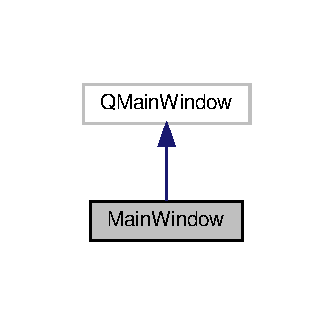
\includegraphics[width=160pt]{class_main_window__inherit__graph}
\end{center}
\end{figure}


Collaboration diagram for Main\+Window\+:
\nopagebreak
\begin{figure}[H]
\begin{center}
\leavevmode
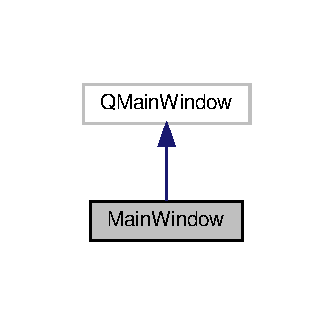
\includegraphics[width=160pt]{class_main_window__coll__graph}
\end{center}
\end{figure}
\subsection*{Public Member Functions}
\begin{DoxyCompactItemize}
\item 
\hyperlink{class_main_window_a996c5a2b6f77944776856f08ec30858d}{Main\+Window} (Q\+Widget $\ast$parent=nullptr)
\item 
\hyperlink{class_main_window_ae98d00a93bc118200eeef9f9bba1dba7}{$\sim$\+Main\+Window} ()
\end{DoxyCompactItemize}


\subsection{Detailed Description}


Definition at line 10 of file mainwindow.\+h.



\subsection{Constructor \& Destructor Documentation}
\mbox{\Hypertarget{class_main_window_a996c5a2b6f77944776856f08ec30858d}\label{class_main_window_a996c5a2b6f77944776856f08ec30858d}} 
\index{Main\+Window@{Main\+Window}!Main\+Window@{Main\+Window}}
\index{Main\+Window@{Main\+Window}!Main\+Window@{Main\+Window}}
\subsubsection{\texorpdfstring{Main\+Window()}{MainWindow()}}
{\footnotesize\ttfamily Main\+Window\+::\+Main\+Window (\begin{DoxyParamCaption}\item[{Q\+Widget $\ast$}]{parent = {\ttfamily nullptr} }\end{DoxyParamCaption})\hspace{0.3cm}{\ttfamily [explicit]}}



Definition at line 145 of file mainwindow.\+cpp.

\mbox{\Hypertarget{class_main_window_ae98d00a93bc118200eeef9f9bba1dba7}\label{class_main_window_ae98d00a93bc118200eeef9f9bba1dba7}} 
\index{Main\+Window@{Main\+Window}!````~Main\+Window@{$\sim$\+Main\+Window}}
\index{````~Main\+Window@{$\sim$\+Main\+Window}!Main\+Window@{Main\+Window}}
\subsubsection{\texorpdfstring{$\sim$\+Main\+Window()}{~MainWindow()}}
{\footnotesize\ttfamily Main\+Window\+::$\sim$\+Main\+Window (\begin{DoxyParamCaption}{ }\end{DoxyParamCaption})}



Definition at line 154 of file mainwindow.\+cpp.



The documentation for this class was generated from the following files\+:\begin{DoxyCompactItemize}
\item 
dictionary/\hyperlink{mainwindow_8h}{mainwindow.\+h}\item 
dictionary/\hyperlink{mainwindow_8cpp}{mainwindow.\+cpp}\end{DoxyCompactItemize}

\hypertarget{structqt__meta__stringdata___main_window__t}{}\section{qt\+\_\+meta\+\_\+stringdata\+\_\+\+Main\+Window\+\_\+t Struct Reference}
\label{structqt__meta__stringdata___main_window__t}\index{qt\+\_\+meta\+\_\+stringdata\+\_\+\+Main\+Window\+\_\+t@{qt\+\_\+meta\+\_\+stringdata\+\_\+\+Main\+Window\+\_\+t}}
\subsection*{Public Attributes}
\begin{DoxyCompactItemize}
\item 
Q\+Byte\+Array\+Data \hyperlink{structqt__meta__stringdata___main_window__t_a332d7fa058028f7613b5ba68abb5a7fe}{data} \mbox{[}4\mbox{]}
\item 
char \hyperlink{structqt__meta__stringdata___main_window__t_af7bc4685461b0d13618119dbb90593d5}{stringdata0} \mbox{[}43\mbox{]}
\end{DoxyCompactItemize}


\subsection{Detailed Description}


Definition at line 24 of file moc\+\_\+mainwindow.\+cpp.



\subsection{Member Data Documentation}
\mbox{\Hypertarget{structqt__meta__stringdata___main_window__t_a332d7fa058028f7613b5ba68abb5a7fe}\label{structqt__meta__stringdata___main_window__t_a332d7fa058028f7613b5ba68abb5a7fe}} 
\index{qt\+\_\+meta\+\_\+stringdata\+\_\+\+Main\+Window\+\_\+t@{qt\+\_\+meta\+\_\+stringdata\+\_\+\+Main\+Window\+\_\+t}!data@{data}}
\index{data@{data}!qt\+\_\+meta\+\_\+stringdata\+\_\+\+Main\+Window\+\_\+t@{qt\+\_\+meta\+\_\+stringdata\+\_\+\+Main\+Window\+\_\+t}}
\subsubsection{\texorpdfstring{data}{data}}
{\footnotesize\ttfamily Q\+Byte\+Array\+Data qt\+\_\+meta\+\_\+stringdata\+\_\+\+Main\+Window\+\_\+t\+::data\mbox{[}4\mbox{]}}



Definition at line 25 of file moc\+\_\+mainwindow.\+cpp.

\mbox{\Hypertarget{structqt__meta__stringdata___main_window__t_af7bc4685461b0d13618119dbb90593d5}\label{structqt__meta__stringdata___main_window__t_af7bc4685461b0d13618119dbb90593d5}} 
\index{qt\+\_\+meta\+\_\+stringdata\+\_\+\+Main\+Window\+\_\+t@{qt\+\_\+meta\+\_\+stringdata\+\_\+\+Main\+Window\+\_\+t}!stringdata0@{stringdata0}}
\index{stringdata0@{stringdata0}!qt\+\_\+meta\+\_\+stringdata\+\_\+\+Main\+Window\+\_\+t@{qt\+\_\+meta\+\_\+stringdata\+\_\+\+Main\+Window\+\_\+t}}
\subsubsection{\texorpdfstring{stringdata0}{stringdata0}}
{\footnotesize\ttfamily char qt\+\_\+meta\+\_\+stringdata\+\_\+\+Main\+Window\+\_\+t\+::stringdata0\mbox{[}43\mbox{]}}



Definition at line 26 of file moc\+\_\+mainwindow.\+cpp.



The documentation for this struct was generated from the following file\+:\begin{DoxyCompactItemize}
\item 
dictionary/\hyperlink{moc__mainwindow_8cpp}{moc\+\_\+mainwindow.\+cpp}\end{DoxyCompactItemize}

\hypertarget{struct_trie_node}{}\section{Trie\+Node Struct Reference}
\label{struct_trie_node}\index{Trie\+Node@{Trie\+Node}}


Collaboration diagram for Trie\+Node\+:
\nopagebreak
\begin{figure}[H]
\begin{center}
\leavevmode
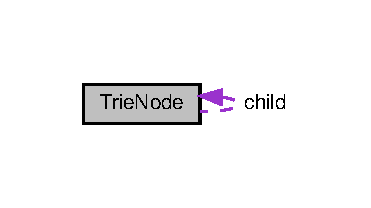
\includegraphics[width=178pt]{struct_trie_node__coll__graph}
\end{center}
\end{figure}
\subsection*{Public Attributes}
\begin{DoxyCompactItemize}
\item 
struct \hyperlink{struct_trie_node}{Trie\+Node} $\ast$ \hyperlink{struct_trie_node_a3ec9fb81441dc5f30960242580869b80}{child} \mbox{[}\hyperlink{mainwindow_8cpp_afb525552ed6d204d5636ad18ccf5355f}{A\+L\+P\+H\+A\+B\+E\+T\+\_\+\+S\+I\+ZE}\mbox{]}
\item 
bool \hyperlink{struct_trie_node_ab2732ce1e141346865d997859836d663}{is\+End\+Of\+Word}
\item 
string \hyperlink{struct_trie_node_a74b66d86de58c281d357f24e736ad953}{meaning}
\end{DoxyCompactItemize}


\subsection{Detailed Description}


Definition at line 9 of file mainwindow.\+cpp.



\subsection{Member Data Documentation}
\mbox{\Hypertarget{struct_trie_node_a3ec9fb81441dc5f30960242580869b80}\label{struct_trie_node_a3ec9fb81441dc5f30960242580869b80}} 
\index{Trie\+Node@{Trie\+Node}!child@{child}}
\index{child@{child}!Trie\+Node@{Trie\+Node}}
\subsubsection{\texorpdfstring{child}{child}}
{\footnotesize\ttfamily struct \hyperlink{struct_trie_node}{Trie\+Node}$\ast$ Trie\+Node\+::child\mbox{[}\hyperlink{mainwindow_8cpp_afb525552ed6d204d5636ad18ccf5355f}{A\+L\+P\+H\+A\+B\+E\+T\+\_\+\+S\+I\+ZE}\mbox{]}}



Definition at line 11 of file mainwindow.\+cpp.

\mbox{\Hypertarget{struct_trie_node_ab2732ce1e141346865d997859836d663}\label{struct_trie_node_ab2732ce1e141346865d997859836d663}} 
\index{Trie\+Node@{Trie\+Node}!is\+End\+Of\+Word@{is\+End\+Of\+Word}}
\index{is\+End\+Of\+Word@{is\+End\+Of\+Word}!Trie\+Node@{Trie\+Node}}
\subsubsection{\texorpdfstring{is\+End\+Of\+Word}{isEndOfWord}}
{\footnotesize\ttfamily bool Trie\+Node\+::is\+End\+Of\+Word}



Definition at line 12 of file mainwindow.\+cpp.

\mbox{\Hypertarget{struct_trie_node_a74b66d86de58c281d357f24e736ad953}\label{struct_trie_node_a74b66d86de58c281d357f24e736ad953}} 
\index{Trie\+Node@{Trie\+Node}!meaning@{meaning}}
\index{meaning@{meaning}!Trie\+Node@{Trie\+Node}}
\subsubsection{\texorpdfstring{meaning}{meaning}}
{\footnotesize\ttfamily string Trie\+Node\+::meaning}



Definition at line 13 of file mainwindow.\+cpp.



The documentation for this struct was generated from the following file\+:\begin{DoxyCompactItemize}
\item 
dictionary/\hyperlink{mainwindow_8cpp}{mainwindow.\+cpp}\end{DoxyCompactItemize}

\chapter{File Documentation}
\hypertarget{main_8cpp}{}\section{dictionary/main.cpp File Reference}
\label{main_8cpp}\index{dictionary/main.\+cpp@{dictionary/main.\+cpp}}
{\ttfamily \#include \char`\"{}mainwindow.\+h\char`\"{}}\newline
{\ttfamily \#include $<$Q\+Application$>$}\newline
Include dependency graph for main.\+cpp\+:
\nopagebreak
\begin{figure}[H]
\begin{center}
\leavevmode
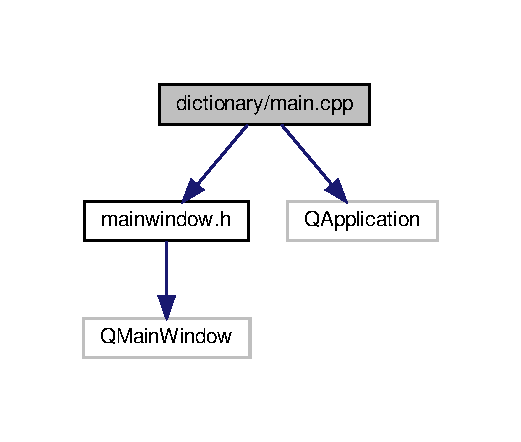
\includegraphics[width=250pt]{main_8cpp__incl}
\end{center}
\end{figure}
\subsection*{Functions}
\begin{DoxyCompactItemize}
\item 
int \hyperlink{main_8cpp_a0ddf1224851353fc92bfbff6f499fa97}{main} (int argc, char $\ast$argv\mbox{[}$\,$\mbox{]})
\end{DoxyCompactItemize}


\subsection{Function Documentation}
\mbox{\Hypertarget{main_8cpp_a0ddf1224851353fc92bfbff6f499fa97}\label{main_8cpp_a0ddf1224851353fc92bfbff6f499fa97}} 
\index{main.\+cpp@{main.\+cpp}!main@{main}}
\index{main@{main}!main.\+cpp@{main.\+cpp}}
\subsubsection{\texorpdfstring{main()}{main()}}
{\footnotesize\ttfamily int main (\begin{DoxyParamCaption}\item[{int}]{argc,  }\item[{char $\ast$}]{argv\mbox{[}$\,$\mbox{]} }\end{DoxyParamCaption})}



Definition at line 4 of file main.\+cpp.


\hypertarget{mainwindow_8cpp}{}\section{dictionary/mainwindow.cpp File Reference}
\label{mainwindow_8cpp}\index{dictionary/mainwindow.\+cpp@{dictionary/mainwindow.\+cpp}}
{\ttfamily \#include \char`\"{}mainwindow.\+h\char`\"{}}\newline
{\ttfamily \#include \char`\"{}ui\+\_\+mainwindow.\+h\char`\"{}}\newline
{\ttfamily \#include $<$Q\+File$>$}\newline
{\ttfamily \#include $<$Q\+Text\+Stream$>$}\newline
{\ttfamily \#include $<$bits/stdc++.\+h$>$}\newline
Include dependency graph for mainwindow.\+cpp\+:
\nopagebreak
\begin{figure}[H]
\begin{center}
\leavevmode
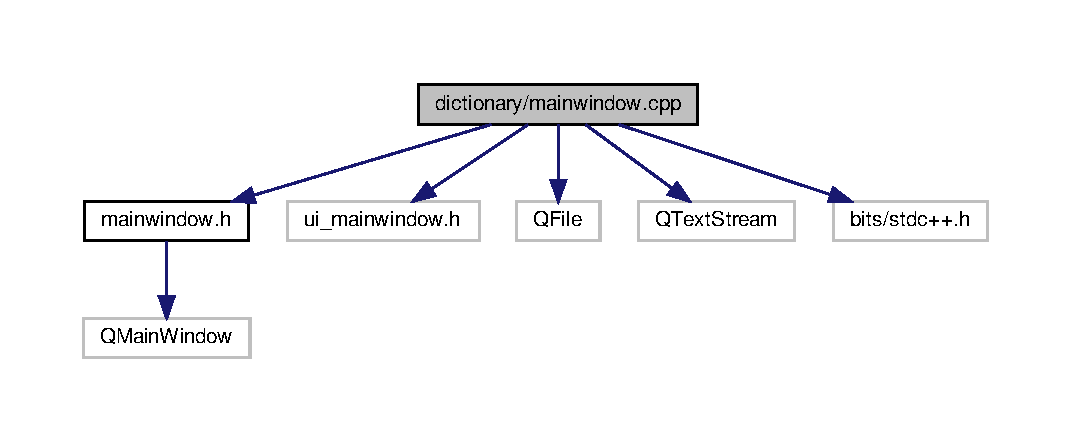
\includegraphics[width=350pt]{mainwindow_8cpp__incl}
\end{center}
\end{figure}
\subsection*{Classes}
\begin{DoxyCompactItemize}
\item 
struct \hyperlink{struct_trie_node}{Trie\+Node}
\end{DoxyCompactItemize}
\subsection*{Functions}
\begin{DoxyCompactItemize}
\item 
struct \hyperlink{struct_trie_node}{Trie\+Node} $\ast$ \hyperlink{mainwindow_8cpp_a0cbc5742145b2215c3e72a39399ba4be}{get\+Node} ()
\item 
void \hyperlink{mainwindow_8cpp_a1756f4a6c497f6bb5b8b4194c68c0c31}{insert} (struct \hyperlink{struct_trie_node}{Trie\+Node} $\ast$\hyperlink{mainwindow_8cpp_a316ef3ec13f7a45093d79eb3be22fe98}{root}, string key, string meaning)
\item 
Q\+String \hyperlink{mainwindow_8cpp_ad875b76f67d781522617c8188955aae9}{get\+Meaning} (struct \hyperlink{struct_trie_node}{Trie\+Node} $\ast$\hyperlink{mainwindow_8cpp_a316ef3ec13f7a45093d79eb3be22fe98}{root}, string key)
\item 
void \hyperlink{mainwindow_8cpp_affe0938b316f925c080ba7304009e3b5}{set\+Dictionary} (struct \hyperlink{struct_trie_node}{Trie\+Node} $\ast$\hyperlink{mainwindow_8cpp_a316ef3ec13f7a45093d79eb3be22fe98}{root}, int num\+\_\+lines)
\end{DoxyCompactItemize}
\subsection*{Variables}
\begin{DoxyCompactItemize}
\item 
const int \hyperlink{mainwindow_8cpp_afb525552ed6d204d5636ad18ccf5355f}{A\+L\+P\+H\+A\+B\+E\+T\+\_\+\+S\+I\+ZE} = 26
\item 
struct \hyperlink{struct_trie_node}{Trie\+Node} $\ast$ \hyperlink{mainwindow_8cpp_a316ef3ec13f7a45093d79eb3be22fe98}{root}
\end{DoxyCompactItemize}


\subsection{Function Documentation}
\mbox{\Hypertarget{mainwindow_8cpp_ad875b76f67d781522617c8188955aae9}\label{mainwindow_8cpp_ad875b76f67d781522617c8188955aae9}} 
\index{mainwindow.\+cpp@{mainwindow.\+cpp}!get\+Meaning@{get\+Meaning}}
\index{get\+Meaning@{get\+Meaning}!mainwindow.\+cpp@{mainwindow.\+cpp}}
\subsubsection{\texorpdfstring{get\+Meaning()}{getMeaning()}}
{\footnotesize\ttfamily Q\+String get\+Meaning (\begin{DoxyParamCaption}\item[{struct \hyperlink{struct_trie_node}{Trie\+Node} $\ast$}]{root,  }\item[{string}]{key }\end{DoxyParamCaption})}



Definition at line 49 of file mainwindow.\+cpp.

\mbox{\Hypertarget{mainwindow_8cpp_a0cbc5742145b2215c3e72a39399ba4be}\label{mainwindow_8cpp_a0cbc5742145b2215c3e72a39399ba4be}} 
\index{mainwindow.\+cpp@{mainwindow.\+cpp}!get\+Node@{get\+Node}}
\index{get\+Node@{get\+Node}!mainwindow.\+cpp@{mainwindow.\+cpp}}
\subsubsection{\texorpdfstring{get\+Node()}{getNode()}}
{\footnotesize\ttfamily struct \hyperlink{struct_trie_node}{Trie\+Node}$\ast$ get\+Node (\begin{DoxyParamCaption}{ }\end{DoxyParamCaption})}



Definition at line 16 of file mainwindow.\+cpp.

\mbox{\Hypertarget{mainwindow_8cpp_a1756f4a6c497f6bb5b8b4194c68c0c31}\label{mainwindow_8cpp_a1756f4a6c497f6bb5b8b4194c68c0c31}} 
\index{mainwindow.\+cpp@{mainwindow.\+cpp}!insert@{insert}}
\index{insert@{insert}!mainwindow.\+cpp@{mainwindow.\+cpp}}
\subsubsection{\texorpdfstring{insert()}{insert()}}
{\footnotesize\ttfamily void insert (\begin{DoxyParamCaption}\item[{struct \hyperlink{struct_trie_node}{Trie\+Node} $\ast$}]{root,  }\item[{string}]{key,  }\item[{string}]{meaning }\end{DoxyParamCaption})}



Definition at line 30 of file mainwindow.\+cpp.

\mbox{\Hypertarget{mainwindow_8cpp_affe0938b316f925c080ba7304009e3b5}\label{mainwindow_8cpp_affe0938b316f925c080ba7304009e3b5}} 
\index{mainwindow.\+cpp@{mainwindow.\+cpp}!set\+Dictionary@{set\+Dictionary}}
\index{set\+Dictionary@{set\+Dictionary}!mainwindow.\+cpp@{mainwindow.\+cpp}}
\subsubsection{\texorpdfstring{set\+Dictionary()}{setDictionary()}}
{\footnotesize\ttfamily void set\+Dictionary (\begin{DoxyParamCaption}\item[{struct \hyperlink{struct_trie_node}{Trie\+Node} $\ast$}]{root,  }\item[{int}]{num\+\_\+lines }\end{DoxyParamCaption})}



Definition at line 72 of file mainwindow.\+cpp.



\subsection{Variable Documentation}
\mbox{\Hypertarget{mainwindow_8cpp_afb525552ed6d204d5636ad18ccf5355f}\label{mainwindow_8cpp_afb525552ed6d204d5636ad18ccf5355f}} 
\index{mainwindow.\+cpp@{mainwindow.\+cpp}!A\+L\+P\+H\+A\+B\+E\+T\+\_\+\+S\+I\+ZE@{A\+L\+P\+H\+A\+B\+E\+T\+\_\+\+S\+I\+ZE}}
\index{A\+L\+P\+H\+A\+B\+E\+T\+\_\+\+S\+I\+ZE@{A\+L\+P\+H\+A\+B\+E\+T\+\_\+\+S\+I\+ZE}!mainwindow.\+cpp@{mainwindow.\+cpp}}
\subsubsection{\texorpdfstring{A\+L\+P\+H\+A\+B\+E\+T\+\_\+\+S\+I\+ZE}{ALPHABET\_SIZE}}
{\footnotesize\ttfamily const int A\+L\+P\+H\+A\+B\+E\+T\+\_\+\+S\+I\+ZE = 26}



Definition at line 8 of file mainwindow.\+cpp.

\mbox{\Hypertarget{mainwindow_8cpp_a316ef3ec13f7a45093d79eb3be22fe98}\label{mainwindow_8cpp_a316ef3ec13f7a45093d79eb3be22fe98}} 
\index{mainwindow.\+cpp@{mainwindow.\+cpp}!root@{root}}
\index{root@{root}!mainwindow.\+cpp@{mainwindow.\+cpp}}
\subsubsection{\texorpdfstring{root}{root}}
{\footnotesize\ttfamily struct \hyperlink{struct_trie_node}{Trie\+Node}$\ast$ root}



Definition at line 28 of file mainwindow.\+cpp.


\hypertarget{mainwindow_8h}{}\section{dictionary/mainwindow.h File Reference}
\label{mainwindow_8h}\index{dictionary/mainwindow.\+h@{dictionary/mainwindow.\+h}}
{\ttfamily \#include $<$Q\+Main\+Window$>$}\newline
Include dependency graph for mainwindow.\+h\+:
\nopagebreak
\begin{figure}[H]
\begin{center}
\leavevmode
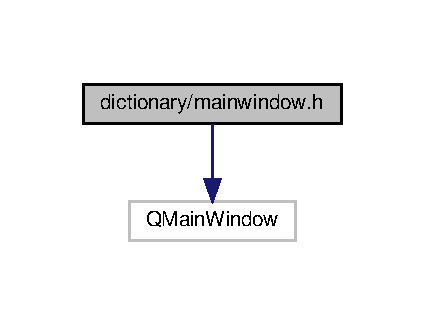
\includegraphics[width=204pt]{mainwindow_8h__incl}
\end{center}
\end{figure}
This graph shows which files directly or indirectly include this file\+:
\nopagebreak
\begin{figure}[H]
\begin{center}
\leavevmode
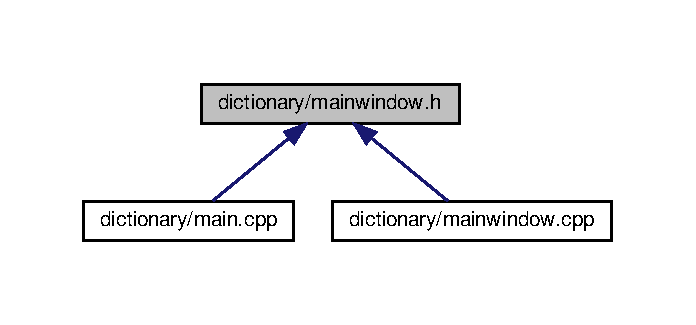
\includegraphics[width=334pt]{mainwindow_8h__dep__incl}
\end{center}
\end{figure}
\subsection*{Classes}
\begin{DoxyCompactItemize}
\item 
class \hyperlink{class_main_window}{Main\+Window}
\end{DoxyCompactItemize}
\subsection*{Namespaces}
\begin{DoxyCompactItemize}
\item 
 \hyperlink{namespace_ui}{Ui}
\end{DoxyCompactItemize}

\hypertarget{moc__mainwindow_8cpp}{}\section{dictionary/moc\+\_\+mainwindow.cpp File Reference}
\label{moc__mainwindow_8cpp}\index{dictionary/moc\+\_\+mainwindow.\+cpp@{dictionary/moc\+\_\+mainwindow.\+cpp}}
{\ttfamily \#include $<$memory$>$}\newline
{\ttfamily \#include \char`\"{}../../\+K\+A\+M\+L\+E\+S\+H/mainwindow.\+h\char`\"{}}\newline
{\ttfamily \#include $<$Qt\+Core/qbytearray.\+h$>$}\newline
{\ttfamily \#include $<$Qt\+Core/qmetatype.\+h$>$}\newline
Include dependency graph for moc\+\_\+mainwindow.\+cpp\+:
\nopagebreak
\begin{figure}[H]
\begin{center}
\leavevmode
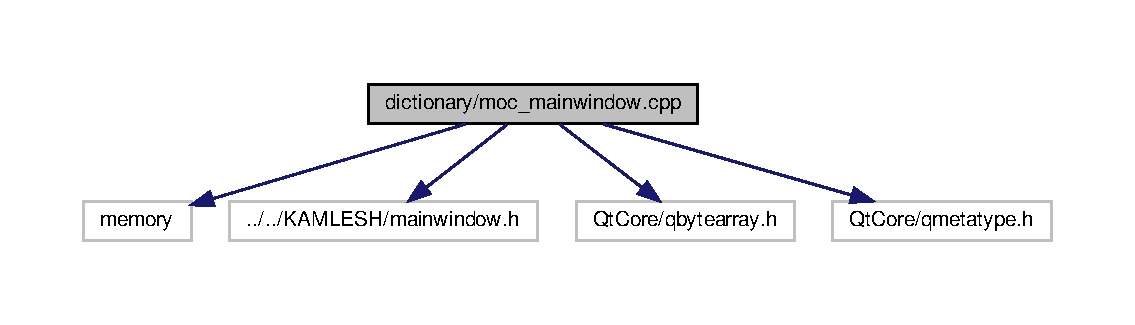
\includegraphics[width=350pt]{moc__mainwindow_8cpp__incl}
\end{center}
\end{figure}
\subsection*{Classes}
\begin{DoxyCompactItemize}
\item 
struct \hyperlink{structqt__meta__stringdata___main_window__t}{qt\+\_\+meta\+\_\+stringdata\+\_\+\+Main\+Window\+\_\+t}
\end{DoxyCompactItemize}
\subsection*{Macros}
\begin{DoxyCompactItemize}
\item 
\#define \hyperlink{moc__mainwindow_8cpp_a75bb9482d242cde0a06c9dbdc6b83abe}{Q\+T\+\_\+\+M\+O\+C\+\_\+\+L\+I\+T\+E\+R\+AL}(idx,  ofs,  len)
\end{DoxyCompactItemize}


\subsection{Macro Definition Documentation}
\mbox{\Hypertarget{moc__mainwindow_8cpp_a75bb9482d242cde0a06c9dbdc6b83abe}\label{moc__mainwindow_8cpp_a75bb9482d242cde0a06c9dbdc6b83abe}} 
\index{moc\+\_\+mainwindow.\+cpp@{moc\+\_\+mainwindow.\+cpp}!Q\+T\+\_\+\+M\+O\+C\+\_\+\+L\+I\+T\+E\+R\+AL@{Q\+T\+\_\+\+M\+O\+C\+\_\+\+L\+I\+T\+E\+R\+AL}}
\index{Q\+T\+\_\+\+M\+O\+C\+\_\+\+L\+I\+T\+E\+R\+AL@{Q\+T\+\_\+\+M\+O\+C\+\_\+\+L\+I\+T\+E\+R\+AL}!moc\+\_\+mainwindow.\+cpp@{moc\+\_\+mainwindow.\+cpp}}
\subsubsection{\texorpdfstring{Q\+T\+\_\+\+M\+O\+C\+\_\+\+L\+I\+T\+E\+R\+AL}{QT\_MOC\_LITERAL}}
{\footnotesize\ttfamily \#define Q\+T\+\_\+\+M\+O\+C\+\_\+\+L\+I\+T\+E\+R\+AL(\begin{DoxyParamCaption}\item[{}]{idx,  }\item[{}]{ofs,  }\item[{}]{len }\end{DoxyParamCaption})}

{\bfseries Value\+:}
\begin{DoxyCode}
Q\_STATIC\_BYTE\_ARRAY\_DATA\_HEADER\_INITIALIZER\_WITH\_OFFSET(len, \(\backslash\)
    qptrdiff(offsetof(\hyperlink{structqt__meta__stringdata___main_window__t}{qt\_meta\_stringdata\_MainWindow\_t}, stringdata0) + ofs \(\backslash\)
        - idx * \textcolor{keyword}{sizeof}(QByteArrayData)) \(\backslash\)
    )
\end{DoxyCode}


Definition at line 28 of file moc\+\_\+mainwindow.\+cpp.


\hypertarget{moc__predefs_8h}{}\section{dictionary/moc\+\_\+predefs.h File Reference}
\label{moc__predefs_8h}\index{dictionary/moc\+\_\+predefs.\+h@{dictionary/moc\+\_\+predefs.\+h}}
\subsection*{Macros}
\begin{DoxyCompactItemize}
\item 
\#define \hyperlink{moc__predefs_8h_a63d6f5d1c3371192fe03b3fb06e82400}{\+\_\+\+\_\+\+D\+B\+L\+\_\+\+M\+I\+N\+\_\+\+E\+X\+P\+\_\+\+\_\+}~(-\/1021)
\item 
\#define \hyperlink{moc__predefs_8h_a6605c8368985e3b1885a84d1d44ff798}{\+\_\+\+\_\+\+F\+L\+T32\+X\+\_\+\+M\+A\+X\+\_\+\+E\+X\+P\+\_\+\+\_\+}~1024
\item 
\#define \hyperlink{moc__predefs_8h_ac47e77d27e7d30f01cde452a9cd218ed}{\+\_\+\+\_\+cpp\+\_\+attributes}~200809
\item 
\#define \hyperlink{moc__predefs_8h_a6a762b969d5eea9e6a8db715a5f5a1a9}{\+\_\+\+\_\+\+U\+I\+N\+T\+\_\+\+L\+E\+A\+S\+T16\+\_\+\+M\+A\+X\+\_\+\+\_\+}~0xffff
\item 
\#define \hyperlink{moc__predefs_8h_a72e3c30a05bd2bb63d76550e451a438e}{\+\_\+\+\_\+\+A\+T\+O\+M\+I\+C\+\_\+\+A\+C\+Q\+U\+I\+RE}~2
\item 
\#define \hyperlink{moc__predefs_8h_af071b48310b9018035302c28cfd0424e}{\+\_\+\+\_\+\+F\+L\+T128\+\_\+\+M\+A\+X\+\_\+10\+\_\+\+E\+X\+P\+\_\+\+\_\+}~4932
\item 
\#define \hyperlink{moc__predefs_8h_a6e947aa0a2cb4808d560339fef0d4793}{\+\_\+\+\_\+\+F\+L\+T\+\_\+\+M\+I\+N\+\_\+\+\_\+}~1.\+17549435082228750796873653722224568e-\/38F
\item 
\#define \hyperlink{moc__predefs_8h_a779a207685ad2b8ca4cdab02ece517eb}{\+\_\+\+\_\+\+G\+C\+C\+\_\+\+I\+E\+C\+\_\+559\+\_\+\+C\+O\+M\+P\+L\+EX}~2
\item 
\#define \hyperlink{moc__predefs_8h_a5a8c0a31337df765b55c6260ef58e51e}{\+\_\+\+\_\+\+U\+I\+N\+T\+\_\+\+L\+E\+A\+S\+T8\+\_\+\+T\+Y\+P\+E\+\_\+\+\_\+}~unsigned char
\item 
\#define \hyperlink{moc__predefs_8h_acb072d4167167be73828de722a2def0b}{\+\_\+\+\_\+\+S\+I\+Z\+E\+O\+F\+\_\+\+F\+L\+O\+A\+T80\+\_\+\+\_\+}~16
\item 
\#define \hyperlink{moc__predefs_8h_a7d7e5874cd6f169187aac7db998625f3}{\+\_\+\+W\+I\+N32}~1
\item 
\#define \hyperlink{moc__predefs_8h_adb0d09cff489746c5456407aa832fced}{\+\_\+\+\_\+\+I\+N\+T\+M\+A\+X\+\_\+C}(c)~c \#\# LL
\item 
\#define \hyperlink{moc__predefs_8h_ab35e271dce6e7e2190d60b5905375419}{\+\_\+\+\_\+\+C\+H\+A\+R\+\_\+\+B\+I\+T\+\_\+\+\_\+}~8
\item 
\#define \hyperlink{moc__predefs_8h_afd12ac7489bdbbed7fa3cc51023b8f73}{\+\_\+\+\_\+\+U\+I\+N\+T8\+\_\+\+M\+A\+X\+\_\+\+\_\+}~0xff
\item 
\#define \hyperlink{moc__predefs_8h_ad1cbc0b24485be6857de50cce7e86e5d}{\+\_\+\+W\+I\+N64}~1
\item 
\#define \hyperlink{moc__predefs_8h_a8925e15bce319fa2f42c659f6a3e0199}{\+\_\+\+\_\+\+W\+I\+N\+T\+\_\+\+M\+A\+X\+\_\+\+\_\+}~0xffff
\item 
\#define \hyperlink{moc__predefs_8h_a300c6970bb64b04e45a9c2ed139ecce8}{\+\_\+\+\_\+\+F\+L\+T32\+\_\+\+M\+I\+N\+\_\+\+E\+X\+P\+\_\+\+\_\+}~(-\/125)
\item 
\#define \hyperlink{moc__predefs_8h_a60c56e472a1144b03053a2c7a2abb7fb}{\+\_\+\+\_\+cpp\+\_\+static\+\_\+assert}~200410
\item 
\#define \hyperlink{moc__predefs_8h_a2b695357ce4b46971d54e8e9dfe5724f}{\+\_\+\+\_\+\+O\+R\+D\+E\+R\+\_\+\+L\+I\+T\+T\+L\+E\+\_\+\+E\+N\+D\+I\+A\+N\+\_\+\+\_\+}~1234
\item 
\#define \hyperlink{moc__predefs_8h_a66fbb70a69c9f66830f95a20e46091a6}{\+\_\+\+\_\+\+S\+I\+Z\+E\+\_\+\+M\+A\+X\+\_\+\+\_\+}~0xffffffffffffffff\+U\+LL
\item 
\#define \hyperlink{moc__predefs_8h_a65ac8cd0434319a3a31dc031409c218a}{\+\_\+\+\_\+\+W\+C\+H\+A\+R\+\_\+\+M\+A\+X\+\_\+\+\_\+}~0xffff
\item 
\#define \hyperlink{moc__predefs_8h_a33433eca9e18e14156165252746f4d44}{\+\_\+\+\_\+\+G\+C\+C\+\_\+\+H\+A\+V\+E\+\_\+\+S\+Y\+N\+C\+\_\+\+C\+O\+M\+P\+A\+R\+E\+\_\+\+A\+N\+D\+\_\+\+S\+W\+A\+P\+\_\+1}~1
\item 
\#define \hyperlink{moc__predefs_8h_a7237ce09defceeebe3ba0afc528275ac}{\+\_\+\+\_\+\+G\+C\+C\+\_\+\+H\+A\+V\+E\+\_\+\+S\+Y\+N\+C\+\_\+\+C\+O\+M\+P\+A\+R\+E\+\_\+\+A\+N\+D\+\_\+\+S\+W\+A\+P\+\_\+2}~1
\item 
\#define \hyperlink{moc__predefs_8h_a6310789290c9c5717826b56443ce69ec}{\+\_\+\+\_\+\+G\+C\+C\+\_\+\+H\+A\+V\+E\+\_\+\+S\+Y\+N\+C\+\_\+\+C\+O\+M\+P\+A\+R\+E\+\_\+\+A\+N\+D\+\_\+\+S\+W\+A\+P\+\_\+4}~1
\item 
\#define \hyperlink{moc__predefs_8h_aca2a716d3e84ccffe000390bb2e2fb38}{\+\_\+\+\_\+\+D\+B\+L\+\_\+\+D\+E\+N\+O\+R\+M\+\_\+\+M\+I\+N\+\_\+\+\_\+}~double(4.\+94065645841246544176568792868221372e-\/324\+L)
\item 
\#define \hyperlink{moc__predefs_8h_a86bb5059d696b19082c1aff4ae93a87a}{\+\_\+\+\_\+\+G\+C\+C\+\_\+\+H\+A\+V\+E\+\_\+\+S\+Y\+N\+C\+\_\+\+C\+O\+M\+P\+A\+R\+E\+\_\+\+A\+N\+D\+\_\+\+S\+W\+A\+P\+\_\+8}~1
\item 
\#define \hyperlink{moc__predefs_8h_a403ff8d656461ff5a083fb47f73c7da3}{\+\_\+\+\_\+\+G\+C\+C\+\_\+\+A\+T\+O\+M\+I\+C\+\_\+\+C\+H\+A\+R\+\_\+\+L\+O\+C\+K\+\_\+\+F\+R\+EE}~2
\item 
\#define \hyperlink{moc__predefs_8h_a0a3bd26d0b040f0781a238e4aedd3dbe}{\+\_\+\+\_\+\+G\+C\+C\+\_\+\+I\+E\+C\+\_\+559}~2
\item 
\#define \hyperlink{moc__predefs_8h_a00a9f6ceb42fbe18b789b4c1949c49f2}{\+\_\+\+\_\+\+F\+L\+T32\+X\+\_\+\+D\+E\+C\+I\+M\+A\+L\+\_\+\+D\+I\+G\+\_\+\+\_\+}~17
\item 
\#define \hyperlink{moc__predefs_8h_a737828904768e0ab49acbdb3371d8445}{\+\_\+\+\_\+\+F\+L\+T\+\_\+\+E\+V\+A\+L\+\_\+\+M\+E\+T\+H\+O\+D\+\_\+\+\_\+}~0
\item 
\#define \hyperlink{moc__predefs_8h_ade9dc15e022182eb0a62a0fd17d18b75}{\+\_\+\+\_\+cpp\+\_\+binary\+\_\+literals}~201304
\item 
\#define \hyperlink{moc__predefs_8h_a8ef55ba782e9d01cb22911f97168d06a}{\+\_\+\+\_\+\+F\+L\+T64\+\_\+\+D\+E\+C\+I\+M\+A\+L\+\_\+\+D\+I\+G\+\_\+\+\_\+}~17
\item 
\#define \hyperlink{moc__predefs_8h_a98e298953067135caf4bc0b8e8e7cd01}{\+\_\+\+\_\+\+G\+C\+C\+\_\+\+A\+T\+O\+M\+I\+C\+\_\+\+C\+H\+A\+R32\+\_\+\+T\+\_\+\+L\+O\+C\+K\+\_\+\+F\+R\+EE}~2
\item 
\#define \hyperlink{moc__predefs_8h_a64b6ba77bbc2cb5db2a19f32e954fcc3}{\+\_\+\+\_\+x86\+\_\+64}~1
\item 
\#define \hyperlink{moc__predefs_8h_a559dd2b0792fc2b0b30ba1dd66ca7cdc}{\+\_\+\+\_\+cpp\+\_\+variadic\+\_\+templates}~200704
\item 
\#define \hyperlink{moc__predefs_8h_a17a1ff08595cf7e0c9d1f162b727ccb6}{\+\_\+\+\_\+\+U\+I\+N\+T\+\_\+\+F\+A\+S\+T64\+\_\+\+M\+A\+X\+\_\+\+\_\+}~0xffffffffffffffff\+U\+LL
\item 
\#define \hyperlink{moc__predefs_8h_ac60fe3845f87fdaf6365a733ede87cfe}{\+\_\+\+\_\+\+S\+I\+G\+\_\+\+A\+T\+O\+M\+I\+C\+\_\+\+T\+Y\+P\+E\+\_\+\+\_\+}~int
\item 
\#define \hyperlink{moc__predefs_8h_a1abd7cf346a460459d7fe1a9d4b5dde9}{\+\_\+\+\_\+\+D\+B\+L\+\_\+\+M\+I\+N\+\_\+10\+\_\+\+E\+X\+P\+\_\+\+\_\+}~(-\/307)
\item 
\#define \hyperlink{moc__predefs_8h_a611d40c375b1972669292fd27bc4afb7}{\+\_\+\+\_\+\+F\+I\+N\+I\+T\+E\+\_\+\+M\+A\+T\+H\+\_\+\+O\+N\+L\+Y\+\_\+\+\_\+}~0
\item 
\#define \hyperlink{moc__predefs_8h_ad149c0565fcf669b23f483e5b7f80dbd}{\+\_\+\+\_\+\+G\+N\+U\+C\+\_\+\+P\+A\+T\+C\+H\+L\+E\+V\+E\+L\+\_\+\+\_\+}~0
\item 
\#define \hyperlink{moc__predefs_8h_ac1175c9478c586edee06d1f788a03b83}{\+\_\+\+\_\+\+F\+L\+T32\+\_\+\+H\+A\+S\+\_\+\+D\+E\+N\+O\+R\+M\+\_\+\+\_\+}~1
\item 
\#define \hyperlink{moc__predefs_8h_a27b5eb7cfda61c7f1baeb4d95f3052bb}{\+\_\+\+\_\+\+U\+I\+N\+T\+\_\+\+F\+A\+S\+T8\+\_\+\+M\+A\+X\+\_\+\+\_\+}~0xff
\item 
\#define \hyperlink{moc__predefs_8h_a1c6886956b05c16006d924f77a868410}{\+\_\+\+\_\+has\+\_\+include}(S\+TR)~\+\_\+\+\_\+has\+\_\+include\+\_\+\+\_\+(S\+TR)
\item 
\#define \hyperlink{moc__predefs_8h_a3107b1d0ca10d4ae4575d9107d4cbffe}{\+\_\+stdcall}~\+\_\+\+\_\+attribute\+\_\+\+\_\+((\+\_\+\+\_\+stdcall\+\_\+\+\_\+))
\item 
\#define \hyperlink{moc__predefs_8h_a3d4fe0f0b2e3ae12569d4a663dee8a0c}{\+\_\+\+\_\+\+D\+E\+C64\+\_\+\+M\+A\+X\+\_\+\+E\+X\+P\+\_\+\+\_\+}~385
\item 
\#define \hyperlink{moc__predefs_8h_ad36bc14a0433c9f88496bed4ccbd65a3}{\+\_\+\+\_\+\+I\+N\+T8\+\_\+C}(c)~c
\item 
\#define \hyperlink{moc__predefs_8h_a967b4ada96d28b97bc07e26e1def8e66}{\+\_\+\+\_\+\+I\+N\+T\+\_\+\+L\+E\+A\+S\+T8\+\_\+\+W\+I\+D\+T\+H\+\_\+\+\_\+}~8
\item 
\#define \hyperlink{moc__predefs_8h_a4bf843ffcadf9b162b74c1b7e546e8e9}{\+\_\+\+\_\+\+U\+I\+N\+T\+\_\+\+L\+E\+A\+S\+T64\+\_\+\+M\+A\+X\+\_\+\+\_\+}~0xffffffffffffffff\+U\+LL
\item 
\#define \hyperlink{moc__predefs_8h_a4f69990d03f9fb0c390a6fbad28a737b}{\+\_\+\+\_\+\+S\+H\+R\+T\+\_\+\+M\+A\+X\+\_\+\+\_\+}~0x7fff
\item 
\#define \hyperlink{moc__predefs_8h_a06fd91f0507a4f364e469c8055f4265a}{\+\_\+\+\_\+\+L\+D\+B\+L\+\_\+\+M\+A\+X\+\_\+\+\_\+}~1.\+18973149535723176502126385303097021e+4932L
\item 
\#define \hyperlink{moc__predefs_8h_af707469f32a983b229e6c7e0e4efc063}{\+\_\+\+\_\+\+F\+L\+T64\+X\+\_\+\+M\+A\+X\+\_\+10\+\_\+\+E\+X\+P\+\_\+\+\_\+}~4932
\item 
\#define \hyperlink{moc__predefs_8h_aaf06a1464d33431377a2ee5293ec70d2}{\+\_\+\+\_\+\+U\+I\+N\+T\+\_\+\+L\+E\+A\+S\+T8\+\_\+\+M\+A\+X\+\_\+\+\_\+}~0xff
\item 
\#define \hyperlink{moc__predefs_8h_a9685ff8e617f3c5892c2a6fe3484f3b7}{\+\_\+\+\_\+\+G\+C\+C\+\_\+\+A\+T\+O\+M\+I\+C\+\_\+\+B\+O\+O\+L\+\_\+\+L\+O\+C\+K\+\_\+\+F\+R\+EE}~2
\item 
\#define \hyperlink{moc__predefs_8h_a960cb27a87591af89eddb328647f1534}{\+\_\+\+\_\+\+F\+L\+T128\+\_\+\+D\+E\+N\+O\+R\+M\+\_\+\+M\+I\+N\+\_\+\+\_\+}~6.\+47517511943802511092443895822764655e-\/4966\+F128
\item 
\#define \hyperlink{moc__predefs_8h_ab86380373ae9fa385c8a2464023774a8}{\+\_\+\+\_\+\+U\+I\+N\+T\+M\+A\+X\+\_\+\+T\+Y\+P\+E\+\_\+\+\_\+}~long long unsigned int
\item 
\#define \hyperlink{moc__predefs_8h_a13526b223391d4982c4c172c29bfdc1e}{\+\_\+\+\_\+\+D\+E\+C32\+\_\+\+E\+P\+S\+I\+L\+O\+N\+\_\+\+\_\+}~1\+E-\/6\+DF
\item 
\#define \hyperlink{moc__predefs_8h_af635b5d104ef9858a68ab2c56677fd2d}{\+\_\+\+\_\+\+F\+L\+T\+\_\+\+E\+V\+A\+L\+\_\+\+M\+E\+T\+H\+O\+D\+\_\+\+T\+S\+\_\+18661\+\_\+3\+\_\+\+\_\+}~0
\item 
\#define \hyperlink{moc__predefs_8h_a5bcf2962d7a37c34484cef13fa9601b2}{\+\_\+\+\_\+\+O\+P\+T\+I\+M\+I\+Z\+E\+\_\+\+\_\+}~1
\item 
\#define \hyperlink{moc__predefs_8h_ab4425dccbcddb2363a2a8a67367a5b42}{\+\_\+\+\_\+\+U\+I\+N\+T32\+\_\+\+M\+A\+X\+\_\+\+\_\+}~0xffffffffU
\item 
\#define \hyperlink{moc__predefs_8h_a213133a8dca206becf88c2e3523b124a}{\+\_\+\+\_\+\+G\+X\+X\+\_\+\+E\+X\+P\+E\+R\+I\+M\+E\+N\+T\+A\+L\+\_\+\+C\+X\+X0\+X\+\_\+\+\_\+}~1
\item 
\#define \hyperlink{moc__predefs_8h_ae221a8e373285cf10c22926762f477f5}{\+\_\+\+\_\+\+L\+D\+B\+L\+\_\+\+M\+A\+X\+\_\+\+E\+X\+P\+\_\+\+\_\+}~16384
\item 
\#define \hyperlink{moc__predefs_8h_aad2e8f7e8d06ab966a1210f4a7d65770}{\+\_\+\+\_\+\+F\+L\+T128\+\_\+\+M\+I\+N\+\_\+\+E\+X\+P\+\_\+\+\_\+}~(-\/16381)
\item 
\#define \hyperlink{moc__predefs_8h_a135696718aa5b38e58be73aaece6654f}{\+\_\+\+\_\+\+W\+I\+N\+T\+\_\+\+M\+I\+N\+\_\+\+\_\+}~0
\item 
\#define \hyperlink{moc__predefs_8h_a784d5a4b7494076d83772a819916b039}{\+\_\+\+\_\+\+F\+L\+T128\+\_\+\+M\+I\+N\+\_\+10\+\_\+\+E\+X\+P\+\_\+\+\_\+}~(-\/4931)
\item 
\#define \hyperlink{moc__predefs_8h_a6091ba87f9a538a9685b7997a64a64db}{\+\_\+\+\_\+\+I\+N\+T\+\_\+\+L\+E\+A\+S\+T16\+\_\+\+W\+I\+D\+T\+H\+\_\+\+\_\+}~16
\item 
\#define \hyperlink{moc__predefs_8h_a87b7ceac2198cab045e40c9a64b11679}{\+\_\+\+\_\+\+S\+C\+H\+A\+R\+\_\+\+M\+A\+X\+\_\+\+\_\+}~0x7f
\item 
\#define \hyperlink{moc__predefs_8h_a39e5016b6c2adbc3a6b1674c458d4dc5}{\+\_\+\+\_\+\+F\+L\+T128\+\_\+\+M\+A\+N\+T\+\_\+\+D\+I\+G\+\_\+\+\_\+}~113
\item 
\#define \hyperlink{moc__predefs_8h_a01b915d3ec5439de746f1d5e9f76dc3d}{\+\_\+\+\_\+\+W\+C\+H\+A\+R\+\_\+\+M\+I\+N\+\_\+\+\_\+}~0
\item 
\#define \hyperlink{moc__predefs_8h_a4b8971e411b88166747d2a3c2425eaee}{\+\_\+\+\_\+\+I\+N\+T64\+\_\+C}(c)~c \#\# LL
\item 
\#define \hyperlink{moc__predefs_8h_a61969667ef3b668024a20df9bc34c991}{\+\_\+\+\_\+\+D\+B\+L\+\_\+\+D\+I\+G\+\_\+\+\_\+}~15
\item 
\#define \hyperlink{moc__predefs_8h_aa808bc3159395526ac0c07d36b87dec1}{\+\_\+\+\_\+\+G\+C\+C\+\_\+\+A\+T\+O\+M\+I\+C\+\_\+\+P\+O\+I\+N\+T\+E\+R\+\_\+\+L\+O\+C\+K\+\_\+\+F\+R\+EE}~2
\item 
\#define \hyperlink{moc__predefs_8h_ac070fafc444399b9243e0366b4ce4ef7}{\+\_\+\+\_\+\+F\+L\+T64\+X\+\_\+\+M\+A\+N\+T\+\_\+\+D\+I\+G\+\_\+\+\_\+}~64
\item 
\#define \hyperlink{moc__predefs_8h_a4b2be09502f3fe1cd13838c6761803b3}{\+\_\+\+\_\+\+S\+I\+Z\+E\+O\+F\+\_\+\+I\+N\+T\+\_\+\+\_\+}~4
\item 
\#define \hyperlink{moc__predefs_8h_a8bd657ce95940b7c6087cf5aa54d5280}{\+\_\+\+\_\+\+S\+I\+Z\+E\+O\+F\+\_\+\+P\+O\+I\+N\+T\+E\+R\+\_\+\+\_\+}~8
\item 
\#define \hyperlink{moc__predefs_8h_a7f18358ae5a65523140cb561bbeaa3a9}{\+\_\+\+\_\+\+G\+C\+C\+\_\+\+A\+T\+O\+M\+I\+C\+\_\+\+C\+H\+A\+R16\+\_\+\+T\+\_\+\+L\+O\+C\+K\+\_\+\+F\+R\+EE}~2
\item 
\#define \hyperlink{moc__predefs_8h_aff6bf0ff0fa3b5cbd23a8ae1131c87a9}{\+\_\+\+\_\+\+U\+S\+E\+R\+\_\+\+L\+A\+B\+E\+L\+\_\+\+P\+R\+E\+F\+I\+X\+\_\+\+\_\+}
\item 
\#define \hyperlink{moc__predefs_8h_a098c7fe44eed71241990da5db8f99bc3}{\+\_\+\+\_\+\+F\+L\+T64\+X\+\_\+\+E\+P\+S\+I\+L\+O\+N\+\_\+\+\_\+}~1.\+08420217248550443400745280086994171e-\/19\+F64x
\item 
\#define \hyperlink{moc__predefs_8h_a309fa84aefd09132258bbe21c20ef7d4}{\+\_\+\+\_\+\+S\+T\+D\+C\+\_\+\+H\+O\+S\+T\+E\+D\+\_\+\+\_\+}~1
\item 
\#define \hyperlink{moc__predefs_8h_a226cabdf73812d8319920ffb07154f87}{\+\_\+\+\_\+\+W\+I\+N32}~1
\item 
\#define \hyperlink{moc__predefs_8h_a87140cc80075e8907e7bbfd910c5642a}{\+\_\+\+\_\+\+L\+D\+B\+L\+\_\+\+H\+A\+S\+\_\+\+I\+N\+F\+I\+N\+I\+T\+Y\+\_\+\+\_\+}~1
\item 
\#define \hyperlink{moc__predefs_8h_a7b37ac70dc218969bf0176916a957f6f}{\+\_\+\+\_\+\+W\+I\+N64}~1
\item 
\#define \hyperlink{moc__predefs_8h_aa021702c3b7627dccaa51c33a2c5a8d1}{\+\_\+\+\_\+\+F\+L\+T32\+\_\+\+D\+I\+G\+\_\+\+\_\+}~6
\item 
\#define \hyperlink{moc__predefs_8h_a7ac5a3b1dc00b508a391f8c6c37e2165}{\+\_\+\+\_\+\+F\+L\+T\+\_\+\+E\+P\+S\+I\+L\+O\+N\+\_\+\+\_\+}~1.\+19209289550781250000000000000000000e-\/7F
\item 
\#define \hyperlink{moc__predefs_8h_afb5a2a4891df4551832357e97c6c3c59}{\+\_\+\+\_\+\+G\+X\+X\+\_\+\+W\+E\+A\+K\+\_\+\+\_\+}~1
\item 
\#define \hyperlink{moc__predefs_8h_aeb2d8312284d49b1e44c7d003bd8b54b}{\+\_\+\+\_\+\+S\+H\+R\+T\+\_\+\+W\+I\+D\+T\+H\+\_\+\+\_\+}~16
\item 
\#define \hyperlink{moc__predefs_8h_ab572f59c4b0c5a1f4c2953f38a76d7b3}{\+\_\+\+\_\+\+L\+D\+B\+L\+\_\+\+M\+I\+N\+\_\+\+\_\+}~3.\+36210314311209350626267781732175260e-\/4932L
\item 
\#define \hyperlink{moc__predefs_8h_ad3165a97a460b88ccdea80967918f250}{\+\_\+\+\_\+\+D\+E\+C32\+\_\+\+M\+A\+X\+\_\+\+\_\+}~9.\+999999\+E96\+DF
\item 
\#define \hyperlink{moc__predefs_8h_aaa322b38474911c60e45134194bd6e8f}{\+\_\+\+\_\+cpp\+\_\+threadsafe\+\_\+static\+\_\+init}~200806
\item 
\#define \hyperlink{moc__predefs_8h_ac0fe3e739d0b847c07dde20eabf2ab3d}{\+\_\+\+\_\+\+F\+L\+T64\+X\+\_\+\+D\+E\+N\+O\+R\+M\+\_\+\+M\+I\+N\+\_\+\+\_\+}~3.\+64519953188247460252840593361941982e-\/4951\+F64x
\item 
\#define \hyperlink{moc__predefs_8h_a58bb9ff70f3a05d2794468e3d6bcba26}{\+\_\+\+\_\+\+M\+I\+N\+G\+W32\+\_\+\+\_\+}~1
\item 
\#define \hyperlink{moc__predefs_8h_a8f246ad899706f78b8dfcd33daff7b07}{\+\_\+\+\_\+\+F\+L\+T32\+X\+\_\+\+H\+A\+S\+\_\+\+I\+N\+F\+I\+N\+I\+T\+Y\+\_\+\+\_\+}~1
\item 
\#define \hyperlink{moc__predefs_8h_abf681096fa9e21512a3fe83f0dcfdb36}{\+\_\+\+\_\+\+I\+N\+T32\+\_\+\+M\+A\+X\+\_\+\+\_\+}~0x7fffffff
\item 
\#define \hyperlink{moc__predefs_8h_ad3907b8d9bb2265255e6e0d66d91d165}{\+\_\+\+\_\+\+I\+N\+T\+\_\+\+W\+I\+D\+T\+H\+\_\+\+\_\+}~32
\item 
\#define \hyperlink{moc__predefs_8h_aaa8084a56e3732008acafea8fd15eb2f}{\+\_\+\+\_\+\+S\+I\+Z\+E\+O\+F\+\_\+\+L\+O\+N\+G\+\_\+\+\_\+}~4
\item 
\#define \hyperlink{moc__predefs_8h_aa860a111dcff819d3502dda14f8ac778}{\+\_\+\+\_\+\+U\+I\+N\+T16\+\_\+C}(c)~c
\item 
\#define \hyperlink{moc__predefs_8h_a96b511bfa61e4203ec3668fb39063309}{\+\_\+\+\_\+\+P\+T\+R\+D\+I\+F\+F\+\_\+\+W\+I\+D\+T\+H\+\_\+\+\_\+}~64
\item 
\#define \hyperlink{moc__predefs_8h_aeb56455e98000942147dfd63ec1c2fa6}{\+\_\+\+\_\+\+D\+E\+C\+I\+M\+A\+L\+\_\+\+D\+I\+G\+\_\+\+\_\+}~21
\item 
\#define \hyperlink{moc__predefs_8h_ad293ff29c0ac9a6b4187d366d6de3772}{\+\_\+\+\_\+\+F\+L\+T64\+\_\+\+E\+P\+S\+I\+L\+O\+N\+\_\+\+\_\+}~2.\+22044604925031308084726333618164062e-\/16\+F64
\item 
\#define \hyperlink{moc__predefs_8h_a4e8a5398566f8b2666a8a71b2dbcf3ca}{\+\_\+\+\_\+\+I\+N\+T\+M\+A\+X\+\_\+\+W\+I\+D\+T\+H\+\_\+\+\_\+}~64
\item 
\#define \hyperlink{moc__predefs_8h_aceda5e62622b9783846d26610d038f71}{\+\_\+\+\_\+\+F\+L\+T64\+\_\+\+M\+I\+N\+\_\+\+E\+X\+P\+\_\+\+\_\+}~(-\/1021)
\item 
\#define \hyperlink{moc__predefs_8h_a370369ba2463363de726ff9394861a2b}{\+\_\+\+\_\+has\+\_\+include\+\_\+next}(S\+TR)~\+\_\+\+\_\+has\+\_\+include\+\_\+next\+\_\+\+\_\+(S\+TR)
\item 
\#define \hyperlink{moc__predefs_8h_ad2396317be1036fdc4481d54343487de}{\+\_\+\+\_\+\+F\+L\+T64\+X\+\_\+\+M\+I\+N\+\_\+10\+\_\+\+E\+X\+P\+\_\+\+\_\+}~(-\/4931)
\item 
\#define \hyperlink{moc__predefs_8h_a10a15ae17c3b791fe9b9721965ebfee4}{\+\_\+\+\_\+\+L\+D\+B\+L\+\_\+\+H\+A\+S\+\_\+\+Q\+U\+I\+E\+T\+\_\+\+N\+A\+N\+\_\+\+\_\+}~1
\item 
\#define \hyperlink{moc__predefs_8h_a6c163c6e58545740cbae55ad8ffa027f}{\+\_\+\+\_\+\+F\+L\+T64\+\_\+\+M\+A\+N\+T\+\_\+\+D\+I\+G\+\_\+\+\_\+}~53
\item 
\#define \hyperlink{moc__predefs_8h_ac15da069257627fefd71d875d538b73d}{\+\_\+\+R\+E\+E\+N\+T\+R\+A\+NT}~1
\item 
\#define \hyperlink{moc__predefs_8h_aa51016843ec55a0a9df7ce9f85767ee7}{\+\_\+\+\_\+\+G\+N\+U\+C\+\_\+\+\_\+}~7
\item 
\#define \hyperlink{moc__predefs_8h_a69a11fc07c17e6dd1fa428622bff8d89}{\+\_\+cdecl}~\+\_\+\+\_\+attribute\+\_\+\+\_\+((\+\_\+\+\_\+cdecl\+\_\+\+\_\+))
\item 
\#define \hyperlink{moc__predefs_8h_af607715c8c9a98aa72c81c6629554b0d}{\+\_\+\+\_\+\+G\+X\+X\+\_\+\+R\+T\+TI}~1
\item 
\#define \hyperlink{moc__predefs_8h_ab61dd6e368adb90e2eff5739188b0bcb}{\+\_\+\+\_\+\+M\+M\+X\+\_\+\+\_\+}~1
\item 
\#define \hyperlink{moc__predefs_8h_a9e077def8c310cdb5fef37666a92c5a5}{\+\_\+\+\_\+cpp\+\_\+delegating\+\_\+constructors}~200604
\item 
\#define \hyperlink{moc__predefs_8h_a82a2c3ff271d1685b450975ffa68544a}{\+\_\+\+\_\+\+F\+L\+T\+\_\+\+H\+A\+S\+\_\+\+D\+E\+N\+O\+R\+M\+\_\+\+\_\+}~1
\item 
\#define \hyperlink{moc__predefs_8h_aae92712264b830cd7d24d4b81d502ffb}{\+\_\+\+\_\+\+S\+I\+Z\+E\+O\+F\+\_\+\+L\+O\+N\+G\+\_\+\+D\+O\+U\+B\+L\+E\+\_\+\+\_\+}~16
\item 
\#define \hyperlink{moc__predefs_8h_a2c25ec0f0ae74f9d8a7c373288a28dd1}{\+\_\+\+\_\+\+B\+I\+G\+G\+E\+S\+T\+\_\+\+A\+L\+I\+G\+N\+M\+E\+N\+T\+\_\+\+\_\+}~16
\item 
\#define \hyperlink{moc__predefs_8h_a93a5a9d251e5bff3c2a130627f20e782}{\+\_\+\+\_\+\+S\+T\+D\+C\+\_\+\+U\+T\+F\+\_\+16\+\_\+\+\_\+}~1
\item 
\#define \hyperlink{moc__predefs_8h_aeb14f5cf7cca3a01c2f6a0015e981eb1}{\+\_\+\+\_\+\+F\+L\+T64\+\_\+\+M\+A\+X\+\_\+10\+\_\+\+E\+X\+P\+\_\+\+\_\+}~308
\item 
\#define \hyperlink{moc__predefs_8h_a170219070ed7bdfea9f88121c9abbaea}{\+\_\+\+\_\+\+F\+L\+T32\+\_\+\+H\+A\+S\+\_\+\+I\+N\+F\+I\+N\+I\+T\+Y\+\_\+\+\_\+}~1
\item 
\#define \hyperlink{moc__predefs_8h_a711d7b7f27671b10b11a74c37f653ad7}{\+\_\+\+\_\+\+D\+B\+L\+\_\+\+M\+A\+X\+\_\+\+\_\+}~double(1.\+79769313486231570814527423731704357e+308\+L)
\item 
\#define \hyperlink{moc__predefs_8h_af0008e4120ef45071f4052b2f7da1e2a}{\+\_\+thiscall}~\+\_\+\+\_\+attribute\+\_\+\+\_\+((\+\_\+\+\_\+thiscall\+\_\+\+\_\+))
\item 
\#define \hyperlink{moc__predefs_8h_a7377e1bc6bd2fd9bcfe98283ab0e9037}{\+\_\+\+\_\+cpp\+\_\+raw\+\_\+strings}~200710
\item 
\#define \hyperlink{moc__predefs_8h_a84479d2bbe1d7286f406fcc302f41376}{\+\_\+\+\_\+\+I\+N\+T\+\_\+\+F\+A\+S\+T32\+\_\+\+M\+A\+X\+\_\+\+\_\+}~0x7fffffff
\item 
\#define \hyperlink{moc__predefs_8h_a45cd9660bf8cfec983f7164063381a41}{\+\_\+\+\_\+\+W\+I\+N\+NT}~1
\item 
\#define \hyperlink{moc__predefs_8h_a3dd03066dbb351dfa51353c80a7902a2}{\+\_\+\+\_\+\+D\+B\+L\+\_\+\+H\+A\+S\+\_\+\+I\+N\+F\+I\+N\+I\+T\+Y\+\_\+\+\_\+}~1
\item 
\#define \hyperlink{moc__predefs_8h_aa3f186f612efe5edfcc371c95617f06f}{\+\_\+\+\_\+\+I\+N\+T64\+\_\+\+M\+A\+X\+\_\+\+\_\+}~0x7fffffffffffffff\+LL
\item 
\#define \hyperlink{moc__predefs_8h_a942513c472dbe88bf910b8abaad21f64}{\+\_\+\+\_\+\+W\+I\+N\+N\+T\+\_\+\+\_\+}~1
\item 
\#define \hyperlink{moc__predefs_8h_a79e289c54a8c9851b2b118d442bbc26c}{\+\_\+\+\_\+\+D\+E\+C32\+\_\+\+M\+I\+N\+\_\+\+E\+X\+P\+\_\+\+\_\+}~(-\/94)
\item 
\#define \hyperlink{moc__predefs_8h_a8394afe92148ddbdf0e0697978cd1382}{\+\_\+\+\_\+\+I\+N\+T\+P\+T\+R\+\_\+\+W\+I\+D\+T\+H\+\_\+\+\_\+}~64
\item 
\#define \hyperlink{moc__predefs_8h_a97163404b3b71f857e35be74607f88f7}{\+\_\+\+\_\+\+F\+L\+T32\+X\+\_\+\+H\+A\+S\+\_\+\+D\+E\+N\+O\+R\+M\+\_\+\+\_\+}~1
\item 
\#define \hyperlink{moc__predefs_8h_a6a4d11835d03027f3929b84fe7b55bf6}{\+\_\+\+\_\+\+I\+N\+T\+\_\+\+F\+A\+S\+T16\+\_\+\+T\+Y\+P\+E\+\_\+\+\_\+}~short int
\item 
\#define \hyperlink{moc__predefs_8h_a2a2ef56cf6c226f982bdb07bcd9197c9}{\+\_\+fastcall}~\+\_\+\+\_\+attribute\+\_\+\+\_\+((\+\_\+\+\_\+fastcall\+\_\+\+\_\+))
\item 
\#define \hyperlink{moc__predefs_8h_a3c7f3130e367d47bcc27a0a41278155e}{\+\_\+\+\_\+\+L\+D\+B\+L\+\_\+\+H\+A\+S\+\_\+\+D\+E\+N\+O\+R\+M\+\_\+\+\_\+}~1
\item 
\#define \hyperlink{moc__predefs_8h_a1b391bc7ed92f79666c4a5d840aa1edd}{\+\_\+\+\_\+cplusplus}~201103L
\item 
\#define \hyperlink{moc__predefs_8h_af73192acc2dd2095bd3524ca5ee9dca9}{\+\_\+\+\_\+cpp\+\_\+ref\+\_\+qualifiers}~200710
\item 
\#define \hyperlink{moc__predefs_8h_aaab7817ee2e4bb88b5178e101e7ab2a6}{\+\_\+\+\_\+\+D\+E\+C128\+\_\+\+M\+A\+X\+\_\+\+\_\+}~9.\+999999999999999999999999999999999\+E6144\+DL
\item 
\#define \hyperlink{moc__predefs_8h_a97e13c059a63d2d547cc4a9f386641d2}{\+\_\+\+\_\+\+I\+N\+T\+\_\+\+L\+E\+A\+S\+T32\+\_\+\+M\+A\+X\+\_\+\+\_\+}~0x7fffffff
\item 
\#define \hyperlink{moc__predefs_8h_a1f993b902b5b1dba7d5b043d0abc347b}{\+\_\+\+\_\+\+D\+E\+C32\+\_\+\+M\+I\+N\+\_\+\+\_\+}~1\+E-\/95\+DF
\item 
\#define \hyperlink{moc__predefs_8h_aa806e8f7ce2a8db3bf676735fca2ac51}{\+\_\+\+\_\+\+D\+E\+P\+R\+E\+C\+A\+T\+ED}~1
\item 
\#define \hyperlink{moc__predefs_8h_acfffb302850fa081bd63c30573077004}{\+\_\+\+\_\+cpp\+\_\+rvalue\+\_\+references}~200610
\item 
\#define \hyperlink{moc__predefs_8h_a9a8a7cd9484baf4b72ab15682745d119}{\+\_\+\+\_\+\+D\+B\+L\+\_\+\+M\+A\+X\+\_\+\+E\+X\+P\+\_\+\+\_\+}~1024
\item 
\#define \hyperlink{moc__predefs_8h_aba008af276ac0e3f85d1479af98f62b0}{\+\_\+\+\_\+\+W\+C\+H\+A\+R\+\_\+\+W\+I\+D\+T\+H\+\_\+\+\_\+}~16
\item 
\#define \hyperlink{moc__predefs_8h_a8d44614ef6d7f2bbbd9224d416d867b9}{\+\_\+\+\_\+\+F\+L\+T32\+\_\+\+M\+A\+X\+\_\+\+\_\+}~3.\+40282346638528859811704183484516925e+38\+F32
\item 
\#define \hyperlink{moc__predefs_8h_abd2230e0e187a5bae549a0ba786b311b}{\+\_\+\+\_\+\+D\+E\+C128\+\_\+\+E\+P\+S\+I\+L\+O\+N\+\_\+\+\_\+}~1\+E-\/33\+DL
\item 
\#define \hyperlink{moc__predefs_8h_ad8885a68f76fac734a20349f9b8cac69}{\+\_\+\+\_\+\+S\+S\+E2\+\_\+\+M\+A\+T\+H\+\_\+\+\_\+}~1
\item 
\#define \hyperlink{moc__predefs_8h_a6bb8315e719b7306f47cde3b4b30d91f}{\+\_\+\+\_\+\+A\+T\+O\+M\+I\+C\+\_\+\+H\+L\+E\+\_\+\+R\+E\+L\+E\+A\+SE}~131072
\item 
\#define \hyperlink{moc__predefs_8h_afdb25925e44f4b07eedb1dbdd1a99713}{\+\_\+\+\_\+\+W\+I\+N32\+\_\+\+\_\+}~1
\item 
\#define \hyperlink{moc__predefs_8h_ac29c76a6702808cfc4a5f661d0d33c2c}{\+\_\+\+\_\+\+P\+T\+R\+D\+I\+F\+F\+\_\+\+M\+A\+X\+\_\+\+\_\+}~0x7fffffffffffffff\+LL
\item 
\#define \hyperlink{moc__predefs_8h_ac78e83c300ae463c501bbe70c5a2a8c7}{\+\_\+\+\_\+amd64}~1
\item 
\#define \hyperlink{moc__predefs_8h_ab6f2535f56a8e6842ce1f82ca7baf5f0}{\+\_\+\+\_\+tune\+\_\+core2\+\_\+\+\_\+}~1
\item 
\#define \hyperlink{moc__predefs_8h_ac227f24525ec0825a758b2eb0869dc8f}{\+\_\+\+\_\+\+A\+T\+O\+M\+I\+C\+\_\+\+H\+L\+E\+\_\+\+A\+C\+Q\+U\+I\+RE}~65536
\item 
\#define \hyperlink{moc__predefs_8h_a22791bdfea523b20c18eff848609fa9d}{\+\_\+\+\_\+\+F\+L\+T32\+\_\+\+H\+A\+S\+\_\+\+Q\+U\+I\+E\+T\+\_\+\+N\+A\+N\+\_\+\+\_\+}~1
\item 
\#define \hyperlink{moc__predefs_8h_ae7afb460abc6122c6a5f206d78bcae4e}{\+\_\+\+\_\+\+G\+N\+U\+G\+\_\+\+\_\+}~7
\item 
\#define \hyperlink{moc__predefs_8h_a9bed0d0b1893211f857ad76d6728ea7e}{\+\_\+\+\_\+\+L\+O\+N\+G\+\_\+\+L\+O\+N\+G\+\_\+\+M\+A\+X\+\_\+\+\_\+}~0x7fffffffffffffff\+LL
\item 
\#define \hyperlink{moc__predefs_8h_ab6eb3d66486ef05ac7f1d489bfc675b4}{\+\_\+\+\_\+\+S\+I\+Z\+E\+O\+F\+\_\+\+S\+I\+Z\+E\+\_\+\+T\+\_\+\+\_\+}~8
\item 
\#define \hyperlink{moc__predefs_8h_a6e4065bb57fe77e1d8635f8108bf3c64}{\+\_\+\+\_\+cpp\+\_\+rvalue\+\_\+reference}~200610
\item 
\#define \hyperlink{moc__predefs_8h_adeecd09fc579ff3f8222cf8ae581b936}{\+\_\+\+\_\+cpp\+\_\+nsdmi}~200809
\item 
\#define \hyperlink{moc__predefs_8h_a287cbae3fb7eb2bdc8906729897524c9}{\+\_\+\+\_\+\+F\+L\+T64\+X\+\_\+\+M\+I\+N\+\_\+\+E\+X\+P\+\_\+\+\_\+}~(-\/16381)
\item 
\#define \hyperlink{moc__predefs_8h_a808f04c28bb0ef2d6b77dd66564ad351}{\+\_\+\+\_\+\+S\+I\+Z\+E\+O\+F\+\_\+\+W\+I\+N\+T\+\_\+\+T\+\_\+\+\_\+}~2
\item 
\#define \hyperlink{moc__predefs_8h_a895181efde95bdfb3489ba3018c48582}{\+\_\+\+\_\+\+L\+O\+N\+G\+\_\+\+L\+O\+N\+G\+\_\+\+W\+I\+D\+T\+H\+\_\+\+\_\+}~64
\item 
\#define \hyperlink{moc__predefs_8h_a2b46de6050feed05210bef65feef9c42}{\+\_\+\+\_\+cpp\+\_\+initializer\+\_\+lists}~200806
\item 
\#define \hyperlink{moc__predefs_8h_a731bd57ce12918b6118b6a3e37c20d8e}{\+\_\+\+\_\+\+F\+L\+T32\+\_\+\+M\+A\+X\+\_\+\+E\+X\+P\+\_\+\+\_\+}~128
\item 
\#define \hyperlink{moc__predefs_8h_a0958474253d23ca2c87e817c16f74eda}{\+\_\+\+\_\+cpp\+\_\+hex\+\_\+float}~201603
\item 
\#define \hyperlink{moc__predefs_8h_aee5d0901405056d87e3bd47fee83128d}{\+\_\+\+\_\+\+G\+X\+X\+\_\+\+A\+B\+I\+\_\+\+V\+E\+R\+S\+I\+ON}~1011
\item 
\#define \hyperlink{moc__predefs_8h_a01763e0801406de2e88b94f4ad1298de}{\+\_\+\+\_\+\+F\+L\+T128\+\_\+\+H\+A\+S\+\_\+\+I\+N\+F\+I\+N\+I\+T\+Y\+\_\+\+\_\+}~1
\item 
\#define \hyperlink{moc__predefs_8h_acd7b9de9b6bd817027cb37ec6c82cba9}{\+\_\+\+\_\+\+F\+L\+T\+\_\+\+M\+I\+N\+\_\+\+E\+X\+P\+\_\+\+\_\+}~(-\/125)
\item 
\#define \hyperlink{moc__predefs_8h_a5eeda02831b3d7147a1a90f2d52a6228}{\+\_\+\+\_\+cpp\+\_\+lambdas}~200907
\item 
\#define \hyperlink{moc__predefs_8h_a5cef009cb95e257c235cd3e953bae15f}{\+\_\+\+\_\+\+F\+L\+T64\+X\+\_\+\+H\+A\+S\+\_\+\+Q\+U\+I\+E\+T\+\_\+\+N\+A\+N\+\_\+\+\_\+}~1
\item 
\#define \hyperlink{moc__predefs_8h_a65967d857259eb36c9546a512f2ab4b5}{\+\_\+\+\_\+\+I\+N\+T\+\_\+\+F\+A\+S\+T64\+\_\+\+T\+Y\+P\+E\+\_\+\+\_\+}~long long int
\item 
\#define \hyperlink{moc__predefs_8h_a9b18cde45e680760b3a997b0b1884408}{\+\_\+\+\_\+\+F\+L\+T64\+\_\+\+D\+E\+N\+O\+R\+M\+\_\+\+M\+I\+N\+\_\+\+\_\+}~4.\+94065645841246544176568792868221372e-\/324\+F64
\item 
\#define \hyperlink{moc__predefs_8h_a3b29a64a7b1529c08f87d256d20aade1}{\+\_\+\+\_\+\+D\+B\+L\+\_\+\+M\+I\+N\+\_\+\+\_\+}~double(2.\+22507385850720138309023271733240406e-\/308\+L)
\item 
\#define \hyperlink{moc__predefs_8h_a0d5ee390eabd4483e834007b5824373b}{\+\_\+\+\_\+\+F\+L\+T32\+X\+\_\+\+E\+P\+S\+I\+L\+O\+N\+\_\+\+\_\+}~2.\+22044604925031308084726333618164062e-\/16\+F32x
\item 
\#define \hyperlink{moc__predefs_8h_a31d221e4eef1a1f2104fe93a4236cae0}{\+\_\+\+\_\+\+D\+E\+C\+I\+M\+A\+L\+\_\+\+B\+I\+D\+\_\+\+F\+O\+R\+M\+A\+T\+\_\+\+\_\+}~1
\item 
\#define \hyperlink{moc__predefs_8h_a2ae3844702146748bf36d5bd47bad430}{\+\_\+\+\_\+\+G\+X\+X\+\_\+\+T\+Y\+P\+E\+I\+N\+F\+O\+\_\+\+E\+Q\+U\+A\+L\+I\+T\+Y\+\_\+\+I\+N\+L\+I\+NE}~0
\item 
\#define \hyperlink{moc__predefs_8h_a7a06acb3945879bcc985dde7bf0bcbdc}{\+\_\+\+\_\+\+F\+L\+T64\+\_\+\+M\+I\+N\+\_\+10\+\_\+\+E\+X\+P\+\_\+\+\_\+}~(-\/307)
\item 
\#define \hyperlink{moc__predefs_8h_af8596ef3c857ab5d96960185ebc92014}{\+\_\+\+\_\+\+F\+L\+T64\+X\+\_\+\+D\+E\+C\+I\+M\+A\+L\+\_\+\+D\+I\+G\+\_\+\+\_\+}~21
\item 
\#define \hyperlink{moc__predefs_8h_afa4fe1921202e3770143345532136860}{\+\_\+\+\_\+\+D\+E\+C128\+\_\+\+M\+I\+N\+\_\+\+\_\+}~1\+E-\/6143\+DL
\item 
\#define \hyperlink{moc__predefs_8h_a08d4062230ffc8494f4be4f6447497e4}{\+\_\+\+\_\+\+R\+E\+G\+I\+S\+T\+E\+R\+\_\+\+P\+R\+E\+F\+I\+X\+\_\+\+\_\+}
\item 
\#define \hyperlink{moc__predefs_8h_a17f94731962876cdac979ae093f52605}{\+\_\+\+\_\+\+U\+I\+N\+T16\+\_\+\+M\+A\+X\+\_\+\+\_\+}~0xffff
\item 
\#define \hyperlink{moc__predefs_8h_ace59605d6645350a7c5cced76ffb27fa}{\+\_\+\+\_\+\+D\+B\+L\+\_\+\+H\+A\+S\+\_\+\+D\+E\+N\+O\+R\+M\+\_\+\+\_\+}~1
\item 
\#define \hyperlink{moc__predefs_8h_a238347d7669f8f1e9c83bfe63a2730c4}{\+\_\+\+\_\+cdecl}~\+\_\+\+\_\+attribute\+\_\+\+\_\+((\+\_\+\+\_\+cdecl\+\_\+\+\_\+))
\item 
\#define \hyperlink{moc__predefs_8h_a5ed9c6693683a4d844cb05e49cef8337}{\+\_\+\+\_\+\+F\+L\+T32\+\_\+\+M\+I\+N\+\_\+\+\_\+}~1.\+17549435082228750796873653722224568e-\/38\+F32
\item 
\#define \hyperlink{moc__predefs_8h_a0f22edb92c4da8029783c424962ac30d}{\+\_\+\+\_\+\+U\+I\+N\+T8\+\_\+\+T\+Y\+P\+E\+\_\+\+\_\+}~unsigned char
\item 
\#define \hyperlink{moc__predefs_8h_aeacc238625932b11e6cda685357dd678}{\+\_\+\+\_\+\+F\+L\+T\+\_\+\+M\+A\+N\+T\+\_\+\+D\+I\+G\+\_\+\+\_\+}~24
\item 
\#define \hyperlink{moc__predefs_8h_acff705a6de0de8303f2394603bbcdb90}{\+\_\+\+\_\+\+L\+D\+B\+L\+\_\+\+D\+E\+C\+I\+M\+A\+L\+\_\+\+D\+I\+G\+\_\+\+\_\+}~21
\item 
\#define \hyperlink{moc__predefs_8h_a5b753f1dbbed79a7126b24ca512246d5}{\+\_\+\+\_\+\+V\+E\+R\+S\+I\+O\+N\+\_\+\+\_\+}~\char`\"{}7.\+3.\+0\char`\"{}
\item 
\#define \hyperlink{moc__predefs_8h_a405cee4934ed56c9a4aa4e7dc4380bd2}{\+\_\+\+\_\+\+U\+I\+N\+T64\+\_\+C}(c)~c \#\# U\+LL
\item 
\#define \hyperlink{moc__predefs_8h_a7cb6a2aeb6e528ac59bedb98ebeac198}{\+\_\+\+\_\+cpp\+\_\+unicode\+\_\+characters}~200704
\item 
\#define \hyperlink{moc__predefs_8h_ab6ba7de2838beb20b1eaca71c062c8e2}{\+\_\+\+\_\+\+G\+C\+C\+\_\+\+A\+T\+O\+M\+I\+C\+\_\+\+I\+N\+T\+\_\+\+L\+O\+C\+K\+\_\+\+F\+R\+EE}~2
\item 
\#define \hyperlink{moc__predefs_8h_a6c9626baf058ab78573627fb75c75915}{\+\_\+\+\_\+\+F\+L\+T128\+\_\+\+M\+A\+X\+\_\+\+E\+X\+P\+\_\+\+\_\+}~16384
\item 
\#define \hyperlink{moc__predefs_8h_a4d4e419b93a42fbd34e0f4ae3640c4a9}{\+\_\+\+\_\+\+F\+L\+T32\+\_\+\+M\+A\+N\+T\+\_\+\+D\+I\+G\+\_\+\+\_\+}~24
\item 
\#define \hyperlink{moc__predefs_8h_a2db444477ad8f9aa0759310d46694339}{\+\_\+\+\_\+\+F\+L\+O\+A\+T\+\_\+\+W\+O\+R\+D\+\_\+\+O\+R\+D\+E\+R\+\_\+\+\_\+}~\hyperlink{moc__predefs_8h_a2b695357ce4b46971d54e8e9dfe5724f}{\+\_\+\+\_\+\+O\+R\+D\+E\+R\+\_\+\+L\+I\+T\+T\+L\+E\+\_\+\+E\+N\+D\+I\+A\+N\+\_\+\+\_\+}
\item 
\#define \hyperlink{moc__predefs_8h_a78ed6a6fd2aa3ae6c665c7f8b4b6797e}{\+\_\+\+\_\+\+F\+L\+T128\+\_\+\+H\+A\+S\+\_\+\+D\+E\+N\+O\+R\+M\+\_\+\+\_\+}~1
\item 
\#define \hyperlink{moc__predefs_8h_a3bc6597592a4ad7d7f73b673fbc7336a}{\+\_\+\+\_\+\+F\+L\+T128\+\_\+\+D\+I\+G\+\_\+\+\_\+}~33
\item 
\#define \hyperlink{moc__predefs_8h_a5a949d2ee22a649377e5bec02e3e5855}{\+\_\+\+\_\+\+S\+C\+H\+A\+R\+\_\+\+W\+I\+D\+T\+H\+\_\+\+\_\+}~8
\item 
\#define \hyperlink{moc__predefs_8h_a3ef70e13cfbe3264fe0b212f8f46d76c}{\+\_\+\+\_\+\+I\+N\+T32\+\_\+C}(c)~c
\item 
\#define \hyperlink{moc__predefs_8h_a189bb13aac101f45c8ac7f6e52daccfa}{\+\_\+\+\_\+\+D\+E\+C64\+\_\+\+E\+P\+S\+I\+L\+O\+N\+\_\+\+\_\+}~1\+E-\/15\+DD
\item 
\#define \hyperlink{moc__predefs_8h_a94ead674b2441dc29dbd5d6aba467197}{\+\_\+\+\_\+\+O\+R\+D\+E\+R\+\_\+\+P\+D\+P\+\_\+\+E\+N\+D\+I\+A\+N\+\_\+\+\_\+}~3412
\item 
\#define \hyperlink{moc__predefs_8h_a748143fe17201c420b868b8f30c57d59}{\+\_\+\+\_\+\+D\+E\+C128\+\_\+\+M\+I\+N\+\_\+\+E\+X\+P\+\_\+\+\_\+}~(-\/6142)
\item 
\#define \hyperlink{moc__predefs_8h_a935ebe200313334107dd681186ee586e}{\+\_\+\+\_\+\+F\+L\+T32\+\_\+\+M\+A\+X\+\_\+10\+\_\+\+E\+X\+P\+\_\+\+\_\+}~38
\item 
\#define \hyperlink{moc__predefs_8h_a4e1f76417ed810f038c277a5aba691fa}{\+\_\+\+\_\+\+I\+N\+T\+\_\+\+F\+A\+S\+T32\+\_\+\+T\+Y\+P\+E\+\_\+\+\_\+}~int
\item 
\#define \hyperlink{moc__predefs_8h_a64a27148d4e67c4ae167442c7dc92a0a}{\+\_\+\+\_\+\+U\+I\+N\+T\+\_\+\+L\+E\+A\+S\+T16\+\_\+\+T\+Y\+P\+E\+\_\+\+\_\+}~short unsigned int
\item 
\#define \hyperlink{moc__predefs_8h_a9551a6385b15613410869ea4428243c9}{\+\_\+\+\_\+\+F\+L\+T64\+X\+\_\+\+H\+A\+S\+\_\+\+I\+N\+F\+I\+N\+I\+T\+Y\+\_\+\+\_\+}~1
\item 
\#define \hyperlink{moc__predefs_8h_afc45bfe4241907d615bb96ed6f4fd142}{\+\_\+\+\_\+\+I\+N\+T16\+\_\+\+M\+A\+X\+\_\+\+\_\+}~0x7fff
\item 
\#define \hyperlink{moc__predefs_8h_ab53ade321286145b92622c3a79fc168f}{\+\_\+\+\_\+cpp\+\_\+rtti}~199711
\item 
\#define \hyperlink{moc__predefs_8h_ab8d03bfd9e9120480015fc51dc8b8e65}{\+\_\+\+\_\+\+S\+I\+Z\+E\+\_\+\+T\+Y\+P\+E\+\_\+\+\_\+}~long long unsigned int
\item 
\#define \hyperlink{moc__predefs_8h_a9f8e418d5a6f916ffe36f250fb99d7bc}{\+\_\+\+\_\+\+U\+I\+N\+T64\+\_\+\+M\+A\+X\+\_\+\+\_\+}~0xffffffffffffffff\+U\+LL
\item 
\#define \hyperlink{moc__predefs_8h_a18eee08873b56ba78dbe438de031587d}{\+\_\+\+\_\+\+F\+L\+T64\+X\+\_\+\+D\+I\+G\+\_\+\+\_\+}~18
\item 
\#define \hyperlink{moc__predefs_8h_ae9a1914a564951612704f3f6630663f3}{\+\_\+\+\_\+\+I\+N\+T8\+\_\+\+T\+Y\+P\+E\+\_\+\+\_\+}~signed char
\item 
\#define \hyperlink{moc__predefs_8h_a4a20b2c078ee12e2be450e83e5dacc9d}{\+\_\+\+\_\+\+G\+C\+C\+\_\+\+A\+S\+M\+\_\+\+F\+L\+A\+G\+\_\+\+O\+U\+T\+P\+U\+T\+S\+\_\+\+\_\+}~1
\item 
\#define \hyperlink{moc__predefs_8h_ae9ed936cc90c092e15526478bdbbefe0}{\+\_\+\+\_\+\+F\+L\+T\+\_\+\+R\+A\+D\+I\+X\+\_\+\+\_\+}~2
\item 
\#define \hyperlink{moc__predefs_8h_a6f2032bd7e6248b526a2c13e37c7b972}{\+\_\+\+\_\+\+I\+N\+T\+\_\+\+L\+E\+A\+S\+T16\+\_\+\+T\+Y\+P\+E\+\_\+\+\_\+}~short int
\item 
\#define \hyperlink{moc__predefs_8h_ad7a5615aea1516ee885112456cf695e8}{\+\_\+\+\_\+\+L\+D\+B\+L\+\_\+\+E\+P\+S\+I\+L\+O\+N\+\_\+\+\_\+}~1.\+08420217248550443400745280086994171e-\/19L
\item 
\#define \hyperlink{moc__predefs_8h_aee4eb3a89493f1c9251a5a52f700f21d}{\+\_\+\+\_\+\+U\+I\+N\+T\+M\+A\+X\+\_\+C}(c)~c \#\# U\+LL
\item 
\#define \hyperlink{moc__predefs_8h_a059c92544effeec0d7fac0fd1f14e697}{\+\_\+\+\_\+\+G\+L\+I\+B\+C\+X\+X\+\_\+\+B\+I\+T\+S\+I\+Z\+E\+\_\+\+I\+N\+T\+\_\+\+N\+\_\+0}~128
\item 
\#define \hyperlink{moc__predefs_8h_aa070dac99a09d480b79fb476d1798267}{\+\_\+\+\_\+\+S\+E\+H\+\_\+\+\_\+}~1
\item 
\#define \hyperlink{moc__predefs_8h_a9e75b72378b039587e4fc4006776826d}{\+\_\+\+\_\+\+S\+I\+G\+\_\+\+A\+T\+O\+M\+I\+C\+\_\+\+M\+A\+X\+\_\+\+\_\+}~0x7fffffff
\item 
\#define \hyperlink{moc__predefs_8h_a775d1a831fa88d8c38c76d31947a8ebf}{\+\_\+\+\_\+\+G\+C\+C\+\_\+\+A\+T\+O\+M\+I\+C\+\_\+\+W\+C\+H\+A\+R\+\_\+\+T\+\_\+\+L\+O\+C\+K\+\_\+\+F\+R\+EE}~2
\item 
\#define \hyperlink{moc__predefs_8h_a2c1c95a99789b8c9721e896c48257f53}{\+\_\+\+\_\+\+S\+I\+Z\+E\+O\+F\+\_\+\+P\+T\+R\+D\+I\+F\+F\+\_\+\+T\+\_\+\+\_\+}~8
\item 
\#define \hyperlink{moc__predefs_8h_a63419ad12ec3f4e18746a0a64fcfc136}{\+\_\+\+\_\+\+F\+L\+T32\+X\+\_\+\+M\+A\+N\+T\+\_\+\+D\+I\+G\+\_\+\+\_\+}~53
\item 
\#define \hyperlink{moc__predefs_8h_a9d2226f2d9644bcb9db4e3dda746f559}{\+\_\+\+\_\+x86\+\_\+64\+\_\+\+\_\+}~1
\item 
\#define \hyperlink{moc__predefs_8h_a87baa4e50d6b00b4be6c3173a4280f2f}{\+\_\+\+\_\+\+F\+L\+T32\+X\+\_\+\+M\+I\+N\+\_\+\+E\+X\+P\+\_\+\+\_\+}~(-\/1021)
\item 
\#define \hyperlink{moc__predefs_8h_a1b8832b164a1e36ed6756895a71c7e54}{\+\_\+\+\_\+\+D\+E\+C32\+\_\+\+S\+U\+B\+N\+O\+R\+M\+A\+L\+\_\+\+M\+I\+N\+\_\+\+\_\+}~0.\+000001\+E-\/95\+DF
\item 
\#define \hyperlink{moc__predefs_8h_a03cf4cdbd788cd7d067c5b4b157315bb}{\+\_\+\+\_\+\+M\+S\+V\+C\+R\+T\+\_\+\+\_\+}~1
\item 
\#define \hyperlink{moc__predefs_8h_ad4f33e46b6c0be1a2bbd83f3efe19165}{\+\_\+\+\_\+\+I\+N\+T\+\_\+\+F\+A\+S\+T16\+\_\+\+M\+A\+X\+\_\+\+\_\+}~0x7fff
\item 
\#define \hyperlink{moc__predefs_8h_a6a7f83363cddf6ce9c8548224f012180}{\+\_\+\+\_\+\+F\+L\+T64\+\_\+\+D\+I\+G\+\_\+\+\_\+}~15
\item 
\#define \hyperlink{moc__predefs_8h_a61e63cea5ac78bcf0d282b70d63668e1}{\+\_\+\+\_\+\+U\+I\+N\+T\+\_\+\+F\+A\+S\+T32\+\_\+\+M\+A\+X\+\_\+\+\_\+}~0xffffffffU
\item 
\#define \hyperlink{moc__predefs_8h_a306a0b7c6f110b24a77083abaf3acc7a}{\+\_\+\+\_\+\+U\+I\+N\+T\+\_\+\+L\+E\+A\+S\+T64\+\_\+\+T\+Y\+P\+E\+\_\+\+\_\+}~long long unsigned int
\item 
\#define \hyperlink{moc__predefs_8h_acb3a3a30075a9589b520df3b329df29e}{\+\_\+\+\_\+\+F\+L\+T\+\_\+\+H\+A\+S\+\_\+\+Q\+U\+I\+E\+T\+\_\+\+N\+A\+N\+\_\+\+\_\+}~1
\item 
\#define \hyperlink{moc__predefs_8h_a3641a65e329884d817848ba5d6163f07}{\+\_\+\+\_\+\+F\+L\+T\+\_\+\+M\+A\+X\+\_\+10\+\_\+\+E\+X\+P\+\_\+\+\_\+}~38
\item 
\#define \hyperlink{moc__predefs_8h_af16678d7537c7a5463c807639fe2f635}{\+\_\+\+\_\+\+L\+O\+N\+G\+\_\+\+M\+A\+X\+\_\+\+\_\+}~0x7fffffffL
\item 
\#define \hyperlink{moc__predefs_8h_af8ad1ebe1976b0e31d68f9d223690126}{\+\_\+\+\_\+\+F\+L\+T64\+X\+\_\+\+H\+A\+S\+\_\+\+D\+E\+N\+O\+R\+M\+\_\+\+\_\+}~1
\item 
\#define \hyperlink{moc__predefs_8h_a63678ee519e34f99b61f3aeb5ff2cd75}{\+\_\+\+\_\+\+D\+E\+C128\+\_\+\+S\+U\+B\+N\+O\+R\+M\+A\+L\+\_\+\+M\+I\+N\+\_\+\+\_\+}~0.\+000000000000000000000000000000001\+E-\/6143\+DL
\item 
\#define \hyperlink{moc__predefs_8h_a658d9ba84d429e748ce5f1905732c962}{\+\_\+\+\_\+\+F\+L\+T\+\_\+\+H\+A\+S\+\_\+\+I\+N\+F\+I\+N\+I\+T\+Y\+\_\+\+\_\+}~1
\item 
\#define \hyperlink{moc__predefs_8h_af550aeee74ffd7428490fe73f1023076}{\+\_\+\+\_\+cpp\+\_\+unicode\+\_\+literals}~200710
\item 
\#define \hyperlink{moc__predefs_8h_a5aed2c2843dad661012dac2d465f89e1}{\+\_\+\+\_\+\+U\+I\+N\+T\+\_\+\+F\+A\+S\+T16\+\_\+\+T\+Y\+P\+E\+\_\+\+\_\+}~short unsigned int
\item 
\#define \hyperlink{moc__predefs_8h_a06608084919123d90621d715daf1f456}{\+\_\+\+\_\+\+D\+E\+C64\+\_\+\+M\+A\+X\+\_\+\+\_\+}~9.\+999999999999999\+E384\+DD
\item 
\#define \hyperlink{moc__predefs_8h_a7df1cb434b3b8baae4bf6053cb2a3a4a}{\+\_\+\+\_\+\+I\+N\+T\+\_\+\+F\+A\+S\+T32\+\_\+\+W\+I\+D\+T\+H\+\_\+\+\_\+}~32
\item 
\#define \hyperlink{moc__predefs_8h_a95b91b7560e936fdc4ce441d38b94b3e}{\+\_\+\+\_\+\+C\+H\+A\+R16\+\_\+\+T\+Y\+P\+E\+\_\+\+\_\+}~short unsigned int
\item 
\#define \hyperlink{moc__predefs_8h_a165bf2f00e518485a1bb58c1918205b0}{\+\_\+\+\_\+\+P\+R\+A\+G\+M\+A\+\_\+\+R\+E\+D\+E\+F\+I\+N\+E\+\_\+\+E\+X\+T\+N\+A\+ME}~1
\item 
\#define \hyperlink{moc__predefs_8h_a9eb6044e34be0d38146a2dadec14ecb2}{\+\_\+\+\_\+\+S\+I\+Z\+E\+\_\+\+W\+I\+D\+T\+H\+\_\+\+\_\+}~64
\item 
\#define \hyperlink{moc__predefs_8h_a0dc6b3d1554b0fa068323b6e5b614889}{\+\_\+\+\_\+\+S\+E\+G\+\_\+\+FS}~1
\item 
\#define \hyperlink{moc__predefs_8h_a4f3694eafdad4edb2bfe114a06553dec}{\+\_\+\+\_\+\+I\+N\+T\+\_\+\+L\+E\+A\+S\+T16\+\_\+\+M\+A\+X\+\_\+\+\_\+}~0x7fff
\item 
\#define \hyperlink{moc__predefs_8h_a61c258ffad919b338b83e1401265f671}{\+\_\+\+\_\+\+D\+E\+C64\+\_\+\+M\+A\+N\+T\+\_\+\+D\+I\+G\+\_\+\+\_\+}~16
\item 
\#define \hyperlink{moc__predefs_8h_a281ab632befbb2d5567ff114e2fa18f9}{\+\_\+\+\_\+\+U\+I\+N\+T\+\_\+\+L\+E\+A\+S\+T32\+\_\+\+M\+A\+X\+\_\+\+\_\+}~0xffffffffU
\item 
\#define \hyperlink{moc__predefs_8h_a69fac94363782975c5fd38b2b85773c1}{\+\_\+\+\_\+\+S\+E\+G\+\_\+\+GS}~1
\item 
\#define \hyperlink{moc__predefs_8h_ae9559701fd39a0fbd0dc1a30a4cda0dd}{\+\_\+\+\_\+\+F\+L\+T32\+\_\+\+D\+E\+N\+O\+R\+M\+\_\+\+M\+I\+N\+\_\+\+\_\+}~1.\+40129846432481707092372958328991613e-\/45\+F32
\item 
\#define \hyperlink{moc__predefs_8h_af6547beba0a34ed6bd6453f1220a97ca}{\+\_\+\+\_\+\+G\+C\+C\+\_\+\+A\+T\+O\+M\+I\+C\+\_\+\+L\+O\+N\+G\+\_\+\+L\+O\+C\+K\+\_\+\+F\+R\+EE}~2
\item 
\#define \hyperlink{moc__predefs_8h_a768834e55cd5d1c30d24b0dbc83563cc}{\+\_\+\+\_\+\+S\+I\+G\+\_\+\+A\+T\+O\+M\+I\+C\+\_\+\+W\+I\+D\+T\+H\+\_\+\+\_\+}~32
\item 
\#define \hyperlink{moc__predefs_8h_aadf1477c4b8076c939fb4fdeca6f4b8e}{\+\_\+\+\_\+\+I\+N\+T\+\_\+\+L\+E\+A\+S\+T64\+\_\+\+T\+Y\+P\+E\+\_\+\+\_\+}~long long int
\item 
\#define \hyperlink{moc__predefs_8h_a6770e92cfa87964cfcf358a6358f5347}{\+\_\+\+\_\+\+I\+N\+T16\+\_\+\+T\+Y\+P\+E\+\_\+\+\_\+}~short int
\item 
\#define \hyperlink{moc__predefs_8h_a1801bfbb7ab3b0ff09a48c3d78bd97e2}{\+\_\+\+\_\+\+I\+N\+T\+\_\+\+L\+E\+A\+S\+T8\+\_\+\+T\+Y\+P\+E\+\_\+\+\_\+}~signed char
\item 
\#define \hyperlink{moc__predefs_8h_aabb9dbf55546af708a50831a7c48d9b9}{\+\_\+\+\_\+\+D\+E\+C32\+\_\+\+M\+A\+X\+\_\+\+E\+X\+P\+\_\+\+\_\+}~97
\item 
\#define \hyperlink{moc__predefs_8h_ab11d0b7a18b7d57dff361c0848f28e09}{\+\_\+\+\_\+\+I\+N\+T\+\_\+\+F\+A\+S\+T8\+\_\+\+M\+A\+X\+\_\+\+\_\+}~0x7f
\item 
\#define \hyperlink{moc__predefs_8h_a3e026eb4d36813e9c8ae788b0165bfc3}{\+\_\+\+\_\+\+F\+L\+T128\+\_\+\+M\+A\+X\+\_\+\+\_\+}~1.\+18973149535723176508575932662800702e+4932\+F128
\item 
\#define \hyperlink{moc__predefs_8h_ae19860f43757eb1fc151b38cb3bbc278}{\+\_\+\+\_\+\+I\+N\+T\+P\+T\+R\+\_\+\+M\+A\+X\+\_\+\+\_\+}~0x7fffffffffffffff\+LL
\item 
\#define \hyperlink{moc__predefs_8h_a3a3d2014abcfe7d36ba1560f531d2583}{\+\_\+\+\_\+\+G\+X\+X\+\_\+\+M\+E\+R\+G\+E\+D\+\_\+\+T\+Y\+P\+E\+I\+N\+F\+O\+\_\+\+N\+A\+M\+ES}~0
\item 
\#define \hyperlink{moc__predefs_8h_a84ca4631d4b617a6dcb94faa40235701}{\+\_\+\+\_\+cpp\+\_\+range\+\_\+based\+\_\+for}~200907
\item 
\#define \hyperlink{moc__predefs_8h_a868c5b1405b26bc9592fa9f3248e99aa}{\+\_\+\+\_\+\+F\+L\+T64\+\_\+\+H\+A\+S\+\_\+\+Q\+U\+I\+E\+T\+\_\+\+N\+A\+N\+\_\+\+\_\+}~1
\item 
\#define \hyperlink{moc__predefs_8h_ad16f14718feefaa629b3b7601ac9fdeb}{\+\_\+\+\_\+stdcall}~\+\_\+\+\_\+attribute\+\_\+\+\_\+((\+\_\+\+\_\+stdcall\+\_\+\+\_\+))
\item 
\#define \hyperlink{moc__predefs_8h_a1f4c572c6b5b4fe3e7c81bc48272e56b}{\+\_\+\+\_\+\+F\+L\+T32\+\_\+\+M\+I\+N\+\_\+10\+\_\+\+E\+X\+P\+\_\+\+\_\+}~(-\/37)
\item 
\#define \hyperlink{moc__predefs_8h_a88cd3f961f8705563745c43024377efa}{\+\_\+\+\_\+\+S\+S\+E2\+\_\+\+\_\+}~1
\item 
\#define \hyperlink{moc__predefs_8h_a260281f3f3cd1c287fce0d5bb737febb}{\+\_\+\+\_\+\+E\+X\+C\+E\+P\+T\+I\+O\+NS}~1
\item 
\#define \hyperlink{moc__predefs_8h_a3c8df97b7413f417379377b604d060f5}{\+\_\+\+\_\+\+L\+D\+B\+L\+\_\+\+M\+A\+N\+T\+\_\+\+D\+I\+G\+\_\+\+\_\+}~64
\item 
\#define \hyperlink{moc__predefs_8h_a5e816b71154141be2784accabcdc0ead}{\+\_\+\+\_\+\+D\+B\+L\+\_\+\+H\+A\+S\+\_\+\+Q\+U\+I\+E\+T\+\_\+\+N\+A\+N\+\_\+\+\_\+}~1
\item 
\#define \hyperlink{moc__predefs_8h_ac67712f8d687485a4bd1c0b0e2741771}{\+\_\+\+\_\+\+F\+L\+T64\+\_\+\+H\+A\+S\+\_\+\+I\+N\+F\+I\+N\+I\+T\+Y\+\_\+\+\_\+}~1
\item 
\#define \hyperlink{moc__predefs_8h_a279ff83df60f2c8ff459cda12dfad97d}{\+\_\+\+\_\+\+F\+L\+T64\+X\+\_\+\+M\+A\+X\+\_\+\+\_\+}~1.\+18973149535723176502126385303097021e+4932\+F64x
\item 
\#define \hyperlink{moc__predefs_8h_aa39266a3f430ebcd4a4374e7a815e23f}{\+\_\+\+\_\+\+S\+I\+G\+\_\+\+A\+T\+O\+M\+I\+C\+\_\+\+M\+I\+N\+\_\+\+\_\+}~(-\/\hyperlink{moc__predefs_8h_a9e75b72378b039587e4fc4006776826d}{\+\_\+\+\_\+\+S\+I\+G\+\_\+\+A\+T\+O\+M\+I\+C\+\_\+\+M\+A\+X\+\_\+\+\_\+} -\/ 1)
\item 
\#define \hyperlink{moc__predefs_8h_a4ca36196b9f45fa67a0b23c43c658aa1}{\+\_\+\+\_\+\+I\+N\+T\+P\+T\+R\+\_\+\+T\+Y\+P\+E\+\_\+\+\_\+}~long long int
\item 
\#define \hyperlink{moc__predefs_8h_a4c0e7daf2ae663a4f96693468bbb279f}{\+\_\+\+\_\+\+U\+I\+N\+T16\+\_\+\+T\+Y\+P\+E\+\_\+\+\_\+}~short unsigned int
\item 
\#define \hyperlink{moc__predefs_8h_a4f41dbe213ea9662c1fb0f5af562e363}{\+\_\+\+\_\+\+W\+C\+H\+A\+R\+\_\+\+T\+Y\+P\+E\+\_\+\+\_\+}~short unsigned int
\item 
\#define \hyperlink{moc__predefs_8h_a4bd7bc94412d84b84388c574770b4549}{\+\_\+\+\_\+\+S\+I\+Z\+E\+O\+F\+\_\+\+F\+L\+O\+A\+T\+\_\+\+\_\+}~4
\item 
\#define \hyperlink{moc__predefs_8h_a7e0518c0e5573e3c636ce77ae39f7c58}{\+\_\+\+\_\+pic\+\_\+\+\_\+}~1
\item 
\#define \hyperlink{moc__predefs_8h_a1a2ed956349884193c07233d3cc40560}{\+\_\+\+\_\+\+U\+I\+N\+T\+P\+T\+R\+\_\+\+M\+A\+X\+\_\+\+\_\+}~0xffffffffffffffff\+U\+LL
\item 
\#define \hyperlink{moc__predefs_8h_ad4fca572f500aba76348d0942a2c5827}{\+\_\+\+\_\+\+I\+N\+T\+\_\+\+F\+A\+S\+T64\+\_\+\+W\+I\+D\+T\+H\+\_\+\+\_\+}~64
\item 
\#define \hyperlink{moc__predefs_8h_ade7aebdae6e8389a450aac653544c33f}{\+\_\+\+\_\+\+D\+E\+C64\+\_\+\+M\+I\+N\+\_\+\+E\+X\+P\+\_\+\+\_\+}~(-\/382)
\item 
\#define \hyperlink{moc__predefs_8h_a5bc62cc317387328499b3ea753c5c4a3}{\+\_\+\+\_\+cpp\+\_\+decltype}~200707
\item 
\#define \hyperlink{moc__predefs_8h_a24d259c69bea7fb471668df7190c71c6}{\+\_\+\+\_\+\+F\+L\+T32\+\_\+\+D\+E\+C\+I\+M\+A\+L\+\_\+\+D\+I\+G\+\_\+\+\_\+}~9
\item 
\#define \hyperlink{moc__predefs_8h_af456a5199e68c3ff20996a5bdf9b4691}{\+\_\+\+\_\+\+I\+N\+T\+\_\+\+F\+A\+S\+T64\+\_\+\+M\+A\+X\+\_\+\+\_\+}~0x7fffffffffffffff\+LL
\item 
\#define \hyperlink{moc__predefs_8h_a035c056d72e677daa49cc2c7dbeed083}{\+\_\+\+\_\+\+G\+C\+C\+\_\+\+A\+T\+O\+M\+I\+C\+\_\+\+T\+E\+S\+T\+\_\+\+A\+N\+D\+\_\+\+S\+E\+T\+\_\+\+T\+R\+U\+E\+V\+AL}~1
\item 
\#define \hyperlink{moc__predefs_8h_a03e66bc6e427f0c968a7a0daec280729}{\+\_\+\+\_\+\+F\+L\+T\+\_\+\+D\+I\+G\+\_\+\+\_\+}~6
\item 
\#define \hyperlink{moc__predefs_8h_a43c037cf54e7474a2be1d46c4f785fe9}{\+\_\+\+\_\+\+F\+L\+T64\+X\+\_\+\+M\+A\+X\+\_\+\+E\+X\+P\+\_\+\+\_\+}~16384
\item 
\#define \hyperlink{moc__predefs_8h_a3877156c4b30153ae764b0dad8d8130a}{\+\_\+\+\_\+\+U\+I\+N\+T\+\_\+\+F\+A\+S\+T64\+\_\+\+T\+Y\+P\+E\+\_\+\+\_\+}~long long unsigned int
\item 
\#define \hyperlink{moc__predefs_8h_a20fcee7a683d69340d8c3d126e5a7f12}{\+\_\+\+\_\+\+I\+N\+T\+\_\+\+M\+A\+X\+\_\+\+\_\+}~0x7fffffff
\item 
\#define \hyperlink{moc__predefs_8h_a8d57bedda11fe9ca16132e126d84669e}{\+\_\+\+\_\+amd64\+\_\+\+\_\+}~1
\item 
\#define \hyperlink{moc__predefs_8h_a6402e8b8594280624585b8fd643bfb65}{W\+I\+N32}~1
\item 
\#define \hyperlink{moc__predefs_8h_afd642241f9f058f6a24f550d74d79db4}{\+\_\+\+\_\+nocona}~1
\item 
\#define \hyperlink{moc__predefs_8h_a331e11855e01cc03c5609ebb2497b955}{\+\_\+\+\_\+code\+\_\+model\+\_\+medium\+\_\+\+\_\+}~1
\item 
\#define \hyperlink{moc__predefs_8h_a690dd4c0c7711687e30418f5e988d842}{\+\_\+\+\_\+\+I\+N\+T64\+\_\+\+T\+Y\+P\+E\+\_\+\+\_\+}~long long int
\item 
\#define \hyperlink{moc__predefs_8h_abd1effb8f681ce210223aceb08d8ed33}{\+\_\+\+\_\+\+F\+L\+T\+\_\+\+M\+A\+X\+\_\+\+E\+X\+P\+\_\+\+\_\+}~128
\item 
\#define \hyperlink{moc__predefs_8h_a951ed972d2606d55ee009c69fe06672a}{W\+I\+N64}~1
\item 
\#define \hyperlink{moc__predefs_8h_a190d0219caabccc0e05909f39bcb00d6}{\+\_\+\+\_\+\+O\+R\+D\+E\+R\+\_\+\+B\+I\+G\+\_\+\+E\+N\+D\+I\+A\+N\+\_\+\+\_\+}~4321
\item 
\#define \hyperlink{moc__predefs_8h_ae8f0035094061d550323c738b8d67601}{\+\_\+\+\_\+\+D\+B\+L\+\_\+\+M\+A\+N\+T\+\_\+\+D\+I\+G\+\_\+\+\_\+}~53
\item 
\#define \hyperlink{moc__predefs_8h_a42c04530cde3529000b65eab84d6ef6b}{\+\_\+\+\_\+cpp\+\_\+inheriting\+\_\+constructors}~201511
\item 
\#define \hyperlink{moc__predefs_8h_a1e2f16909b04d907f56bcc56b288b17c}{\+\_\+\+\_\+\+S\+I\+Z\+E\+O\+F\+\_\+\+F\+L\+O\+A\+T128\+\_\+\+\_\+}~16
\item 
\#define \hyperlink{moc__predefs_8h_ac8ff7f5492853e7e2fa19ebb2b98c9bc}{\+\_\+\+\_\+\+I\+N\+T\+\_\+\+L\+E\+A\+S\+T64\+\_\+\+M\+A\+X\+\_\+\+\_\+}~0x7fffffffffffffff\+LL
\item 
\#define \hyperlink{moc__predefs_8h_abd66733cff0ce1656bb7e744aa151bea}{\+\_\+\+\_\+\+D\+E\+C64\+\_\+\+M\+I\+N\+\_\+\+\_\+}~1\+E-\/383\+DD
\item 
\#define \hyperlink{moc__predefs_8h_a1304d54dba90274495e0b09c9820927b}{\+\_\+\+\_\+\+W\+I\+N\+T\+\_\+\+T\+Y\+P\+E\+\_\+\+\_\+}~short unsigned int
\item 
\#define \hyperlink{moc__predefs_8h_a76363f8817bf3df4542ebbcce172df53}{\+\_\+\+\_\+\+U\+I\+N\+T\+\_\+\+L\+E\+A\+S\+T32\+\_\+\+T\+Y\+P\+E\+\_\+\+\_\+}~unsigned int
\item 
\#define \hyperlink{moc__predefs_8h_ae9ea889821e3c2486a7435a83a309e80}{\+\_\+\+\_\+\+S\+I\+Z\+E\+O\+F\+\_\+\+S\+H\+O\+R\+T\+\_\+\+\_\+}~2
\item 
\#define \hyperlink{moc__predefs_8h_a7f85a85bc12e5cc7526909a91780f70a}{\+\_\+\+\_\+\+S\+S\+E\+\_\+\+\_\+}~1
\item 
\#define \hyperlink{moc__predefs_8h_ac3707c00cdbb574b68fd6263ac4d0407}{\+\_\+\+\_\+\+L\+D\+B\+L\+\_\+\+M\+I\+N\+\_\+\+E\+X\+P\+\_\+\+\_\+}~(-\/16381)
\item 
\#define \hyperlink{moc__predefs_8h_a01d0061df498c537ecd56d53f1130082}{\+\_\+\+\_\+\+F\+L\+T64\+\_\+\+M\+A\+X\+\_\+\+\_\+}~1.\+79769313486231570814527423731704357e+308\+F64
\item 
\#define \hyperlink{moc__predefs_8h_a5fa28f9bc424c535269b607039836f19}{\+\_\+\+\_\+\+W\+I\+N\+T\+\_\+\+W\+I\+D\+T\+H\+\_\+\+\_\+}~16
\item 
\#define \hyperlink{moc__predefs_8h_adc1ccadf1d98117e586324ccb189c09f}{\+\_\+\+\_\+\+I\+N\+T\+\_\+\+L\+E\+A\+S\+T8\+\_\+\+M\+A\+X\+\_\+\+\_\+}~0x7f
\item 
\#define \hyperlink{moc__predefs_8h_ae540090d44c675c8d75037333a21ae3d}{\+\_\+\+\_\+\+F\+L\+T32\+X\+\_\+\+M\+A\+X\+\_\+10\+\_\+\+E\+X\+P\+\_\+\+\_\+}~308
\item 
\#define \hyperlink{moc__predefs_8h_a1433791b35cde12c112c2ef54b61a4d2}{\+\_\+\+\_\+\+S\+I\+Z\+E\+O\+F\+\_\+\+I\+N\+T128\+\_\+\+\_\+}~16
\item 
\#define \hyperlink{moc__predefs_8h_ac4ca588ceb885c4ec2579b162934241d}{\+\_\+\+\_\+\+W\+C\+H\+A\+R\+\_\+\+U\+N\+S\+I\+G\+N\+E\+D\+\_\+\+\_\+}~1
\item 
\#define \hyperlink{moc__predefs_8h_afc6ac46966747a9423f4a6bb3af94b55}{\+\_\+\+\_\+\+L\+D\+B\+L\+\_\+\+M\+A\+X\+\_\+10\+\_\+\+E\+X\+P\+\_\+\+\_\+}~4932
\item 
\#define \hyperlink{moc__predefs_8h_a8faf1f097f05558889df4c44d052d35e}{\+\_\+\+\_\+\+A\+T\+O\+M\+I\+C\+\_\+\+R\+E\+L\+A\+X\+ED}~0
\item 
\#define \hyperlink{moc__predefs_8h_a54983bc256dc296a42fe88b9be24f268}{\+\_\+\+\_\+\+D\+B\+L\+\_\+\+E\+P\+S\+I\+L\+O\+N\+\_\+\+\_\+}~double(2.\+22044604925031308084726333618164062e-\/16\+L)
\item 
\#define \hyperlink{moc__predefs_8h_a2483b543a28aeb82dfed626e5070f871}{\+\_\+\+\_\+thiscall}~\+\_\+\+\_\+attribute\+\_\+\+\_\+((\+\_\+\+\_\+thiscall\+\_\+\+\_\+))
\item 
\#define \hyperlink{moc__predefs_8h_a8f41f2e3963dd91abee2b29461361f02}{\+\_\+\+\_\+\+F\+L\+T128\+\_\+\+M\+I\+N\+\_\+\+\_\+}~3.\+36210314311209350626267781732175260e-\/4932\+F128
\item 
\#define \hyperlink{moc__predefs_8h_a23cc29e487b9acd9261adc6c71c1ff0e}{\+\_\+\+\_\+\+U\+I\+N\+T8\+\_\+C}(c)~c
\item 
\#define \hyperlink{moc__predefs_8h_ad0c5a78bb2815c2ca02963343d1751a8}{\+\_\+\+\_\+\+F\+L\+T64\+\_\+\+M\+A\+X\+\_\+\+E\+X\+P\+\_\+\+\_\+}~1024
\item 
\#define \hyperlink{moc__predefs_8h_a401f5f43b9e96d82152bf7cec0be6dfd}{\+\_\+\+\_\+\+I\+N\+T\+\_\+\+L\+E\+A\+S\+T32\+\_\+\+T\+Y\+P\+E\+\_\+\+\_\+}~int
\item 
\#define \hyperlink{moc__predefs_8h_a5cc6a3e1680136db2b5e60c2fb703d99}{\+\_\+\+\_\+\+S\+I\+Z\+E\+O\+F\+\_\+\+W\+C\+H\+A\+R\+\_\+\+T\+\_\+\+\_\+}~2
\item 
\#define \hyperlink{moc__predefs_8h_a70ffee09638ac75a263b1a2e5a473c85}{\+\_\+\+\_\+\+F\+L\+T128\+\_\+\+H\+A\+S\+\_\+\+Q\+U\+I\+E\+T\+\_\+\+N\+A\+N\+\_\+\+\_\+}~1
\item 
\#define \hyperlink{moc__predefs_8h_a3783fd947621ab5304708e78da5bd6d3}{\+\_\+\+\_\+\+I\+N\+T\+\_\+\+F\+A\+S\+T8\+\_\+\+T\+Y\+P\+E\+\_\+\+\_\+}~signed char
\item 
\#define \hyperlink{moc__predefs_8h_a1d606e5c51fb29814027e012057397bc}{\+\_\+\+\_\+fastcall}~\+\_\+\+\_\+attribute\+\_\+\+\_\+((\+\_\+\+\_\+fastcall\+\_\+\+\_\+))
\item 
\#define \hyperlink{moc__predefs_8h_a7958d6a294134e4e73756f7361994c1f}{\+\_\+\+\_\+\+F\+L\+T64\+X\+\_\+\+M\+I\+N\+\_\+\+\_\+}~3.\+36210314311209350626267781732175260e-\/4932\+F64x
\item 
\#define \hyperlink{moc__predefs_8h_ad22737f11009b4bf60ba233eee7420dd}{\+\_\+\+\_\+\+G\+N\+U\+C\+\_\+\+S\+T\+D\+C\+\_\+\+I\+N\+L\+I\+N\+E\+\_\+\+\_\+}~1
\item 
\#define \hyperlink{moc__predefs_8h_a9e0564ada348dff0b4436b156412f430}{\+\_\+\+\_\+\+F\+L\+T64\+\_\+\+H\+A\+S\+\_\+\+D\+E\+N\+O\+R\+M\+\_\+\+\_\+}~1
\item 
\#define \hyperlink{moc__predefs_8h_af9e0be24f061961e062774ce018a8d3a}{\+\_\+\+\_\+\+F\+L\+T32\+\_\+\+E\+P\+S\+I\+L\+O\+N\+\_\+\+\_\+}~1.\+19209289550781250000000000000000000e-\/7\+F32
\item 
\#define \hyperlink{moc__predefs_8h_a6b5dca178c4ffe879cd624f9b17b9bd1}{\+\_\+\+\_\+\+D\+B\+L\+\_\+\+D\+E\+C\+I\+M\+A\+L\+\_\+\+D\+I\+G\+\_\+\+\_\+}~17
\item 
\#define \hyperlink{moc__predefs_8h_a78e2494c8fce0c7ec9f62865340d6abf}{\+\_\+\+\_\+\+S\+T\+D\+C\+\_\+\+U\+T\+F\+\_\+32\+\_\+\+\_\+}~1
\item 
\#define \hyperlink{moc__predefs_8h_afb1605528772a5b37f1235cb1b7cf5ca}{\+\_\+\+\_\+\+I\+N\+T\+\_\+\+F\+A\+S\+T8\+\_\+\+W\+I\+D\+T\+H\+\_\+\+\_\+}~8
\item 
\#define \hyperlink{moc__predefs_8h_a8d670e1ec8588185f0fb26433dc12ea1}{\+\_\+\+\_\+\+F\+X\+S\+R\+\_\+\+\_\+}~1
\item 
\#define \hyperlink{moc__predefs_8h_a53186c3d05006947fb8bd09bcdb0d60c}{\+\_\+\+\_\+\+D\+E\+C\+\_\+\+E\+V\+A\+L\+\_\+\+M\+E\+T\+H\+O\+D\+\_\+\+\_\+}~2
\item 
\#define \hyperlink{moc__predefs_8h_aa2fbfcb03f8deb89dc6122923d47bc76}{\+\_\+\+\_\+\+F\+L\+T32\+X\+\_\+\+M\+A\+X\+\_\+\+\_\+}~1.\+79769313486231570814527423731704357e+308\+F32x
\item 
\#define \hyperlink{moc__predefs_8h_aecf8ca9049a43aa4fc14e8feea7ccccc}{\+\_\+\+\_\+\+M\+I\+N\+G\+W64\+\_\+\+\_\+}~1
\item 
\#define \hyperlink{moc__predefs_8h_ac2dfcd39d29c1e34de6421b15b2cfde9}{\+\_\+\+\_\+cpp\+\_\+runtime\+\_\+arrays}~198712
\item 
\#define \hyperlink{moc__predefs_8h_aef86f5642c3dce887635c9fc632baf34}{\+\_\+\+\_\+\+U\+I\+N\+T64\+\_\+\+T\+Y\+P\+E\+\_\+\+\_\+}~long long unsigned int
\item 
\#define \hyperlink{moc__predefs_8h_a8cc5a4a43af8f7568a450cad0e7d5bd8}{\+\_\+\+\_\+\+U\+I\+N\+T32\+\_\+C}(c)~c \#\# U
\item 
\#define \hyperlink{moc__predefs_8h_a6977858c9aa6bb2c67f524a948fc8062}{\+\_\+\+\_\+\+I\+N\+T\+M\+A\+X\+\_\+\+M\+A\+X\+\_\+\+\_\+}~0x7fffffffffffffff\+LL
\item 
\#define \hyperlink{moc__predefs_8h_a771caa69aba7d7732ba184f9be109838}{\+\_\+\+\_\+cpp\+\_\+alias\+\_\+templates}~200704
\item 
\#define \hyperlink{moc__predefs_8h_a02481ce2087724d8a2fb2322dbc549da}{\+\_\+\+\_\+\+B\+Y\+T\+E\+\_\+\+O\+R\+D\+E\+R\+\_\+\+\_\+}~\hyperlink{moc__predefs_8h_a2b695357ce4b46971d54e8e9dfe5724f}{\+\_\+\+\_\+\+O\+R\+D\+E\+R\+\_\+\+L\+I\+T\+T\+L\+E\+\_\+\+E\+N\+D\+I\+A\+N\+\_\+\+\_\+}
\item 
\#define \hyperlink{moc__predefs_8h_a3e2be49a2ed02cf3eaf2b8ff2ff76afd}{W\+I\+N\+NT}~1
\item 
\#define \hyperlink{moc__predefs_8h_a20b8951342fd8b8af91e2bc9b34eb929}{\+\_\+\+\_\+\+F\+L\+T\+\_\+\+D\+E\+N\+O\+R\+M\+\_\+\+M\+I\+N\+\_\+\+\_\+}~1.\+40129846432481707092372958328991613e-\/45F
\item 
\#define \hyperlink{moc__predefs_8h_a326c37ba86474b37dd0ae9100e005fac}{\+\_\+\+\_\+\+I\+N\+T8\+\_\+\+M\+A\+X\+\_\+\+\_\+}~0x7f
\item 
\#define \hyperlink{moc__predefs_8h_a136189a915ba49e719dcffbeba8412fd}{\+\_\+\+\_\+\+L\+O\+N\+G\+\_\+\+W\+I\+D\+T\+H\+\_\+\+\_\+}~32
\item 
\#define \hyperlink{moc__predefs_8h_a7b63d9780e8127a88ad9554ff35e0a01}{\+\_\+\+\_\+\+P\+I\+C\+\_\+\+\_\+}~1
\item 
\#define \hyperlink{moc__predefs_8h_a0746bdc61f4500f26c2b7408814ebfcf}{\+\_\+\+\_\+\+U\+I\+N\+T\+\_\+\+F\+A\+S\+T32\+\_\+\+T\+Y\+P\+E\+\_\+\+\_\+}~unsigned int
\item 
\#define \hyperlink{moc__predefs_8h_acd1e46c682808f15749b16266ade0c27}{\+\_\+\+\_\+\+C\+H\+A\+R32\+\_\+\+T\+Y\+P\+E\+\_\+\+\_\+}~unsigned int
\item 
\#define \hyperlink{moc__predefs_8h_aa26975016847959a13829cb568b126b3}{\+\_\+\+\_\+\+F\+L\+T\+\_\+\+M\+A\+X\+\_\+\+\_\+}~3.\+40282346638528859811704183484516925e+38F
\item 
\#define \hyperlink{moc__predefs_8h_ae12b3591c41f3b52c31cd8b16773d5ae}{\+\_\+\+\_\+cpp\+\_\+constexpr}~200704
\item 
\#define \hyperlink{moc__predefs_8h_a72f76585ea7d1131d4e9be0110fb0ec3}{\+\_\+\+\_\+\+I\+N\+T32\+\_\+\+T\+Y\+P\+E\+\_\+\+\_\+}~int
\item 
\#define \hyperlink{moc__predefs_8h_a6a0b73b50b59fa18dbcea5b6dee0899f}{\+\_\+\+\_\+\+S\+I\+Z\+E\+O\+F\+\_\+\+D\+O\+U\+B\+L\+E\+\_\+\+\_\+}~8
\item 
\#define \hyperlink{moc__predefs_8h_a42bcb9278fa2b4721fe04fc0627055ce}{\+\_\+\+\_\+cpp\+\_\+exceptions}~199711
\item 
\#define \hyperlink{moc__predefs_8h_a442f6e00169e1726f7b9a05eb3c617d8}{\+\_\+\+\_\+\+F\+L\+T\+\_\+\+M\+I\+N\+\_\+10\+\_\+\+E\+X\+P\+\_\+\+\_\+}~(-\/37)
\item 
\#define \hyperlink{moc__predefs_8h_a56e81e5fec09084ed0e8ed0cccddf3a0}{\+\_\+\+\_\+\+F\+L\+T64\+\_\+\+M\+I\+N\+\_\+\+\_\+}~2.\+22507385850720138309023271733240406e-\/308\+F64
\item 
\#define \hyperlink{moc__predefs_8h_a0a54ad5275069482576a8e26197c01db}{\+\_\+\+\_\+\+I\+N\+T\+\_\+\+L\+E\+A\+S\+T32\+\_\+\+W\+I\+D\+T\+H\+\_\+\+\_\+}~32
\item 
\#define \hyperlink{moc__predefs_8h_ad3062ff83239e8dd2b8969a2f368d608}{\+\_\+\+\_\+\+I\+N\+T\+M\+A\+X\+\_\+\+T\+Y\+P\+E\+\_\+\+\_\+}~long long int
\item 
\#define \hyperlink{moc__predefs_8h_a54d5cd9e48fafbf09cb25d950b215277}{\+\_\+\+I\+N\+T\+E\+G\+R\+A\+L\+\_\+\+M\+A\+X\+\_\+\+B\+I\+TS}~64
\item 
\#define \hyperlink{moc__predefs_8h_aab1edcef0b79684e5d2f12a2696e260f}{\+\_\+\+\_\+\+D\+E\+C128\+\_\+\+M\+A\+X\+\_\+\+E\+X\+P\+\_\+\+\_\+}~6145
\item 
\#define \hyperlink{moc__predefs_8h_a158b9e85a96f0cf9698a6202071e8061}{\+\_\+\+\_\+\+F\+L\+T32\+X\+\_\+\+H\+A\+S\+\_\+\+Q\+U\+I\+E\+T\+\_\+\+N\+A\+N\+\_\+\+\_\+}~1
\item 
\#define \hyperlink{moc__predefs_8h_a762c3361bcfeccc1f2742cc94b1ab65b}{\+\_\+\+\_\+\+A\+T\+O\+M\+I\+C\+\_\+\+C\+O\+N\+S\+U\+ME}~1
\item 
\#define \hyperlink{moc__predefs_8h_a39f74376f41631953ff93e241742a25e}{\+\_\+\+\_\+nocona\+\_\+\+\_\+}~1
\item 
\#define \hyperlink{moc__predefs_8h_a0b8ad52bece225cdae9c1b46c91c62a5}{\+\_\+\+\_\+\+G\+N\+U\+C\+\_\+\+M\+I\+N\+O\+R\+\_\+\+\_\+}~3
\item 
\#define \hyperlink{moc__predefs_8h_a6e1c7832e61ad4da9c2487d38fdb1773}{\+\_\+\+\_\+\+G\+L\+I\+B\+C\+X\+X\+\_\+\+T\+Y\+P\+E\+\_\+\+I\+N\+T\+\_\+\+N\+\_\+0}~\+\_\+\+\_\+int128
\item 
\#define \hyperlink{moc__predefs_8h_a65ff7d0e95dab0167cbd46d117cfa74a}{\+\_\+\+\_\+\+I\+N\+T\+\_\+\+F\+A\+S\+T16\+\_\+\+W\+I\+D\+T\+H\+\_\+\+\_\+}~16
\item 
\#define \hyperlink{moc__predefs_8h_a36b3a5bf25feeef4fbdca37900522f3c}{\+\_\+\+\_\+\+U\+I\+N\+T\+M\+A\+X\+\_\+\+M\+A\+X\+\_\+\+\_\+}~0xffffffffffffffff\+U\+LL
\item 
\#define \hyperlink{moc__predefs_8h_a144dfa169f604d99b46658c15338338e}{\+\_\+\+\_\+\+D\+E\+C32\+\_\+\+M\+A\+N\+T\+\_\+\+D\+I\+G\+\_\+\+\_\+}~7
\item 
\#define \hyperlink{moc__predefs_8h_ab557192dd4e486a262d4495e29fe356d}{\+\_\+\+\_\+\+F\+L\+T32\+X\+\_\+\+D\+E\+N\+O\+R\+M\+\_\+\+M\+I\+N\+\_\+\+\_\+}~4.\+94065645841246544176568792868221372e-\/324\+F32x
\item 
\#define \hyperlink{moc__predefs_8h_a280f0a9058cc03c2dac890a19881b1fb}{\+\_\+\+\_\+\+D\+B\+L\+\_\+\+M\+A\+X\+\_\+10\+\_\+\+E\+X\+P\+\_\+\+\_\+}~308
\item 
\#define \hyperlink{moc__predefs_8h_a5436993e3c0ddb7caee4b9b01021cde4}{\+\_\+\+\_\+\+L\+D\+B\+L\+\_\+\+D\+E\+N\+O\+R\+M\+\_\+\+M\+I\+N\+\_\+\+\_\+}~3.\+64519953188247460252840593361941982e-\/4951L
\item 
\#define \hyperlink{moc__predefs_8h_acefa39ff476ff22ce343809fff1e8bc1}{\+\_\+\+\_\+\+I\+N\+T16\+\_\+C}(c)~c
\item 
\#define \hyperlink{moc__predefs_8h_a8bdd19cad331a646ae8375be00e34cb3}{\+\_\+\+\_\+\+S\+T\+D\+C\+\_\+\+\_\+}~1
\item 
\#define \hyperlink{moc__predefs_8h_a9875b8f50cd7d288819635ebf494cf3d}{\+\_\+\+\_\+\+F\+L\+T32\+X\+\_\+\+D\+I\+G\+\_\+\+\_\+}~15
\item 
\#define \hyperlink{moc__predefs_8h_a726a020189392103a9404da070536e07}{\+\_\+\+\_\+\+P\+T\+R\+D\+I\+F\+F\+\_\+\+T\+Y\+P\+E\+\_\+\+\_\+}~long long int
\item 
\#define \hyperlink{moc__predefs_8h_a0609dc2b702d5980de44c01bd373136a}{\+\_\+\+\_\+\+A\+T\+O\+M\+I\+C\+\_\+\+S\+E\+Q\+\_\+\+C\+ST}~5
\item 
\#define \hyperlink{moc__predefs_8h_af0477cdf413829bc578904379df847e0}{\+\_\+\+\_\+\+G\+C\+C\+\_\+\+H\+A\+V\+E\+\_\+\+S\+Y\+N\+C\+\_\+\+C\+O\+M\+P\+A\+R\+E\+\_\+\+A\+N\+D\+\_\+\+S\+W\+A\+P\+\_\+16}~1
\item 
\#define \hyperlink{moc__predefs_8h_af4eb6c3c4da52a7fe202626ac4dc360e}{\+\_\+\+\_\+\+U\+I\+N\+T32\+\_\+\+T\+Y\+P\+E\+\_\+\+\_\+}~unsigned int
\item 
\#define \hyperlink{moc__predefs_8h_a29e106a0e6600792357f526e30ca98b1}{\+\_\+\+\_\+\+F\+L\+T32\+X\+\_\+\+M\+I\+N\+\_\+10\+\_\+\+E\+X\+P\+\_\+\+\_\+}~(-\/307)
\item 
\#define \hyperlink{moc__predefs_8h_a1c54273d3f148c51ad48fd738d1e6cbe}{\+\_\+\+\_\+\+U\+I\+N\+T\+P\+T\+R\+\_\+\+T\+Y\+P\+E\+\_\+\+\_\+}~long long unsigned int
\item 
\#define \hyperlink{moc__predefs_8h_a6d3e36bb5d7e7ce3eda28fb174e404c6}{\+\_\+\+\_\+\+D\+E\+C64\+\_\+\+S\+U\+B\+N\+O\+R\+M\+A\+L\+\_\+\+M\+I\+N\+\_\+\+\_\+}~0.\+000000000000001\+E-\/383\+DD
\item 
\#define \hyperlink{moc__predefs_8h_adeff56b51aead6443852cacac294d464}{\+\_\+\+\_\+\+D\+E\+C128\+\_\+\+M\+A\+N\+T\+\_\+\+D\+I\+G\+\_\+\+\_\+}~34
\item 
\#define \hyperlink{moc__predefs_8h_aa0d249d82751bd4ee0280990bc510371}{\+\_\+\+\_\+\+L\+D\+B\+L\+\_\+\+M\+I\+N\+\_\+10\+\_\+\+E\+X\+P\+\_\+\+\_\+}~(-\/4931)
\item 
\#define \hyperlink{moc__predefs_8h_aa9e067f885a7396c1427d1547a89e063}{\+\_\+\+\_\+\+F\+L\+T128\+\_\+\+E\+P\+S\+I\+L\+O\+N\+\_\+\+\_\+}~1.\+92592994438723585305597794258492732e-\/34\+F128
\item 
\#define \hyperlink{moc__predefs_8h_ad378f6ccbd0d54016bda020b78adbbcb}{\+\_\+\+\_\+\+S\+S\+E\+\_\+\+M\+A\+T\+H\+\_\+\+\_\+}~1
\item 
\#define \hyperlink{moc__predefs_8h_a68e0683c8f359f7d7e013706fbcc2040}{\+\_\+\+\_\+\+S\+I\+Z\+E\+O\+F\+\_\+\+L\+O\+N\+G\+\_\+\+L\+O\+N\+G\+\_\+\+\_\+}~8
\item 
\#define \hyperlink{moc__predefs_8h_a05f3b9f6f2309a16af9d6fd939d97493}{\+\_\+\+\_\+cpp\+\_\+user\+\_\+defined\+\_\+literals}~200809
\item 
\#define \hyperlink{moc__predefs_8h_aeb0c11e60790bb1f2230e10b9fcc096f}{\+\_\+\+\_\+\+F\+L\+T128\+\_\+\+D\+E\+C\+I\+M\+A\+L\+\_\+\+D\+I\+G\+\_\+\+\_\+}~36
\item 
\#define \hyperlink{moc__predefs_8h_afb3458ec122d5fb5304b68bc48184e4e}{\+\_\+\+\_\+\+G\+C\+C\+\_\+\+A\+T\+O\+M\+I\+C\+\_\+\+L\+L\+O\+N\+G\+\_\+\+L\+O\+C\+K\+\_\+\+F\+R\+EE}~2
\item 
\#define \hyperlink{moc__predefs_8h_a3b9ca6d1bbc15a54595e781e4f24b045}{\+\_\+\+\_\+\+F\+L\+T32\+X\+\_\+\+M\+I\+N\+\_\+\+\_\+}~2.\+22507385850720138309023271733240406e-\/308\+F32x
\item 
\#define \hyperlink{moc__predefs_8h_a3aa761811887b1634bfca566fa671424}{\+\_\+\+\_\+\+L\+D\+B\+L\+\_\+\+D\+I\+G\+\_\+\+\_\+}~18
\item 
\#define \hyperlink{moc__predefs_8h_ad666d9aaf02b587abdeffff5ce3545e2}{\+\_\+\+\_\+\+F\+L\+T\+\_\+\+D\+E\+C\+I\+M\+A\+L\+\_\+\+D\+I\+G\+\_\+\+\_\+}~9
\item 
\#define \hyperlink{moc__predefs_8h_a5db559b8fe7a2135f05686e92ce64d9d}{\+\_\+\+\_\+\+U\+I\+N\+T\+\_\+\+F\+A\+S\+T16\+\_\+\+M\+A\+X\+\_\+\+\_\+}~0xffff
\item 
\#define \hyperlink{moc__predefs_8h_a889943b266851fe7e9cdac86795507aa}{\+\_\+\+\_\+\+G\+C\+C\+\_\+\+A\+T\+O\+M\+I\+C\+\_\+\+S\+H\+O\+R\+T\+\_\+\+L\+O\+C\+K\+\_\+\+F\+R\+EE}~2
\item 
\#define \hyperlink{moc__predefs_8h_a83a4ddd79aaf0dd95eaa234e59cec667}{\+\_\+\+\_\+\+I\+N\+T\+\_\+\+L\+E\+A\+S\+T64\+\_\+\+W\+I\+D\+T\+H\+\_\+\+\_\+}~64
\item 
\#define \hyperlink{moc__predefs_8h_a2e59dcef0ff15929b5f344f13720d5e5}{\+\_\+\+\_\+\+S\+S\+E3\+\_\+\+\_\+}~1
\item 
\#define \hyperlink{moc__predefs_8h_a8cf0f2397b96d2a198ff932dbfa50344}{\+\_\+\+\_\+\+U\+I\+N\+T\+\_\+\+F\+A\+S\+T8\+\_\+\+T\+Y\+P\+E\+\_\+\+\_\+}~unsigned char
\item 
\#define \hyperlink{moc__predefs_8h_a0ef74430002f6cdbdcc99344bc4ffc8a}{\+\_\+\+\_\+\+W\+I\+N64\+\_\+\+\_\+}~1
\item 
\#define \hyperlink{moc__predefs_8h_acdfdd67de0664b690c42bba327cf7da1}{\+\_\+\+\_\+\+A\+T\+O\+M\+I\+C\+\_\+\+A\+C\+Q\+\_\+\+R\+EL}~4
\item 
\#define \hyperlink{moc__predefs_8h_a5822cf04414d99e0ee81e8bbe182226b}{\+\_\+\+\_\+\+A\+T\+O\+M\+I\+C\+\_\+\+R\+E\+L\+E\+A\+SE}~3
\item 
\#define \hyperlink{moc__predefs_8h_ac746acf51b22a53be3d7d9b2f176345a}{\+\_\+\+\_\+declspec}(x)~\+\_\+\+\_\+attribute\+\_\+\+\_\+((x))
\end{DoxyCompactItemize}


\subsection{Macro Definition Documentation}
\mbox{\Hypertarget{moc__predefs_8h_ac78e83c300ae463c501bbe70c5a2a8c7}\label{moc__predefs_8h_ac78e83c300ae463c501bbe70c5a2a8c7}} 
\index{moc\+\_\+predefs.\+h@{moc\+\_\+predefs.\+h}!\+\_\+\+\_\+amd64@{\+\_\+\+\_\+amd64}}
\index{\+\_\+\+\_\+amd64@{\+\_\+\+\_\+amd64}!moc\+\_\+predefs.\+h@{moc\+\_\+predefs.\+h}}
\subsubsection{\texorpdfstring{\+\_\+\+\_\+amd64}{\_\_amd64}}
{\footnotesize\ttfamily \#define \+\_\+\+\_\+amd64~1}



Definition at line 146 of file moc\+\_\+predefs.\+h.

\mbox{\Hypertarget{moc__predefs_8h_a8d57bedda11fe9ca16132e126d84669e}\label{moc__predefs_8h_a8d57bedda11fe9ca16132e126d84669e}} 
\index{moc\+\_\+predefs.\+h@{moc\+\_\+predefs.\+h}!\+\_\+\+\_\+amd64\+\_\+\+\_\+@{\+\_\+\+\_\+amd64\+\_\+\+\_\+}}
\index{\+\_\+\+\_\+amd64\+\_\+\+\_\+@{\+\_\+\+\_\+amd64\+\_\+\+\_\+}!moc\+\_\+predefs.\+h@{moc\+\_\+predefs.\+h}}
\subsubsection{\texorpdfstring{\+\_\+\+\_\+amd64\+\_\+\+\_\+}{\_\_amd64\_\_}}
{\footnotesize\ttfamily \#define \+\_\+\+\_\+amd64\+\_\+\+\_\+~1}



Definition at line 282 of file moc\+\_\+predefs.\+h.

\mbox{\Hypertarget{moc__predefs_8h_acdfdd67de0664b690c42bba327cf7da1}\label{moc__predefs_8h_acdfdd67de0664b690c42bba327cf7da1}} 
\index{moc\+\_\+predefs.\+h@{moc\+\_\+predefs.\+h}!\+\_\+\+\_\+\+A\+T\+O\+M\+I\+C\+\_\+\+A\+C\+Q\+\_\+\+R\+EL@{\+\_\+\+\_\+\+A\+T\+O\+M\+I\+C\+\_\+\+A\+C\+Q\+\_\+\+R\+EL}}
\index{\+\_\+\+\_\+\+A\+T\+O\+M\+I\+C\+\_\+\+A\+C\+Q\+\_\+\+R\+EL@{\+\_\+\+\_\+\+A\+T\+O\+M\+I\+C\+\_\+\+A\+C\+Q\+\_\+\+R\+EL}!moc\+\_\+predefs.\+h@{moc\+\_\+predefs.\+h}}
\subsubsection{\texorpdfstring{\+\_\+\+\_\+\+A\+T\+O\+M\+I\+C\+\_\+\+A\+C\+Q\+\_\+\+R\+EL}{\_\_ATOMIC\_ACQ\_REL}}
{\footnotesize\ttfamily \#define \+\_\+\+\_\+\+A\+T\+O\+M\+I\+C\+\_\+\+A\+C\+Q\+\_\+\+R\+EL~4}



Definition at line 391 of file moc\+\_\+predefs.\+h.

\mbox{\Hypertarget{moc__predefs_8h_a72e3c30a05bd2bb63d76550e451a438e}\label{moc__predefs_8h_a72e3c30a05bd2bb63d76550e451a438e}} 
\index{moc\+\_\+predefs.\+h@{moc\+\_\+predefs.\+h}!\+\_\+\+\_\+\+A\+T\+O\+M\+I\+C\+\_\+\+A\+C\+Q\+U\+I\+RE@{\+\_\+\+\_\+\+A\+T\+O\+M\+I\+C\+\_\+\+A\+C\+Q\+U\+I\+RE}}
\index{\+\_\+\+\_\+\+A\+T\+O\+M\+I\+C\+\_\+\+A\+C\+Q\+U\+I\+RE@{\+\_\+\+\_\+\+A\+T\+O\+M\+I\+C\+\_\+\+A\+C\+Q\+U\+I\+RE}!moc\+\_\+predefs.\+h@{moc\+\_\+predefs.\+h}}
\subsubsection{\texorpdfstring{\+\_\+\+\_\+\+A\+T\+O\+M\+I\+C\+\_\+\+A\+C\+Q\+U\+I\+RE}{\_\_ATOMIC\_ACQUIRE}}
{\footnotesize\ttfamily \#define \+\_\+\+\_\+\+A\+T\+O\+M\+I\+C\+\_\+\+A\+C\+Q\+U\+I\+RE~2}



Definition at line 5 of file moc\+\_\+predefs.\+h.

\mbox{\Hypertarget{moc__predefs_8h_a762c3361bcfeccc1f2742cc94b1ab65b}\label{moc__predefs_8h_a762c3361bcfeccc1f2742cc94b1ab65b}} 
\index{moc\+\_\+predefs.\+h@{moc\+\_\+predefs.\+h}!\+\_\+\+\_\+\+A\+T\+O\+M\+I\+C\+\_\+\+C\+O\+N\+S\+U\+ME@{\+\_\+\+\_\+\+A\+T\+O\+M\+I\+C\+\_\+\+C\+O\+N\+S\+U\+ME}}
\index{\+\_\+\+\_\+\+A\+T\+O\+M\+I\+C\+\_\+\+C\+O\+N\+S\+U\+ME@{\+\_\+\+\_\+\+A\+T\+O\+M\+I\+C\+\_\+\+C\+O\+N\+S\+U\+ME}!moc\+\_\+predefs.\+h@{moc\+\_\+predefs.\+h}}
\subsubsection{\texorpdfstring{\+\_\+\+\_\+\+A\+T\+O\+M\+I\+C\+\_\+\+C\+O\+N\+S\+U\+ME}{\_\_ATOMIC\_CONSUME}}
{\footnotesize\ttfamily \#define \+\_\+\+\_\+\+A\+T\+O\+M\+I\+C\+\_\+\+C\+O\+N\+S\+U\+ME~1}



Definition at line 354 of file moc\+\_\+predefs.\+h.

\mbox{\Hypertarget{moc__predefs_8h_ac227f24525ec0825a758b2eb0869dc8f}\label{moc__predefs_8h_ac227f24525ec0825a758b2eb0869dc8f}} 
\index{moc\+\_\+predefs.\+h@{moc\+\_\+predefs.\+h}!\+\_\+\+\_\+\+A\+T\+O\+M\+I\+C\+\_\+\+H\+L\+E\+\_\+\+A\+C\+Q\+U\+I\+RE@{\+\_\+\+\_\+\+A\+T\+O\+M\+I\+C\+\_\+\+H\+L\+E\+\_\+\+A\+C\+Q\+U\+I\+RE}}
\index{\+\_\+\+\_\+\+A\+T\+O\+M\+I\+C\+\_\+\+H\+L\+E\+\_\+\+A\+C\+Q\+U\+I\+RE@{\+\_\+\+\_\+\+A\+T\+O\+M\+I\+C\+\_\+\+H\+L\+E\+\_\+\+A\+C\+Q\+U\+I\+RE}!moc\+\_\+predefs.\+h@{moc\+\_\+predefs.\+h}}
\subsubsection{\texorpdfstring{\+\_\+\+\_\+\+A\+T\+O\+M\+I\+C\+\_\+\+H\+L\+E\+\_\+\+A\+C\+Q\+U\+I\+RE}{\_\_ATOMIC\_HLE\_ACQUIRE}}
{\footnotesize\ttfamily \#define \+\_\+\+\_\+\+A\+T\+O\+M\+I\+C\+\_\+\+H\+L\+E\+\_\+\+A\+C\+Q\+U\+I\+RE~65536}



Definition at line 148 of file moc\+\_\+predefs.\+h.

\mbox{\Hypertarget{moc__predefs_8h_a6bb8315e719b7306f47cde3b4b30d91f}\label{moc__predefs_8h_a6bb8315e719b7306f47cde3b4b30d91f}} 
\index{moc\+\_\+predefs.\+h@{moc\+\_\+predefs.\+h}!\+\_\+\+\_\+\+A\+T\+O\+M\+I\+C\+\_\+\+H\+L\+E\+\_\+\+R\+E\+L\+E\+A\+SE@{\+\_\+\+\_\+\+A\+T\+O\+M\+I\+C\+\_\+\+H\+L\+E\+\_\+\+R\+E\+L\+E\+A\+SE}}
\index{\+\_\+\+\_\+\+A\+T\+O\+M\+I\+C\+\_\+\+H\+L\+E\+\_\+\+R\+E\+L\+E\+A\+SE@{\+\_\+\+\_\+\+A\+T\+O\+M\+I\+C\+\_\+\+H\+L\+E\+\_\+\+R\+E\+L\+E\+A\+SE}!moc\+\_\+predefs.\+h@{moc\+\_\+predefs.\+h}}
\subsubsection{\texorpdfstring{\+\_\+\+\_\+\+A\+T\+O\+M\+I\+C\+\_\+\+H\+L\+E\+\_\+\+R\+E\+L\+E\+A\+SE}{\_\_ATOMIC\_HLE\_RELEASE}}
{\footnotesize\ttfamily \#define \+\_\+\+\_\+\+A\+T\+O\+M\+I\+C\+\_\+\+H\+L\+E\+\_\+\+R\+E\+L\+E\+A\+SE~131072}



Definition at line 143 of file moc\+\_\+predefs.\+h.

\mbox{\Hypertarget{moc__predefs_8h_a8faf1f097f05558889df4c44d052d35e}\label{moc__predefs_8h_a8faf1f097f05558889df4c44d052d35e}} 
\index{moc\+\_\+predefs.\+h@{moc\+\_\+predefs.\+h}!\+\_\+\+\_\+\+A\+T\+O\+M\+I\+C\+\_\+\+R\+E\+L\+A\+X\+ED@{\+\_\+\+\_\+\+A\+T\+O\+M\+I\+C\+\_\+\+R\+E\+L\+A\+X\+ED}}
\index{\+\_\+\+\_\+\+A\+T\+O\+M\+I\+C\+\_\+\+R\+E\+L\+A\+X\+ED@{\+\_\+\+\_\+\+A\+T\+O\+M\+I\+C\+\_\+\+R\+E\+L\+A\+X\+ED}!moc\+\_\+predefs.\+h@{moc\+\_\+predefs.\+h}}
\subsubsection{\texorpdfstring{\+\_\+\+\_\+\+A\+T\+O\+M\+I\+C\+\_\+\+R\+E\+L\+A\+X\+ED}{\_\_ATOMIC\_RELAXED}}
{\footnotesize\ttfamily \#define \+\_\+\+\_\+\+A\+T\+O\+M\+I\+C\+\_\+\+R\+E\+L\+A\+X\+ED~0}



Definition at line 307 of file moc\+\_\+predefs.\+h.

\mbox{\Hypertarget{moc__predefs_8h_a5822cf04414d99e0ee81e8bbe182226b}\label{moc__predefs_8h_a5822cf04414d99e0ee81e8bbe182226b}} 
\index{moc\+\_\+predefs.\+h@{moc\+\_\+predefs.\+h}!\+\_\+\+\_\+\+A\+T\+O\+M\+I\+C\+\_\+\+R\+E\+L\+E\+A\+SE@{\+\_\+\+\_\+\+A\+T\+O\+M\+I\+C\+\_\+\+R\+E\+L\+E\+A\+SE}}
\index{\+\_\+\+\_\+\+A\+T\+O\+M\+I\+C\+\_\+\+R\+E\+L\+E\+A\+SE@{\+\_\+\+\_\+\+A\+T\+O\+M\+I\+C\+\_\+\+R\+E\+L\+E\+A\+SE}!moc\+\_\+predefs.\+h@{moc\+\_\+predefs.\+h}}
\subsubsection{\texorpdfstring{\+\_\+\+\_\+\+A\+T\+O\+M\+I\+C\+\_\+\+R\+E\+L\+E\+A\+SE}{\_\_ATOMIC\_RELEASE}}
{\footnotesize\ttfamily \#define \+\_\+\+\_\+\+A\+T\+O\+M\+I\+C\+\_\+\+R\+E\+L\+E\+A\+SE~3}



Definition at line 392 of file moc\+\_\+predefs.\+h.

\mbox{\Hypertarget{moc__predefs_8h_a0609dc2b702d5980de44c01bd373136a}\label{moc__predefs_8h_a0609dc2b702d5980de44c01bd373136a}} 
\index{moc\+\_\+predefs.\+h@{moc\+\_\+predefs.\+h}!\+\_\+\+\_\+\+A\+T\+O\+M\+I\+C\+\_\+\+S\+E\+Q\+\_\+\+C\+ST@{\+\_\+\+\_\+\+A\+T\+O\+M\+I\+C\+\_\+\+S\+E\+Q\+\_\+\+C\+ST}}
\index{\+\_\+\+\_\+\+A\+T\+O\+M\+I\+C\+\_\+\+S\+E\+Q\+\_\+\+C\+ST@{\+\_\+\+\_\+\+A\+T\+O\+M\+I\+C\+\_\+\+S\+E\+Q\+\_\+\+C\+ST}!moc\+\_\+predefs.\+h@{moc\+\_\+predefs.\+h}}
\subsubsection{\texorpdfstring{\+\_\+\+\_\+\+A\+T\+O\+M\+I\+C\+\_\+\+S\+E\+Q\+\_\+\+C\+ST}{\_\_ATOMIC\_SEQ\_CST}}
{\footnotesize\ttfamily \#define \+\_\+\+\_\+\+A\+T\+O\+M\+I\+C\+\_\+\+S\+E\+Q\+\_\+\+C\+ST~5}



Definition at line 368 of file moc\+\_\+predefs.\+h.

\mbox{\Hypertarget{moc__predefs_8h_a2c25ec0f0ae74f9d8a7c373288a28dd1}\label{moc__predefs_8h_a2c25ec0f0ae74f9d8a7c373288a28dd1}} 
\index{moc\+\_\+predefs.\+h@{moc\+\_\+predefs.\+h}!\+\_\+\+\_\+\+B\+I\+G\+G\+E\+S\+T\+\_\+\+A\+L\+I\+G\+N\+M\+E\+N\+T\+\_\+\+\_\+@{\+\_\+\+\_\+\+B\+I\+G\+G\+E\+S\+T\+\_\+\+A\+L\+I\+G\+N\+M\+E\+N\+T\+\_\+\+\_\+}}
\index{\+\_\+\+\_\+\+B\+I\+G\+G\+E\+S\+T\+\_\+\+A\+L\+I\+G\+N\+M\+E\+N\+T\+\_\+\+\_\+@{\+\_\+\+\_\+\+B\+I\+G\+G\+E\+S\+T\+\_\+\+A\+L\+I\+G\+N\+M\+E\+N\+T\+\_\+\+\_\+}!moc\+\_\+predefs.\+h@{moc\+\_\+predefs.\+h}}
\subsubsection{\texorpdfstring{\+\_\+\+\_\+\+B\+I\+G\+G\+E\+S\+T\+\_\+\+A\+L\+I\+G\+N\+M\+E\+N\+T\+\_\+\+\_\+}{\_\_BIGGEST\_ALIGNMENT\_\_}}
{\footnotesize\ttfamily \#define \+\_\+\+\_\+\+B\+I\+G\+G\+E\+S\+T\+\_\+\+A\+L\+I\+G\+N\+M\+E\+N\+T\+\_\+\+\_\+~16}



Definition at line 113 of file moc\+\_\+predefs.\+h.

\mbox{\Hypertarget{moc__predefs_8h_a02481ce2087724d8a2fb2322dbc549da}\label{moc__predefs_8h_a02481ce2087724d8a2fb2322dbc549da}} 
\index{moc\+\_\+predefs.\+h@{moc\+\_\+predefs.\+h}!\+\_\+\+\_\+\+B\+Y\+T\+E\+\_\+\+O\+R\+D\+E\+R\+\_\+\+\_\+@{\+\_\+\+\_\+\+B\+Y\+T\+E\+\_\+\+O\+R\+D\+E\+R\+\_\+\+\_\+}}
\index{\+\_\+\+\_\+\+B\+Y\+T\+E\+\_\+\+O\+R\+D\+E\+R\+\_\+\+\_\+@{\+\_\+\+\_\+\+B\+Y\+T\+E\+\_\+\+O\+R\+D\+E\+R\+\_\+\+\_\+}!moc\+\_\+predefs.\+h@{moc\+\_\+predefs.\+h}}
\subsubsection{\texorpdfstring{\+\_\+\+\_\+\+B\+Y\+T\+E\+\_\+\+O\+R\+D\+E\+R\+\_\+\+\_\+}{\_\_BYTE\_ORDER\_\_}}
{\footnotesize\ttfamily \#define \+\_\+\+\_\+\+B\+Y\+T\+E\+\_\+\+O\+R\+D\+E\+R\+\_\+\+\_\+~\hyperlink{moc__predefs_8h_a2b695357ce4b46971d54e8e9dfe5724f}{\+\_\+\+\_\+\+O\+R\+D\+E\+R\+\_\+\+L\+I\+T\+T\+L\+E\+\_\+\+E\+N\+D\+I\+A\+N\+\_\+\+\_\+}}



Definition at line 334 of file moc\+\_\+predefs.\+h.

\mbox{\Hypertarget{moc__predefs_8h_a238347d7669f8f1e9c83bfe63a2730c4}\label{moc__predefs_8h_a238347d7669f8f1e9c83bfe63a2730c4}} 
\index{moc\+\_\+predefs.\+h@{moc\+\_\+predefs.\+h}!\+\_\+\+\_\+cdecl@{\+\_\+\+\_\+cdecl}}
\index{\+\_\+\+\_\+cdecl@{\+\_\+\+\_\+cdecl}!moc\+\_\+predefs.\+h@{moc\+\_\+predefs.\+h}}
\subsubsection{\texorpdfstring{\+\_\+\+\_\+cdecl}{\_\_cdecl}}
{\footnotesize\ttfamily \#define \+\_\+\+\_\+cdecl~\+\_\+\+\_\+attribute\+\_\+\+\_\+((\+\_\+\+\_\+cdecl\+\_\+\+\_\+))}



Definition at line 178 of file moc\+\_\+predefs.\+h.

\mbox{\Hypertarget{moc__predefs_8h_a95b91b7560e936fdc4ce441d38b94b3e}\label{moc__predefs_8h_a95b91b7560e936fdc4ce441d38b94b3e}} 
\index{moc\+\_\+predefs.\+h@{moc\+\_\+predefs.\+h}!\+\_\+\+\_\+\+C\+H\+A\+R16\+\_\+\+T\+Y\+P\+E\+\_\+\+\_\+@{\+\_\+\+\_\+\+C\+H\+A\+R16\+\_\+\+T\+Y\+P\+E\+\_\+\+\_\+}}
\index{\+\_\+\+\_\+\+C\+H\+A\+R16\+\_\+\+T\+Y\+P\+E\+\_\+\+\_\+@{\+\_\+\+\_\+\+C\+H\+A\+R16\+\_\+\+T\+Y\+P\+E\+\_\+\+\_\+}!moc\+\_\+predefs.\+h@{moc\+\_\+predefs.\+h}}
\subsubsection{\texorpdfstring{\+\_\+\+\_\+\+C\+H\+A\+R16\+\_\+\+T\+Y\+P\+E\+\_\+\+\_\+}{\_\_CHAR16\_TYPE\_\_}}
{\footnotesize\ttfamily \#define \+\_\+\+\_\+\+C\+H\+A\+R16\+\_\+\+T\+Y\+P\+E\+\_\+\+\_\+~short unsigned int}



Definition at line 236 of file moc\+\_\+predefs.\+h.

\mbox{\Hypertarget{moc__predefs_8h_acd1e46c682808f15749b16266ade0c27}\label{moc__predefs_8h_acd1e46c682808f15749b16266ade0c27}} 
\index{moc\+\_\+predefs.\+h@{moc\+\_\+predefs.\+h}!\+\_\+\+\_\+\+C\+H\+A\+R32\+\_\+\+T\+Y\+P\+E\+\_\+\+\_\+@{\+\_\+\+\_\+\+C\+H\+A\+R32\+\_\+\+T\+Y\+P\+E\+\_\+\+\_\+}}
\index{\+\_\+\+\_\+\+C\+H\+A\+R32\+\_\+\+T\+Y\+P\+E\+\_\+\+\_\+@{\+\_\+\+\_\+\+C\+H\+A\+R32\+\_\+\+T\+Y\+P\+E\+\_\+\+\_\+}!moc\+\_\+predefs.\+h@{moc\+\_\+predefs.\+h}}
\subsubsection{\texorpdfstring{\+\_\+\+\_\+\+C\+H\+A\+R32\+\_\+\+T\+Y\+P\+E\+\_\+\+\_\+}{\_\_CHAR32\_TYPE\_\_}}
{\footnotesize\ttfamily \#define \+\_\+\+\_\+\+C\+H\+A\+R32\+\_\+\+T\+Y\+P\+E\+\_\+\+\_\+~unsigned int}



Definition at line 341 of file moc\+\_\+predefs.\+h.

\mbox{\Hypertarget{moc__predefs_8h_ab35e271dce6e7e2190d60b5905375419}\label{moc__predefs_8h_ab35e271dce6e7e2190d60b5905375419}} 
\index{moc\+\_\+predefs.\+h@{moc\+\_\+predefs.\+h}!\+\_\+\+\_\+\+C\+H\+A\+R\+\_\+\+B\+I\+T\+\_\+\+\_\+@{\+\_\+\+\_\+\+C\+H\+A\+R\+\_\+\+B\+I\+T\+\_\+\+\_\+}}
\index{\+\_\+\+\_\+\+C\+H\+A\+R\+\_\+\+B\+I\+T\+\_\+\+\_\+@{\+\_\+\+\_\+\+C\+H\+A\+R\+\_\+\+B\+I\+T\+\_\+\+\_\+}!moc\+\_\+predefs.\+h@{moc\+\_\+predefs.\+h}}
\subsubsection{\texorpdfstring{\+\_\+\+\_\+\+C\+H\+A\+R\+\_\+\+B\+I\+T\+\_\+\+\_\+}{\_\_CHAR\_BIT\_\_}}
{\footnotesize\ttfamily \#define \+\_\+\+\_\+\+C\+H\+A\+R\+\_\+\+B\+I\+T\+\_\+\+\_\+~8}



Definition at line 13 of file moc\+\_\+predefs.\+h.

\mbox{\Hypertarget{moc__predefs_8h_a331e11855e01cc03c5609ebb2497b955}\label{moc__predefs_8h_a331e11855e01cc03c5609ebb2497b955}} 
\index{moc\+\_\+predefs.\+h@{moc\+\_\+predefs.\+h}!\+\_\+\+\_\+code\+\_\+model\+\_\+medium\+\_\+\+\_\+@{\+\_\+\+\_\+code\+\_\+model\+\_\+medium\+\_\+\+\_\+}}
\index{\+\_\+\+\_\+code\+\_\+model\+\_\+medium\+\_\+\+\_\+@{\+\_\+\+\_\+code\+\_\+model\+\_\+medium\+\_\+\+\_\+}!moc\+\_\+predefs.\+h@{moc\+\_\+predefs.\+h}}
\subsubsection{\texorpdfstring{\+\_\+\+\_\+code\+\_\+model\+\_\+medium\+\_\+\+\_\+}{\_\_code\_model\_medium\_\_}}
{\footnotesize\ttfamily \#define \+\_\+\+\_\+code\+\_\+model\+\_\+medium\+\_\+\+\_\+~1}



Definition at line 285 of file moc\+\_\+predefs.\+h.

\mbox{\Hypertarget{moc__predefs_8h_a1b391bc7ed92f79666c4a5d840aa1edd}\label{moc__predefs_8h_a1b391bc7ed92f79666c4a5d840aa1edd}} 
\index{moc\+\_\+predefs.\+h@{moc\+\_\+predefs.\+h}!\+\_\+\+\_\+cplusplus@{\+\_\+\+\_\+cplusplus}}
\index{\+\_\+\+\_\+cplusplus@{\+\_\+\+\_\+cplusplus}!moc\+\_\+predefs.\+h@{moc\+\_\+predefs.\+h}}
\subsubsection{\texorpdfstring{\+\_\+\+\_\+cplusplus}{\_\_cplusplus}}
{\footnotesize\ttfamily \#define \+\_\+\+\_\+cplusplus~201103L}



Definition at line 131 of file moc\+\_\+predefs.\+h.

\mbox{\Hypertarget{moc__predefs_8h_a771caa69aba7d7732ba184f9be109838}\label{moc__predefs_8h_a771caa69aba7d7732ba184f9be109838}} 
\index{moc\+\_\+predefs.\+h@{moc\+\_\+predefs.\+h}!\+\_\+\+\_\+cpp\+\_\+alias\+\_\+templates@{\+\_\+\+\_\+cpp\+\_\+alias\+\_\+templates}}
\index{\+\_\+\+\_\+cpp\+\_\+alias\+\_\+templates@{\+\_\+\+\_\+cpp\+\_\+alias\+\_\+templates}!moc\+\_\+predefs.\+h@{moc\+\_\+predefs.\+h}}
\subsubsection{\texorpdfstring{\+\_\+\+\_\+cpp\+\_\+alias\+\_\+templates}{\_\_cpp\_alias\_templates}}
{\footnotesize\ttfamily \#define \+\_\+\+\_\+cpp\+\_\+alias\+\_\+templates~200704}



Definition at line 333 of file moc\+\_\+predefs.\+h.

\mbox{\Hypertarget{moc__predefs_8h_ac47e77d27e7d30f01cde452a9cd218ed}\label{moc__predefs_8h_ac47e77d27e7d30f01cde452a9cd218ed}} 
\index{moc\+\_\+predefs.\+h@{moc\+\_\+predefs.\+h}!\+\_\+\+\_\+cpp\+\_\+attributes@{\+\_\+\+\_\+cpp\+\_\+attributes}}
\index{\+\_\+\+\_\+cpp\+\_\+attributes@{\+\_\+\+\_\+cpp\+\_\+attributes}!moc\+\_\+predefs.\+h@{moc\+\_\+predefs.\+h}}
\subsubsection{\texorpdfstring{\+\_\+\+\_\+cpp\+\_\+attributes}{\_\_cpp\_attributes}}
{\footnotesize\ttfamily \#define \+\_\+\+\_\+cpp\+\_\+attributes~200809}



Definition at line 3 of file moc\+\_\+predefs.\+h.

\mbox{\Hypertarget{moc__predefs_8h_ade9dc15e022182eb0a62a0fd17d18b75}\label{moc__predefs_8h_ade9dc15e022182eb0a62a0fd17d18b75}} 
\index{moc\+\_\+predefs.\+h@{moc\+\_\+predefs.\+h}!\+\_\+\+\_\+cpp\+\_\+binary\+\_\+literals@{\+\_\+\+\_\+cpp\+\_\+binary\+\_\+literals}}
\index{\+\_\+\+\_\+cpp\+\_\+binary\+\_\+literals@{\+\_\+\+\_\+cpp\+\_\+binary\+\_\+literals}!moc\+\_\+predefs.\+h@{moc\+\_\+predefs.\+h}}
\subsubsection{\texorpdfstring{\+\_\+\+\_\+cpp\+\_\+binary\+\_\+literals}{\_\_cpp\_binary\_literals}}
{\footnotesize\ttfamily \#define \+\_\+\+\_\+cpp\+\_\+binary\+\_\+literals~201304}



Definition at line 31 of file moc\+\_\+predefs.\+h.

\mbox{\Hypertarget{moc__predefs_8h_ae12b3591c41f3b52c31cd8b16773d5ae}\label{moc__predefs_8h_ae12b3591c41f3b52c31cd8b16773d5ae}} 
\index{moc\+\_\+predefs.\+h@{moc\+\_\+predefs.\+h}!\+\_\+\+\_\+cpp\+\_\+constexpr@{\+\_\+\+\_\+cpp\+\_\+constexpr}}
\index{\+\_\+\+\_\+cpp\+\_\+constexpr@{\+\_\+\+\_\+cpp\+\_\+constexpr}!moc\+\_\+predefs.\+h@{moc\+\_\+predefs.\+h}}
\subsubsection{\texorpdfstring{\+\_\+\+\_\+cpp\+\_\+constexpr}{\_\_cpp\_constexpr}}
{\footnotesize\ttfamily \#define \+\_\+\+\_\+cpp\+\_\+constexpr~200704}



Definition at line 343 of file moc\+\_\+predefs.\+h.

\mbox{\Hypertarget{moc__predefs_8h_a5bc62cc317387328499b3ea753c5c4a3}\label{moc__predefs_8h_a5bc62cc317387328499b3ea753c5c4a3}} 
\index{moc\+\_\+predefs.\+h@{moc\+\_\+predefs.\+h}!\+\_\+\+\_\+cpp\+\_\+decltype@{\+\_\+\+\_\+cpp\+\_\+decltype}}
\index{\+\_\+\+\_\+cpp\+\_\+decltype@{\+\_\+\+\_\+cpp\+\_\+decltype}!moc\+\_\+predefs.\+h@{moc\+\_\+predefs.\+h}}
\subsubsection{\texorpdfstring{\+\_\+\+\_\+cpp\+\_\+decltype}{\_\_cpp\_decltype}}
{\footnotesize\ttfamily \#define \+\_\+\+\_\+cpp\+\_\+decltype~200707}



Definition at line 274 of file moc\+\_\+predefs.\+h.

\mbox{\Hypertarget{moc__predefs_8h_a9e077def8c310cdb5fef37666a92c5a5}\label{moc__predefs_8h_a9e077def8c310cdb5fef37666a92c5a5}} 
\index{moc\+\_\+predefs.\+h@{moc\+\_\+predefs.\+h}!\+\_\+\+\_\+cpp\+\_\+delegating\+\_\+constructors@{\+\_\+\+\_\+cpp\+\_\+delegating\+\_\+constructors}}
\index{\+\_\+\+\_\+cpp\+\_\+delegating\+\_\+constructors@{\+\_\+\+\_\+cpp\+\_\+delegating\+\_\+constructors}!moc\+\_\+predefs.\+h@{moc\+\_\+predefs.\+h}}
\subsubsection{\texorpdfstring{\+\_\+\+\_\+cpp\+\_\+delegating\+\_\+constructors}{\_\_cpp\_delegating\_constructors}}
{\footnotesize\ttfamily \#define \+\_\+\+\_\+cpp\+\_\+delegating\+\_\+constructors~200604}



Definition at line 110 of file moc\+\_\+predefs.\+h.

\mbox{\Hypertarget{moc__predefs_8h_a42bcb9278fa2b4721fe04fc0627055ce}\label{moc__predefs_8h_a42bcb9278fa2b4721fe04fc0627055ce}} 
\index{moc\+\_\+predefs.\+h@{moc\+\_\+predefs.\+h}!\+\_\+\+\_\+cpp\+\_\+exceptions@{\+\_\+\+\_\+cpp\+\_\+exceptions}}
\index{\+\_\+\+\_\+cpp\+\_\+exceptions@{\+\_\+\+\_\+cpp\+\_\+exceptions}!moc\+\_\+predefs.\+h@{moc\+\_\+predefs.\+h}}
\subsubsection{\texorpdfstring{\+\_\+\+\_\+cpp\+\_\+exceptions}{\_\_cpp\_exceptions}}
{\footnotesize\ttfamily \#define \+\_\+\+\_\+cpp\+\_\+exceptions~199711}



Definition at line 346 of file moc\+\_\+predefs.\+h.

\mbox{\Hypertarget{moc__predefs_8h_a0958474253d23ca2c87e817c16f74eda}\label{moc__predefs_8h_a0958474253d23ca2c87e817c16f74eda}} 
\index{moc\+\_\+predefs.\+h@{moc\+\_\+predefs.\+h}!\+\_\+\+\_\+cpp\+\_\+hex\+\_\+float@{\+\_\+\+\_\+cpp\+\_\+hex\+\_\+float}}
\index{\+\_\+\+\_\+cpp\+\_\+hex\+\_\+float@{\+\_\+\+\_\+cpp\+\_\+hex\+\_\+float}!moc\+\_\+predefs.\+h@{moc\+\_\+predefs.\+h}}
\subsubsection{\texorpdfstring{\+\_\+\+\_\+cpp\+\_\+hex\+\_\+float}{\_\_cpp\_hex\_float}}
{\footnotesize\ttfamily \#define \+\_\+\+\_\+cpp\+\_\+hex\+\_\+float~201603}



Definition at line 160 of file moc\+\_\+predefs.\+h.

\mbox{\Hypertarget{moc__predefs_8h_a42c04530cde3529000b65eab84d6ef6b}\label{moc__predefs_8h_a42c04530cde3529000b65eab84d6ef6b}} 
\index{moc\+\_\+predefs.\+h@{moc\+\_\+predefs.\+h}!\+\_\+\+\_\+cpp\+\_\+inheriting\+\_\+constructors@{\+\_\+\+\_\+cpp\+\_\+inheriting\+\_\+constructors}}
\index{\+\_\+\+\_\+cpp\+\_\+inheriting\+\_\+constructors@{\+\_\+\+\_\+cpp\+\_\+inheriting\+\_\+constructors}!moc\+\_\+predefs.\+h@{moc\+\_\+predefs.\+h}}
\subsubsection{\texorpdfstring{\+\_\+\+\_\+cpp\+\_\+inheriting\+\_\+constructors}{\_\_cpp\_inheriting\_constructors}}
{\footnotesize\ttfamily \#define \+\_\+\+\_\+cpp\+\_\+inheriting\+\_\+constructors~201511}



Definition at line 291 of file moc\+\_\+predefs.\+h.

\mbox{\Hypertarget{moc__predefs_8h_a2b46de6050feed05210bef65feef9c42}\label{moc__predefs_8h_a2b46de6050feed05210bef65feef9c42}} 
\index{moc\+\_\+predefs.\+h@{moc\+\_\+predefs.\+h}!\+\_\+\+\_\+cpp\+\_\+initializer\+\_\+lists@{\+\_\+\+\_\+cpp\+\_\+initializer\+\_\+lists}}
\index{\+\_\+\+\_\+cpp\+\_\+initializer\+\_\+lists@{\+\_\+\+\_\+cpp\+\_\+initializer\+\_\+lists}!moc\+\_\+predefs.\+h@{moc\+\_\+predefs.\+h}}
\subsubsection{\texorpdfstring{\+\_\+\+\_\+cpp\+\_\+initializer\+\_\+lists}{\_\_cpp\_initializer\_lists}}
{\footnotesize\ttfamily \#define \+\_\+\+\_\+cpp\+\_\+initializer\+\_\+lists~200806}



Definition at line 158 of file moc\+\_\+predefs.\+h.

\mbox{\Hypertarget{moc__predefs_8h_a5eeda02831b3d7147a1a90f2d52a6228}\label{moc__predefs_8h_a5eeda02831b3d7147a1a90f2d52a6228}} 
\index{moc\+\_\+predefs.\+h@{moc\+\_\+predefs.\+h}!\+\_\+\+\_\+cpp\+\_\+lambdas@{\+\_\+\+\_\+cpp\+\_\+lambdas}}
\index{\+\_\+\+\_\+cpp\+\_\+lambdas@{\+\_\+\+\_\+cpp\+\_\+lambdas}!moc\+\_\+predefs.\+h@{moc\+\_\+predefs.\+h}}
\subsubsection{\texorpdfstring{\+\_\+\+\_\+cpp\+\_\+lambdas}{\_\_cpp\_lambdas}}
{\footnotesize\ttfamily \#define \+\_\+\+\_\+cpp\+\_\+lambdas~200907}



Definition at line 164 of file moc\+\_\+predefs.\+h.

\mbox{\Hypertarget{moc__predefs_8h_adeecd09fc579ff3f8222cf8ae581b936}\label{moc__predefs_8h_adeecd09fc579ff3f8222cf8ae581b936}} 
\index{moc\+\_\+predefs.\+h@{moc\+\_\+predefs.\+h}!\+\_\+\+\_\+cpp\+\_\+nsdmi@{\+\_\+\+\_\+cpp\+\_\+nsdmi}}
\index{\+\_\+\+\_\+cpp\+\_\+nsdmi@{\+\_\+\+\_\+cpp\+\_\+nsdmi}!moc\+\_\+predefs.\+h@{moc\+\_\+predefs.\+h}}
\subsubsection{\texorpdfstring{\+\_\+\+\_\+cpp\+\_\+nsdmi}{\_\_cpp\_nsdmi}}
{\footnotesize\ttfamily \#define \+\_\+\+\_\+cpp\+\_\+nsdmi~200809}



Definition at line 154 of file moc\+\_\+predefs.\+h.

\mbox{\Hypertarget{moc__predefs_8h_a84ca4631d4b617a6dcb94faa40235701}\label{moc__predefs_8h_a84ca4631d4b617a6dcb94faa40235701}} 
\index{moc\+\_\+predefs.\+h@{moc\+\_\+predefs.\+h}!\+\_\+\+\_\+cpp\+\_\+range\+\_\+based\+\_\+for@{\+\_\+\+\_\+cpp\+\_\+range\+\_\+based\+\_\+for}}
\index{\+\_\+\+\_\+cpp\+\_\+range\+\_\+based\+\_\+for@{\+\_\+\+\_\+cpp\+\_\+range\+\_\+based\+\_\+for}!moc\+\_\+predefs.\+h@{moc\+\_\+predefs.\+h}}
\subsubsection{\texorpdfstring{\+\_\+\+\_\+cpp\+\_\+range\+\_\+based\+\_\+for}{\_\_cpp\_range\_based\_for}}
{\footnotesize\ttfamily \#define \+\_\+\+\_\+cpp\+\_\+range\+\_\+based\+\_\+for~200907}



Definition at line 255 of file moc\+\_\+predefs.\+h.

\mbox{\Hypertarget{moc__predefs_8h_a7377e1bc6bd2fd9bcfe98283ab0e9037}\label{moc__predefs_8h_a7377e1bc6bd2fd9bcfe98283ab0e9037}} 
\index{moc\+\_\+predefs.\+h@{moc\+\_\+predefs.\+h}!\+\_\+\+\_\+cpp\+\_\+raw\+\_\+strings@{\+\_\+\+\_\+cpp\+\_\+raw\+\_\+strings}}
\index{\+\_\+\+\_\+cpp\+\_\+raw\+\_\+strings@{\+\_\+\+\_\+cpp\+\_\+raw\+\_\+strings}!moc\+\_\+predefs.\+h@{moc\+\_\+predefs.\+h}}
\subsubsection{\texorpdfstring{\+\_\+\+\_\+cpp\+\_\+raw\+\_\+strings}{\_\_cpp\_raw\_strings}}
{\footnotesize\ttfamily \#define \+\_\+\+\_\+cpp\+\_\+raw\+\_\+strings~200710}



Definition at line 119 of file moc\+\_\+predefs.\+h.

\mbox{\Hypertarget{moc__predefs_8h_af73192acc2dd2095bd3524ca5ee9dca9}\label{moc__predefs_8h_af73192acc2dd2095bd3524ca5ee9dca9}} 
\index{moc\+\_\+predefs.\+h@{moc\+\_\+predefs.\+h}!\+\_\+\+\_\+cpp\+\_\+ref\+\_\+qualifiers@{\+\_\+\+\_\+cpp\+\_\+ref\+\_\+qualifiers}}
\index{\+\_\+\+\_\+cpp\+\_\+ref\+\_\+qualifiers@{\+\_\+\+\_\+cpp\+\_\+ref\+\_\+qualifiers}!moc\+\_\+predefs.\+h@{moc\+\_\+predefs.\+h}}
\subsubsection{\texorpdfstring{\+\_\+\+\_\+cpp\+\_\+ref\+\_\+qualifiers}{\_\_cpp\_ref\_qualifiers}}
{\footnotesize\ttfamily \#define \+\_\+\+\_\+cpp\+\_\+ref\+\_\+qualifiers~200710}



Definition at line 132 of file moc\+\_\+predefs.\+h.

\mbox{\Hypertarget{moc__predefs_8h_ab53ade321286145b92622c3a79fc168f}\label{moc__predefs_8h_ab53ade321286145b92622c3a79fc168f}} 
\index{moc\+\_\+predefs.\+h@{moc\+\_\+predefs.\+h}!\+\_\+\+\_\+cpp\+\_\+rtti@{\+\_\+\+\_\+cpp\+\_\+rtti}}
\index{\+\_\+\+\_\+cpp\+\_\+rtti@{\+\_\+\+\_\+cpp\+\_\+rtti}!moc\+\_\+predefs.\+h@{moc\+\_\+predefs.\+h}}
\subsubsection{\texorpdfstring{\+\_\+\+\_\+cpp\+\_\+rtti}{\_\_cpp\_rtti}}
{\footnotesize\ttfamily \#define \+\_\+\+\_\+cpp\+\_\+rtti~199711}



Definition at line 202 of file moc\+\_\+predefs.\+h.

\mbox{\Hypertarget{moc__predefs_8h_ac2dfcd39d29c1e34de6421b15b2cfde9}\label{moc__predefs_8h_ac2dfcd39d29c1e34de6421b15b2cfde9}} 
\index{moc\+\_\+predefs.\+h@{moc\+\_\+predefs.\+h}!\+\_\+\+\_\+cpp\+\_\+runtime\+\_\+arrays@{\+\_\+\+\_\+cpp\+\_\+runtime\+\_\+arrays}}
\index{\+\_\+\+\_\+cpp\+\_\+runtime\+\_\+arrays@{\+\_\+\+\_\+cpp\+\_\+runtime\+\_\+arrays}!moc\+\_\+predefs.\+h@{moc\+\_\+predefs.\+h}}
\subsubsection{\texorpdfstring{\+\_\+\+\_\+cpp\+\_\+runtime\+\_\+arrays}{\_\_cpp\_runtime\_arrays}}
{\footnotesize\ttfamily \#define \+\_\+\+\_\+cpp\+\_\+runtime\+\_\+arrays~198712}



Definition at line 329 of file moc\+\_\+predefs.\+h.

\mbox{\Hypertarget{moc__predefs_8h_a6e4065bb57fe77e1d8635f8108bf3c64}\label{moc__predefs_8h_a6e4065bb57fe77e1d8635f8108bf3c64}} 
\index{moc\+\_\+predefs.\+h@{moc\+\_\+predefs.\+h}!\+\_\+\+\_\+cpp\+\_\+rvalue\+\_\+reference@{\+\_\+\+\_\+cpp\+\_\+rvalue\+\_\+reference}}
\index{\+\_\+\+\_\+cpp\+\_\+rvalue\+\_\+reference@{\+\_\+\+\_\+cpp\+\_\+rvalue\+\_\+reference}!moc\+\_\+predefs.\+h@{moc\+\_\+predefs.\+h}}
\subsubsection{\texorpdfstring{\+\_\+\+\_\+cpp\+\_\+rvalue\+\_\+reference}{\_\_cpp\_rvalue\_reference}}
{\footnotesize\ttfamily \#define \+\_\+\+\_\+cpp\+\_\+rvalue\+\_\+reference~200610}



Definition at line 153 of file moc\+\_\+predefs.\+h.

\mbox{\Hypertarget{moc__predefs_8h_acfffb302850fa081bd63c30573077004}\label{moc__predefs_8h_acfffb302850fa081bd63c30573077004}} 
\index{moc\+\_\+predefs.\+h@{moc\+\_\+predefs.\+h}!\+\_\+\+\_\+cpp\+\_\+rvalue\+\_\+references@{\+\_\+\+\_\+cpp\+\_\+rvalue\+\_\+references}}
\index{\+\_\+\+\_\+cpp\+\_\+rvalue\+\_\+references@{\+\_\+\+\_\+cpp\+\_\+rvalue\+\_\+references}!moc\+\_\+predefs.\+h@{moc\+\_\+predefs.\+h}}
\subsubsection{\texorpdfstring{\+\_\+\+\_\+cpp\+\_\+rvalue\+\_\+references}{\_\_cpp\_rvalue\_references}}
{\footnotesize\ttfamily \#define \+\_\+\+\_\+cpp\+\_\+rvalue\+\_\+references~200610}



Definition at line 137 of file moc\+\_\+predefs.\+h.

\mbox{\Hypertarget{moc__predefs_8h_a60c56e472a1144b03053a2c7a2abb7fb}\label{moc__predefs_8h_a60c56e472a1144b03053a2c7a2abb7fb}} 
\index{moc\+\_\+predefs.\+h@{moc\+\_\+predefs.\+h}!\+\_\+\+\_\+cpp\+\_\+static\+\_\+assert@{\+\_\+\+\_\+cpp\+\_\+static\+\_\+assert}}
\index{\+\_\+\+\_\+cpp\+\_\+static\+\_\+assert@{\+\_\+\+\_\+cpp\+\_\+static\+\_\+assert}!moc\+\_\+predefs.\+h@{moc\+\_\+predefs.\+h}}
\subsubsection{\texorpdfstring{\+\_\+\+\_\+cpp\+\_\+static\+\_\+assert}{\_\_cpp\_static\_assert}}
{\footnotesize\ttfamily \#define \+\_\+\+\_\+cpp\+\_\+static\+\_\+assert~200410}



Definition at line 18 of file moc\+\_\+predefs.\+h.

\mbox{\Hypertarget{moc__predefs_8h_aaa322b38474911c60e45134194bd6e8f}\label{moc__predefs_8h_aaa322b38474911c60e45134194bd6e8f}} 
\index{moc\+\_\+predefs.\+h@{moc\+\_\+predefs.\+h}!\+\_\+\+\_\+cpp\+\_\+threadsafe\+\_\+static\+\_\+init@{\+\_\+\+\_\+cpp\+\_\+threadsafe\+\_\+static\+\_\+init}}
\index{\+\_\+\+\_\+cpp\+\_\+threadsafe\+\_\+static\+\_\+init@{\+\_\+\+\_\+cpp\+\_\+threadsafe\+\_\+static\+\_\+init}!moc\+\_\+predefs.\+h@{moc\+\_\+predefs.\+h}}
\subsubsection{\texorpdfstring{\+\_\+\+\_\+cpp\+\_\+threadsafe\+\_\+static\+\_\+init}{\_\_cpp\_threadsafe\_static\_init}}
{\footnotesize\ttfamily \#define \+\_\+\+\_\+cpp\+\_\+threadsafe\+\_\+static\+\_\+init~200806}



Definition at line 88 of file moc\+\_\+predefs.\+h.

\mbox{\Hypertarget{moc__predefs_8h_a7cb6a2aeb6e528ac59bedb98ebeac198}\label{moc__predefs_8h_a7cb6a2aeb6e528ac59bedb98ebeac198}} 
\index{moc\+\_\+predefs.\+h@{moc\+\_\+predefs.\+h}!\+\_\+\+\_\+cpp\+\_\+unicode\+\_\+characters@{\+\_\+\+\_\+cpp\+\_\+unicode\+\_\+characters}}
\index{\+\_\+\+\_\+cpp\+\_\+unicode\+\_\+characters@{\+\_\+\+\_\+cpp\+\_\+unicode\+\_\+characters}!moc\+\_\+predefs.\+h@{moc\+\_\+predefs.\+h}}
\subsubsection{\texorpdfstring{\+\_\+\+\_\+cpp\+\_\+unicode\+\_\+characters}{\_\_cpp\_unicode\_characters}}
{\footnotesize\ttfamily \#define \+\_\+\+\_\+cpp\+\_\+unicode\+\_\+characters~200704}



Definition at line 185 of file moc\+\_\+predefs.\+h.

\mbox{\Hypertarget{moc__predefs_8h_af550aeee74ffd7428490fe73f1023076}\label{moc__predefs_8h_af550aeee74ffd7428490fe73f1023076}} 
\index{moc\+\_\+predefs.\+h@{moc\+\_\+predefs.\+h}!\+\_\+\+\_\+cpp\+\_\+unicode\+\_\+literals@{\+\_\+\+\_\+cpp\+\_\+unicode\+\_\+literals}}
\index{\+\_\+\+\_\+cpp\+\_\+unicode\+\_\+literals@{\+\_\+\+\_\+cpp\+\_\+unicode\+\_\+literals}!moc\+\_\+predefs.\+h@{moc\+\_\+predefs.\+h}}
\subsubsection{\texorpdfstring{\+\_\+\+\_\+cpp\+\_\+unicode\+\_\+literals}{\_\_cpp\_unicode\_literals}}
{\footnotesize\ttfamily \#define \+\_\+\+\_\+cpp\+\_\+unicode\+\_\+literals~200710}



Definition at line 232 of file moc\+\_\+predefs.\+h.

\mbox{\Hypertarget{moc__predefs_8h_a05f3b9f6f2309a16af9d6fd939d97493}\label{moc__predefs_8h_a05f3b9f6f2309a16af9d6fd939d97493}} 
\index{moc\+\_\+predefs.\+h@{moc\+\_\+predefs.\+h}!\+\_\+\+\_\+cpp\+\_\+user\+\_\+defined\+\_\+literals@{\+\_\+\+\_\+cpp\+\_\+user\+\_\+defined\+\_\+literals}}
\index{\+\_\+\+\_\+cpp\+\_\+user\+\_\+defined\+\_\+literals@{\+\_\+\+\_\+cpp\+\_\+user\+\_\+defined\+\_\+literals}!moc\+\_\+predefs.\+h@{moc\+\_\+predefs.\+h}}
\subsubsection{\texorpdfstring{\+\_\+\+\_\+cpp\+\_\+user\+\_\+defined\+\_\+literals}{\_\_cpp\_user\_defined\_literals}}
{\footnotesize\ttfamily \#define \+\_\+\+\_\+cpp\+\_\+user\+\_\+defined\+\_\+literals~200809}



Definition at line 379 of file moc\+\_\+predefs.\+h.

\mbox{\Hypertarget{moc__predefs_8h_a559dd2b0792fc2b0b30ba1dd66ca7cdc}\label{moc__predefs_8h_a559dd2b0792fc2b0b30ba1dd66ca7cdc}} 
\index{moc\+\_\+predefs.\+h@{moc\+\_\+predefs.\+h}!\+\_\+\+\_\+cpp\+\_\+variadic\+\_\+templates@{\+\_\+\+\_\+cpp\+\_\+variadic\+\_\+templates}}
\index{\+\_\+\+\_\+cpp\+\_\+variadic\+\_\+templates@{\+\_\+\+\_\+cpp\+\_\+variadic\+\_\+templates}!moc\+\_\+predefs.\+h@{moc\+\_\+predefs.\+h}}
\subsubsection{\texorpdfstring{\+\_\+\+\_\+cpp\+\_\+variadic\+\_\+templates}{\_\_cpp\_variadic\_templates}}
{\footnotesize\ttfamily \#define \+\_\+\+\_\+cpp\+\_\+variadic\+\_\+templates~200704}



Definition at line 35 of file moc\+\_\+predefs.\+h.

\mbox{\Hypertarget{moc__predefs_8h_a6b5dca178c4ffe879cd624f9b17b9bd1}\label{moc__predefs_8h_a6b5dca178c4ffe879cd624f9b17b9bd1}} 
\index{moc\+\_\+predefs.\+h@{moc\+\_\+predefs.\+h}!\+\_\+\+\_\+\+D\+B\+L\+\_\+\+D\+E\+C\+I\+M\+A\+L\+\_\+\+D\+I\+G\+\_\+\+\_\+@{\+\_\+\+\_\+\+D\+B\+L\+\_\+\+D\+E\+C\+I\+M\+A\+L\+\_\+\+D\+I\+G\+\_\+\+\_\+}}
\index{\+\_\+\+\_\+\+D\+B\+L\+\_\+\+D\+E\+C\+I\+M\+A\+L\+\_\+\+D\+I\+G\+\_\+\+\_\+@{\+\_\+\+\_\+\+D\+B\+L\+\_\+\+D\+E\+C\+I\+M\+A\+L\+\_\+\+D\+I\+G\+\_\+\+\_\+}!moc\+\_\+predefs.\+h@{moc\+\_\+predefs.\+h}}
\subsubsection{\texorpdfstring{\+\_\+\+\_\+\+D\+B\+L\+\_\+\+D\+E\+C\+I\+M\+A\+L\+\_\+\+D\+I\+G\+\_\+\+\_\+}{\_\_DBL\_DECIMAL\_DIG\_\_}}
{\footnotesize\ttfamily \#define \+\_\+\+\_\+\+D\+B\+L\+\_\+\+D\+E\+C\+I\+M\+A\+L\+\_\+\+D\+I\+G\+\_\+\+\_\+~17}



Definition at line 322 of file moc\+\_\+predefs.\+h.

\mbox{\Hypertarget{moc__predefs_8h_aca2a716d3e84ccffe000390bb2e2fb38}\label{moc__predefs_8h_aca2a716d3e84ccffe000390bb2e2fb38}} 
\index{moc\+\_\+predefs.\+h@{moc\+\_\+predefs.\+h}!\+\_\+\+\_\+\+D\+B\+L\+\_\+\+D\+E\+N\+O\+R\+M\+\_\+\+M\+I\+N\+\_\+\+\_\+@{\+\_\+\+\_\+\+D\+B\+L\+\_\+\+D\+E\+N\+O\+R\+M\+\_\+\+M\+I\+N\+\_\+\+\_\+}}
\index{\+\_\+\+\_\+\+D\+B\+L\+\_\+\+D\+E\+N\+O\+R\+M\+\_\+\+M\+I\+N\+\_\+\+\_\+@{\+\_\+\+\_\+\+D\+B\+L\+\_\+\+D\+E\+N\+O\+R\+M\+\_\+\+M\+I\+N\+\_\+\+\_\+}!moc\+\_\+predefs.\+h@{moc\+\_\+predefs.\+h}}
\subsubsection{\texorpdfstring{\+\_\+\+\_\+\+D\+B\+L\+\_\+\+D\+E\+N\+O\+R\+M\+\_\+\+M\+I\+N\+\_\+\+\_\+}{\_\_DBL\_DENORM\_MIN\_\_}}
{\footnotesize\ttfamily \#define \+\_\+\+\_\+\+D\+B\+L\+\_\+\+D\+E\+N\+O\+R\+M\+\_\+\+M\+I\+N\+\_\+\+\_\+~double(4.\+94065645841246544176568792868221372e-\/324\+L)}



Definition at line 25 of file moc\+\_\+predefs.\+h.

\mbox{\Hypertarget{moc__predefs_8h_a61969667ef3b668024a20df9bc34c991}\label{moc__predefs_8h_a61969667ef3b668024a20df9bc34c991}} 
\index{moc\+\_\+predefs.\+h@{moc\+\_\+predefs.\+h}!\+\_\+\+\_\+\+D\+B\+L\+\_\+\+D\+I\+G\+\_\+\+\_\+@{\+\_\+\+\_\+\+D\+B\+L\+\_\+\+D\+I\+G\+\_\+\+\_\+}}
\index{\+\_\+\+\_\+\+D\+B\+L\+\_\+\+D\+I\+G\+\_\+\+\_\+@{\+\_\+\+\_\+\+D\+B\+L\+\_\+\+D\+I\+G\+\_\+\+\_\+}!moc\+\_\+predefs.\+h@{moc\+\_\+predefs.\+h}}
\subsubsection{\texorpdfstring{\+\_\+\+\_\+\+D\+B\+L\+\_\+\+D\+I\+G\+\_\+\+\_\+}{\_\_DBL\_DIG\_\_}}
{\footnotesize\ttfamily \#define \+\_\+\+\_\+\+D\+B\+L\+\_\+\+D\+I\+G\+\_\+\+\_\+~15}



Definition at line 70 of file moc\+\_\+predefs.\+h.

\mbox{\Hypertarget{moc__predefs_8h_a54983bc256dc296a42fe88b9be24f268}\label{moc__predefs_8h_a54983bc256dc296a42fe88b9be24f268}} 
\index{moc\+\_\+predefs.\+h@{moc\+\_\+predefs.\+h}!\+\_\+\+\_\+\+D\+B\+L\+\_\+\+E\+P\+S\+I\+L\+O\+N\+\_\+\+\_\+@{\+\_\+\+\_\+\+D\+B\+L\+\_\+\+E\+P\+S\+I\+L\+O\+N\+\_\+\+\_\+}}
\index{\+\_\+\+\_\+\+D\+B\+L\+\_\+\+E\+P\+S\+I\+L\+O\+N\+\_\+\+\_\+@{\+\_\+\+\_\+\+D\+B\+L\+\_\+\+E\+P\+S\+I\+L\+O\+N\+\_\+\+\_\+}!moc\+\_\+predefs.\+h@{moc\+\_\+predefs.\+h}}
\subsubsection{\texorpdfstring{\+\_\+\+\_\+\+D\+B\+L\+\_\+\+E\+P\+S\+I\+L\+O\+N\+\_\+\+\_\+}{\_\_DBL\_EPSILON\_\_}}
{\footnotesize\ttfamily \#define \+\_\+\+\_\+\+D\+B\+L\+\_\+\+E\+P\+S\+I\+L\+O\+N\+\_\+\+\_\+~double(2.\+22044604925031308084726333618164062e-\/16\+L)}



Definition at line 308 of file moc\+\_\+predefs.\+h.

\mbox{\Hypertarget{moc__predefs_8h_ace59605d6645350a7c5cced76ffb27fa}\label{moc__predefs_8h_ace59605d6645350a7c5cced76ffb27fa}} 
\index{moc\+\_\+predefs.\+h@{moc\+\_\+predefs.\+h}!\+\_\+\+\_\+\+D\+B\+L\+\_\+\+H\+A\+S\+\_\+\+D\+E\+N\+O\+R\+M\+\_\+\+\_\+@{\+\_\+\+\_\+\+D\+B\+L\+\_\+\+H\+A\+S\+\_\+\+D\+E\+N\+O\+R\+M\+\_\+\+\_\+}}
\index{\+\_\+\+\_\+\+D\+B\+L\+\_\+\+H\+A\+S\+\_\+\+D\+E\+N\+O\+R\+M\+\_\+\+\_\+@{\+\_\+\+\_\+\+D\+B\+L\+\_\+\+H\+A\+S\+\_\+\+D\+E\+N\+O\+R\+M\+\_\+\+\_\+}!moc\+\_\+predefs.\+h@{moc\+\_\+predefs.\+h}}
\subsubsection{\texorpdfstring{\+\_\+\+\_\+\+D\+B\+L\+\_\+\+H\+A\+S\+\_\+\+D\+E\+N\+O\+R\+M\+\_\+\+\_\+}{\_\_DBL\_HAS\_DENORM\_\_}}
{\footnotesize\ttfamily \#define \+\_\+\+\_\+\+D\+B\+L\+\_\+\+H\+A\+S\+\_\+\+D\+E\+N\+O\+R\+M\+\_\+\+\_\+~1}



Definition at line 177 of file moc\+\_\+predefs.\+h.

\mbox{\Hypertarget{moc__predefs_8h_a3dd03066dbb351dfa51353c80a7902a2}\label{moc__predefs_8h_a3dd03066dbb351dfa51353c80a7902a2}} 
\index{moc\+\_\+predefs.\+h@{moc\+\_\+predefs.\+h}!\+\_\+\+\_\+\+D\+B\+L\+\_\+\+H\+A\+S\+\_\+\+I\+N\+F\+I\+N\+I\+T\+Y\+\_\+\+\_\+@{\+\_\+\+\_\+\+D\+B\+L\+\_\+\+H\+A\+S\+\_\+\+I\+N\+F\+I\+N\+I\+T\+Y\+\_\+\+\_\+}}
\index{\+\_\+\+\_\+\+D\+B\+L\+\_\+\+H\+A\+S\+\_\+\+I\+N\+F\+I\+N\+I\+T\+Y\+\_\+\+\_\+@{\+\_\+\+\_\+\+D\+B\+L\+\_\+\+H\+A\+S\+\_\+\+I\+N\+F\+I\+N\+I\+T\+Y\+\_\+\+\_\+}!moc\+\_\+predefs.\+h@{moc\+\_\+predefs.\+h}}
\subsubsection{\texorpdfstring{\+\_\+\+\_\+\+D\+B\+L\+\_\+\+H\+A\+S\+\_\+\+I\+N\+F\+I\+N\+I\+T\+Y\+\_\+\+\_\+}{\_\_DBL\_HAS\_INFINITY\_\_}}
{\footnotesize\ttfamily \#define \+\_\+\+\_\+\+D\+B\+L\+\_\+\+H\+A\+S\+\_\+\+I\+N\+F\+I\+N\+I\+T\+Y\+\_\+\+\_\+~1}



Definition at line 122 of file moc\+\_\+predefs.\+h.

\mbox{\Hypertarget{moc__predefs_8h_a5e816b71154141be2784accabcdc0ead}\label{moc__predefs_8h_a5e816b71154141be2784accabcdc0ead}} 
\index{moc\+\_\+predefs.\+h@{moc\+\_\+predefs.\+h}!\+\_\+\+\_\+\+D\+B\+L\+\_\+\+H\+A\+S\+\_\+\+Q\+U\+I\+E\+T\+\_\+\+N\+A\+N\+\_\+\+\_\+@{\+\_\+\+\_\+\+D\+B\+L\+\_\+\+H\+A\+S\+\_\+\+Q\+U\+I\+E\+T\+\_\+\+N\+A\+N\+\_\+\+\_\+}}
\index{\+\_\+\+\_\+\+D\+B\+L\+\_\+\+H\+A\+S\+\_\+\+Q\+U\+I\+E\+T\+\_\+\+N\+A\+N\+\_\+\+\_\+@{\+\_\+\+\_\+\+D\+B\+L\+\_\+\+H\+A\+S\+\_\+\+Q\+U\+I\+E\+T\+\_\+\+N\+A\+N\+\_\+\+\_\+}!moc\+\_\+predefs.\+h@{moc\+\_\+predefs.\+h}}
\subsubsection{\texorpdfstring{\+\_\+\+\_\+\+D\+B\+L\+\_\+\+H\+A\+S\+\_\+\+Q\+U\+I\+E\+T\+\_\+\+N\+A\+N\+\_\+\+\_\+}{\_\_DBL\_HAS\_QUIET\_NAN\_\_}}
{\footnotesize\ttfamily \#define \+\_\+\+\_\+\+D\+B\+L\+\_\+\+H\+A\+S\+\_\+\+Q\+U\+I\+E\+T\+\_\+\+N\+A\+N\+\_\+\+\_\+~1}



Definition at line 262 of file moc\+\_\+predefs.\+h.

\mbox{\Hypertarget{moc__predefs_8h_ae8f0035094061d550323c738b8d67601}\label{moc__predefs_8h_ae8f0035094061d550323c738b8d67601}} 
\index{moc\+\_\+predefs.\+h@{moc\+\_\+predefs.\+h}!\+\_\+\+\_\+\+D\+B\+L\+\_\+\+M\+A\+N\+T\+\_\+\+D\+I\+G\+\_\+\+\_\+@{\+\_\+\+\_\+\+D\+B\+L\+\_\+\+M\+A\+N\+T\+\_\+\+D\+I\+G\+\_\+\+\_\+}}
\index{\+\_\+\+\_\+\+D\+B\+L\+\_\+\+M\+A\+N\+T\+\_\+\+D\+I\+G\+\_\+\+\_\+@{\+\_\+\+\_\+\+D\+B\+L\+\_\+\+M\+A\+N\+T\+\_\+\+D\+I\+G\+\_\+\+\_\+}!moc\+\_\+predefs.\+h@{moc\+\_\+predefs.\+h}}
\subsubsection{\texorpdfstring{\+\_\+\+\_\+\+D\+B\+L\+\_\+\+M\+A\+N\+T\+\_\+\+D\+I\+G\+\_\+\+\_\+}{\_\_DBL\_MANT\_DIG\_\_}}
{\footnotesize\ttfamily \#define \+\_\+\+\_\+\+D\+B\+L\+\_\+\+M\+A\+N\+T\+\_\+\+D\+I\+G\+\_\+\+\_\+~53}



Definition at line 290 of file moc\+\_\+predefs.\+h.

\mbox{\Hypertarget{moc__predefs_8h_a280f0a9058cc03c2dac890a19881b1fb}\label{moc__predefs_8h_a280f0a9058cc03c2dac890a19881b1fb}} 
\index{moc\+\_\+predefs.\+h@{moc\+\_\+predefs.\+h}!\+\_\+\+\_\+\+D\+B\+L\+\_\+\+M\+A\+X\+\_\+10\+\_\+\+E\+X\+P\+\_\+\+\_\+@{\+\_\+\+\_\+\+D\+B\+L\+\_\+\+M\+A\+X\+\_\+10\+\_\+\+E\+X\+P\+\_\+\+\_\+}}
\index{\+\_\+\+\_\+\+D\+B\+L\+\_\+\+M\+A\+X\+\_\+10\+\_\+\+E\+X\+P\+\_\+\+\_\+@{\+\_\+\+\_\+\+D\+B\+L\+\_\+\+M\+A\+X\+\_\+10\+\_\+\+E\+X\+P\+\_\+\+\_\+}!moc\+\_\+predefs.\+h@{moc\+\_\+predefs.\+h}}
\subsubsection{\texorpdfstring{\+\_\+\+\_\+\+D\+B\+L\+\_\+\+M\+A\+X\+\_\+10\+\_\+\+E\+X\+P\+\_\+\+\_\+}{\_\_DBL\_MAX\_10\_EXP\_\_}}
{\footnotesize\ttfamily \#define \+\_\+\+\_\+\+D\+B\+L\+\_\+\+M\+A\+X\+\_\+10\+\_\+\+E\+X\+P\+\_\+\+\_\+~308}



Definition at line 362 of file moc\+\_\+predefs.\+h.

\mbox{\Hypertarget{moc__predefs_8h_a711d7b7f27671b10b11a74c37f653ad7}\label{moc__predefs_8h_a711d7b7f27671b10b11a74c37f653ad7}} 
\index{moc\+\_\+predefs.\+h@{moc\+\_\+predefs.\+h}!\+\_\+\+\_\+\+D\+B\+L\+\_\+\+M\+A\+X\+\_\+\+\_\+@{\+\_\+\+\_\+\+D\+B\+L\+\_\+\+M\+A\+X\+\_\+\+\_\+}}
\index{\+\_\+\+\_\+\+D\+B\+L\+\_\+\+M\+A\+X\+\_\+\+\_\+@{\+\_\+\+\_\+\+D\+B\+L\+\_\+\+M\+A\+X\+\_\+\+\_\+}!moc\+\_\+predefs.\+h@{moc\+\_\+predefs.\+h}}
\subsubsection{\texorpdfstring{\+\_\+\+\_\+\+D\+B\+L\+\_\+\+M\+A\+X\+\_\+\+\_\+}{\_\_DBL\_MAX\_\_}}
{\footnotesize\ttfamily \#define \+\_\+\+\_\+\+D\+B\+L\+\_\+\+M\+A\+X\+\_\+\+\_\+~double(1.\+79769313486231570814527423731704357e+308\+L)}



Definition at line 117 of file moc\+\_\+predefs.\+h.

\mbox{\Hypertarget{moc__predefs_8h_a9a8a7cd9484baf4b72ab15682745d119}\label{moc__predefs_8h_a9a8a7cd9484baf4b72ab15682745d119}} 
\index{moc\+\_\+predefs.\+h@{moc\+\_\+predefs.\+h}!\+\_\+\+\_\+\+D\+B\+L\+\_\+\+M\+A\+X\+\_\+\+E\+X\+P\+\_\+\+\_\+@{\+\_\+\+\_\+\+D\+B\+L\+\_\+\+M\+A\+X\+\_\+\+E\+X\+P\+\_\+\+\_\+}}
\index{\+\_\+\+\_\+\+D\+B\+L\+\_\+\+M\+A\+X\+\_\+\+E\+X\+P\+\_\+\+\_\+@{\+\_\+\+\_\+\+D\+B\+L\+\_\+\+M\+A\+X\+\_\+\+E\+X\+P\+\_\+\+\_\+}!moc\+\_\+predefs.\+h@{moc\+\_\+predefs.\+h}}
\subsubsection{\texorpdfstring{\+\_\+\+\_\+\+D\+B\+L\+\_\+\+M\+A\+X\+\_\+\+E\+X\+P\+\_\+\+\_\+}{\_\_DBL\_MAX\_EXP\_\_}}
{\footnotesize\ttfamily \#define \+\_\+\+\_\+\+D\+B\+L\+\_\+\+M\+A\+X\+\_\+\+E\+X\+P\+\_\+\+\_\+~1024}



Definition at line 138 of file moc\+\_\+predefs.\+h.

\mbox{\Hypertarget{moc__predefs_8h_a1abd7cf346a460459d7fe1a9d4b5dde9}\label{moc__predefs_8h_a1abd7cf346a460459d7fe1a9d4b5dde9}} 
\index{moc\+\_\+predefs.\+h@{moc\+\_\+predefs.\+h}!\+\_\+\+\_\+\+D\+B\+L\+\_\+\+M\+I\+N\+\_\+10\+\_\+\+E\+X\+P\+\_\+\+\_\+@{\+\_\+\+\_\+\+D\+B\+L\+\_\+\+M\+I\+N\+\_\+10\+\_\+\+E\+X\+P\+\_\+\+\_\+}}
\index{\+\_\+\+\_\+\+D\+B\+L\+\_\+\+M\+I\+N\+\_\+10\+\_\+\+E\+X\+P\+\_\+\+\_\+@{\+\_\+\+\_\+\+D\+B\+L\+\_\+\+M\+I\+N\+\_\+10\+\_\+\+E\+X\+P\+\_\+\+\_\+}!moc\+\_\+predefs.\+h@{moc\+\_\+predefs.\+h}}
\subsubsection{\texorpdfstring{\+\_\+\+\_\+\+D\+B\+L\+\_\+\+M\+I\+N\+\_\+10\+\_\+\+E\+X\+P\+\_\+\+\_\+}{\_\_DBL\_MIN\_10\_EXP\_\_}}
{\footnotesize\ttfamily \#define \+\_\+\+\_\+\+D\+B\+L\+\_\+\+M\+I\+N\+\_\+10\+\_\+\+E\+X\+P\+\_\+\+\_\+~(-\/307)}



Definition at line 38 of file moc\+\_\+predefs.\+h.

\mbox{\Hypertarget{moc__predefs_8h_a3b29a64a7b1529c08f87d256d20aade1}\label{moc__predefs_8h_a3b29a64a7b1529c08f87d256d20aade1}} 
\index{moc\+\_\+predefs.\+h@{moc\+\_\+predefs.\+h}!\+\_\+\+\_\+\+D\+B\+L\+\_\+\+M\+I\+N\+\_\+\+\_\+@{\+\_\+\+\_\+\+D\+B\+L\+\_\+\+M\+I\+N\+\_\+\+\_\+}}
\index{\+\_\+\+\_\+\+D\+B\+L\+\_\+\+M\+I\+N\+\_\+\+\_\+@{\+\_\+\+\_\+\+D\+B\+L\+\_\+\+M\+I\+N\+\_\+\+\_\+}!moc\+\_\+predefs.\+h@{moc\+\_\+predefs.\+h}}
\subsubsection{\texorpdfstring{\+\_\+\+\_\+\+D\+B\+L\+\_\+\+M\+I\+N\+\_\+\+\_\+}{\_\_DBL\_MIN\_\_}}
{\footnotesize\ttfamily \#define \+\_\+\+\_\+\+D\+B\+L\+\_\+\+M\+I\+N\+\_\+\+\_\+~double(2.\+22507385850720138309023271733240406e-\/308\+L)}



Definition at line 168 of file moc\+\_\+predefs.\+h.

\mbox{\Hypertarget{moc__predefs_8h_a63d6f5d1c3371192fe03b3fb06e82400}\label{moc__predefs_8h_a63d6f5d1c3371192fe03b3fb06e82400}} 
\index{moc\+\_\+predefs.\+h@{moc\+\_\+predefs.\+h}!\+\_\+\+\_\+\+D\+B\+L\+\_\+\+M\+I\+N\+\_\+\+E\+X\+P\+\_\+\+\_\+@{\+\_\+\+\_\+\+D\+B\+L\+\_\+\+M\+I\+N\+\_\+\+E\+X\+P\+\_\+\+\_\+}}
\index{\+\_\+\+\_\+\+D\+B\+L\+\_\+\+M\+I\+N\+\_\+\+E\+X\+P\+\_\+\+\_\+@{\+\_\+\+\_\+\+D\+B\+L\+\_\+\+M\+I\+N\+\_\+\+E\+X\+P\+\_\+\+\_\+}!moc\+\_\+predefs.\+h@{moc\+\_\+predefs.\+h}}
\subsubsection{\texorpdfstring{\+\_\+\+\_\+\+D\+B\+L\+\_\+\+M\+I\+N\+\_\+\+E\+X\+P\+\_\+\+\_\+}{\_\_DBL\_MIN\_EXP\_\_}}
{\footnotesize\ttfamily \#define \+\_\+\+\_\+\+D\+B\+L\+\_\+\+M\+I\+N\+\_\+\+E\+X\+P\+\_\+\+\_\+~(-\/1021)}



Definition at line 1 of file moc\+\_\+predefs.\+h.

\mbox{\Hypertarget{moc__predefs_8h_abd2230e0e187a5bae549a0ba786b311b}\label{moc__predefs_8h_abd2230e0e187a5bae549a0ba786b311b}} 
\index{moc\+\_\+predefs.\+h@{moc\+\_\+predefs.\+h}!\+\_\+\+\_\+\+D\+E\+C128\+\_\+\+E\+P\+S\+I\+L\+O\+N\+\_\+\+\_\+@{\+\_\+\+\_\+\+D\+E\+C128\+\_\+\+E\+P\+S\+I\+L\+O\+N\+\_\+\+\_\+}}
\index{\+\_\+\+\_\+\+D\+E\+C128\+\_\+\+E\+P\+S\+I\+L\+O\+N\+\_\+\+\_\+@{\+\_\+\+\_\+\+D\+E\+C128\+\_\+\+E\+P\+S\+I\+L\+O\+N\+\_\+\+\_\+}!moc\+\_\+predefs.\+h@{moc\+\_\+predefs.\+h}}
\subsubsection{\texorpdfstring{\+\_\+\+\_\+\+D\+E\+C128\+\_\+\+E\+P\+S\+I\+L\+O\+N\+\_\+\+\_\+}{\_\_DEC128\_EPSILON\_\_}}
{\footnotesize\ttfamily \#define \+\_\+\+\_\+\+D\+E\+C128\+\_\+\+E\+P\+S\+I\+L\+O\+N\+\_\+\+\_\+~1\+E-\/33\+DL}



Definition at line 141 of file moc\+\_\+predefs.\+h.

\mbox{\Hypertarget{moc__predefs_8h_adeff56b51aead6443852cacac294d464}\label{moc__predefs_8h_adeff56b51aead6443852cacac294d464}} 
\index{moc\+\_\+predefs.\+h@{moc\+\_\+predefs.\+h}!\+\_\+\+\_\+\+D\+E\+C128\+\_\+\+M\+A\+N\+T\+\_\+\+D\+I\+G\+\_\+\+\_\+@{\+\_\+\+\_\+\+D\+E\+C128\+\_\+\+M\+A\+N\+T\+\_\+\+D\+I\+G\+\_\+\+\_\+}}
\index{\+\_\+\+\_\+\+D\+E\+C128\+\_\+\+M\+A\+N\+T\+\_\+\+D\+I\+G\+\_\+\+\_\+@{\+\_\+\+\_\+\+D\+E\+C128\+\_\+\+M\+A\+N\+T\+\_\+\+D\+I\+G\+\_\+\+\_\+}!moc\+\_\+predefs.\+h@{moc\+\_\+predefs.\+h}}
\subsubsection{\texorpdfstring{\+\_\+\+\_\+\+D\+E\+C128\+\_\+\+M\+A\+N\+T\+\_\+\+D\+I\+G\+\_\+\+\_\+}{\_\_DEC128\_MANT\_DIG\_\_}}
{\footnotesize\ttfamily \#define \+\_\+\+\_\+\+D\+E\+C128\+\_\+\+M\+A\+N\+T\+\_\+\+D\+I\+G\+\_\+\+\_\+~34}



Definition at line 374 of file moc\+\_\+predefs.\+h.

\mbox{\Hypertarget{moc__predefs_8h_aaab7817ee2e4bb88b5178e101e7ab2a6}\label{moc__predefs_8h_aaab7817ee2e4bb88b5178e101e7ab2a6}} 
\index{moc\+\_\+predefs.\+h@{moc\+\_\+predefs.\+h}!\+\_\+\+\_\+\+D\+E\+C128\+\_\+\+M\+A\+X\+\_\+\+\_\+@{\+\_\+\+\_\+\+D\+E\+C128\+\_\+\+M\+A\+X\+\_\+\+\_\+}}
\index{\+\_\+\+\_\+\+D\+E\+C128\+\_\+\+M\+A\+X\+\_\+\+\_\+@{\+\_\+\+\_\+\+D\+E\+C128\+\_\+\+M\+A\+X\+\_\+\+\_\+}!moc\+\_\+predefs.\+h@{moc\+\_\+predefs.\+h}}
\subsubsection{\texorpdfstring{\+\_\+\+\_\+\+D\+E\+C128\+\_\+\+M\+A\+X\+\_\+\+\_\+}{\_\_DEC128\_MAX\_\_}}
{\footnotesize\ttfamily \#define \+\_\+\+\_\+\+D\+E\+C128\+\_\+\+M\+A\+X\+\_\+\+\_\+~9.\+999999999999999999999999999999999\+E6144\+DL}



Definition at line 133 of file moc\+\_\+predefs.\+h.

\mbox{\Hypertarget{moc__predefs_8h_aab1edcef0b79684e5d2f12a2696e260f}\label{moc__predefs_8h_aab1edcef0b79684e5d2f12a2696e260f}} 
\index{moc\+\_\+predefs.\+h@{moc\+\_\+predefs.\+h}!\+\_\+\+\_\+\+D\+E\+C128\+\_\+\+M\+A\+X\+\_\+\+E\+X\+P\+\_\+\+\_\+@{\+\_\+\+\_\+\+D\+E\+C128\+\_\+\+M\+A\+X\+\_\+\+E\+X\+P\+\_\+\+\_\+}}
\index{\+\_\+\+\_\+\+D\+E\+C128\+\_\+\+M\+A\+X\+\_\+\+E\+X\+P\+\_\+\+\_\+@{\+\_\+\+\_\+\+D\+E\+C128\+\_\+\+M\+A\+X\+\_\+\+E\+X\+P\+\_\+\+\_\+}!moc\+\_\+predefs.\+h@{moc\+\_\+predefs.\+h}}
\subsubsection{\texorpdfstring{\+\_\+\+\_\+\+D\+E\+C128\+\_\+\+M\+A\+X\+\_\+\+E\+X\+P\+\_\+\+\_\+}{\_\_DEC128\_MAX\_EXP\_\_}}
{\footnotesize\ttfamily \#define \+\_\+\+\_\+\+D\+E\+C128\+\_\+\+M\+A\+X\+\_\+\+E\+X\+P\+\_\+\+\_\+~6145}



Definition at line 352 of file moc\+\_\+predefs.\+h.

\mbox{\Hypertarget{moc__predefs_8h_afa4fe1921202e3770143345532136860}\label{moc__predefs_8h_afa4fe1921202e3770143345532136860}} 
\index{moc\+\_\+predefs.\+h@{moc\+\_\+predefs.\+h}!\+\_\+\+\_\+\+D\+E\+C128\+\_\+\+M\+I\+N\+\_\+\+\_\+@{\+\_\+\+\_\+\+D\+E\+C128\+\_\+\+M\+I\+N\+\_\+\+\_\+}}
\index{\+\_\+\+\_\+\+D\+E\+C128\+\_\+\+M\+I\+N\+\_\+\+\_\+@{\+\_\+\+\_\+\+D\+E\+C128\+\_\+\+M\+I\+N\+\_\+\+\_\+}!moc\+\_\+predefs.\+h@{moc\+\_\+predefs.\+h}}
\subsubsection{\texorpdfstring{\+\_\+\+\_\+\+D\+E\+C128\+\_\+\+M\+I\+N\+\_\+\+\_\+}{\_\_DEC128\_MIN\_\_}}
{\footnotesize\ttfamily \#define \+\_\+\+\_\+\+D\+E\+C128\+\_\+\+M\+I\+N\+\_\+\+\_\+~1\+E-\/6143\+DL}



Definition at line 174 of file moc\+\_\+predefs.\+h.

\mbox{\Hypertarget{moc__predefs_8h_a748143fe17201c420b868b8f30c57d59}\label{moc__predefs_8h_a748143fe17201c420b868b8f30c57d59}} 
\index{moc\+\_\+predefs.\+h@{moc\+\_\+predefs.\+h}!\+\_\+\+\_\+\+D\+E\+C128\+\_\+\+M\+I\+N\+\_\+\+E\+X\+P\+\_\+\+\_\+@{\+\_\+\+\_\+\+D\+E\+C128\+\_\+\+M\+I\+N\+\_\+\+E\+X\+P\+\_\+\+\_\+}}
\index{\+\_\+\+\_\+\+D\+E\+C128\+\_\+\+M\+I\+N\+\_\+\+E\+X\+P\+\_\+\+\_\+@{\+\_\+\+\_\+\+D\+E\+C128\+\_\+\+M\+I\+N\+\_\+\+E\+X\+P\+\_\+\+\_\+}!moc\+\_\+predefs.\+h@{moc\+\_\+predefs.\+h}}
\subsubsection{\texorpdfstring{\+\_\+\+\_\+\+D\+E\+C128\+\_\+\+M\+I\+N\+\_\+\+E\+X\+P\+\_\+\+\_\+}{\_\_DEC128\_MIN\_EXP\_\_}}
{\footnotesize\ttfamily \#define \+\_\+\+\_\+\+D\+E\+C128\+\_\+\+M\+I\+N\+\_\+\+E\+X\+P\+\_\+\+\_\+~(-\/6142)}



Definition at line 196 of file moc\+\_\+predefs.\+h.

\mbox{\Hypertarget{moc__predefs_8h_a63678ee519e34f99b61f3aeb5ff2cd75}\label{moc__predefs_8h_a63678ee519e34f99b61f3aeb5ff2cd75}} 
\index{moc\+\_\+predefs.\+h@{moc\+\_\+predefs.\+h}!\+\_\+\+\_\+\+D\+E\+C128\+\_\+\+S\+U\+B\+N\+O\+R\+M\+A\+L\+\_\+\+M\+I\+N\+\_\+\+\_\+@{\+\_\+\+\_\+\+D\+E\+C128\+\_\+\+S\+U\+B\+N\+O\+R\+M\+A\+L\+\_\+\+M\+I\+N\+\_\+\+\_\+}}
\index{\+\_\+\+\_\+\+D\+E\+C128\+\_\+\+S\+U\+B\+N\+O\+R\+M\+A\+L\+\_\+\+M\+I\+N\+\_\+\+\_\+@{\+\_\+\+\_\+\+D\+E\+C128\+\_\+\+S\+U\+B\+N\+O\+R\+M\+A\+L\+\_\+\+M\+I\+N\+\_\+\+\_\+}!moc\+\_\+predefs.\+h@{moc\+\_\+predefs.\+h}}
\subsubsection{\texorpdfstring{\+\_\+\+\_\+\+D\+E\+C128\+\_\+\+S\+U\+B\+N\+O\+R\+M\+A\+L\+\_\+\+M\+I\+N\+\_\+\+\_\+}{\_\_DEC128\_SUBNORMAL\_MIN\_\_}}
{\footnotesize\ttfamily \#define \+\_\+\+\_\+\+D\+E\+C128\+\_\+\+S\+U\+B\+N\+O\+R\+M\+A\+L\+\_\+\+M\+I\+N\+\_\+\+\_\+~0.\+000000000000000000000000000000001\+E-\/6143\+DL}



Definition at line 230 of file moc\+\_\+predefs.\+h.

\mbox{\Hypertarget{moc__predefs_8h_a13526b223391d4982c4c172c29bfdc1e}\label{moc__predefs_8h_a13526b223391d4982c4c172c29bfdc1e}} 
\index{moc\+\_\+predefs.\+h@{moc\+\_\+predefs.\+h}!\+\_\+\+\_\+\+D\+E\+C32\+\_\+\+E\+P\+S\+I\+L\+O\+N\+\_\+\+\_\+@{\+\_\+\+\_\+\+D\+E\+C32\+\_\+\+E\+P\+S\+I\+L\+O\+N\+\_\+\+\_\+}}
\index{\+\_\+\+\_\+\+D\+E\+C32\+\_\+\+E\+P\+S\+I\+L\+O\+N\+\_\+\+\_\+@{\+\_\+\+\_\+\+D\+E\+C32\+\_\+\+E\+P\+S\+I\+L\+O\+N\+\_\+\+\_\+}!moc\+\_\+predefs.\+h@{moc\+\_\+predefs.\+h}}
\subsubsection{\texorpdfstring{\+\_\+\+\_\+\+D\+E\+C32\+\_\+\+E\+P\+S\+I\+L\+O\+N\+\_\+\+\_\+}{\_\_DEC32\_EPSILON\_\_}}
{\footnotesize\ttfamily \#define \+\_\+\+\_\+\+D\+E\+C32\+\_\+\+E\+P\+S\+I\+L\+O\+N\+\_\+\+\_\+~1\+E-\/6\+DF}



Definition at line 56 of file moc\+\_\+predefs.\+h.

\mbox{\Hypertarget{moc__predefs_8h_a144dfa169f604d99b46658c15338338e}\label{moc__predefs_8h_a144dfa169f604d99b46658c15338338e}} 
\index{moc\+\_\+predefs.\+h@{moc\+\_\+predefs.\+h}!\+\_\+\+\_\+\+D\+E\+C32\+\_\+\+M\+A\+N\+T\+\_\+\+D\+I\+G\+\_\+\+\_\+@{\+\_\+\+\_\+\+D\+E\+C32\+\_\+\+M\+A\+N\+T\+\_\+\+D\+I\+G\+\_\+\+\_\+}}
\index{\+\_\+\+\_\+\+D\+E\+C32\+\_\+\+M\+A\+N\+T\+\_\+\+D\+I\+G\+\_\+\+\_\+@{\+\_\+\+\_\+\+D\+E\+C32\+\_\+\+M\+A\+N\+T\+\_\+\+D\+I\+G\+\_\+\+\_\+}!moc\+\_\+predefs.\+h@{moc\+\_\+predefs.\+h}}
\subsubsection{\texorpdfstring{\+\_\+\+\_\+\+D\+E\+C32\+\_\+\+M\+A\+N\+T\+\_\+\+D\+I\+G\+\_\+\+\_\+}{\_\_DEC32\_MANT\_DIG\_\_}}
{\footnotesize\ttfamily \#define \+\_\+\+\_\+\+D\+E\+C32\+\_\+\+M\+A\+N\+T\+\_\+\+D\+I\+G\+\_\+\+\_\+~7}



Definition at line 360 of file moc\+\_\+predefs.\+h.

\mbox{\Hypertarget{moc__predefs_8h_ad3165a97a460b88ccdea80967918f250}\label{moc__predefs_8h_ad3165a97a460b88ccdea80967918f250}} 
\index{moc\+\_\+predefs.\+h@{moc\+\_\+predefs.\+h}!\+\_\+\+\_\+\+D\+E\+C32\+\_\+\+M\+A\+X\+\_\+\+\_\+@{\+\_\+\+\_\+\+D\+E\+C32\+\_\+\+M\+A\+X\+\_\+\+\_\+}}
\index{\+\_\+\+\_\+\+D\+E\+C32\+\_\+\+M\+A\+X\+\_\+\+\_\+@{\+\_\+\+\_\+\+D\+E\+C32\+\_\+\+M\+A\+X\+\_\+\+\_\+}!moc\+\_\+predefs.\+h@{moc\+\_\+predefs.\+h}}
\subsubsection{\texorpdfstring{\+\_\+\+\_\+\+D\+E\+C32\+\_\+\+M\+A\+X\+\_\+\+\_\+}{\_\_DEC32\_MAX\_\_}}
{\footnotesize\ttfamily \#define \+\_\+\+\_\+\+D\+E\+C32\+\_\+\+M\+A\+X\+\_\+\+\_\+~9.\+999999\+E96\+DF}



Definition at line 87 of file moc\+\_\+predefs.\+h.

\mbox{\Hypertarget{moc__predefs_8h_aabb9dbf55546af708a50831a7c48d9b9}\label{moc__predefs_8h_aabb9dbf55546af708a50831a7c48d9b9}} 
\index{moc\+\_\+predefs.\+h@{moc\+\_\+predefs.\+h}!\+\_\+\+\_\+\+D\+E\+C32\+\_\+\+M\+A\+X\+\_\+\+E\+X\+P\+\_\+\+\_\+@{\+\_\+\+\_\+\+D\+E\+C32\+\_\+\+M\+A\+X\+\_\+\+E\+X\+P\+\_\+\+\_\+}}
\index{\+\_\+\+\_\+\+D\+E\+C32\+\_\+\+M\+A\+X\+\_\+\+E\+X\+P\+\_\+\+\_\+@{\+\_\+\+\_\+\+D\+E\+C32\+\_\+\+M\+A\+X\+\_\+\+E\+X\+P\+\_\+\+\_\+}!moc\+\_\+predefs.\+h@{moc\+\_\+predefs.\+h}}
\subsubsection{\texorpdfstring{\+\_\+\+\_\+\+D\+E\+C32\+\_\+\+M\+A\+X\+\_\+\+E\+X\+P\+\_\+\+\_\+}{\_\_DEC32\_MAX\_EXP\_\_}}
{\footnotesize\ttfamily \#define \+\_\+\+\_\+\+D\+E\+C32\+\_\+\+M\+A\+X\+\_\+\+E\+X\+P\+\_\+\+\_\+~97}



Definition at line 250 of file moc\+\_\+predefs.\+h.

\mbox{\Hypertarget{moc__predefs_8h_a1f993b902b5b1dba7d5b043d0abc347b}\label{moc__predefs_8h_a1f993b902b5b1dba7d5b043d0abc347b}} 
\index{moc\+\_\+predefs.\+h@{moc\+\_\+predefs.\+h}!\+\_\+\+\_\+\+D\+E\+C32\+\_\+\+M\+I\+N\+\_\+\+\_\+@{\+\_\+\+\_\+\+D\+E\+C32\+\_\+\+M\+I\+N\+\_\+\+\_\+}}
\index{\+\_\+\+\_\+\+D\+E\+C32\+\_\+\+M\+I\+N\+\_\+\+\_\+@{\+\_\+\+\_\+\+D\+E\+C32\+\_\+\+M\+I\+N\+\_\+\+\_\+}!moc\+\_\+predefs.\+h@{moc\+\_\+predefs.\+h}}
\subsubsection{\texorpdfstring{\+\_\+\+\_\+\+D\+E\+C32\+\_\+\+M\+I\+N\+\_\+\+\_\+}{\_\_DEC32\_MIN\_\_}}
{\footnotesize\ttfamily \#define \+\_\+\+\_\+\+D\+E\+C32\+\_\+\+M\+I\+N\+\_\+\+\_\+~1\+E-\/95\+DF}



Definition at line 135 of file moc\+\_\+predefs.\+h.

\mbox{\Hypertarget{moc__predefs_8h_a79e289c54a8c9851b2b118d442bbc26c}\label{moc__predefs_8h_a79e289c54a8c9851b2b118d442bbc26c}} 
\index{moc\+\_\+predefs.\+h@{moc\+\_\+predefs.\+h}!\+\_\+\+\_\+\+D\+E\+C32\+\_\+\+M\+I\+N\+\_\+\+E\+X\+P\+\_\+\+\_\+@{\+\_\+\+\_\+\+D\+E\+C32\+\_\+\+M\+I\+N\+\_\+\+E\+X\+P\+\_\+\+\_\+}}
\index{\+\_\+\+\_\+\+D\+E\+C32\+\_\+\+M\+I\+N\+\_\+\+E\+X\+P\+\_\+\+\_\+@{\+\_\+\+\_\+\+D\+E\+C32\+\_\+\+M\+I\+N\+\_\+\+E\+X\+P\+\_\+\+\_\+}!moc\+\_\+predefs.\+h@{moc\+\_\+predefs.\+h}}
\subsubsection{\texorpdfstring{\+\_\+\+\_\+\+D\+E\+C32\+\_\+\+M\+I\+N\+\_\+\+E\+X\+P\+\_\+\+\_\+}{\_\_DEC32\_MIN\_EXP\_\_}}
{\footnotesize\ttfamily \#define \+\_\+\+\_\+\+D\+E\+C32\+\_\+\+M\+I\+N\+\_\+\+E\+X\+P\+\_\+\+\_\+~(-\/94)}



Definition at line 125 of file moc\+\_\+predefs.\+h.

\mbox{\Hypertarget{moc__predefs_8h_a1b8832b164a1e36ed6756895a71c7e54}\label{moc__predefs_8h_a1b8832b164a1e36ed6756895a71c7e54}} 
\index{moc\+\_\+predefs.\+h@{moc\+\_\+predefs.\+h}!\+\_\+\+\_\+\+D\+E\+C32\+\_\+\+S\+U\+B\+N\+O\+R\+M\+A\+L\+\_\+\+M\+I\+N\+\_\+\+\_\+@{\+\_\+\+\_\+\+D\+E\+C32\+\_\+\+S\+U\+B\+N\+O\+R\+M\+A\+L\+\_\+\+M\+I\+N\+\_\+\+\_\+}}
\index{\+\_\+\+\_\+\+D\+E\+C32\+\_\+\+S\+U\+B\+N\+O\+R\+M\+A\+L\+\_\+\+M\+I\+N\+\_\+\+\_\+@{\+\_\+\+\_\+\+D\+E\+C32\+\_\+\+S\+U\+B\+N\+O\+R\+M\+A\+L\+\_\+\+M\+I\+N\+\_\+\+\_\+}!moc\+\_\+predefs.\+h@{moc\+\_\+predefs.\+h}}
\subsubsection{\texorpdfstring{\+\_\+\+\_\+\+D\+E\+C32\+\_\+\+S\+U\+B\+N\+O\+R\+M\+A\+L\+\_\+\+M\+I\+N\+\_\+\+\_\+}{\_\_DEC32\_SUBNORMAL\_MIN\_\_}}
{\footnotesize\ttfamily \#define \+\_\+\+\_\+\+D\+E\+C32\+\_\+\+S\+U\+B\+N\+O\+R\+M\+A\+L\+\_\+\+M\+I\+N\+\_\+\+\_\+~0.\+000001\+E-\/95\+DF}



Definition at line 220 of file moc\+\_\+predefs.\+h.

\mbox{\Hypertarget{moc__predefs_8h_a189bb13aac101f45c8ac7f6e52daccfa}\label{moc__predefs_8h_a189bb13aac101f45c8ac7f6e52daccfa}} 
\index{moc\+\_\+predefs.\+h@{moc\+\_\+predefs.\+h}!\+\_\+\+\_\+\+D\+E\+C64\+\_\+\+E\+P\+S\+I\+L\+O\+N\+\_\+\+\_\+@{\+\_\+\+\_\+\+D\+E\+C64\+\_\+\+E\+P\+S\+I\+L\+O\+N\+\_\+\+\_\+}}
\index{\+\_\+\+\_\+\+D\+E\+C64\+\_\+\+E\+P\+S\+I\+L\+O\+N\+\_\+\+\_\+@{\+\_\+\+\_\+\+D\+E\+C64\+\_\+\+E\+P\+S\+I\+L\+O\+N\+\_\+\+\_\+}!moc\+\_\+predefs.\+h@{moc\+\_\+predefs.\+h}}
\subsubsection{\texorpdfstring{\+\_\+\+\_\+\+D\+E\+C64\+\_\+\+E\+P\+S\+I\+L\+O\+N\+\_\+\+\_\+}{\_\_DEC64\_EPSILON\_\_}}
{\footnotesize\ttfamily \#define \+\_\+\+\_\+\+D\+E\+C64\+\_\+\+E\+P\+S\+I\+L\+O\+N\+\_\+\+\_\+~1\+E-\/15\+DD}



Definition at line 194 of file moc\+\_\+predefs.\+h.

\mbox{\Hypertarget{moc__predefs_8h_a61c258ffad919b338b83e1401265f671}\label{moc__predefs_8h_a61c258ffad919b338b83e1401265f671}} 
\index{moc\+\_\+predefs.\+h@{moc\+\_\+predefs.\+h}!\+\_\+\+\_\+\+D\+E\+C64\+\_\+\+M\+A\+N\+T\+\_\+\+D\+I\+G\+\_\+\+\_\+@{\+\_\+\+\_\+\+D\+E\+C64\+\_\+\+M\+A\+N\+T\+\_\+\+D\+I\+G\+\_\+\+\_\+}}
\index{\+\_\+\+\_\+\+D\+E\+C64\+\_\+\+M\+A\+N\+T\+\_\+\+D\+I\+G\+\_\+\+\_\+@{\+\_\+\+\_\+\+D\+E\+C64\+\_\+\+M\+A\+N\+T\+\_\+\+D\+I\+G\+\_\+\+\_\+}!moc\+\_\+predefs.\+h@{moc\+\_\+predefs.\+h}}
\subsubsection{\texorpdfstring{\+\_\+\+\_\+\+D\+E\+C64\+\_\+\+M\+A\+N\+T\+\_\+\+D\+I\+G\+\_\+\+\_\+}{\_\_DEC64\_MANT\_DIG\_\_}}
{\footnotesize\ttfamily \#define \+\_\+\+\_\+\+D\+E\+C64\+\_\+\+M\+A\+N\+T\+\_\+\+D\+I\+G\+\_\+\+\_\+~16}



Definition at line 241 of file moc\+\_\+predefs.\+h.

\mbox{\Hypertarget{moc__predefs_8h_a06608084919123d90621d715daf1f456}\label{moc__predefs_8h_a06608084919123d90621d715daf1f456}} 
\index{moc\+\_\+predefs.\+h@{moc\+\_\+predefs.\+h}!\+\_\+\+\_\+\+D\+E\+C64\+\_\+\+M\+A\+X\+\_\+\+\_\+@{\+\_\+\+\_\+\+D\+E\+C64\+\_\+\+M\+A\+X\+\_\+\+\_\+}}
\index{\+\_\+\+\_\+\+D\+E\+C64\+\_\+\+M\+A\+X\+\_\+\+\_\+@{\+\_\+\+\_\+\+D\+E\+C64\+\_\+\+M\+A\+X\+\_\+\+\_\+}!moc\+\_\+predefs.\+h@{moc\+\_\+predefs.\+h}}
\subsubsection{\texorpdfstring{\+\_\+\+\_\+\+D\+E\+C64\+\_\+\+M\+A\+X\+\_\+\+\_\+}{\_\_DEC64\_MAX\_\_}}
{\footnotesize\ttfamily \#define \+\_\+\+\_\+\+D\+E\+C64\+\_\+\+M\+A\+X\+\_\+\+\_\+~9.\+999999999999999\+E384\+DD}



Definition at line 234 of file moc\+\_\+predefs.\+h.

\mbox{\Hypertarget{moc__predefs_8h_a3d4fe0f0b2e3ae12569d4a663dee8a0c}\label{moc__predefs_8h_a3d4fe0f0b2e3ae12569d4a663dee8a0c}} 
\index{moc\+\_\+predefs.\+h@{moc\+\_\+predefs.\+h}!\+\_\+\+\_\+\+D\+E\+C64\+\_\+\+M\+A\+X\+\_\+\+E\+X\+P\+\_\+\+\_\+@{\+\_\+\+\_\+\+D\+E\+C64\+\_\+\+M\+A\+X\+\_\+\+E\+X\+P\+\_\+\+\_\+}}
\index{\+\_\+\+\_\+\+D\+E\+C64\+\_\+\+M\+A\+X\+\_\+\+E\+X\+P\+\_\+\+\_\+@{\+\_\+\+\_\+\+D\+E\+C64\+\_\+\+M\+A\+X\+\_\+\+E\+X\+P\+\_\+\+\_\+}!moc\+\_\+predefs.\+h@{moc\+\_\+predefs.\+h}}
\subsubsection{\texorpdfstring{\+\_\+\+\_\+\+D\+E\+C64\+\_\+\+M\+A\+X\+\_\+\+E\+X\+P\+\_\+\+\_\+}{\_\_DEC64\_MAX\_EXP\_\_}}
{\footnotesize\ttfamily \#define \+\_\+\+\_\+\+D\+E\+C64\+\_\+\+M\+A\+X\+\_\+\+E\+X\+P\+\_\+\+\_\+~385}



Definition at line 45 of file moc\+\_\+predefs.\+h.

\mbox{\Hypertarget{moc__predefs_8h_abd66733cff0ce1656bb7e744aa151bea}\label{moc__predefs_8h_abd66733cff0ce1656bb7e744aa151bea}} 
\index{moc\+\_\+predefs.\+h@{moc\+\_\+predefs.\+h}!\+\_\+\+\_\+\+D\+E\+C64\+\_\+\+M\+I\+N\+\_\+\+\_\+@{\+\_\+\+\_\+\+D\+E\+C64\+\_\+\+M\+I\+N\+\_\+\+\_\+}}
\index{\+\_\+\+\_\+\+D\+E\+C64\+\_\+\+M\+I\+N\+\_\+\+\_\+@{\+\_\+\+\_\+\+D\+E\+C64\+\_\+\+M\+I\+N\+\_\+\+\_\+}!moc\+\_\+predefs.\+h@{moc\+\_\+predefs.\+h}}
\subsubsection{\texorpdfstring{\+\_\+\+\_\+\+D\+E\+C64\+\_\+\+M\+I\+N\+\_\+\+\_\+}{\_\_DEC64\_MIN\_\_}}
{\footnotesize\ttfamily \#define \+\_\+\+\_\+\+D\+E\+C64\+\_\+\+M\+I\+N\+\_\+\+\_\+~1\+E-\/383\+DD}



Definition at line 294 of file moc\+\_\+predefs.\+h.

\mbox{\Hypertarget{moc__predefs_8h_ade7aebdae6e8389a450aac653544c33f}\label{moc__predefs_8h_ade7aebdae6e8389a450aac653544c33f}} 
\index{moc\+\_\+predefs.\+h@{moc\+\_\+predefs.\+h}!\+\_\+\+\_\+\+D\+E\+C64\+\_\+\+M\+I\+N\+\_\+\+E\+X\+P\+\_\+\+\_\+@{\+\_\+\+\_\+\+D\+E\+C64\+\_\+\+M\+I\+N\+\_\+\+E\+X\+P\+\_\+\+\_\+}}
\index{\+\_\+\+\_\+\+D\+E\+C64\+\_\+\+M\+I\+N\+\_\+\+E\+X\+P\+\_\+\+\_\+@{\+\_\+\+\_\+\+D\+E\+C64\+\_\+\+M\+I\+N\+\_\+\+E\+X\+P\+\_\+\+\_\+}!moc\+\_\+predefs.\+h@{moc\+\_\+predefs.\+h}}
\subsubsection{\texorpdfstring{\+\_\+\+\_\+\+D\+E\+C64\+\_\+\+M\+I\+N\+\_\+\+E\+X\+P\+\_\+\+\_\+}{\_\_DEC64\_MIN\_EXP\_\_}}
{\footnotesize\ttfamily \#define \+\_\+\+\_\+\+D\+E\+C64\+\_\+\+M\+I\+N\+\_\+\+E\+X\+P\+\_\+\+\_\+~(-\/382)}



Definition at line 273 of file moc\+\_\+predefs.\+h.

\mbox{\Hypertarget{moc__predefs_8h_a6d3e36bb5d7e7ce3eda28fb174e404c6}\label{moc__predefs_8h_a6d3e36bb5d7e7ce3eda28fb174e404c6}} 
\index{moc\+\_\+predefs.\+h@{moc\+\_\+predefs.\+h}!\+\_\+\+\_\+\+D\+E\+C64\+\_\+\+S\+U\+B\+N\+O\+R\+M\+A\+L\+\_\+\+M\+I\+N\+\_\+\+\_\+@{\+\_\+\+\_\+\+D\+E\+C64\+\_\+\+S\+U\+B\+N\+O\+R\+M\+A\+L\+\_\+\+M\+I\+N\+\_\+\+\_\+}}
\index{\+\_\+\+\_\+\+D\+E\+C64\+\_\+\+S\+U\+B\+N\+O\+R\+M\+A\+L\+\_\+\+M\+I\+N\+\_\+\+\_\+@{\+\_\+\+\_\+\+D\+E\+C64\+\_\+\+S\+U\+B\+N\+O\+R\+M\+A\+L\+\_\+\+M\+I\+N\+\_\+\+\_\+}!moc\+\_\+predefs.\+h@{moc\+\_\+predefs.\+h}}
\subsubsection{\texorpdfstring{\+\_\+\+\_\+\+D\+E\+C64\+\_\+\+S\+U\+B\+N\+O\+R\+M\+A\+L\+\_\+\+M\+I\+N\+\_\+\+\_\+}{\_\_DEC64\_SUBNORMAL\_MIN\_\_}}
{\footnotesize\ttfamily \#define \+\_\+\+\_\+\+D\+E\+C64\+\_\+\+S\+U\+B\+N\+O\+R\+M\+A\+L\+\_\+\+M\+I\+N\+\_\+\+\_\+~0.\+000000000000001\+E-\/383\+DD}



Definition at line 373 of file moc\+\_\+predefs.\+h.

\mbox{\Hypertarget{moc__predefs_8h_a53186c3d05006947fb8bd09bcdb0d60c}\label{moc__predefs_8h_a53186c3d05006947fb8bd09bcdb0d60c}} 
\index{moc\+\_\+predefs.\+h@{moc\+\_\+predefs.\+h}!\+\_\+\+\_\+\+D\+E\+C\+\_\+\+E\+V\+A\+L\+\_\+\+M\+E\+T\+H\+O\+D\+\_\+\+\_\+@{\+\_\+\+\_\+\+D\+E\+C\+\_\+\+E\+V\+A\+L\+\_\+\+M\+E\+T\+H\+O\+D\+\_\+\+\_\+}}
\index{\+\_\+\+\_\+\+D\+E\+C\+\_\+\+E\+V\+A\+L\+\_\+\+M\+E\+T\+H\+O\+D\+\_\+\+\_\+@{\+\_\+\+\_\+\+D\+E\+C\+\_\+\+E\+V\+A\+L\+\_\+\+M\+E\+T\+H\+O\+D\+\_\+\+\_\+}!moc\+\_\+predefs.\+h@{moc\+\_\+predefs.\+h}}
\subsubsection{\texorpdfstring{\+\_\+\+\_\+\+D\+E\+C\+\_\+\+E\+V\+A\+L\+\_\+\+M\+E\+T\+H\+O\+D\+\_\+\+\_\+}{\_\_DEC\_EVAL\_METHOD\_\_}}
{\footnotesize\ttfamily \#define \+\_\+\+\_\+\+D\+E\+C\+\_\+\+E\+V\+A\+L\+\_\+\+M\+E\+T\+H\+O\+D\+\_\+\+\_\+~2}



Definition at line 326 of file moc\+\_\+predefs.\+h.

\mbox{\Hypertarget{moc__predefs_8h_a31d221e4eef1a1f2104fe93a4236cae0}\label{moc__predefs_8h_a31d221e4eef1a1f2104fe93a4236cae0}} 
\index{moc\+\_\+predefs.\+h@{moc\+\_\+predefs.\+h}!\+\_\+\+\_\+\+D\+E\+C\+I\+M\+A\+L\+\_\+\+B\+I\+D\+\_\+\+F\+O\+R\+M\+A\+T\+\_\+\+\_\+@{\+\_\+\+\_\+\+D\+E\+C\+I\+M\+A\+L\+\_\+\+B\+I\+D\+\_\+\+F\+O\+R\+M\+A\+T\+\_\+\+\_\+}}
\index{\+\_\+\+\_\+\+D\+E\+C\+I\+M\+A\+L\+\_\+\+B\+I\+D\+\_\+\+F\+O\+R\+M\+A\+T\+\_\+\+\_\+@{\+\_\+\+\_\+\+D\+E\+C\+I\+M\+A\+L\+\_\+\+B\+I\+D\+\_\+\+F\+O\+R\+M\+A\+T\+\_\+\+\_\+}!moc\+\_\+predefs.\+h@{moc\+\_\+predefs.\+h}}
\subsubsection{\texorpdfstring{\+\_\+\+\_\+\+D\+E\+C\+I\+M\+A\+L\+\_\+\+B\+I\+D\+\_\+\+F\+O\+R\+M\+A\+T\+\_\+\+\_\+}{\_\_DECIMAL\_BID\_FORMAT\_\_}}
{\footnotesize\ttfamily \#define \+\_\+\+\_\+\+D\+E\+C\+I\+M\+A\+L\+\_\+\+B\+I\+D\+\_\+\+F\+O\+R\+M\+A\+T\+\_\+\+\_\+~1}



Definition at line 170 of file moc\+\_\+predefs.\+h.

\mbox{\Hypertarget{moc__predefs_8h_aeb56455e98000942147dfd63ec1c2fa6}\label{moc__predefs_8h_aeb56455e98000942147dfd63ec1c2fa6}} 
\index{moc\+\_\+predefs.\+h@{moc\+\_\+predefs.\+h}!\+\_\+\+\_\+\+D\+E\+C\+I\+M\+A\+L\+\_\+\+D\+I\+G\+\_\+\+\_\+@{\+\_\+\+\_\+\+D\+E\+C\+I\+M\+A\+L\+\_\+\+D\+I\+G\+\_\+\+\_\+}}
\index{\+\_\+\+\_\+\+D\+E\+C\+I\+M\+A\+L\+\_\+\+D\+I\+G\+\_\+\+\_\+@{\+\_\+\+\_\+\+D\+E\+C\+I\+M\+A\+L\+\_\+\+D\+I\+G\+\_\+\+\_\+}!moc\+\_\+predefs.\+h@{moc\+\_\+predefs.\+h}}
\subsubsection{\texorpdfstring{\+\_\+\+\_\+\+D\+E\+C\+I\+M\+A\+L\+\_\+\+D\+I\+G\+\_\+\+\_\+}{\_\_DECIMAL\_DIG\_\_}}
{\footnotesize\ttfamily \#define \+\_\+\+\_\+\+D\+E\+C\+I\+M\+A\+L\+\_\+\+D\+I\+G\+\_\+\+\_\+~21}



Definition at line 97 of file moc\+\_\+predefs.\+h.

\mbox{\Hypertarget{moc__predefs_8h_ac746acf51b22a53be3d7d9b2f176345a}\label{moc__predefs_8h_ac746acf51b22a53be3d7d9b2f176345a}} 
\index{moc\+\_\+predefs.\+h@{moc\+\_\+predefs.\+h}!\+\_\+\+\_\+declspec@{\+\_\+\+\_\+declspec}}
\index{\+\_\+\+\_\+declspec@{\+\_\+\+\_\+declspec}!moc\+\_\+predefs.\+h@{moc\+\_\+predefs.\+h}}
\subsubsection{\texorpdfstring{\+\_\+\+\_\+declspec}{\_\_declspec}}
{\footnotesize\ttfamily \#define \+\_\+\+\_\+declspec(\begin{DoxyParamCaption}\item[{}]{x }\end{DoxyParamCaption})~\+\_\+\+\_\+attribute\+\_\+\+\_\+((x))}



Definition at line 393 of file moc\+\_\+predefs.\+h.

\mbox{\Hypertarget{moc__predefs_8h_aa806e8f7ce2a8db3bf676735fca2ac51}\label{moc__predefs_8h_aa806e8f7ce2a8db3bf676735fca2ac51}} 
\index{moc\+\_\+predefs.\+h@{moc\+\_\+predefs.\+h}!\+\_\+\+\_\+\+D\+E\+P\+R\+E\+C\+A\+T\+ED@{\+\_\+\+\_\+\+D\+E\+P\+R\+E\+C\+A\+T\+ED}}
\index{\+\_\+\+\_\+\+D\+E\+P\+R\+E\+C\+A\+T\+ED@{\+\_\+\+\_\+\+D\+E\+P\+R\+E\+C\+A\+T\+ED}!moc\+\_\+predefs.\+h@{moc\+\_\+predefs.\+h}}
\subsubsection{\texorpdfstring{\+\_\+\+\_\+\+D\+E\+P\+R\+E\+C\+A\+T\+ED}{\_\_DEPRECATED}}
{\footnotesize\ttfamily \#define \+\_\+\+\_\+\+D\+E\+P\+R\+E\+C\+A\+T\+ED~1}



Definition at line 136 of file moc\+\_\+predefs.\+h.

\mbox{\Hypertarget{moc__predefs_8h_a260281f3f3cd1c287fce0d5bb737febb}\label{moc__predefs_8h_a260281f3f3cd1c287fce0d5bb737febb}} 
\index{moc\+\_\+predefs.\+h@{moc\+\_\+predefs.\+h}!\+\_\+\+\_\+\+E\+X\+C\+E\+P\+T\+I\+O\+NS@{\+\_\+\+\_\+\+E\+X\+C\+E\+P\+T\+I\+O\+NS}}
\index{\+\_\+\+\_\+\+E\+X\+C\+E\+P\+T\+I\+O\+NS@{\+\_\+\+\_\+\+E\+X\+C\+E\+P\+T\+I\+O\+NS}!moc\+\_\+predefs.\+h@{moc\+\_\+predefs.\+h}}
\subsubsection{\texorpdfstring{\+\_\+\+\_\+\+E\+X\+C\+E\+P\+T\+I\+O\+NS}{\_\_EXCEPTIONS}}
{\footnotesize\ttfamily \#define \+\_\+\+\_\+\+E\+X\+C\+E\+P\+T\+I\+O\+NS~1}



Definition at line 260 of file moc\+\_\+predefs.\+h.

\mbox{\Hypertarget{moc__predefs_8h_a1d606e5c51fb29814027e012057397bc}\label{moc__predefs_8h_a1d606e5c51fb29814027e012057397bc}} 
\index{moc\+\_\+predefs.\+h@{moc\+\_\+predefs.\+h}!\+\_\+\+\_\+fastcall@{\+\_\+\+\_\+fastcall}}
\index{\+\_\+\+\_\+fastcall@{\+\_\+\+\_\+fastcall}!moc\+\_\+predefs.\+h@{moc\+\_\+predefs.\+h}}
\subsubsection{\texorpdfstring{\+\_\+\+\_\+fastcall}{\_\_fastcall}}
{\footnotesize\ttfamily \#define \+\_\+\+\_\+fastcall~\+\_\+\+\_\+attribute\+\_\+\+\_\+((\+\_\+\+\_\+fastcall\+\_\+\+\_\+))}



Definition at line 317 of file moc\+\_\+predefs.\+h.

\mbox{\Hypertarget{moc__predefs_8h_a611d40c375b1972669292fd27bc4afb7}\label{moc__predefs_8h_a611d40c375b1972669292fd27bc4afb7}} 
\index{moc\+\_\+predefs.\+h@{moc\+\_\+predefs.\+h}!\+\_\+\+\_\+\+F\+I\+N\+I\+T\+E\+\_\+\+M\+A\+T\+H\+\_\+\+O\+N\+L\+Y\+\_\+\+\_\+@{\+\_\+\+\_\+\+F\+I\+N\+I\+T\+E\+\_\+\+M\+A\+T\+H\+\_\+\+O\+N\+L\+Y\+\_\+\+\_\+}}
\index{\+\_\+\+\_\+\+F\+I\+N\+I\+T\+E\+\_\+\+M\+A\+T\+H\+\_\+\+O\+N\+L\+Y\+\_\+\+\_\+@{\+\_\+\+\_\+\+F\+I\+N\+I\+T\+E\+\_\+\+M\+A\+T\+H\+\_\+\+O\+N\+L\+Y\+\_\+\+\_\+}!moc\+\_\+predefs.\+h@{moc\+\_\+predefs.\+h}}
\subsubsection{\texorpdfstring{\+\_\+\+\_\+\+F\+I\+N\+I\+T\+E\+\_\+\+M\+A\+T\+H\+\_\+\+O\+N\+L\+Y\+\_\+\+\_\+}{\_\_FINITE\_MATH\_ONLY\_\_}}
{\footnotesize\ttfamily \#define \+\_\+\+\_\+\+F\+I\+N\+I\+T\+E\+\_\+\+M\+A\+T\+H\+\_\+\+O\+N\+L\+Y\+\_\+\+\_\+~0}



Definition at line 39 of file moc\+\_\+predefs.\+h.

\mbox{\Hypertarget{moc__predefs_8h_a2db444477ad8f9aa0759310d46694339}\label{moc__predefs_8h_a2db444477ad8f9aa0759310d46694339}} 
\index{moc\+\_\+predefs.\+h@{moc\+\_\+predefs.\+h}!\+\_\+\+\_\+\+F\+L\+O\+A\+T\+\_\+\+W\+O\+R\+D\+\_\+\+O\+R\+D\+E\+R\+\_\+\+\_\+@{\+\_\+\+\_\+\+F\+L\+O\+A\+T\+\_\+\+W\+O\+R\+D\+\_\+\+O\+R\+D\+E\+R\+\_\+\+\_\+}}
\index{\+\_\+\+\_\+\+F\+L\+O\+A\+T\+\_\+\+W\+O\+R\+D\+\_\+\+O\+R\+D\+E\+R\+\_\+\+\_\+@{\+\_\+\+\_\+\+F\+L\+O\+A\+T\+\_\+\+W\+O\+R\+D\+\_\+\+O\+R\+D\+E\+R\+\_\+\+\_\+}!moc\+\_\+predefs.\+h@{moc\+\_\+predefs.\+h}}
\subsubsection{\texorpdfstring{\+\_\+\+\_\+\+F\+L\+O\+A\+T\+\_\+\+W\+O\+R\+D\+\_\+\+O\+R\+D\+E\+R\+\_\+\+\_\+}{\_\_FLOAT\_WORD\_ORDER\_\_}}
{\footnotesize\ttfamily \#define \+\_\+\+\_\+\+F\+L\+O\+A\+T\+\_\+\+W\+O\+R\+D\+\_\+\+O\+R\+D\+E\+R\+\_\+\+\_\+~\hyperlink{moc__predefs_8h_a2b695357ce4b46971d54e8e9dfe5724f}{\+\_\+\+\_\+\+O\+R\+D\+E\+R\+\_\+\+L\+I\+T\+T\+L\+E\+\_\+\+E\+N\+D\+I\+A\+N\+\_\+\+\_\+}}



Definition at line 189 of file moc\+\_\+predefs.\+h.

\mbox{\Hypertarget{moc__predefs_8h_aeb0c11e60790bb1f2230e10b9fcc096f}\label{moc__predefs_8h_aeb0c11e60790bb1f2230e10b9fcc096f}} 
\index{moc\+\_\+predefs.\+h@{moc\+\_\+predefs.\+h}!\+\_\+\+\_\+\+F\+L\+T128\+\_\+\+D\+E\+C\+I\+M\+A\+L\+\_\+\+D\+I\+G\+\_\+\+\_\+@{\+\_\+\+\_\+\+F\+L\+T128\+\_\+\+D\+E\+C\+I\+M\+A\+L\+\_\+\+D\+I\+G\+\_\+\+\_\+}}
\index{\+\_\+\+\_\+\+F\+L\+T128\+\_\+\+D\+E\+C\+I\+M\+A\+L\+\_\+\+D\+I\+G\+\_\+\+\_\+@{\+\_\+\+\_\+\+F\+L\+T128\+\_\+\+D\+E\+C\+I\+M\+A\+L\+\_\+\+D\+I\+G\+\_\+\+\_\+}!moc\+\_\+predefs.\+h@{moc\+\_\+predefs.\+h}}
\subsubsection{\texorpdfstring{\+\_\+\+\_\+\+F\+L\+T128\+\_\+\+D\+E\+C\+I\+M\+A\+L\+\_\+\+D\+I\+G\+\_\+\+\_\+}{\_\_FLT128\_DECIMAL\_DIG\_\_}}
{\footnotesize\ttfamily \#define \+\_\+\+\_\+\+F\+L\+T128\+\_\+\+D\+E\+C\+I\+M\+A\+L\+\_\+\+D\+I\+G\+\_\+\+\_\+~36}



Definition at line 380 of file moc\+\_\+predefs.\+h.

\mbox{\Hypertarget{moc__predefs_8h_a960cb27a87591af89eddb328647f1534}\label{moc__predefs_8h_a960cb27a87591af89eddb328647f1534}} 
\index{moc\+\_\+predefs.\+h@{moc\+\_\+predefs.\+h}!\+\_\+\+\_\+\+F\+L\+T128\+\_\+\+D\+E\+N\+O\+R\+M\+\_\+\+M\+I\+N\+\_\+\+\_\+@{\+\_\+\+\_\+\+F\+L\+T128\+\_\+\+D\+E\+N\+O\+R\+M\+\_\+\+M\+I\+N\+\_\+\+\_\+}}
\index{\+\_\+\+\_\+\+F\+L\+T128\+\_\+\+D\+E\+N\+O\+R\+M\+\_\+\+M\+I\+N\+\_\+\+\_\+@{\+\_\+\+\_\+\+F\+L\+T128\+\_\+\+D\+E\+N\+O\+R\+M\+\_\+\+M\+I\+N\+\_\+\+\_\+}!moc\+\_\+predefs.\+h@{moc\+\_\+predefs.\+h}}
\subsubsection{\texorpdfstring{\+\_\+\+\_\+\+F\+L\+T128\+\_\+\+D\+E\+N\+O\+R\+M\+\_\+\+M\+I\+N\+\_\+\+\_\+}{\_\_FLT128\_DENORM\_MIN\_\_}}
{\footnotesize\ttfamily \#define \+\_\+\+\_\+\+F\+L\+T128\+\_\+\+D\+E\+N\+O\+R\+M\+\_\+\+M\+I\+N\+\_\+\+\_\+~6.\+47517511943802511092443895822764655e-\/4966\+F128}



Definition at line 54 of file moc\+\_\+predefs.\+h.

\mbox{\Hypertarget{moc__predefs_8h_a3bc6597592a4ad7d7f73b673fbc7336a}\label{moc__predefs_8h_a3bc6597592a4ad7d7f73b673fbc7336a}} 
\index{moc\+\_\+predefs.\+h@{moc\+\_\+predefs.\+h}!\+\_\+\+\_\+\+F\+L\+T128\+\_\+\+D\+I\+G\+\_\+\+\_\+@{\+\_\+\+\_\+\+F\+L\+T128\+\_\+\+D\+I\+G\+\_\+\+\_\+}}
\index{\+\_\+\+\_\+\+F\+L\+T128\+\_\+\+D\+I\+G\+\_\+\+\_\+@{\+\_\+\+\_\+\+F\+L\+T128\+\_\+\+D\+I\+G\+\_\+\+\_\+}!moc\+\_\+predefs.\+h@{moc\+\_\+predefs.\+h}}
\subsubsection{\texorpdfstring{\+\_\+\+\_\+\+F\+L\+T128\+\_\+\+D\+I\+G\+\_\+\+\_\+}{\_\_FLT128\_DIG\_\_}}
{\footnotesize\ttfamily \#define \+\_\+\+\_\+\+F\+L\+T128\+\_\+\+D\+I\+G\+\_\+\+\_\+~33}



Definition at line 191 of file moc\+\_\+predefs.\+h.

\mbox{\Hypertarget{moc__predefs_8h_aa9e067f885a7396c1427d1547a89e063}\label{moc__predefs_8h_aa9e067f885a7396c1427d1547a89e063}} 
\index{moc\+\_\+predefs.\+h@{moc\+\_\+predefs.\+h}!\+\_\+\+\_\+\+F\+L\+T128\+\_\+\+E\+P\+S\+I\+L\+O\+N\+\_\+\+\_\+@{\+\_\+\+\_\+\+F\+L\+T128\+\_\+\+E\+P\+S\+I\+L\+O\+N\+\_\+\+\_\+}}
\index{\+\_\+\+\_\+\+F\+L\+T128\+\_\+\+E\+P\+S\+I\+L\+O\+N\+\_\+\+\_\+@{\+\_\+\+\_\+\+F\+L\+T128\+\_\+\+E\+P\+S\+I\+L\+O\+N\+\_\+\+\_\+}!moc\+\_\+predefs.\+h@{moc\+\_\+predefs.\+h}}
\subsubsection{\texorpdfstring{\+\_\+\+\_\+\+F\+L\+T128\+\_\+\+E\+P\+S\+I\+L\+O\+N\+\_\+\+\_\+}{\_\_FLT128\_EPSILON\_\_}}
{\footnotesize\ttfamily \#define \+\_\+\+\_\+\+F\+L\+T128\+\_\+\+E\+P\+S\+I\+L\+O\+N\+\_\+\+\_\+~1.\+92592994438723585305597794258492732e-\/34\+F128}



Definition at line 376 of file moc\+\_\+predefs.\+h.

\mbox{\Hypertarget{moc__predefs_8h_a78ed6a6fd2aa3ae6c665c7f8b4b6797e}\label{moc__predefs_8h_a78ed6a6fd2aa3ae6c665c7f8b4b6797e}} 
\index{moc\+\_\+predefs.\+h@{moc\+\_\+predefs.\+h}!\+\_\+\+\_\+\+F\+L\+T128\+\_\+\+H\+A\+S\+\_\+\+D\+E\+N\+O\+R\+M\+\_\+\+\_\+@{\+\_\+\+\_\+\+F\+L\+T128\+\_\+\+H\+A\+S\+\_\+\+D\+E\+N\+O\+R\+M\+\_\+\+\_\+}}
\index{\+\_\+\+\_\+\+F\+L\+T128\+\_\+\+H\+A\+S\+\_\+\+D\+E\+N\+O\+R\+M\+\_\+\+\_\+@{\+\_\+\+\_\+\+F\+L\+T128\+\_\+\+H\+A\+S\+\_\+\+D\+E\+N\+O\+R\+M\+\_\+\+\_\+}!moc\+\_\+predefs.\+h@{moc\+\_\+predefs.\+h}}
\subsubsection{\texorpdfstring{\+\_\+\+\_\+\+F\+L\+T128\+\_\+\+H\+A\+S\+\_\+\+D\+E\+N\+O\+R\+M\+\_\+\+\_\+}{\_\_FLT128\_HAS\_DENORM\_\_}}
{\footnotesize\ttfamily \#define \+\_\+\+\_\+\+F\+L\+T128\+\_\+\+H\+A\+S\+\_\+\+D\+E\+N\+O\+R\+M\+\_\+\+\_\+~1}



Definition at line 190 of file moc\+\_\+predefs.\+h.

\mbox{\Hypertarget{moc__predefs_8h_a01763e0801406de2e88b94f4ad1298de}\label{moc__predefs_8h_a01763e0801406de2e88b94f4ad1298de}} 
\index{moc\+\_\+predefs.\+h@{moc\+\_\+predefs.\+h}!\+\_\+\+\_\+\+F\+L\+T128\+\_\+\+H\+A\+S\+\_\+\+I\+N\+F\+I\+N\+I\+T\+Y\+\_\+\+\_\+@{\+\_\+\+\_\+\+F\+L\+T128\+\_\+\+H\+A\+S\+\_\+\+I\+N\+F\+I\+N\+I\+T\+Y\+\_\+\+\_\+}}
\index{\+\_\+\+\_\+\+F\+L\+T128\+\_\+\+H\+A\+S\+\_\+\+I\+N\+F\+I\+N\+I\+T\+Y\+\_\+\+\_\+@{\+\_\+\+\_\+\+F\+L\+T128\+\_\+\+H\+A\+S\+\_\+\+I\+N\+F\+I\+N\+I\+T\+Y\+\_\+\+\_\+}!moc\+\_\+predefs.\+h@{moc\+\_\+predefs.\+h}}
\subsubsection{\texorpdfstring{\+\_\+\+\_\+\+F\+L\+T128\+\_\+\+H\+A\+S\+\_\+\+I\+N\+F\+I\+N\+I\+T\+Y\+\_\+\+\_\+}{\_\_FLT128\_HAS\_INFINITY\_\_}}
{\footnotesize\ttfamily \#define \+\_\+\+\_\+\+F\+L\+T128\+\_\+\+H\+A\+S\+\_\+\+I\+N\+F\+I\+N\+I\+T\+Y\+\_\+\+\_\+~1}



Definition at line 162 of file moc\+\_\+predefs.\+h.

\mbox{\Hypertarget{moc__predefs_8h_a70ffee09638ac75a263b1a2e5a473c85}\label{moc__predefs_8h_a70ffee09638ac75a263b1a2e5a473c85}} 
\index{moc\+\_\+predefs.\+h@{moc\+\_\+predefs.\+h}!\+\_\+\+\_\+\+F\+L\+T128\+\_\+\+H\+A\+S\+\_\+\+Q\+U\+I\+E\+T\+\_\+\+N\+A\+N\+\_\+\+\_\+@{\+\_\+\+\_\+\+F\+L\+T128\+\_\+\+H\+A\+S\+\_\+\+Q\+U\+I\+E\+T\+\_\+\+N\+A\+N\+\_\+\+\_\+}}
\index{\+\_\+\+\_\+\+F\+L\+T128\+\_\+\+H\+A\+S\+\_\+\+Q\+U\+I\+E\+T\+\_\+\+N\+A\+N\+\_\+\+\_\+@{\+\_\+\+\_\+\+F\+L\+T128\+\_\+\+H\+A\+S\+\_\+\+Q\+U\+I\+E\+T\+\_\+\+N\+A\+N\+\_\+\+\_\+}!moc\+\_\+predefs.\+h@{moc\+\_\+predefs.\+h}}
\subsubsection{\texorpdfstring{\+\_\+\+\_\+\+F\+L\+T128\+\_\+\+H\+A\+S\+\_\+\+Q\+U\+I\+E\+T\+\_\+\+N\+A\+N\+\_\+\+\_\+}{\_\_FLT128\_HAS\_QUIET\_NAN\_\_}}
{\footnotesize\ttfamily \#define \+\_\+\+\_\+\+F\+L\+T128\+\_\+\+H\+A\+S\+\_\+\+Q\+U\+I\+E\+T\+\_\+\+N\+A\+N\+\_\+\+\_\+~1}



Definition at line 315 of file moc\+\_\+predefs.\+h.

\mbox{\Hypertarget{moc__predefs_8h_a39e5016b6c2adbc3a6b1674c458d4dc5}\label{moc__predefs_8h_a39e5016b6c2adbc3a6b1674c458d4dc5}} 
\index{moc\+\_\+predefs.\+h@{moc\+\_\+predefs.\+h}!\+\_\+\+\_\+\+F\+L\+T128\+\_\+\+M\+A\+N\+T\+\_\+\+D\+I\+G\+\_\+\+\_\+@{\+\_\+\+\_\+\+F\+L\+T128\+\_\+\+M\+A\+N\+T\+\_\+\+D\+I\+G\+\_\+\+\_\+}}
\index{\+\_\+\+\_\+\+F\+L\+T128\+\_\+\+M\+A\+N\+T\+\_\+\+D\+I\+G\+\_\+\+\_\+@{\+\_\+\+\_\+\+F\+L\+T128\+\_\+\+M\+A\+N\+T\+\_\+\+D\+I\+G\+\_\+\+\_\+}!moc\+\_\+predefs.\+h@{moc\+\_\+predefs.\+h}}
\subsubsection{\texorpdfstring{\+\_\+\+\_\+\+F\+L\+T128\+\_\+\+M\+A\+N\+T\+\_\+\+D\+I\+G\+\_\+\+\_\+}{\_\_FLT128\_MANT\_DIG\_\_}}
{\footnotesize\ttfamily \#define \+\_\+\+\_\+\+F\+L\+T128\+\_\+\+M\+A\+N\+T\+\_\+\+D\+I\+G\+\_\+\+\_\+~113}



Definition at line 67 of file moc\+\_\+predefs.\+h.

\mbox{\Hypertarget{moc__predefs_8h_af071b48310b9018035302c28cfd0424e}\label{moc__predefs_8h_af071b48310b9018035302c28cfd0424e}} 
\index{moc\+\_\+predefs.\+h@{moc\+\_\+predefs.\+h}!\+\_\+\+\_\+\+F\+L\+T128\+\_\+\+M\+A\+X\+\_\+10\+\_\+\+E\+X\+P\+\_\+\+\_\+@{\+\_\+\+\_\+\+F\+L\+T128\+\_\+\+M\+A\+X\+\_\+10\+\_\+\+E\+X\+P\+\_\+\+\_\+}}
\index{\+\_\+\+\_\+\+F\+L\+T128\+\_\+\+M\+A\+X\+\_\+10\+\_\+\+E\+X\+P\+\_\+\+\_\+@{\+\_\+\+\_\+\+F\+L\+T128\+\_\+\+M\+A\+X\+\_\+10\+\_\+\+E\+X\+P\+\_\+\+\_\+}!moc\+\_\+predefs.\+h@{moc\+\_\+predefs.\+h}}
\subsubsection{\texorpdfstring{\+\_\+\+\_\+\+F\+L\+T128\+\_\+\+M\+A\+X\+\_\+10\+\_\+\+E\+X\+P\+\_\+\+\_\+}{\_\_FLT128\_MAX\_10\_EXP\_\_}}
{\footnotesize\ttfamily \#define \+\_\+\+\_\+\+F\+L\+T128\+\_\+\+M\+A\+X\+\_\+10\+\_\+\+E\+X\+P\+\_\+\+\_\+~4932}



Definition at line 6 of file moc\+\_\+predefs.\+h.

\mbox{\Hypertarget{moc__predefs_8h_a3e026eb4d36813e9c8ae788b0165bfc3}\label{moc__predefs_8h_a3e026eb4d36813e9c8ae788b0165bfc3}} 
\index{moc\+\_\+predefs.\+h@{moc\+\_\+predefs.\+h}!\+\_\+\+\_\+\+F\+L\+T128\+\_\+\+M\+A\+X\+\_\+\+\_\+@{\+\_\+\+\_\+\+F\+L\+T128\+\_\+\+M\+A\+X\+\_\+\+\_\+}}
\index{\+\_\+\+\_\+\+F\+L\+T128\+\_\+\+M\+A\+X\+\_\+\+\_\+@{\+\_\+\+\_\+\+F\+L\+T128\+\_\+\+M\+A\+X\+\_\+\+\_\+}!moc\+\_\+predefs.\+h@{moc\+\_\+predefs.\+h}}
\subsubsection{\texorpdfstring{\+\_\+\+\_\+\+F\+L\+T128\+\_\+\+M\+A\+X\+\_\+\+\_\+}{\_\_FLT128\_MAX\_\_}}
{\footnotesize\ttfamily \#define \+\_\+\+\_\+\+F\+L\+T128\+\_\+\+M\+A\+X\+\_\+\+\_\+~1.\+18973149535723176508575932662800702e+4932\+F128}



Definition at line 252 of file moc\+\_\+predefs.\+h.

\mbox{\Hypertarget{moc__predefs_8h_a6c9626baf058ab78573627fb75c75915}\label{moc__predefs_8h_a6c9626baf058ab78573627fb75c75915}} 
\index{moc\+\_\+predefs.\+h@{moc\+\_\+predefs.\+h}!\+\_\+\+\_\+\+F\+L\+T128\+\_\+\+M\+A\+X\+\_\+\+E\+X\+P\+\_\+\+\_\+@{\+\_\+\+\_\+\+F\+L\+T128\+\_\+\+M\+A\+X\+\_\+\+E\+X\+P\+\_\+\+\_\+}}
\index{\+\_\+\+\_\+\+F\+L\+T128\+\_\+\+M\+A\+X\+\_\+\+E\+X\+P\+\_\+\+\_\+@{\+\_\+\+\_\+\+F\+L\+T128\+\_\+\+M\+A\+X\+\_\+\+E\+X\+P\+\_\+\+\_\+}!moc\+\_\+predefs.\+h@{moc\+\_\+predefs.\+h}}
\subsubsection{\texorpdfstring{\+\_\+\+\_\+\+F\+L\+T128\+\_\+\+M\+A\+X\+\_\+\+E\+X\+P\+\_\+\+\_\+}{\_\_FLT128\_MAX\_EXP\_\_}}
{\footnotesize\ttfamily \#define \+\_\+\+\_\+\+F\+L\+T128\+\_\+\+M\+A\+X\+\_\+\+E\+X\+P\+\_\+\+\_\+~16384}



Definition at line 187 of file moc\+\_\+predefs.\+h.

\mbox{\Hypertarget{moc__predefs_8h_a784d5a4b7494076d83772a819916b039}\label{moc__predefs_8h_a784d5a4b7494076d83772a819916b039}} 
\index{moc\+\_\+predefs.\+h@{moc\+\_\+predefs.\+h}!\+\_\+\+\_\+\+F\+L\+T128\+\_\+\+M\+I\+N\+\_\+10\+\_\+\+E\+X\+P\+\_\+\+\_\+@{\+\_\+\+\_\+\+F\+L\+T128\+\_\+\+M\+I\+N\+\_\+10\+\_\+\+E\+X\+P\+\_\+\+\_\+}}
\index{\+\_\+\+\_\+\+F\+L\+T128\+\_\+\+M\+I\+N\+\_\+10\+\_\+\+E\+X\+P\+\_\+\+\_\+@{\+\_\+\+\_\+\+F\+L\+T128\+\_\+\+M\+I\+N\+\_\+10\+\_\+\+E\+X\+P\+\_\+\+\_\+}!moc\+\_\+predefs.\+h@{moc\+\_\+predefs.\+h}}
\subsubsection{\texorpdfstring{\+\_\+\+\_\+\+F\+L\+T128\+\_\+\+M\+I\+N\+\_\+10\+\_\+\+E\+X\+P\+\_\+\+\_\+}{\_\_FLT128\_MIN\_10\_EXP\_\_}}
{\footnotesize\ttfamily \#define \+\_\+\+\_\+\+F\+L\+T128\+\_\+\+M\+I\+N\+\_\+10\+\_\+\+E\+X\+P\+\_\+\+\_\+~(-\/4931)}



Definition at line 64 of file moc\+\_\+predefs.\+h.

\mbox{\Hypertarget{moc__predefs_8h_a8f41f2e3963dd91abee2b29461361f02}\label{moc__predefs_8h_a8f41f2e3963dd91abee2b29461361f02}} 
\index{moc\+\_\+predefs.\+h@{moc\+\_\+predefs.\+h}!\+\_\+\+\_\+\+F\+L\+T128\+\_\+\+M\+I\+N\+\_\+\+\_\+@{\+\_\+\+\_\+\+F\+L\+T128\+\_\+\+M\+I\+N\+\_\+\+\_\+}}
\index{\+\_\+\+\_\+\+F\+L\+T128\+\_\+\+M\+I\+N\+\_\+\+\_\+@{\+\_\+\+\_\+\+F\+L\+T128\+\_\+\+M\+I\+N\+\_\+\+\_\+}!moc\+\_\+predefs.\+h@{moc\+\_\+predefs.\+h}}
\subsubsection{\texorpdfstring{\+\_\+\+\_\+\+F\+L\+T128\+\_\+\+M\+I\+N\+\_\+\+\_\+}{\_\_FLT128\_MIN\_\_}}
{\footnotesize\ttfamily \#define \+\_\+\+\_\+\+F\+L\+T128\+\_\+\+M\+I\+N\+\_\+\+\_\+~3.\+36210314311209350626267781732175260e-\/4932\+F128}



Definition at line 310 of file moc\+\_\+predefs.\+h.

\mbox{\Hypertarget{moc__predefs_8h_aad2e8f7e8d06ab966a1210f4a7d65770}\label{moc__predefs_8h_aad2e8f7e8d06ab966a1210f4a7d65770}} 
\index{moc\+\_\+predefs.\+h@{moc\+\_\+predefs.\+h}!\+\_\+\+\_\+\+F\+L\+T128\+\_\+\+M\+I\+N\+\_\+\+E\+X\+P\+\_\+\+\_\+@{\+\_\+\+\_\+\+F\+L\+T128\+\_\+\+M\+I\+N\+\_\+\+E\+X\+P\+\_\+\+\_\+}}
\index{\+\_\+\+\_\+\+F\+L\+T128\+\_\+\+M\+I\+N\+\_\+\+E\+X\+P\+\_\+\+\_\+@{\+\_\+\+\_\+\+F\+L\+T128\+\_\+\+M\+I\+N\+\_\+\+E\+X\+P\+\_\+\+\_\+}!moc\+\_\+predefs.\+h@{moc\+\_\+predefs.\+h}}
\subsubsection{\texorpdfstring{\+\_\+\+\_\+\+F\+L\+T128\+\_\+\+M\+I\+N\+\_\+\+E\+X\+P\+\_\+\+\_\+}{\_\_FLT128\_MIN\_EXP\_\_}}
{\footnotesize\ttfamily \#define \+\_\+\+\_\+\+F\+L\+T128\+\_\+\+M\+I\+N\+\_\+\+E\+X\+P\+\_\+\+\_\+~(-\/16381)}



Definition at line 62 of file moc\+\_\+predefs.\+h.

\mbox{\Hypertarget{moc__predefs_8h_a24d259c69bea7fb471668df7190c71c6}\label{moc__predefs_8h_a24d259c69bea7fb471668df7190c71c6}} 
\index{moc\+\_\+predefs.\+h@{moc\+\_\+predefs.\+h}!\+\_\+\+\_\+\+F\+L\+T32\+\_\+\+D\+E\+C\+I\+M\+A\+L\+\_\+\+D\+I\+G\+\_\+\+\_\+@{\+\_\+\+\_\+\+F\+L\+T32\+\_\+\+D\+E\+C\+I\+M\+A\+L\+\_\+\+D\+I\+G\+\_\+\+\_\+}}
\index{\+\_\+\+\_\+\+F\+L\+T32\+\_\+\+D\+E\+C\+I\+M\+A\+L\+\_\+\+D\+I\+G\+\_\+\+\_\+@{\+\_\+\+\_\+\+F\+L\+T32\+\_\+\+D\+E\+C\+I\+M\+A\+L\+\_\+\+D\+I\+G\+\_\+\+\_\+}!moc\+\_\+predefs.\+h@{moc\+\_\+predefs.\+h}}
\subsubsection{\texorpdfstring{\+\_\+\+\_\+\+F\+L\+T32\+\_\+\+D\+E\+C\+I\+M\+A\+L\+\_\+\+D\+I\+G\+\_\+\+\_\+}{\_\_FLT32\_DECIMAL\_DIG\_\_}}
{\footnotesize\ttfamily \#define \+\_\+\+\_\+\+F\+L\+T32\+\_\+\+D\+E\+C\+I\+M\+A\+L\+\_\+\+D\+I\+G\+\_\+\+\_\+~9}



Definition at line 275 of file moc\+\_\+predefs.\+h.

\mbox{\Hypertarget{moc__predefs_8h_ae9559701fd39a0fbd0dc1a30a4cda0dd}\label{moc__predefs_8h_ae9559701fd39a0fbd0dc1a30a4cda0dd}} 
\index{moc\+\_\+predefs.\+h@{moc\+\_\+predefs.\+h}!\+\_\+\+\_\+\+F\+L\+T32\+\_\+\+D\+E\+N\+O\+R\+M\+\_\+\+M\+I\+N\+\_\+\+\_\+@{\+\_\+\+\_\+\+F\+L\+T32\+\_\+\+D\+E\+N\+O\+R\+M\+\_\+\+M\+I\+N\+\_\+\+\_\+}}
\index{\+\_\+\+\_\+\+F\+L\+T32\+\_\+\+D\+E\+N\+O\+R\+M\+\_\+\+M\+I\+N\+\_\+\+\_\+@{\+\_\+\+\_\+\+F\+L\+T32\+\_\+\+D\+E\+N\+O\+R\+M\+\_\+\+M\+I\+N\+\_\+\+\_\+}!moc\+\_\+predefs.\+h@{moc\+\_\+predefs.\+h}}
\subsubsection{\texorpdfstring{\+\_\+\+\_\+\+F\+L\+T32\+\_\+\+D\+E\+N\+O\+R\+M\+\_\+\+M\+I\+N\+\_\+\+\_\+}{\_\_FLT32\_DENORM\_MIN\_\_}}
{\footnotesize\ttfamily \#define \+\_\+\+\_\+\+F\+L\+T32\+\_\+\+D\+E\+N\+O\+R\+M\+\_\+\+M\+I\+N\+\_\+\+\_\+~1.\+40129846432481707092372958328991613e-\/45\+F32}



Definition at line 244 of file moc\+\_\+predefs.\+h.

\mbox{\Hypertarget{moc__predefs_8h_aa021702c3b7627dccaa51c33a2c5a8d1}\label{moc__predefs_8h_aa021702c3b7627dccaa51c33a2c5a8d1}} 
\index{moc\+\_\+predefs.\+h@{moc\+\_\+predefs.\+h}!\+\_\+\+\_\+\+F\+L\+T32\+\_\+\+D\+I\+G\+\_\+\+\_\+@{\+\_\+\+\_\+\+F\+L\+T32\+\_\+\+D\+I\+G\+\_\+\+\_\+}}
\index{\+\_\+\+\_\+\+F\+L\+T32\+\_\+\+D\+I\+G\+\_\+\+\_\+@{\+\_\+\+\_\+\+F\+L\+T32\+\_\+\+D\+I\+G\+\_\+\+\_\+}!moc\+\_\+predefs.\+h@{moc\+\_\+predefs.\+h}}
\subsubsection{\texorpdfstring{\+\_\+\+\_\+\+F\+L\+T32\+\_\+\+D\+I\+G\+\_\+\+\_\+}{\_\_FLT32\_DIG\_\_}}
{\footnotesize\ttfamily \#define \+\_\+\+\_\+\+F\+L\+T32\+\_\+\+D\+I\+G\+\_\+\+\_\+~6}



Definition at line 82 of file moc\+\_\+predefs.\+h.

\mbox{\Hypertarget{moc__predefs_8h_af9e0be24f061961e062774ce018a8d3a}\label{moc__predefs_8h_af9e0be24f061961e062774ce018a8d3a}} 
\index{moc\+\_\+predefs.\+h@{moc\+\_\+predefs.\+h}!\+\_\+\+\_\+\+F\+L\+T32\+\_\+\+E\+P\+S\+I\+L\+O\+N\+\_\+\+\_\+@{\+\_\+\+\_\+\+F\+L\+T32\+\_\+\+E\+P\+S\+I\+L\+O\+N\+\_\+\+\_\+}}
\index{\+\_\+\+\_\+\+F\+L\+T32\+\_\+\+E\+P\+S\+I\+L\+O\+N\+\_\+\+\_\+@{\+\_\+\+\_\+\+F\+L\+T32\+\_\+\+E\+P\+S\+I\+L\+O\+N\+\_\+\+\_\+}!moc\+\_\+predefs.\+h@{moc\+\_\+predefs.\+h}}
\subsubsection{\texorpdfstring{\+\_\+\+\_\+\+F\+L\+T32\+\_\+\+E\+P\+S\+I\+L\+O\+N\+\_\+\+\_\+}{\_\_FLT32\_EPSILON\_\_}}
{\footnotesize\ttfamily \#define \+\_\+\+\_\+\+F\+L\+T32\+\_\+\+E\+P\+S\+I\+L\+O\+N\+\_\+\+\_\+~1.\+19209289550781250000000000000000000e-\/7\+F32}



Definition at line 321 of file moc\+\_\+predefs.\+h.

\mbox{\Hypertarget{moc__predefs_8h_ac1175c9478c586edee06d1f788a03b83}\label{moc__predefs_8h_ac1175c9478c586edee06d1f788a03b83}} 
\index{moc\+\_\+predefs.\+h@{moc\+\_\+predefs.\+h}!\+\_\+\+\_\+\+F\+L\+T32\+\_\+\+H\+A\+S\+\_\+\+D\+E\+N\+O\+R\+M\+\_\+\+\_\+@{\+\_\+\+\_\+\+F\+L\+T32\+\_\+\+H\+A\+S\+\_\+\+D\+E\+N\+O\+R\+M\+\_\+\+\_\+}}
\index{\+\_\+\+\_\+\+F\+L\+T32\+\_\+\+H\+A\+S\+\_\+\+D\+E\+N\+O\+R\+M\+\_\+\+\_\+@{\+\_\+\+\_\+\+F\+L\+T32\+\_\+\+H\+A\+S\+\_\+\+D\+E\+N\+O\+R\+M\+\_\+\+\_\+}!moc\+\_\+predefs.\+h@{moc\+\_\+predefs.\+h}}
\subsubsection{\texorpdfstring{\+\_\+\+\_\+\+F\+L\+T32\+\_\+\+H\+A\+S\+\_\+\+D\+E\+N\+O\+R\+M\+\_\+\+\_\+}{\_\_FLT32\_HAS\_DENORM\_\_}}
{\footnotesize\ttfamily \#define \+\_\+\+\_\+\+F\+L\+T32\+\_\+\+H\+A\+S\+\_\+\+D\+E\+N\+O\+R\+M\+\_\+\+\_\+~1}



Definition at line 41 of file moc\+\_\+predefs.\+h.

\mbox{\Hypertarget{moc__predefs_8h_a170219070ed7bdfea9f88121c9abbaea}\label{moc__predefs_8h_a170219070ed7bdfea9f88121c9abbaea}} 
\index{moc\+\_\+predefs.\+h@{moc\+\_\+predefs.\+h}!\+\_\+\+\_\+\+F\+L\+T32\+\_\+\+H\+A\+S\+\_\+\+I\+N\+F\+I\+N\+I\+T\+Y\+\_\+\+\_\+@{\+\_\+\+\_\+\+F\+L\+T32\+\_\+\+H\+A\+S\+\_\+\+I\+N\+F\+I\+N\+I\+T\+Y\+\_\+\+\_\+}}
\index{\+\_\+\+\_\+\+F\+L\+T32\+\_\+\+H\+A\+S\+\_\+\+I\+N\+F\+I\+N\+I\+T\+Y\+\_\+\+\_\+@{\+\_\+\+\_\+\+F\+L\+T32\+\_\+\+H\+A\+S\+\_\+\+I\+N\+F\+I\+N\+I\+T\+Y\+\_\+\+\_\+}!moc\+\_\+predefs.\+h@{moc\+\_\+predefs.\+h}}
\subsubsection{\texorpdfstring{\+\_\+\+\_\+\+F\+L\+T32\+\_\+\+H\+A\+S\+\_\+\+I\+N\+F\+I\+N\+I\+T\+Y\+\_\+\+\_\+}{\_\_FLT32\_HAS\_INFINITY\_\_}}
{\footnotesize\ttfamily \#define \+\_\+\+\_\+\+F\+L\+T32\+\_\+\+H\+A\+S\+\_\+\+I\+N\+F\+I\+N\+I\+T\+Y\+\_\+\+\_\+~1}



Definition at line 116 of file moc\+\_\+predefs.\+h.

\mbox{\Hypertarget{moc__predefs_8h_a22791bdfea523b20c18eff848609fa9d}\label{moc__predefs_8h_a22791bdfea523b20c18eff848609fa9d}} 
\index{moc\+\_\+predefs.\+h@{moc\+\_\+predefs.\+h}!\+\_\+\+\_\+\+F\+L\+T32\+\_\+\+H\+A\+S\+\_\+\+Q\+U\+I\+E\+T\+\_\+\+N\+A\+N\+\_\+\+\_\+@{\+\_\+\+\_\+\+F\+L\+T32\+\_\+\+H\+A\+S\+\_\+\+Q\+U\+I\+E\+T\+\_\+\+N\+A\+N\+\_\+\+\_\+}}
\index{\+\_\+\+\_\+\+F\+L\+T32\+\_\+\+H\+A\+S\+\_\+\+Q\+U\+I\+E\+T\+\_\+\+N\+A\+N\+\_\+\+\_\+@{\+\_\+\+\_\+\+F\+L\+T32\+\_\+\+H\+A\+S\+\_\+\+Q\+U\+I\+E\+T\+\_\+\+N\+A\+N\+\_\+\+\_\+}!moc\+\_\+predefs.\+h@{moc\+\_\+predefs.\+h}}
\subsubsection{\texorpdfstring{\+\_\+\+\_\+\+F\+L\+T32\+\_\+\+H\+A\+S\+\_\+\+Q\+U\+I\+E\+T\+\_\+\+N\+A\+N\+\_\+\+\_\+}{\_\_FLT32\_HAS\_QUIET\_NAN\_\_}}
{\footnotesize\ttfamily \#define \+\_\+\+\_\+\+F\+L\+T32\+\_\+\+H\+A\+S\+\_\+\+Q\+U\+I\+E\+T\+\_\+\+N\+A\+N\+\_\+\+\_\+~1}



Definition at line 149 of file moc\+\_\+predefs.\+h.

\mbox{\Hypertarget{moc__predefs_8h_a4d4e419b93a42fbd34e0f4ae3640c4a9}\label{moc__predefs_8h_a4d4e419b93a42fbd34e0f4ae3640c4a9}} 
\index{moc\+\_\+predefs.\+h@{moc\+\_\+predefs.\+h}!\+\_\+\+\_\+\+F\+L\+T32\+\_\+\+M\+A\+N\+T\+\_\+\+D\+I\+G\+\_\+\+\_\+@{\+\_\+\+\_\+\+F\+L\+T32\+\_\+\+M\+A\+N\+T\+\_\+\+D\+I\+G\+\_\+\+\_\+}}
\index{\+\_\+\+\_\+\+F\+L\+T32\+\_\+\+M\+A\+N\+T\+\_\+\+D\+I\+G\+\_\+\+\_\+@{\+\_\+\+\_\+\+F\+L\+T32\+\_\+\+M\+A\+N\+T\+\_\+\+D\+I\+G\+\_\+\+\_\+}!moc\+\_\+predefs.\+h@{moc\+\_\+predefs.\+h}}
\subsubsection{\texorpdfstring{\+\_\+\+\_\+\+F\+L\+T32\+\_\+\+M\+A\+N\+T\+\_\+\+D\+I\+G\+\_\+\+\_\+}{\_\_FLT32\_MANT\_DIG\_\_}}
{\footnotesize\ttfamily \#define \+\_\+\+\_\+\+F\+L\+T32\+\_\+\+M\+A\+N\+T\+\_\+\+D\+I\+G\+\_\+\+\_\+~24}



Definition at line 188 of file moc\+\_\+predefs.\+h.

\mbox{\Hypertarget{moc__predefs_8h_a935ebe200313334107dd681186ee586e}\label{moc__predefs_8h_a935ebe200313334107dd681186ee586e}} 
\index{moc\+\_\+predefs.\+h@{moc\+\_\+predefs.\+h}!\+\_\+\+\_\+\+F\+L\+T32\+\_\+\+M\+A\+X\+\_\+10\+\_\+\+E\+X\+P\+\_\+\+\_\+@{\+\_\+\+\_\+\+F\+L\+T32\+\_\+\+M\+A\+X\+\_\+10\+\_\+\+E\+X\+P\+\_\+\+\_\+}}
\index{\+\_\+\+\_\+\+F\+L\+T32\+\_\+\+M\+A\+X\+\_\+10\+\_\+\+E\+X\+P\+\_\+\+\_\+@{\+\_\+\+\_\+\+F\+L\+T32\+\_\+\+M\+A\+X\+\_\+10\+\_\+\+E\+X\+P\+\_\+\+\_\+}!moc\+\_\+predefs.\+h@{moc\+\_\+predefs.\+h}}
\subsubsection{\texorpdfstring{\+\_\+\+\_\+\+F\+L\+T32\+\_\+\+M\+A\+X\+\_\+10\+\_\+\+E\+X\+P\+\_\+\+\_\+}{\_\_FLT32\_MAX\_10\_EXP\_\_}}
{\footnotesize\ttfamily \#define \+\_\+\+\_\+\+F\+L\+T32\+\_\+\+M\+A\+X\+\_\+10\+\_\+\+E\+X\+P\+\_\+\+\_\+~38}



Definition at line 197 of file moc\+\_\+predefs.\+h.

\mbox{\Hypertarget{moc__predefs_8h_a8d44614ef6d7f2bbbd9224d416d867b9}\label{moc__predefs_8h_a8d44614ef6d7f2bbbd9224d416d867b9}} 
\index{moc\+\_\+predefs.\+h@{moc\+\_\+predefs.\+h}!\+\_\+\+\_\+\+F\+L\+T32\+\_\+\+M\+A\+X\+\_\+\+\_\+@{\+\_\+\+\_\+\+F\+L\+T32\+\_\+\+M\+A\+X\+\_\+\+\_\+}}
\index{\+\_\+\+\_\+\+F\+L\+T32\+\_\+\+M\+A\+X\+\_\+\+\_\+@{\+\_\+\+\_\+\+F\+L\+T32\+\_\+\+M\+A\+X\+\_\+\+\_\+}!moc\+\_\+predefs.\+h@{moc\+\_\+predefs.\+h}}
\subsubsection{\texorpdfstring{\+\_\+\+\_\+\+F\+L\+T32\+\_\+\+M\+A\+X\+\_\+\+\_\+}{\_\_FLT32\_MAX\_\_}}
{\footnotesize\ttfamily \#define \+\_\+\+\_\+\+F\+L\+T32\+\_\+\+M\+A\+X\+\_\+\+\_\+~3.\+40282346638528859811704183484516925e+38\+F32}



Definition at line 140 of file moc\+\_\+predefs.\+h.

\mbox{\Hypertarget{moc__predefs_8h_a731bd57ce12918b6118b6a3e37c20d8e}\label{moc__predefs_8h_a731bd57ce12918b6118b6a3e37c20d8e}} 
\index{moc\+\_\+predefs.\+h@{moc\+\_\+predefs.\+h}!\+\_\+\+\_\+\+F\+L\+T32\+\_\+\+M\+A\+X\+\_\+\+E\+X\+P\+\_\+\+\_\+@{\+\_\+\+\_\+\+F\+L\+T32\+\_\+\+M\+A\+X\+\_\+\+E\+X\+P\+\_\+\+\_\+}}
\index{\+\_\+\+\_\+\+F\+L\+T32\+\_\+\+M\+A\+X\+\_\+\+E\+X\+P\+\_\+\+\_\+@{\+\_\+\+\_\+\+F\+L\+T32\+\_\+\+M\+A\+X\+\_\+\+E\+X\+P\+\_\+\+\_\+}!moc\+\_\+predefs.\+h@{moc\+\_\+predefs.\+h}}
\subsubsection{\texorpdfstring{\+\_\+\+\_\+\+F\+L\+T32\+\_\+\+M\+A\+X\+\_\+\+E\+X\+P\+\_\+\+\_\+}{\_\_FLT32\_MAX\_EXP\_\_}}
{\footnotesize\ttfamily \#define \+\_\+\+\_\+\+F\+L\+T32\+\_\+\+M\+A\+X\+\_\+\+E\+X\+P\+\_\+\+\_\+~128}



Definition at line 159 of file moc\+\_\+predefs.\+h.

\mbox{\Hypertarget{moc__predefs_8h_a1f4c572c6b5b4fe3e7c81bc48272e56b}\label{moc__predefs_8h_a1f4c572c6b5b4fe3e7c81bc48272e56b}} 
\index{moc\+\_\+predefs.\+h@{moc\+\_\+predefs.\+h}!\+\_\+\+\_\+\+F\+L\+T32\+\_\+\+M\+I\+N\+\_\+10\+\_\+\+E\+X\+P\+\_\+\+\_\+@{\+\_\+\+\_\+\+F\+L\+T32\+\_\+\+M\+I\+N\+\_\+10\+\_\+\+E\+X\+P\+\_\+\+\_\+}}
\index{\+\_\+\+\_\+\+F\+L\+T32\+\_\+\+M\+I\+N\+\_\+10\+\_\+\+E\+X\+P\+\_\+\+\_\+@{\+\_\+\+\_\+\+F\+L\+T32\+\_\+\+M\+I\+N\+\_\+10\+\_\+\+E\+X\+P\+\_\+\+\_\+}!moc\+\_\+predefs.\+h@{moc\+\_\+predefs.\+h}}
\subsubsection{\texorpdfstring{\+\_\+\+\_\+\+F\+L\+T32\+\_\+\+M\+I\+N\+\_\+10\+\_\+\+E\+X\+P\+\_\+\+\_\+}{\_\_FLT32\_MIN\_10\_EXP\_\_}}
{\footnotesize\ttfamily \#define \+\_\+\+\_\+\+F\+L\+T32\+\_\+\+M\+I\+N\+\_\+10\+\_\+\+E\+X\+P\+\_\+\+\_\+~(-\/37)}



Definition at line 258 of file moc\+\_\+predefs.\+h.

\mbox{\Hypertarget{moc__predefs_8h_a5ed9c6693683a4d844cb05e49cef8337}\label{moc__predefs_8h_a5ed9c6693683a4d844cb05e49cef8337}} 
\index{moc\+\_\+predefs.\+h@{moc\+\_\+predefs.\+h}!\+\_\+\+\_\+\+F\+L\+T32\+\_\+\+M\+I\+N\+\_\+\+\_\+@{\+\_\+\+\_\+\+F\+L\+T32\+\_\+\+M\+I\+N\+\_\+\+\_\+}}
\index{\+\_\+\+\_\+\+F\+L\+T32\+\_\+\+M\+I\+N\+\_\+\+\_\+@{\+\_\+\+\_\+\+F\+L\+T32\+\_\+\+M\+I\+N\+\_\+\+\_\+}!moc\+\_\+predefs.\+h@{moc\+\_\+predefs.\+h}}
\subsubsection{\texorpdfstring{\+\_\+\+\_\+\+F\+L\+T32\+\_\+\+M\+I\+N\+\_\+\+\_\+}{\_\_FLT32\_MIN\_\_}}
{\footnotesize\ttfamily \#define \+\_\+\+\_\+\+F\+L\+T32\+\_\+\+M\+I\+N\+\_\+\+\_\+~1.\+17549435082228750796873653722224568e-\/38\+F32}



Definition at line 179 of file moc\+\_\+predefs.\+h.

\mbox{\Hypertarget{moc__predefs_8h_a300c6970bb64b04e45a9c2ed139ecce8}\label{moc__predefs_8h_a300c6970bb64b04e45a9c2ed139ecce8}} 
\index{moc\+\_\+predefs.\+h@{moc\+\_\+predefs.\+h}!\+\_\+\+\_\+\+F\+L\+T32\+\_\+\+M\+I\+N\+\_\+\+E\+X\+P\+\_\+\+\_\+@{\+\_\+\+\_\+\+F\+L\+T32\+\_\+\+M\+I\+N\+\_\+\+E\+X\+P\+\_\+\+\_\+}}
\index{\+\_\+\+\_\+\+F\+L\+T32\+\_\+\+M\+I\+N\+\_\+\+E\+X\+P\+\_\+\+\_\+@{\+\_\+\+\_\+\+F\+L\+T32\+\_\+\+M\+I\+N\+\_\+\+E\+X\+P\+\_\+\+\_\+}!moc\+\_\+predefs.\+h@{moc\+\_\+predefs.\+h}}
\subsubsection{\texorpdfstring{\+\_\+\+\_\+\+F\+L\+T32\+\_\+\+M\+I\+N\+\_\+\+E\+X\+P\+\_\+\+\_\+}{\_\_FLT32\_MIN\_EXP\_\_}}
{\footnotesize\ttfamily \#define \+\_\+\+\_\+\+F\+L\+T32\+\_\+\+M\+I\+N\+\_\+\+E\+X\+P\+\_\+\+\_\+~(-\/125)}



Definition at line 17 of file moc\+\_\+predefs.\+h.

\mbox{\Hypertarget{moc__predefs_8h_a00a9f6ceb42fbe18b789b4c1949c49f2}\label{moc__predefs_8h_a00a9f6ceb42fbe18b789b4c1949c49f2}} 
\index{moc\+\_\+predefs.\+h@{moc\+\_\+predefs.\+h}!\+\_\+\+\_\+\+F\+L\+T32\+X\+\_\+\+D\+E\+C\+I\+M\+A\+L\+\_\+\+D\+I\+G\+\_\+\+\_\+@{\+\_\+\+\_\+\+F\+L\+T32\+X\+\_\+\+D\+E\+C\+I\+M\+A\+L\+\_\+\+D\+I\+G\+\_\+\+\_\+}}
\index{\+\_\+\+\_\+\+F\+L\+T32\+X\+\_\+\+D\+E\+C\+I\+M\+A\+L\+\_\+\+D\+I\+G\+\_\+\+\_\+@{\+\_\+\+\_\+\+F\+L\+T32\+X\+\_\+\+D\+E\+C\+I\+M\+A\+L\+\_\+\+D\+I\+G\+\_\+\+\_\+}!moc\+\_\+predefs.\+h@{moc\+\_\+predefs.\+h}}
\subsubsection{\texorpdfstring{\+\_\+\+\_\+\+F\+L\+T32\+X\+\_\+\+D\+E\+C\+I\+M\+A\+L\+\_\+\+D\+I\+G\+\_\+\+\_\+}{\_\_FLT32X\_DECIMAL\_DIG\_\_}}
{\footnotesize\ttfamily \#define \+\_\+\+\_\+\+F\+L\+T32\+X\+\_\+\+D\+E\+C\+I\+M\+A\+L\+\_\+\+D\+I\+G\+\_\+\+\_\+~17}



Definition at line 29 of file moc\+\_\+predefs.\+h.

\mbox{\Hypertarget{moc__predefs_8h_ab557192dd4e486a262d4495e29fe356d}\label{moc__predefs_8h_ab557192dd4e486a262d4495e29fe356d}} 
\index{moc\+\_\+predefs.\+h@{moc\+\_\+predefs.\+h}!\+\_\+\+\_\+\+F\+L\+T32\+X\+\_\+\+D\+E\+N\+O\+R\+M\+\_\+\+M\+I\+N\+\_\+\+\_\+@{\+\_\+\+\_\+\+F\+L\+T32\+X\+\_\+\+D\+E\+N\+O\+R\+M\+\_\+\+M\+I\+N\+\_\+\+\_\+}}
\index{\+\_\+\+\_\+\+F\+L\+T32\+X\+\_\+\+D\+E\+N\+O\+R\+M\+\_\+\+M\+I\+N\+\_\+\+\_\+@{\+\_\+\+\_\+\+F\+L\+T32\+X\+\_\+\+D\+E\+N\+O\+R\+M\+\_\+\+M\+I\+N\+\_\+\+\_\+}!moc\+\_\+predefs.\+h@{moc\+\_\+predefs.\+h}}
\subsubsection{\texorpdfstring{\+\_\+\+\_\+\+F\+L\+T32\+X\+\_\+\+D\+E\+N\+O\+R\+M\+\_\+\+M\+I\+N\+\_\+\+\_\+}{\_\_FLT32X\_DENORM\_MIN\_\_}}
{\footnotesize\ttfamily \#define \+\_\+\+\_\+\+F\+L\+T32\+X\+\_\+\+D\+E\+N\+O\+R\+M\+\_\+\+M\+I\+N\+\_\+\+\_\+~4.\+94065645841246544176568792868221372e-\/324\+F32x}



Definition at line 361 of file moc\+\_\+predefs.\+h.

\mbox{\Hypertarget{moc__predefs_8h_a9875b8f50cd7d288819635ebf494cf3d}\label{moc__predefs_8h_a9875b8f50cd7d288819635ebf494cf3d}} 
\index{moc\+\_\+predefs.\+h@{moc\+\_\+predefs.\+h}!\+\_\+\+\_\+\+F\+L\+T32\+X\+\_\+\+D\+I\+G\+\_\+\+\_\+@{\+\_\+\+\_\+\+F\+L\+T32\+X\+\_\+\+D\+I\+G\+\_\+\+\_\+}}
\index{\+\_\+\+\_\+\+F\+L\+T32\+X\+\_\+\+D\+I\+G\+\_\+\+\_\+@{\+\_\+\+\_\+\+F\+L\+T32\+X\+\_\+\+D\+I\+G\+\_\+\+\_\+}!moc\+\_\+predefs.\+h@{moc\+\_\+predefs.\+h}}
\subsubsection{\texorpdfstring{\+\_\+\+\_\+\+F\+L\+T32\+X\+\_\+\+D\+I\+G\+\_\+\+\_\+}{\_\_FLT32X\_DIG\_\_}}
{\footnotesize\ttfamily \#define \+\_\+\+\_\+\+F\+L\+T32\+X\+\_\+\+D\+I\+G\+\_\+\+\_\+~15}



Definition at line 366 of file moc\+\_\+predefs.\+h.

\mbox{\Hypertarget{moc__predefs_8h_a0d5ee390eabd4483e834007b5824373b}\label{moc__predefs_8h_a0d5ee390eabd4483e834007b5824373b}} 
\index{moc\+\_\+predefs.\+h@{moc\+\_\+predefs.\+h}!\+\_\+\+\_\+\+F\+L\+T32\+X\+\_\+\+E\+P\+S\+I\+L\+O\+N\+\_\+\+\_\+@{\+\_\+\+\_\+\+F\+L\+T32\+X\+\_\+\+E\+P\+S\+I\+L\+O\+N\+\_\+\+\_\+}}
\index{\+\_\+\+\_\+\+F\+L\+T32\+X\+\_\+\+E\+P\+S\+I\+L\+O\+N\+\_\+\+\_\+@{\+\_\+\+\_\+\+F\+L\+T32\+X\+\_\+\+E\+P\+S\+I\+L\+O\+N\+\_\+\+\_\+}!moc\+\_\+predefs.\+h@{moc\+\_\+predefs.\+h}}
\subsubsection{\texorpdfstring{\+\_\+\+\_\+\+F\+L\+T32\+X\+\_\+\+E\+P\+S\+I\+L\+O\+N\+\_\+\+\_\+}{\_\_FLT32X\_EPSILON\_\_}}
{\footnotesize\ttfamily \#define \+\_\+\+\_\+\+F\+L\+T32\+X\+\_\+\+E\+P\+S\+I\+L\+O\+N\+\_\+\+\_\+~2.\+22044604925031308084726333618164062e-\/16\+F32x}



Definition at line 169 of file moc\+\_\+predefs.\+h.

\mbox{\Hypertarget{moc__predefs_8h_a97163404b3b71f857e35be74607f88f7}\label{moc__predefs_8h_a97163404b3b71f857e35be74607f88f7}} 
\index{moc\+\_\+predefs.\+h@{moc\+\_\+predefs.\+h}!\+\_\+\+\_\+\+F\+L\+T32\+X\+\_\+\+H\+A\+S\+\_\+\+D\+E\+N\+O\+R\+M\+\_\+\+\_\+@{\+\_\+\+\_\+\+F\+L\+T32\+X\+\_\+\+H\+A\+S\+\_\+\+D\+E\+N\+O\+R\+M\+\_\+\+\_\+}}
\index{\+\_\+\+\_\+\+F\+L\+T32\+X\+\_\+\+H\+A\+S\+\_\+\+D\+E\+N\+O\+R\+M\+\_\+\+\_\+@{\+\_\+\+\_\+\+F\+L\+T32\+X\+\_\+\+H\+A\+S\+\_\+\+D\+E\+N\+O\+R\+M\+\_\+\+\_\+}!moc\+\_\+predefs.\+h@{moc\+\_\+predefs.\+h}}
\subsubsection{\texorpdfstring{\+\_\+\+\_\+\+F\+L\+T32\+X\+\_\+\+H\+A\+S\+\_\+\+D\+E\+N\+O\+R\+M\+\_\+\+\_\+}{\_\_FLT32X\_HAS\_DENORM\_\_}}
{\footnotesize\ttfamily \#define \+\_\+\+\_\+\+F\+L\+T32\+X\+\_\+\+H\+A\+S\+\_\+\+D\+E\+N\+O\+R\+M\+\_\+\+\_\+~1}



Definition at line 127 of file moc\+\_\+predefs.\+h.

\mbox{\Hypertarget{moc__predefs_8h_a8f246ad899706f78b8dfcd33daff7b07}\label{moc__predefs_8h_a8f246ad899706f78b8dfcd33daff7b07}} 
\index{moc\+\_\+predefs.\+h@{moc\+\_\+predefs.\+h}!\+\_\+\+\_\+\+F\+L\+T32\+X\+\_\+\+H\+A\+S\+\_\+\+I\+N\+F\+I\+N\+I\+T\+Y\+\_\+\+\_\+@{\+\_\+\+\_\+\+F\+L\+T32\+X\+\_\+\+H\+A\+S\+\_\+\+I\+N\+F\+I\+N\+I\+T\+Y\+\_\+\+\_\+}}
\index{\+\_\+\+\_\+\+F\+L\+T32\+X\+\_\+\+H\+A\+S\+\_\+\+I\+N\+F\+I\+N\+I\+T\+Y\+\_\+\+\_\+@{\+\_\+\+\_\+\+F\+L\+T32\+X\+\_\+\+H\+A\+S\+\_\+\+I\+N\+F\+I\+N\+I\+T\+Y\+\_\+\+\_\+}!moc\+\_\+predefs.\+h@{moc\+\_\+predefs.\+h}}
\subsubsection{\texorpdfstring{\+\_\+\+\_\+\+F\+L\+T32\+X\+\_\+\+H\+A\+S\+\_\+\+I\+N\+F\+I\+N\+I\+T\+Y\+\_\+\+\_\+}{\_\_FLT32X\_HAS\_INFINITY\_\_}}
{\footnotesize\ttfamily \#define \+\_\+\+\_\+\+F\+L\+T32\+X\+\_\+\+H\+A\+S\+\_\+\+I\+N\+F\+I\+N\+I\+T\+Y\+\_\+\+\_\+~1}



Definition at line 91 of file moc\+\_\+predefs.\+h.

\mbox{\Hypertarget{moc__predefs_8h_a158b9e85a96f0cf9698a6202071e8061}\label{moc__predefs_8h_a158b9e85a96f0cf9698a6202071e8061}} 
\index{moc\+\_\+predefs.\+h@{moc\+\_\+predefs.\+h}!\+\_\+\+\_\+\+F\+L\+T32\+X\+\_\+\+H\+A\+S\+\_\+\+Q\+U\+I\+E\+T\+\_\+\+N\+A\+N\+\_\+\+\_\+@{\+\_\+\+\_\+\+F\+L\+T32\+X\+\_\+\+H\+A\+S\+\_\+\+Q\+U\+I\+E\+T\+\_\+\+N\+A\+N\+\_\+\+\_\+}}
\index{\+\_\+\+\_\+\+F\+L\+T32\+X\+\_\+\+H\+A\+S\+\_\+\+Q\+U\+I\+E\+T\+\_\+\+N\+A\+N\+\_\+\+\_\+@{\+\_\+\+\_\+\+F\+L\+T32\+X\+\_\+\+H\+A\+S\+\_\+\+Q\+U\+I\+E\+T\+\_\+\+N\+A\+N\+\_\+\+\_\+}!moc\+\_\+predefs.\+h@{moc\+\_\+predefs.\+h}}
\subsubsection{\texorpdfstring{\+\_\+\+\_\+\+F\+L\+T32\+X\+\_\+\+H\+A\+S\+\_\+\+Q\+U\+I\+E\+T\+\_\+\+N\+A\+N\+\_\+\+\_\+}{\_\_FLT32X\_HAS\_QUIET\_NAN\_\_}}
{\footnotesize\ttfamily \#define \+\_\+\+\_\+\+F\+L\+T32\+X\+\_\+\+H\+A\+S\+\_\+\+Q\+U\+I\+E\+T\+\_\+\+N\+A\+N\+\_\+\+\_\+~1}



Definition at line 353 of file moc\+\_\+predefs.\+h.

\mbox{\Hypertarget{moc__predefs_8h_a63419ad12ec3f4e18746a0a64fcfc136}\label{moc__predefs_8h_a63419ad12ec3f4e18746a0a64fcfc136}} 
\index{moc\+\_\+predefs.\+h@{moc\+\_\+predefs.\+h}!\+\_\+\+\_\+\+F\+L\+T32\+X\+\_\+\+M\+A\+N\+T\+\_\+\+D\+I\+G\+\_\+\+\_\+@{\+\_\+\+\_\+\+F\+L\+T32\+X\+\_\+\+M\+A\+N\+T\+\_\+\+D\+I\+G\+\_\+\+\_\+}}
\index{\+\_\+\+\_\+\+F\+L\+T32\+X\+\_\+\+M\+A\+N\+T\+\_\+\+D\+I\+G\+\_\+\+\_\+@{\+\_\+\+\_\+\+F\+L\+T32\+X\+\_\+\+M\+A\+N\+T\+\_\+\+D\+I\+G\+\_\+\+\_\+}!moc\+\_\+predefs.\+h@{moc\+\_\+predefs.\+h}}
\subsubsection{\texorpdfstring{\+\_\+\+\_\+\+F\+L\+T32\+X\+\_\+\+M\+A\+N\+T\+\_\+\+D\+I\+G\+\_\+\+\_\+}{\_\_FLT32X\_MANT\_DIG\_\_}}
{\footnotesize\ttfamily \#define \+\_\+\+\_\+\+F\+L\+T32\+X\+\_\+\+M\+A\+N\+T\+\_\+\+D\+I\+G\+\_\+\+\_\+~53}



Definition at line 217 of file moc\+\_\+predefs.\+h.

\mbox{\Hypertarget{moc__predefs_8h_ae540090d44c675c8d75037333a21ae3d}\label{moc__predefs_8h_ae540090d44c675c8d75037333a21ae3d}} 
\index{moc\+\_\+predefs.\+h@{moc\+\_\+predefs.\+h}!\+\_\+\+\_\+\+F\+L\+T32\+X\+\_\+\+M\+A\+X\+\_\+10\+\_\+\+E\+X\+P\+\_\+\+\_\+@{\+\_\+\+\_\+\+F\+L\+T32\+X\+\_\+\+M\+A\+X\+\_\+10\+\_\+\+E\+X\+P\+\_\+\+\_\+}}
\index{\+\_\+\+\_\+\+F\+L\+T32\+X\+\_\+\+M\+A\+X\+\_\+10\+\_\+\+E\+X\+P\+\_\+\+\_\+@{\+\_\+\+\_\+\+F\+L\+T32\+X\+\_\+\+M\+A\+X\+\_\+10\+\_\+\+E\+X\+P\+\_\+\+\_\+}!moc\+\_\+predefs.\+h@{moc\+\_\+predefs.\+h}}
\subsubsection{\texorpdfstring{\+\_\+\+\_\+\+F\+L\+T32\+X\+\_\+\+M\+A\+X\+\_\+10\+\_\+\+E\+X\+P\+\_\+\+\_\+}{\_\_FLT32X\_MAX\_10\_EXP\_\_}}
{\footnotesize\ttfamily \#define \+\_\+\+\_\+\+F\+L\+T32\+X\+\_\+\+M\+A\+X\+\_\+10\+\_\+\+E\+X\+P\+\_\+\+\_\+~308}



Definition at line 303 of file moc\+\_\+predefs.\+h.

\mbox{\Hypertarget{moc__predefs_8h_aa2fbfcb03f8deb89dc6122923d47bc76}\label{moc__predefs_8h_aa2fbfcb03f8deb89dc6122923d47bc76}} 
\index{moc\+\_\+predefs.\+h@{moc\+\_\+predefs.\+h}!\+\_\+\+\_\+\+F\+L\+T32\+X\+\_\+\+M\+A\+X\+\_\+\+\_\+@{\+\_\+\+\_\+\+F\+L\+T32\+X\+\_\+\+M\+A\+X\+\_\+\+\_\+}}
\index{\+\_\+\+\_\+\+F\+L\+T32\+X\+\_\+\+M\+A\+X\+\_\+\+\_\+@{\+\_\+\+\_\+\+F\+L\+T32\+X\+\_\+\+M\+A\+X\+\_\+\+\_\+}!moc\+\_\+predefs.\+h@{moc\+\_\+predefs.\+h}}
\subsubsection{\texorpdfstring{\+\_\+\+\_\+\+F\+L\+T32\+X\+\_\+\+M\+A\+X\+\_\+\+\_\+}{\_\_FLT32X\_MAX\_\_}}
{\footnotesize\ttfamily \#define \+\_\+\+\_\+\+F\+L\+T32\+X\+\_\+\+M\+A\+X\+\_\+\+\_\+~1.\+79769313486231570814527423731704357e+308\+F32x}



Definition at line 327 of file moc\+\_\+predefs.\+h.

\mbox{\Hypertarget{moc__predefs_8h_a6605c8368985e3b1885a84d1d44ff798}\label{moc__predefs_8h_a6605c8368985e3b1885a84d1d44ff798}} 
\index{moc\+\_\+predefs.\+h@{moc\+\_\+predefs.\+h}!\+\_\+\+\_\+\+F\+L\+T32\+X\+\_\+\+M\+A\+X\+\_\+\+E\+X\+P\+\_\+\+\_\+@{\+\_\+\+\_\+\+F\+L\+T32\+X\+\_\+\+M\+A\+X\+\_\+\+E\+X\+P\+\_\+\+\_\+}}
\index{\+\_\+\+\_\+\+F\+L\+T32\+X\+\_\+\+M\+A\+X\+\_\+\+E\+X\+P\+\_\+\+\_\+@{\+\_\+\+\_\+\+F\+L\+T32\+X\+\_\+\+M\+A\+X\+\_\+\+E\+X\+P\+\_\+\+\_\+}!moc\+\_\+predefs.\+h@{moc\+\_\+predefs.\+h}}
\subsubsection{\texorpdfstring{\+\_\+\+\_\+\+F\+L\+T32\+X\+\_\+\+M\+A\+X\+\_\+\+E\+X\+P\+\_\+\+\_\+}{\_\_FLT32X\_MAX\_EXP\_\_}}
{\footnotesize\ttfamily \#define \+\_\+\+\_\+\+F\+L\+T32\+X\+\_\+\+M\+A\+X\+\_\+\+E\+X\+P\+\_\+\+\_\+~1024}



Definition at line 2 of file moc\+\_\+predefs.\+h.

\mbox{\Hypertarget{moc__predefs_8h_a29e106a0e6600792357f526e30ca98b1}\label{moc__predefs_8h_a29e106a0e6600792357f526e30ca98b1}} 
\index{moc\+\_\+predefs.\+h@{moc\+\_\+predefs.\+h}!\+\_\+\+\_\+\+F\+L\+T32\+X\+\_\+\+M\+I\+N\+\_\+10\+\_\+\+E\+X\+P\+\_\+\+\_\+@{\+\_\+\+\_\+\+F\+L\+T32\+X\+\_\+\+M\+I\+N\+\_\+10\+\_\+\+E\+X\+P\+\_\+\+\_\+}}
\index{\+\_\+\+\_\+\+F\+L\+T32\+X\+\_\+\+M\+I\+N\+\_\+10\+\_\+\+E\+X\+P\+\_\+\+\_\+@{\+\_\+\+\_\+\+F\+L\+T32\+X\+\_\+\+M\+I\+N\+\_\+10\+\_\+\+E\+X\+P\+\_\+\+\_\+}!moc\+\_\+predefs.\+h@{moc\+\_\+predefs.\+h}}
\subsubsection{\texorpdfstring{\+\_\+\+\_\+\+F\+L\+T32\+X\+\_\+\+M\+I\+N\+\_\+10\+\_\+\+E\+X\+P\+\_\+\+\_\+}{\_\_FLT32X\_MIN\_10\_EXP\_\_}}
{\footnotesize\ttfamily \#define \+\_\+\+\_\+\+F\+L\+T32\+X\+\_\+\+M\+I\+N\+\_\+10\+\_\+\+E\+X\+P\+\_\+\+\_\+~(-\/307)}



Definition at line 371 of file moc\+\_\+predefs.\+h.

\mbox{\Hypertarget{moc__predefs_8h_a3b9ca6d1bbc15a54595e781e4f24b045}\label{moc__predefs_8h_a3b9ca6d1bbc15a54595e781e4f24b045}} 
\index{moc\+\_\+predefs.\+h@{moc\+\_\+predefs.\+h}!\+\_\+\+\_\+\+F\+L\+T32\+X\+\_\+\+M\+I\+N\+\_\+\+\_\+@{\+\_\+\+\_\+\+F\+L\+T32\+X\+\_\+\+M\+I\+N\+\_\+\+\_\+}}
\index{\+\_\+\+\_\+\+F\+L\+T32\+X\+\_\+\+M\+I\+N\+\_\+\+\_\+@{\+\_\+\+\_\+\+F\+L\+T32\+X\+\_\+\+M\+I\+N\+\_\+\+\_\+}!moc\+\_\+predefs.\+h@{moc\+\_\+predefs.\+h}}
\subsubsection{\texorpdfstring{\+\_\+\+\_\+\+F\+L\+T32\+X\+\_\+\+M\+I\+N\+\_\+\+\_\+}{\_\_FLT32X\_MIN\_\_}}
{\footnotesize\ttfamily \#define \+\_\+\+\_\+\+F\+L\+T32\+X\+\_\+\+M\+I\+N\+\_\+\+\_\+~2.\+22507385850720138309023271733240406e-\/308\+F32x}



Definition at line 382 of file moc\+\_\+predefs.\+h.

\mbox{\Hypertarget{moc__predefs_8h_a87baa4e50d6b00b4be6c3173a4280f2f}\label{moc__predefs_8h_a87baa4e50d6b00b4be6c3173a4280f2f}} 
\index{moc\+\_\+predefs.\+h@{moc\+\_\+predefs.\+h}!\+\_\+\+\_\+\+F\+L\+T32\+X\+\_\+\+M\+I\+N\+\_\+\+E\+X\+P\+\_\+\+\_\+@{\+\_\+\+\_\+\+F\+L\+T32\+X\+\_\+\+M\+I\+N\+\_\+\+E\+X\+P\+\_\+\+\_\+}}
\index{\+\_\+\+\_\+\+F\+L\+T32\+X\+\_\+\+M\+I\+N\+\_\+\+E\+X\+P\+\_\+\+\_\+@{\+\_\+\+\_\+\+F\+L\+T32\+X\+\_\+\+M\+I\+N\+\_\+\+E\+X\+P\+\_\+\+\_\+}!moc\+\_\+predefs.\+h@{moc\+\_\+predefs.\+h}}
\subsubsection{\texorpdfstring{\+\_\+\+\_\+\+F\+L\+T32\+X\+\_\+\+M\+I\+N\+\_\+\+E\+X\+P\+\_\+\+\_\+}{\_\_FLT32X\_MIN\_EXP\_\_}}
{\footnotesize\ttfamily \#define \+\_\+\+\_\+\+F\+L\+T32\+X\+\_\+\+M\+I\+N\+\_\+\+E\+X\+P\+\_\+\+\_\+~(-\/1021)}



Definition at line 219 of file moc\+\_\+predefs.\+h.

\mbox{\Hypertarget{moc__predefs_8h_a8ef55ba782e9d01cb22911f97168d06a}\label{moc__predefs_8h_a8ef55ba782e9d01cb22911f97168d06a}} 
\index{moc\+\_\+predefs.\+h@{moc\+\_\+predefs.\+h}!\+\_\+\+\_\+\+F\+L\+T64\+\_\+\+D\+E\+C\+I\+M\+A\+L\+\_\+\+D\+I\+G\+\_\+\+\_\+@{\+\_\+\+\_\+\+F\+L\+T64\+\_\+\+D\+E\+C\+I\+M\+A\+L\+\_\+\+D\+I\+G\+\_\+\+\_\+}}
\index{\+\_\+\+\_\+\+F\+L\+T64\+\_\+\+D\+E\+C\+I\+M\+A\+L\+\_\+\+D\+I\+G\+\_\+\+\_\+@{\+\_\+\+\_\+\+F\+L\+T64\+\_\+\+D\+E\+C\+I\+M\+A\+L\+\_\+\+D\+I\+G\+\_\+\+\_\+}!moc\+\_\+predefs.\+h@{moc\+\_\+predefs.\+h}}
\subsubsection{\texorpdfstring{\+\_\+\+\_\+\+F\+L\+T64\+\_\+\+D\+E\+C\+I\+M\+A\+L\+\_\+\+D\+I\+G\+\_\+\+\_\+}{\_\_FLT64\_DECIMAL\_DIG\_\_}}
{\footnotesize\ttfamily \#define \+\_\+\+\_\+\+F\+L\+T64\+\_\+\+D\+E\+C\+I\+M\+A\+L\+\_\+\+D\+I\+G\+\_\+\+\_\+~17}



Definition at line 32 of file moc\+\_\+predefs.\+h.

\mbox{\Hypertarget{moc__predefs_8h_a9b18cde45e680760b3a997b0b1884408}\label{moc__predefs_8h_a9b18cde45e680760b3a997b0b1884408}} 
\index{moc\+\_\+predefs.\+h@{moc\+\_\+predefs.\+h}!\+\_\+\+\_\+\+F\+L\+T64\+\_\+\+D\+E\+N\+O\+R\+M\+\_\+\+M\+I\+N\+\_\+\+\_\+@{\+\_\+\+\_\+\+F\+L\+T64\+\_\+\+D\+E\+N\+O\+R\+M\+\_\+\+M\+I\+N\+\_\+\+\_\+}}
\index{\+\_\+\+\_\+\+F\+L\+T64\+\_\+\+D\+E\+N\+O\+R\+M\+\_\+\+M\+I\+N\+\_\+\+\_\+@{\+\_\+\+\_\+\+F\+L\+T64\+\_\+\+D\+E\+N\+O\+R\+M\+\_\+\+M\+I\+N\+\_\+\+\_\+}!moc\+\_\+predefs.\+h@{moc\+\_\+predefs.\+h}}
\subsubsection{\texorpdfstring{\+\_\+\+\_\+\+F\+L\+T64\+\_\+\+D\+E\+N\+O\+R\+M\+\_\+\+M\+I\+N\+\_\+\+\_\+}{\_\_FLT64\_DENORM\_MIN\_\_}}
{\footnotesize\ttfamily \#define \+\_\+\+\_\+\+F\+L\+T64\+\_\+\+D\+E\+N\+O\+R\+M\+\_\+\+M\+I\+N\+\_\+\+\_\+~4.\+94065645841246544176568792868221372e-\/324\+F64}



Definition at line 167 of file moc\+\_\+predefs.\+h.

\mbox{\Hypertarget{moc__predefs_8h_a6a7f83363cddf6ce9c8548224f012180}\label{moc__predefs_8h_a6a7f83363cddf6ce9c8548224f012180}} 
\index{moc\+\_\+predefs.\+h@{moc\+\_\+predefs.\+h}!\+\_\+\+\_\+\+F\+L\+T64\+\_\+\+D\+I\+G\+\_\+\+\_\+@{\+\_\+\+\_\+\+F\+L\+T64\+\_\+\+D\+I\+G\+\_\+\+\_\+}}
\index{\+\_\+\+\_\+\+F\+L\+T64\+\_\+\+D\+I\+G\+\_\+\+\_\+@{\+\_\+\+\_\+\+F\+L\+T64\+\_\+\+D\+I\+G\+\_\+\+\_\+}!moc\+\_\+predefs.\+h@{moc\+\_\+predefs.\+h}}
\subsubsection{\texorpdfstring{\+\_\+\+\_\+\+F\+L\+T64\+\_\+\+D\+I\+G\+\_\+\+\_\+}{\_\_FLT64\_DIG\_\_}}
{\footnotesize\ttfamily \#define \+\_\+\+\_\+\+F\+L\+T64\+\_\+\+D\+I\+G\+\_\+\+\_\+~15}



Definition at line 223 of file moc\+\_\+predefs.\+h.

\mbox{\Hypertarget{moc__predefs_8h_ad293ff29c0ac9a6b4187d366d6de3772}\label{moc__predefs_8h_ad293ff29c0ac9a6b4187d366d6de3772}} 
\index{moc\+\_\+predefs.\+h@{moc\+\_\+predefs.\+h}!\+\_\+\+\_\+\+F\+L\+T64\+\_\+\+E\+P\+S\+I\+L\+O\+N\+\_\+\+\_\+@{\+\_\+\+\_\+\+F\+L\+T64\+\_\+\+E\+P\+S\+I\+L\+O\+N\+\_\+\+\_\+}}
\index{\+\_\+\+\_\+\+F\+L\+T64\+\_\+\+E\+P\+S\+I\+L\+O\+N\+\_\+\+\_\+@{\+\_\+\+\_\+\+F\+L\+T64\+\_\+\+E\+P\+S\+I\+L\+O\+N\+\_\+\+\_\+}!moc\+\_\+predefs.\+h@{moc\+\_\+predefs.\+h}}
\subsubsection{\texorpdfstring{\+\_\+\+\_\+\+F\+L\+T64\+\_\+\+E\+P\+S\+I\+L\+O\+N\+\_\+\+\_\+}{\_\_FLT64\_EPSILON\_\_}}
{\footnotesize\ttfamily \#define \+\_\+\+\_\+\+F\+L\+T64\+\_\+\+E\+P\+S\+I\+L\+O\+N\+\_\+\+\_\+~2.\+22044604925031308084726333618164062e-\/16\+F64}



Definition at line 98 of file moc\+\_\+predefs.\+h.

\mbox{\Hypertarget{moc__predefs_8h_a9e0564ada348dff0b4436b156412f430}\label{moc__predefs_8h_a9e0564ada348dff0b4436b156412f430}} 
\index{moc\+\_\+predefs.\+h@{moc\+\_\+predefs.\+h}!\+\_\+\+\_\+\+F\+L\+T64\+\_\+\+H\+A\+S\+\_\+\+D\+E\+N\+O\+R\+M\+\_\+\+\_\+@{\+\_\+\+\_\+\+F\+L\+T64\+\_\+\+H\+A\+S\+\_\+\+D\+E\+N\+O\+R\+M\+\_\+\+\_\+}}
\index{\+\_\+\+\_\+\+F\+L\+T64\+\_\+\+H\+A\+S\+\_\+\+D\+E\+N\+O\+R\+M\+\_\+\+\_\+@{\+\_\+\+\_\+\+F\+L\+T64\+\_\+\+H\+A\+S\+\_\+\+D\+E\+N\+O\+R\+M\+\_\+\+\_\+}!moc\+\_\+predefs.\+h@{moc\+\_\+predefs.\+h}}
\subsubsection{\texorpdfstring{\+\_\+\+\_\+\+F\+L\+T64\+\_\+\+H\+A\+S\+\_\+\+D\+E\+N\+O\+R\+M\+\_\+\+\_\+}{\_\_FLT64\_HAS\_DENORM\_\_}}
{\footnotesize\ttfamily \#define \+\_\+\+\_\+\+F\+L\+T64\+\_\+\+H\+A\+S\+\_\+\+D\+E\+N\+O\+R\+M\+\_\+\+\_\+~1}



Definition at line 320 of file moc\+\_\+predefs.\+h.

\mbox{\Hypertarget{moc__predefs_8h_ac67712f8d687485a4bd1c0b0e2741771}\label{moc__predefs_8h_ac67712f8d687485a4bd1c0b0e2741771}} 
\index{moc\+\_\+predefs.\+h@{moc\+\_\+predefs.\+h}!\+\_\+\+\_\+\+F\+L\+T64\+\_\+\+H\+A\+S\+\_\+\+I\+N\+F\+I\+N\+I\+T\+Y\+\_\+\+\_\+@{\+\_\+\+\_\+\+F\+L\+T64\+\_\+\+H\+A\+S\+\_\+\+I\+N\+F\+I\+N\+I\+T\+Y\+\_\+\+\_\+}}
\index{\+\_\+\+\_\+\+F\+L\+T64\+\_\+\+H\+A\+S\+\_\+\+I\+N\+F\+I\+N\+I\+T\+Y\+\_\+\+\_\+@{\+\_\+\+\_\+\+F\+L\+T64\+\_\+\+H\+A\+S\+\_\+\+I\+N\+F\+I\+N\+I\+T\+Y\+\_\+\+\_\+}!moc\+\_\+predefs.\+h@{moc\+\_\+predefs.\+h}}
\subsubsection{\texorpdfstring{\+\_\+\+\_\+\+F\+L\+T64\+\_\+\+H\+A\+S\+\_\+\+I\+N\+F\+I\+N\+I\+T\+Y\+\_\+\+\_\+}{\_\_FLT64\_HAS\_INFINITY\_\_}}
{\footnotesize\ttfamily \#define \+\_\+\+\_\+\+F\+L\+T64\+\_\+\+H\+A\+S\+\_\+\+I\+N\+F\+I\+N\+I\+T\+Y\+\_\+\+\_\+~1}



Definition at line 263 of file moc\+\_\+predefs.\+h.

\mbox{\Hypertarget{moc__predefs_8h_a868c5b1405b26bc9592fa9f3248e99aa}\label{moc__predefs_8h_a868c5b1405b26bc9592fa9f3248e99aa}} 
\index{moc\+\_\+predefs.\+h@{moc\+\_\+predefs.\+h}!\+\_\+\+\_\+\+F\+L\+T64\+\_\+\+H\+A\+S\+\_\+\+Q\+U\+I\+E\+T\+\_\+\+N\+A\+N\+\_\+\+\_\+@{\+\_\+\+\_\+\+F\+L\+T64\+\_\+\+H\+A\+S\+\_\+\+Q\+U\+I\+E\+T\+\_\+\+N\+A\+N\+\_\+\+\_\+}}
\index{\+\_\+\+\_\+\+F\+L\+T64\+\_\+\+H\+A\+S\+\_\+\+Q\+U\+I\+E\+T\+\_\+\+N\+A\+N\+\_\+\+\_\+@{\+\_\+\+\_\+\+F\+L\+T64\+\_\+\+H\+A\+S\+\_\+\+Q\+U\+I\+E\+T\+\_\+\+N\+A\+N\+\_\+\+\_\+}!moc\+\_\+predefs.\+h@{moc\+\_\+predefs.\+h}}
\subsubsection{\texorpdfstring{\+\_\+\+\_\+\+F\+L\+T64\+\_\+\+H\+A\+S\+\_\+\+Q\+U\+I\+E\+T\+\_\+\+N\+A\+N\+\_\+\+\_\+}{\_\_FLT64\_HAS\_QUIET\_NAN\_\_}}
{\footnotesize\ttfamily \#define \+\_\+\+\_\+\+F\+L\+T64\+\_\+\+H\+A\+S\+\_\+\+Q\+U\+I\+E\+T\+\_\+\+N\+A\+N\+\_\+\+\_\+~1}



Definition at line 256 of file moc\+\_\+predefs.\+h.

\mbox{\Hypertarget{moc__predefs_8h_a6c163c6e58545740cbae55ad8ffa027f}\label{moc__predefs_8h_a6c163c6e58545740cbae55ad8ffa027f}} 
\index{moc\+\_\+predefs.\+h@{moc\+\_\+predefs.\+h}!\+\_\+\+\_\+\+F\+L\+T64\+\_\+\+M\+A\+N\+T\+\_\+\+D\+I\+G\+\_\+\+\_\+@{\+\_\+\+\_\+\+F\+L\+T64\+\_\+\+M\+A\+N\+T\+\_\+\+D\+I\+G\+\_\+\+\_\+}}
\index{\+\_\+\+\_\+\+F\+L\+T64\+\_\+\+M\+A\+N\+T\+\_\+\+D\+I\+G\+\_\+\+\_\+@{\+\_\+\+\_\+\+F\+L\+T64\+\_\+\+M\+A\+N\+T\+\_\+\+D\+I\+G\+\_\+\+\_\+}!moc\+\_\+predefs.\+h@{moc\+\_\+predefs.\+h}}
\subsubsection{\texorpdfstring{\+\_\+\+\_\+\+F\+L\+T64\+\_\+\+M\+A\+N\+T\+\_\+\+D\+I\+G\+\_\+\+\_\+}{\_\_FLT64\_MANT\_DIG\_\_}}
{\footnotesize\ttfamily \#define \+\_\+\+\_\+\+F\+L\+T64\+\_\+\+M\+A\+N\+T\+\_\+\+D\+I\+G\+\_\+\+\_\+~53}



Definition at line 104 of file moc\+\_\+predefs.\+h.

\mbox{\Hypertarget{moc__predefs_8h_aeb14f5cf7cca3a01c2f6a0015e981eb1}\label{moc__predefs_8h_aeb14f5cf7cca3a01c2f6a0015e981eb1}} 
\index{moc\+\_\+predefs.\+h@{moc\+\_\+predefs.\+h}!\+\_\+\+\_\+\+F\+L\+T64\+\_\+\+M\+A\+X\+\_\+10\+\_\+\+E\+X\+P\+\_\+\+\_\+@{\+\_\+\+\_\+\+F\+L\+T64\+\_\+\+M\+A\+X\+\_\+10\+\_\+\+E\+X\+P\+\_\+\+\_\+}}
\index{\+\_\+\+\_\+\+F\+L\+T64\+\_\+\+M\+A\+X\+\_\+10\+\_\+\+E\+X\+P\+\_\+\+\_\+@{\+\_\+\+\_\+\+F\+L\+T64\+\_\+\+M\+A\+X\+\_\+10\+\_\+\+E\+X\+P\+\_\+\+\_\+}!moc\+\_\+predefs.\+h@{moc\+\_\+predefs.\+h}}
\subsubsection{\texorpdfstring{\+\_\+\+\_\+\+F\+L\+T64\+\_\+\+M\+A\+X\+\_\+10\+\_\+\+E\+X\+P\+\_\+\+\_\+}{\_\_FLT64\_MAX\_10\_EXP\_\_}}
{\footnotesize\ttfamily \#define \+\_\+\+\_\+\+F\+L\+T64\+\_\+\+M\+A\+X\+\_\+10\+\_\+\+E\+X\+P\+\_\+\+\_\+~308}



Definition at line 115 of file moc\+\_\+predefs.\+h.

\mbox{\Hypertarget{moc__predefs_8h_a01d0061df498c537ecd56d53f1130082}\label{moc__predefs_8h_a01d0061df498c537ecd56d53f1130082}} 
\index{moc\+\_\+predefs.\+h@{moc\+\_\+predefs.\+h}!\+\_\+\+\_\+\+F\+L\+T64\+\_\+\+M\+A\+X\+\_\+\+\_\+@{\+\_\+\+\_\+\+F\+L\+T64\+\_\+\+M\+A\+X\+\_\+\+\_\+}}
\index{\+\_\+\+\_\+\+F\+L\+T64\+\_\+\+M\+A\+X\+\_\+\+\_\+@{\+\_\+\+\_\+\+F\+L\+T64\+\_\+\+M\+A\+X\+\_\+\+\_\+}!moc\+\_\+predefs.\+h@{moc\+\_\+predefs.\+h}}
\subsubsection{\texorpdfstring{\+\_\+\+\_\+\+F\+L\+T64\+\_\+\+M\+A\+X\+\_\+\+\_\+}{\_\_FLT64\_MAX\_\_}}
{\footnotesize\ttfamily \#define \+\_\+\+\_\+\+F\+L\+T64\+\_\+\+M\+A\+X\+\_\+\+\_\+~1.\+79769313486231570814527423731704357e+308\+F64}



Definition at line 300 of file moc\+\_\+predefs.\+h.

\mbox{\Hypertarget{moc__predefs_8h_ad0c5a78bb2815c2ca02963343d1751a8}\label{moc__predefs_8h_ad0c5a78bb2815c2ca02963343d1751a8}} 
\index{moc\+\_\+predefs.\+h@{moc\+\_\+predefs.\+h}!\+\_\+\+\_\+\+F\+L\+T64\+\_\+\+M\+A\+X\+\_\+\+E\+X\+P\+\_\+\+\_\+@{\+\_\+\+\_\+\+F\+L\+T64\+\_\+\+M\+A\+X\+\_\+\+E\+X\+P\+\_\+\+\_\+}}
\index{\+\_\+\+\_\+\+F\+L\+T64\+\_\+\+M\+A\+X\+\_\+\+E\+X\+P\+\_\+\+\_\+@{\+\_\+\+\_\+\+F\+L\+T64\+\_\+\+M\+A\+X\+\_\+\+E\+X\+P\+\_\+\+\_\+}!moc\+\_\+predefs.\+h@{moc\+\_\+predefs.\+h}}
\subsubsection{\texorpdfstring{\+\_\+\+\_\+\+F\+L\+T64\+\_\+\+M\+A\+X\+\_\+\+E\+X\+P\+\_\+\+\_\+}{\_\_FLT64\_MAX\_EXP\_\_}}
{\footnotesize\ttfamily \#define \+\_\+\+\_\+\+F\+L\+T64\+\_\+\+M\+A\+X\+\_\+\+E\+X\+P\+\_\+\+\_\+~1024}



Definition at line 312 of file moc\+\_\+predefs.\+h.

\mbox{\Hypertarget{moc__predefs_8h_a7a06acb3945879bcc985dde7bf0bcbdc}\label{moc__predefs_8h_a7a06acb3945879bcc985dde7bf0bcbdc}} 
\index{moc\+\_\+predefs.\+h@{moc\+\_\+predefs.\+h}!\+\_\+\+\_\+\+F\+L\+T64\+\_\+\+M\+I\+N\+\_\+10\+\_\+\+E\+X\+P\+\_\+\+\_\+@{\+\_\+\+\_\+\+F\+L\+T64\+\_\+\+M\+I\+N\+\_\+10\+\_\+\+E\+X\+P\+\_\+\+\_\+}}
\index{\+\_\+\+\_\+\+F\+L\+T64\+\_\+\+M\+I\+N\+\_\+10\+\_\+\+E\+X\+P\+\_\+\+\_\+@{\+\_\+\+\_\+\+F\+L\+T64\+\_\+\+M\+I\+N\+\_\+10\+\_\+\+E\+X\+P\+\_\+\+\_\+}!moc\+\_\+predefs.\+h@{moc\+\_\+predefs.\+h}}
\subsubsection{\texorpdfstring{\+\_\+\+\_\+\+F\+L\+T64\+\_\+\+M\+I\+N\+\_\+10\+\_\+\+E\+X\+P\+\_\+\+\_\+}{\_\_FLT64\_MIN\_10\_EXP\_\_}}
{\footnotesize\ttfamily \#define \+\_\+\+\_\+\+F\+L\+T64\+\_\+\+M\+I\+N\+\_\+10\+\_\+\+E\+X\+P\+\_\+\+\_\+~(-\/307)}



Definition at line 172 of file moc\+\_\+predefs.\+h.

\mbox{\Hypertarget{moc__predefs_8h_a56e81e5fec09084ed0e8ed0cccddf3a0}\label{moc__predefs_8h_a56e81e5fec09084ed0e8ed0cccddf3a0}} 
\index{moc\+\_\+predefs.\+h@{moc\+\_\+predefs.\+h}!\+\_\+\+\_\+\+F\+L\+T64\+\_\+\+M\+I\+N\+\_\+\+\_\+@{\+\_\+\+\_\+\+F\+L\+T64\+\_\+\+M\+I\+N\+\_\+\+\_\+}}
\index{\+\_\+\+\_\+\+F\+L\+T64\+\_\+\+M\+I\+N\+\_\+\+\_\+@{\+\_\+\+\_\+\+F\+L\+T64\+\_\+\+M\+I\+N\+\_\+\+\_\+}!moc\+\_\+predefs.\+h@{moc\+\_\+predefs.\+h}}
\subsubsection{\texorpdfstring{\+\_\+\+\_\+\+F\+L\+T64\+\_\+\+M\+I\+N\+\_\+\+\_\+}{\_\_FLT64\_MIN\_\_}}
{\footnotesize\ttfamily \#define \+\_\+\+\_\+\+F\+L\+T64\+\_\+\+M\+I\+N\+\_\+\+\_\+~2.\+22507385850720138309023271733240406e-\/308\+F64}



Definition at line 348 of file moc\+\_\+predefs.\+h.

\mbox{\Hypertarget{moc__predefs_8h_aceda5e62622b9783846d26610d038f71}\label{moc__predefs_8h_aceda5e62622b9783846d26610d038f71}} 
\index{moc\+\_\+predefs.\+h@{moc\+\_\+predefs.\+h}!\+\_\+\+\_\+\+F\+L\+T64\+\_\+\+M\+I\+N\+\_\+\+E\+X\+P\+\_\+\+\_\+@{\+\_\+\+\_\+\+F\+L\+T64\+\_\+\+M\+I\+N\+\_\+\+E\+X\+P\+\_\+\+\_\+}}
\index{\+\_\+\+\_\+\+F\+L\+T64\+\_\+\+M\+I\+N\+\_\+\+E\+X\+P\+\_\+\+\_\+@{\+\_\+\+\_\+\+F\+L\+T64\+\_\+\+M\+I\+N\+\_\+\+E\+X\+P\+\_\+\+\_\+}!moc\+\_\+predefs.\+h@{moc\+\_\+predefs.\+h}}
\subsubsection{\texorpdfstring{\+\_\+\+\_\+\+F\+L\+T64\+\_\+\+M\+I\+N\+\_\+\+E\+X\+P\+\_\+\+\_\+}{\_\_FLT64\_MIN\_EXP\_\_}}
{\footnotesize\ttfamily \#define \+\_\+\+\_\+\+F\+L\+T64\+\_\+\+M\+I\+N\+\_\+\+E\+X\+P\+\_\+\+\_\+~(-\/1021)}



Definition at line 100 of file moc\+\_\+predefs.\+h.

\mbox{\Hypertarget{moc__predefs_8h_af8596ef3c857ab5d96960185ebc92014}\label{moc__predefs_8h_af8596ef3c857ab5d96960185ebc92014}} 
\index{moc\+\_\+predefs.\+h@{moc\+\_\+predefs.\+h}!\+\_\+\+\_\+\+F\+L\+T64\+X\+\_\+\+D\+E\+C\+I\+M\+A\+L\+\_\+\+D\+I\+G\+\_\+\+\_\+@{\+\_\+\+\_\+\+F\+L\+T64\+X\+\_\+\+D\+E\+C\+I\+M\+A\+L\+\_\+\+D\+I\+G\+\_\+\+\_\+}}
\index{\+\_\+\+\_\+\+F\+L\+T64\+X\+\_\+\+D\+E\+C\+I\+M\+A\+L\+\_\+\+D\+I\+G\+\_\+\+\_\+@{\+\_\+\+\_\+\+F\+L\+T64\+X\+\_\+\+D\+E\+C\+I\+M\+A\+L\+\_\+\+D\+I\+G\+\_\+\+\_\+}!moc\+\_\+predefs.\+h@{moc\+\_\+predefs.\+h}}
\subsubsection{\texorpdfstring{\+\_\+\+\_\+\+F\+L\+T64\+X\+\_\+\+D\+E\+C\+I\+M\+A\+L\+\_\+\+D\+I\+G\+\_\+\+\_\+}{\_\_FLT64X\_DECIMAL\_DIG\_\_}}
{\footnotesize\ttfamily \#define \+\_\+\+\_\+\+F\+L\+T64\+X\+\_\+\+D\+E\+C\+I\+M\+A\+L\+\_\+\+D\+I\+G\+\_\+\+\_\+~21}



Definition at line 173 of file moc\+\_\+predefs.\+h.

\mbox{\Hypertarget{moc__predefs_8h_ac0fe3e739d0b847c07dde20eabf2ab3d}\label{moc__predefs_8h_ac0fe3e739d0b847c07dde20eabf2ab3d}} 
\index{moc\+\_\+predefs.\+h@{moc\+\_\+predefs.\+h}!\+\_\+\+\_\+\+F\+L\+T64\+X\+\_\+\+D\+E\+N\+O\+R\+M\+\_\+\+M\+I\+N\+\_\+\+\_\+@{\+\_\+\+\_\+\+F\+L\+T64\+X\+\_\+\+D\+E\+N\+O\+R\+M\+\_\+\+M\+I\+N\+\_\+\+\_\+}}
\index{\+\_\+\+\_\+\+F\+L\+T64\+X\+\_\+\+D\+E\+N\+O\+R\+M\+\_\+\+M\+I\+N\+\_\+\+\_\+@{\+\_\+\+\_\+\+F\+L\+T64\+X\+\_\+\+D\+E\+N\+O\+R\+M\+\_\+\+M\+I\+N\+\_\+\+\_\+}!moc\+\_\+predefs.\+h@{moc\+\_\+predefs.\+h}}
\subsubsection{\texorpdfstring{\+\_\+\+\_\+\+F\+L\+T64\+X\+\_\+\+D\+E\+N\+O\+R\+M\+\_\+\+M\+I\+N\+\_\+\+\_\+}{\_\_FLT64X\_DENORM\_MIN\_\_}}
{\footnotesize\ttfamily \#define \+\_\+\+\_\+\+F\+L\+T64\+X\+\_\+\+D\+E\+N\+O\+R\+M\+\_\+\+M\+I\+N\+\_\+\+\_\+~3.\+64519953188247460252840593361941982e-\/4951\+F64x}



Definition at line 89 of file moc\+\_\+predefs.\+h.

\mbox{\Hypertarget{moc__predefs_8h_a18eee08873b56ba78dbe438de031587d}\label{moc__predefs_8h_a18eee08873b56ba78dbe438de031587d}} 
\index{moc\+\_\+predefs.\+h@{moc\+\_\+predefs.\+h}!\+\_\+\+\_\+\+F\+L\+T64\+X\+\_\+\+D\+I\+G\+\_\+\+\_\+@{\+\_\+\+\_\+\+F\+L\+T64\+X\+\_\+\+D\+I\+G\+\_\+\+\_\+}}
\index{\+\_\+\+\_\+\+F\+L\+T64\+X\+\_\+\+D\+I\+G\+\_\+\+\_\+@{\+\_\+\+\_\+\+F\+L\+T64\+X\+\_\+\+D\+I\+G\+\_\+\+\_\+}!moc\+\_\+predefs.\+h@{moc\+\_\+predefs.\+h}}
\subsubsection{\texorpdfstring{\+\_\+\+\_\+\+F\+L\+T64\+X\+\_\+\+D\+I\+G\+\_\+\+\_\+}{\_\_FLT64X\_DIG\_\_}}
{\footnotesize\ttfamily \#define \+\_\+\+\_\+\+F\+L\+T64\+X\+\_\+\+D\+I\+G\+\_\+\+\_\+~18}



Definition at line 205 of file moc\+\_\+predefs.\+h.

\mbox{\Hypertarget{moc__predefs_8h_a098c7fe44eed71241990da5db8f99bc3}\label{moc__predefs_8h_a098c7fe44eed71241990da5db8f99bc3}} 
\index{moc\+\_\+predefs.\+h@{moc\+\_\+predefs.\+h}!\+\_\+\+\_\+\+F\+L\+T64\+X\+\_\+\+E\+P\+S\+I\+L\+O\+N\+\_\+\+\_\+@{\+\_\+\+\_\+\+F\+L\+T64\+X\+\_\+\+E\+P\+S\+I\+L\+O\+N\+\_\+\+\_\+}}
\index{\+\_\+\+\_\+\+F\+L\+T64\+X\+\_\+\+E\+P\+S\+I\+L\+O\+N\+\_\+\+\_\+@{\+\_\+\+\_\+\+F\+L\+T64\+X\+\_\+\+E\+P\+S\+I\+L\+O\+N\+\_\+\+\_\+}!moc\+\_\+predefs.\+h@{moc\+\_\+predefs.\+h}}
\subsubsection{\texorpdfstring{\+\_\+\+\_\+\+F\+L\+T64\+X\+\_\+\+E\+P\+S\+I\+L\+O\+N\+\_\+\+\_\+}{\_\_FLT64X\_EPSILON\_\_}}
{\footnotesize\ttfamily \#define \+\_\+\+\_\+\+F\+L\+T64\+X\+\_\+\+E\+P\+S\+I\+L\+O\+N\+\_\+\+\_\+~1.\+08420217248550443400745280086994171e-\/19\+F64x}



Definition at line 77 of file moc\+\_\+predefs.\+h.

\mbox{\Hypertarget{moc__predefs_8h_af8ad1ebe1976b0e31d68f9d223690126}\label{moc__predefs_8h_af8ad1ebe1976b0e31d68f9d223690126}} 
\index{moc\+\_\+predefs.\+h@{moc\+\_\+predefs.\+h}!\+\_\+\+\_\+\+F\+L\+T64\+X\+\_\+\+H\+A\+S\+\_\+\+D\+E\+N\+O\+R\+M\+\_\+\+\_\+@{\+\_\+\+\_\+\+F\+L\+T64\+X\+\_\+\+H\+A\+S\+\_\+\+D\+E\+N\+O\+R\+M\+\_\+\+\_\+}}
\index{\+\_\+\+\_\+\+F\+L\+T64\+X\+\_\+\+H\+A\+S\+\_\+\+D\+E\+N\+O\+R\+M\+\_\+\+\_\+@{\+\_\+\+\_\+\+F\+L\+T64\+X\+\_\+\+H\+A\+S\+\_\+\+D\+E\+N\+O\+R\+M\+\_\+\+\_\+}!moc\+\_\+predefs.\+h@{moc\+\_\+predefs.\+h}}
\subsubsection{\texorpdfstring{\+\_\+\+\_\+\+F\+L\+T64\+X\+\_\+\+H\+A\+S\+\_\+\+D\+E\+N\+O\+R\+M\+\_\+\+\_\+}{\_\_FLT64X\_HAS\_DENORM\_\_}}
{\footnotesize\ttfamily \#define \+\_\+\+\_\+\+F\+L\+T64\+X\+\_\+\+H\+A\+S\+\_\+\+D\+E\+N\+O\+R\+M\+\_\+\+\_\+~1}



Definition at line 229 of file moc\+\_\+predefs.\+h.

\mbox{\Hypertarget{moc__predefs_8h_a9551a6385b15613410869ea4428243c9}\label{moc__predefs_8h_a9551a6385b15613410869ea4428243c9}} 
\index{moc\+\_\+predefs.\+h@{moc\+\_\+predefs.\+h}!\+\_\+\+\_\+\+F\+L\+T64\+X\+\_\+\+H\+A\+S\+\_\+\+I\+N\+F\+I\+N\+I\+T\+Y\+\_\+\+\_\+@{\+\_\+\+\_\+\+F\+L\+T64\+X\+\_\+\+H\+A\+S\+\_\+\+I\+N\+F\+I\+N\+I\+T\+Y\+\_\+\+\_\+}}
\index{\+\_\+\+\_\+\+F\+L\+T64\+X\+\_\+\+H\+A\+S\+\_\+\+I\+N\+F\+I\+N\+I\+T\+Y\+\_\+\+\_\+@{\+\_\+\+\_\+\+F\+L\+T64\+X\+\_\+\+H\+A\+S\+\_\+\+I\+N\+F\+I\+N\+I\+T\+Y\+\_\+\+\_\+}!moc\+\_\+predefs.\+h@{moc\+\_\+predefs.\+h}}
\subsubsection{\texorpdfstring{\+\_\+\+\_\+\+F\+L\+T64\+X\+\_\+\+H\+A\+S\+\_\+\+I\+N\+F\+I\+N\+I\+T\+Y\+\_\+\+\_\+}{\_\_FLT64X\_HAS\_INFINITY\_\_}}
{\footnotesize\ttfamily \#define \+\_\+\+\_\+\+F\+L\+T64\+X\+\_\+\+H\+A\+S\+\_\+\+I\+N\+F\+I\+N\+I\+T\+Y\+\_\+\+\_\+~1}



Definition at line 200 of file moc\+\_\+predefs.\+h.

\mbox{\Hypertarget{moc__predefs_8h_a5cef009cb95e257c235cd3e953bae15f}\label{moc__predefs_8h_a5cef009cb95e257c235cd3e953bae15f}} 
\index{moc\+\_\+predefs.\+h@{moc\+\_\+predefs.\+h}!\+\_\+\+\_\+\+F\+L\+T64\+X\+\_\+\+H\+A\+S\+\_\+\+Q\+U\+I\+E\+T\+\_\+\+N\+A\+N\+\_\+\+\_\+@{\+\_\+\+\_\+\+F\+L\+T64\+X\+\_\+\+H\+A\+S\+\_\+\+Q\+U\+I\+E\+T\+\_\+\+N\+A\+N\+\_\+\+\_\+}}
\index{\+\_\+\+\_\+\+F\+L\+T64\+X\+\_\+\+H\+A\+S\+\_\+\+Q\+U\+I\+E\+T\+\_\+\+N\+A\+N\+\_\+\+\_\+@{\+\_\+\+\_\+\+F\+L\+T64\+X\+\_\+\+H\+A\+S\+\_\+\+Q\+U\+I\+E\+T\+\_\+\+N\+A\+N\+\_\+\+\_\+}!moc\+\_\+predefs.\+h@{moc\+\_\+predefs.\+h}}
\subsubsection{\texorpdfstring{\+\_\+\+\_\+\+F\+L\+T64\+X\+\_\+\+H\+A\+S\+\_\+\+Q\+U\+I\+E\+T\+\_\+\+N\+A\+N\+\_\+\+\_\+}{\_\_FLT64X\_HAS\_QUIET\_NAN\_\_}}
{\footnotesize\ttfamily \#define \+\_\+\+\_\+\+F\+L\+T64\+X\+\_\+\+H\+A\+S\+\_\+\+Q\+U\+I\+E\+T\+\_\+\+N\+A\+N\+\_\+\+\_\+~1}



Definition at line 165 of file moc\+\_\+predefs.\+h.

\mbox{\Hypertarget{moc__predefs_8h_ac070fafc444399b9243e0366b4ce4ef7}\label{moc__predefs_8h_ac070fafc444399b9243e0366b4ce4ef7}} 
\index{moc\+\_\+predefs.\+h@{moc\+\_\+predefs.\+h}!\+\_\+\+\_\+\+F\+L\+T64\+X\+\_\+\+M\+A\+N\+T\+\_\+\+D\+I\+G\+\_\+\+\_\+@{\+\_\+\+\_\+\+F\+L\+T64\+X\+\_\+\+M\+A\+N\+T\+\_\+\+D\+I\+G\+\_\+\+\_\+}}
\index{\+\_\+\+\_\+\+F\+L\+T64\+X\+\_\+\+M\+A\+N\+T\+\_\+\+D\+I\+G\+\_\+\+\_\+@{\+\_\+\+\_\+\+F\+L\+T64\+X\+\_\+\+M\+A\+N\+T\+\_\+\+D\+I\+G\+\_\+\+\_\+}!moc\+\_\+predefs.\+h@{moc\+\_\+predefs.\+h}}
\subsubsection{\texorpdfstring{\+\_\+\+\_\+\+F\+L\+T64\+X\+\_\+\+M\+A\+N\+T\+\_\+\+D\+I\+G\+\_\+\+\_\+}{\_\_FLT64X\_MANT\_DIG\_\_}}
{\footnotesize\ttfamily \#define \+\_\+\+\_\+\+F\+L\+T64\+X\+\_\+\+M\+A\+N\+T\+\_\+\+D\+I\+G\+\_\+\+\_\+~64}



Definition at line 72 of file moc\+\_\+predefs.\+h.

\mbox{\Hypertarget{moc__predefs_8h_af707469f32a983b229e6c7e0e4efc063}\label{moc__predefs_8h_af707469f32a983b229e6c7e0e4efc063}} 
\index{moc\+\_\+predefs.\+h@{moc\+\_\+predefs.\+h}!\+\_\+\+\_\+\+F\+L\+T64\+X\+\_\+\+M\+A\+X\+\_\+10\+\_\+\+E\+X\+P\+\_\+\+\_\+@{\+\_\+\+\_\+\+F\+L\+T64\+X\+\_\+\+M\+A\+X\+\_\+10\+\_\+\+E\+X\+P\+\_\+\+\_\+}}
\index{\+\_\+\+\_\+\+F\+L\+T64\+X\+\_\+\+M\+A\+X\+\_\+10\+\_\+\+E\+X\+P\+\_\+\+\_\+@{\+\_\+\+\_\+\+F\+L\+T64\+X\+\_\+\+M\+A\+X\+\_\+10\+\_\+\+E\+X\+P\+\_\+\+\_\+}!moc\+\_\+predefs.\+h@{moc\+\_\+predefs.\+h}}
\subsubsection{\texorpdfstring{\+\_\+\+\_\+\+F\+L\+T64\+X\+\_\+\+M\+A\+X\+\_\+10\+\_\+\+E\+X\+P\+\_\+\+\_\+}{\_\_FLT64X\_MAX\_10\_EXP\_\_}}
{\footnotesize\ttfamily \#define \+\_\+\+\_\+\+F\+L\+T64\+X\+\_\+\+M\+A\+X\+\_\+10\+\_\+\+E\+X\+P\+\_\+\+\_\+~4932}



Definition at line 51 of file moc\+\_\+predefs.\+h.

\mbox{\Hypertarget{moc__predefs_8h_a279ff83df60f2c8ff459cda12dfad97d}\label{moc__predefs_8h_a279ff83df60f2c8ff459cda12dfad97d}} 
\index{moc\+\_\+predefs.\+h@{moc\+\_\+predefs.\+h}!\+\_\+\+\_\+\+F\+L\+T64\+X\+\_\+\+M\+A\+X\+\_\+\+\_\+@{\+\_\+\+\_\+\+F\+L\+T64\+X\+\_\+\+M\+A\+X\+\_\+\+\_\+}}
\index{\+\_\+\+\_\+\+F\+L\+T64\+X\+\_\+\+M\+A\+X\+\_\+\+\_\+@{\+\_\+\+\_\+\+F\+L\+T64\+X\+\_\+\+M\+A\+X\+\_\+\+\_\+}!moc\+\_\+predefs.\+h@{moc\+\_\+predefs.\+h}}
\subsubsection{\texorpdfstring{\+\_\+\+\_\+\+F\+L\+T64\+X\+\_\+\+M\+A\+X\+\_\+\+\_\+}{\_\_FLT64X\_MAX\_\_}}
{\footnotesize\ttfamily \#define \+\_\+\+\_\+\+F\+L\+T64\+X\+\_\+\+M\+A\+X\+\_\+\+\_\+~1.\+18973149535723176502126385303097021e+4932\+F64x}



Definition at line 264 of file moc\+\_\+predefs.\+h.

\mbox{\Hypertarget{moc__predefs_8h_a43c037cf54e7474a2be1d46c4f785fe9}\label{moc__predefs_8h_a43c037cf54e7474a2be1d46c4f785fe9}} 
\index{moc\+\_\+predefs.\+h@{moc\+\_\+predefs.\+h}!\+\_\+\+\_\+\+F\+L\+T64\+X\+\_\+\+M\+A\+X\+\_\+\+E\+X\+P\+\_\+\+\_\+@{\+\_\+\+\_\+\+F\+L\+T64\+X\+\_\+\+M\+A\+X\+\_\+\+E\+X\+P\+\_\+\+\_\+}}
\index{\+\_\+\+\_\+\+F\+L\+T64\+X\+\_\+\+M\+A\+X\+\_\+\+E\+X\+P\+\_\+\+\_\+@{\+\_\+\+\_\+\+F\+L\+T64\+X\+\_\+\+M\+A\+X\+\_\+\+E\+X\+P\+\_\+\+\_\+}!moc\+\_\+predefs.\+h@{moc\+\_\+predefs.\+h}}
\subsubsection{\texorpdfstring{\+\_\+\+\_\+\+F\+L\+T64\+X\+\_\+\+M\+A\+X\+\_\+\+E\+X\+P\+\_\+\+\_\+}{\_\_FLT64X\_MAX\_EXP\_\_}}
{\footnotesize\ttfamily \#define \+\_\+\+\_\+\+F\+L\+T64\+X\+\_\+\+M\+A\+X\+\_\+\+E\+X\+P\+\_\+\+\_\+~16384}



Definition at line 279 of file moc\+\_\+predefs.\+h.

\mbox{\Hypertarget{moc__predefs_8h_ad2396317be1036fdc4481d54343487de}\label{moc__predefs_8h_ad2396317be1036fdc4481d54343487de}} 
\index{moc\+\_\+predefs.\+h@{moc\+\_\+predefs.\+h}!\+\_\+\+\_\+\+F\+L\+T64\+X\+\_\+\+M\+I\+N\+\_\+10\+\_\+\+E\+X\+P\+\_\+\+\_\+@{\+\_\+\+\_\+\+F\+L\+T64\+X\+\_\+\+M\+I\+N\+\_\+10\+\_\+\+E\+X\+P\+\_\+\+\_\+}}
\index{\+\_\+\+\_\+\+F\+L\+T64\+X\+\_\+\+M\+I\+N\+\_\+10\+\_\+\+E\+X\+P\+\_\+\+\_\+@{\+\_\+\+\_\+\+F\+L\+T64\+X\+\_\+\+M\+I\+N\+\_\+10\+\_\+\+E\+X\+P\+\_\+\+\_\+}!moc\+\_\+predefs.\+h@{moc\+\_\+predefs.\+h}}
\subsubsection{\texorpdfstring{\+\_\+\+\_\+\+F\+L\+T64\+X\+\_\+\+M\+I\+N\+\_\+10\+\_\+\+E\+X\+P\+\_\+\+\_\+}{\_\_FLT64X\_MIN\_10\_EXP\_\_}}
{\footnotesize\ttfamily \#define \+\_\+\+\_\+\+F\+L\+T64\+X\+\_\+\+M\+I\+N\+\_\+10\+\_\+\+E\+X\+P\+\_\+\+\_\+~(-\/4931)}



Definition at line 102 of file moc\+\_\+predefs.\+h.

\mbox{\Hypertarget{moc__predefs_8h_a7958d6a294134e4e73756f7361994c1f}\label{moc__predefs_8h_a7958d6a294134e4e73756f7361994c1f}} 
\index{moc\+\_\+predefs.\+h@{moc\+\_\+predefs.\+h}!\+\_\+\+\_\+\+F\+L\+T64\+X\+\_\+\+M\+I\+N\+\_\+\+\_\+@{\+\_\+\+\_\+\+F\+L\+T64\+X\+\_\+\+M\+I\+N\+\_\+\+\_\+}}
\index{\+\_\+\+\_\+\+F\+L\+T64\+X\+\_\+\+M\+I\+N\+\_\+\+\_\+@{\+\_\+\+\_\+\+F\+L\+T64\+X\+\_\+\+M\+I\+N\+\_\+\+\_\+}!moc\+\_\+predefs.\+h@{moc\+\_\+predefs.\+h}}
\subsubsection{\texorpdfstring{\+\_\+\+\_\+\+F\+L\+T64\+X\+\_\+\+M\+I\+N\+\_\+\+\_\+}{\_\_FLT64X\_MIN\_\_}}
{\footnotesize\ttfamily \#define \+\_\+\+\_\+\+F\+L\+T64\+X\+\_\+\+M\+I\+N\+\_\+\+\_\+~3.\+36210314311209350626267781732175260e-\/4932\+F64x}



Definition at line 318 of file moc\+\_\+predefs.\+h.

\mbox{\Hypertarget{moc__predefs_8h_a287cbae3fb7eb2bdc8906729897524c9}\label{moc__predefs_8h_a287cbae3fb7eb2bdc8906729897524c9}} 
\index{moc\+\_\+predefs.\+h@{moc\+\_\+predefs.\+h}!\+\_\+\+\_\+\+F\+L\+T64\+X\+\_\+\+M\+I\+N\+\_\+\+E\+X\+P\+\_\+\+\_\+@{\+\_\+\+\_\+\+F\+L\+T64\+X\+\_\+\+M\+I\+N\+\_\+\+E\+X\+P\+\_\+\+\_\+}}
\index{\+\_\+\+\_\+\+F\+L\+T64\+X\+\_\+\+M\+I\+N\+\_\+\+E\+X\+P\+\_\+\+\_\+@{\+\_\+\+\_\+\+F\+L\+T64\+X\+\_\+\+M\+I\+N\+\_\+\+E\+X\+P\+\_\+\+\_\+}!moc\+\_\+predefs.\+h@{moc\+\_\+predefs.\+h}}
\subsubsection{\texorpdfstring{\+\_\+\+\_\+\+F\+L\+T64\+X\+\_\+\+M\+I\+N\+\_\+\+E\+X\+P\+\_\+\+\_\+}{\_\_FLT64X\_MIN\_EXP\_\_}}
{\footnotesize\ttfamily \#define \+\_\+\+\_\+\+F\+L\+T64\+X\+\_\+\+M\+I\+N\+\_\+\+E\+X\+P\+\_\+\+\_\+~(-\/16381)}



Definition at line 155 of file moc\+\_\+predefs.\+h.

\mbox{\Hypertarget{moc__predefs_8h_ad666d9aaf02b587abdeffff5ce3545e2}\label{moc__predefs_8h_ad666d9aaf02b587abdeffff5ce3545e2}} 
\index{moc\+\_\+predefs.\+h@{moc\+\_\+predefs.\+h}!\+\_\+\+\_\+\+F\+L\+T\+\_\+\+D\+E\+C\+I\+M\+A\+L\+\_\+\+D\+I\+G\+\_\+\+\_\+@{\+\_\+\+\_\+\+F\+L\+T\+\_\+\+D\+E\+C\+I\+M\+A\+L\+\_\+\+D\+I\+G\+\_\+\+\_\+}}
\index{\+\_\+\+\_\+\+F\+L\+T\+\_\+\+D\+E\+C\+I\+M\+A\+L\+\_\+\+D\+I\+G\+\_\+\+\_\+@{\+\_\+\+\_\+\+F\+L\+T\+\_\+\+D\+E\+C\+I\+M\+A\+L\+\_\+\+D\+I\+G\+\_\+\+\_\+}!moc\+\_\+predefs.\+h@{moc\+\_\+predefs.\+h}}
\subsubsection{\texorpdfstring{\+\_\+\+\_\+\+F\+L\+T\+\_\+\+D\+E\+C\+I\+M\+A\+L\+\_\+\+D\+I\+G\+\_\+\+\_\+}{\_\_FLT\_DECIMAL\_DIG\_\_}}
{\footnotesize\ttfamily \#define \+\_\+\+\_\+\+F\+L\+T\+\_\+\+D\+E\+C\+I\+M\+A\+L\+\_\+\+D\+I\+G\+\_\+\+\_\+~9}



Definition at line 384 of file moc\+\_\+predefs.\+h.

\mbox{\Hypertarget{moc__predefs_8h_a20b8951342fd8b8af91e2bc9b34eb929}\label{moc__predefs_8h_a20b8951342fd8b8af91e2bc9b34eb929}} 
\index{moc\+\_\+predefs.\+h@{moc\+\_\+predefs.\+h}!\+\_\+\+\_\+\+F\+L\+T\+\_\+\+D\+E\+N\+O\+R\+M\+\_\+\+M\+I\+N\+\_\+\+\_\+@{\+\_\+\+\_\+\+F\+L\+T\+\_\+\+D\+E\+N\+O\+R\+M\+\_\+\+M\+I\+N\+\_\+\+\_\+}}
\index{\+\_\+\+\_\+\+F\+L\+T\+\_\+\+D\+E\+N\+O\+R\+M\+\_\+\+M\+I\+N\+\_\+\+\_\+@{\+\_\+\+\_\+\+F\+L\+T\+\_\+\+D\+E\+N\+O\+R\+M\+\_\+\+M\+I\+N\+\_\+\+\_\+}!moc\+\_\+predefs.\+h@{moc\+\_\+predefs.\+h}}
\subsubsection{\texorpdfstring{\+\_\+\+\_\+\+F\+L\+T\+\_\+\+D\+E\+N\+O\+R\+M\+\_\+\+M\+I\+N\+\_\+\+\_\+}{\_\_FLT\_DENORM\_MIN\_\_}}
{\footnotesize\ttfamily \#define \+\_\+\+\_\+\+F\+L\+T\+\_\+\+D\+E\+N\+O\+R\+M\+\_\+\+M\+I\+N\+\_\+\+\_\+~1.\+40129846432481707092372958328991613e-\/45F}



Definition at line 336 of file moc\+\_\+predefs.\+h.

\mbox{\Hypertarget{moc__predefs_8h_a03e66bc6e427f0c968a7a0daec280729}\label{moc__predefs_8h_a03e66bc6e427f0c968a7a0daec280729}} 
\index{moc\+\_\+predefs.\+h@{moc\+\_\+predefs.\+h}!\+\_\+\+\_\+\+F\+L\+T\+\_\+\+D\+I\+G\+\_\+\+\_\+@{\+\_\+\+\_\+\+F\+L\+T\+\_\+\+D\+I\+G\+\_\+\+\_\+}}
\index{\+\_\+\+\_\+\+F\+L\+T\+\_\+\+D\+I\+G\+\_\+\+\_\+@{\+\_\+\+\_\+\+F\+L\+T\+\_\+\+D\+I\+G\+\_\+\+\_\+}!moc\+\_\+predefs.\+h@{moc\+\_\+predefs.\+h}}
\subsubsection{\texorpdfstring{\+\_\+\+\_\+\+F\+L\+T\+\_\+\+D\+I\+G\+\_\+\+\_\+}{\_\_FLT\_DIG\_\_}}
{\footnotesize\ttfamily \#define \+\_\+\+\_\+\+F\+L\+T\+\_\+\+D\+I\+G\+\_\+\+\_\+~6}



Definition at line 278 of file moc\+\_\+predefs.\+h.

\mbox{\Hypertarget{moc__predefs_8h_a7ac5a3b1dc00b508a391f8c6c37e2165}\label{moc__predefs_8h_a7ac5a3b1dc00b508a391f8c6c37e2165}} 
\index{moc\+\_\+predefs.\+h@{moc\+\_\+predefs.\+h}!\+\_\+\+\_\+\+F\+L\+T\+\_\+\+E\+P\+S\+I\+L\+O\+N\+\_\+\+\_\+@{\+\_\+\+\_\+\+F\+L\+T\+\_\+\+E\+P\+S\+I\+L\+O\+N\+\_\+\+\_\+}}
\index{\+\_\+\+\_\+\+F\+L\+T\+\_\+\+E\+P\+S\+I\+L\+O\+N\+\_\+\+\_\+@{\+\_\+\+\_\+\+F\+L\+T\+\_\+\+E\+P\+S\+I\+L\+O\+N\+\_\+\+\_\+}!moc\+\_\+predefs.\+h@{moc\+\_\+predefs.\+h}}
\subsubsection{\texorpdfstring{\+\_\+\+\_\+\+F\+L\+T\+\_\+\+E\+P\+S\+I\+L\+O\+N\+\_\+\+\_\+}{\_\_FLT\_EPSILON\_\_}}
{\footnotesize\ttfamily \#define \+\_\+\+\_\+\+F\+L\+T\+\_\+\+E\+P\+S\+I\+L\+O\+N\+\_\+\+\_\+~1.\+19209289550781250000000000000000000e-\/7F}



Definition at line 83 of file moc\+\_\+predefs.\+h.

\mbox{\Hypertarget{moc__predefs_8h_a737828904768e0ab49acbdb3371d8445}\label{moc__predefs_8h_a737828904768e0ab49acbdb3371d8445}} 
\index{moc\+\_\+predefs.\+h@{moc\+\_\+predefs.\+h}!\+\_\+\+\_\+\+F\+L\+T\+\_\+\+E\+V\+A\+L\+\_\+\+M\+E\+T\+H\+O\+D\+\_\+\+\_\+@{\+\_\+\+\_\+\+F\+L\+T\+\_\+\+E\+V\+A\+L\+\_\+\+M\+E\+T\+H\+O\+D\+\_\+\+\_\+}}
\index{\+\_\+\+\_\+\+F\+L\+T\+\_\+\+E\+V\+A\+L\+\_\+\+M\+E\+T\+H\+O\+D\+\_\+\+\_\+@{\+\_\+\+\_\+\+F\+L\+T\+\_\+\+E\+V\+A\+L\+\_\+\+M\+E\+T\+H\+O\+D\+\_\+\+\_\+}!moc\+\_\+predefs.\+h@{moc\+\_\+predefs.\+h}}
\subsubsection{\texorpdfstring{\+\_\+\+\_\+\+F\+L\+T\+\_\+\+E\+V\+A\+L\+\_\+\+M\+E\+T\+H\+O\+D\+\_\+\+\_\+}{\_\_FLT\_EVAL\_METHOD\_\_}}
{\footnotesize\ttfamily \#define \+\_\+\+\_\+\+F\+L\+T\+\_\+\+E\+V\+A\+L\+\_\+\+M\+E\+T\+H\+O\+D\+\_\+\+\_\+~0}



Definition at line 30 of file moc\+\_\+predefs.\+h.

\mbox{\Hypertarget{moc__predefs_8h_af635b5d104ef9858a68ab2c56677fd2d}\label{moc__predefs_8h_af635b5d104ef9858a68ab2c56677fd2d}} 
\index{moc\+\_\+predefs.\+h@{moc\+\_\+predefs.\+h}!\+\_\+\+\_\+\+F\+L\+T\+\_\+\+E\+V\+A\+L\+\_\+\+M\+E\+T\+H\+O\+D\+\_\+\+T\+S\+\_\+18661\+\_\+3\+\_\+\+\_\+@{\+\_\+\+\_\+\+F\+L\+T\+\_\+\+E\+V\+A\+L\+\_\+\+M\+E\+T\+H\+O\+D\+\_\+\+T\+S\+\_\+18661\+\_\+3\+\_\+\+\_\+}}
\index{\+\_\+\+\_\+\+F\+L\+T\+\_\+\+E\+V\+A\+L\+\_\+\+M\+E\+T\+H\+O\+D\+\_\+\+T\+S\+\_\+18661\+\_\+3\+\_\+\+\_\+@{\+\_\+\+\_\+\+F\+L\+T\+\_\+\+E\+V\+A\+L\+\_\+\+M\+E\+T\+H\+O\+D\+\_\+\+T\+S\+\_\+18661\+\_\+3\+\_\+\+\_\+}!moc\+\_\+predefs.\+h@{moc\+\_\+predefs.\+h}}
\subsubsection{\texorpdfstring{\+\_\+\+\_\+\+F\+L\+T\+\_\+\+E\+V\+A\+L\+\_\+\+M\+E\+T\+H\+O\+D\+\_\+\+T\+S\+\_\+18661\+\_\+3\+\_\+\+\_\+}{\_\_FLT\_EVAL\_METHOD\_TS\_18661\_3\_\_}}
{\footnotesize\ttfamily \#define \+\_\+\+\_\+\+F\+L\+T\+\_\+\+E\+V\+A\+L\+\_\+\+M\+E\+T\+H\+O\+D\+\_\+\+T\+S\+\_\+18661\+\_\+3\+\_\+\+\_\+~0}



Definition at line 57 of file moc\+\_\+predefs.\+h.

\mbox{\Hypertarget{moc__predefs_8h_a82a2c3ff271d1685b450975ffa68544a}\label{moc__predefs_8h_a82a2c3ff271d1685b450975ffa68544a}} 
\index{moc\+\_\+predefs.\+h@{moc\+\_\+predefs.\+h}!\+\_\+\+\_\+\+F\+L\+T\+\_\+\+H\+A\+S\+\_\+\+D\+E\+N\+O\+R\+M\+\_\+\+\_\+@{\+\_\+\+\_\+\+F\+L\+T\+\_\+\+H\+A\+S\+\_\+\+D\+E\+N\+O\+R\+M\+\_\+\+\_\+}}
\index{\+\_\+\+\_\+\+F\+L\+T\+\_\+\+H\+A\+S\+\_\+\+D\+E\+N\+O\+R\+M\+\_\+\+\_\+@{\+\_\+\+\_\+\+F\+L\+T\+\_\+\+H\+A\+S\+\_\+\+D\+E\+N\+O\+R\+M\+\_\+\+\_\+}!moc\+\_\+predefs.\+h@{moc\+\_\+predefs.\+h}}
\subsubsection{\texorpdfstring{\+\_\+\+\_\+\+F\+L\+T\+\_\+\+H\+A\+S\+\_\+\+D\+E\+N\+O\+R\+M\+\_\+\+\_\+}{\_\_FLT\_HAS\_DENORM\_\_}}
{\footnotesize\ttfamily \#define \+\_\+\+\_\+\+F\+L\+T\+\_\+\+H\+A\+S\+\_\+\+D\+E\+N\+O\+R\+M\+\_\+\+\_\+~1}



Definition at line 111 of file moc\+\_\+predefs.\+h.

\mbox{\Hypertarget{moc__predefs_8h_a658d9ba84d429e748ce5f1905732c962}\label{moc__predefs_8h_a658d9ba84d429e748ce5f1905732c962}} 
\index{moc\+\_\+predefs.\+h@{moc\+\_\+predefs.\+h}!\+\_\+\+\_\+\+F\+L\+T\+\_\+\+H\+A\+S\+\_\+\+I\+N\+F\+I\+N\+I\+T\+Y\+\_\+\+\_\+@{\+\_\+\+\_\+\+F\+L\+T\+\_\+\+H\+A\+S\+\_\+\+I\+N\+F\+I\+N\+I\+T\+Y\+\_\+\+\_\+}}
\index{\+\_\+\+\_\+\+F\+L\+T\+\_\+\+H\+A\+S\+\_\+\+I\+N\+F\+I\+N\+I\+T\+Y\+\_\+\+\_\+@{\+\_\+\+\_\+\+F\+L\+T\+\_\+\+H\+A\+S\+\_\+\+I\+N\+F\+I\+N\+I\+T\+Y\+\_\+\+\_\+}!moc\+\_\+predefs.\+h@{moc\+\_\+predefs.\+h}}
\subsubsection{\texorpdfstring{\+\_\+\+\_\+\+F\+L\+T\+\_\+\+H\+A\+S\+\_\+\+I\+N\+F\+I\+N\+I\+T\+Y\+\_\+\+\_\+}{\_\_FLT\_HAS\_INFINITY\_\_}}
{\footnotesize\ttfamily \#define \+\_\+\+\_\+\+F\+L\+T\+\_\+\+H\+A\+S\+\_\+\+I\+N\+F\+I\+N\+I\+T\+Y\+\_\+\+\_\+~1}



Definition at line 231 of file moc\+\_\+predefs.\+h.

\mbox{\Hypertarget{moc__predefs_8h_acb3a3a30075a9589b520df3b329df29e}\label{moc__predefs_8h_acb3a3a30075a9589b520df3b329df29e}} 
\index{moc\+\_\+predefs.\+h@{moc\+\_\+predefs.\+h}!\+\_\+\+\_\+\+F\+L\+T\+\_\+\+H\+A\+S\+\_\+\+Q\+U\+I\+E\+T\+\_\+\+N\+A\+N\+\_\+\+\_\+@{\+\_\+\+\_\+\+F\+L\+T\+\_\+\+H\+A\+S\+\_\+\+Q\+U\+I\+E\+T\+\_\+\+N\+A\+N\+\_\+\+\_\+}}
\index{\+\_\+\+\_\+\+F\+L\+T\+\_\+\+H\+A\+S\+\_\+\+Q\+U\+I\+E\+T\+\_\+\+N\+A\+N\+\_\+\+\_\+@{\+\_\+\+\_\+\+F\+L\+T\+\_\+\+H\+A\+S\+\_\+\+Q\+U\+I\+E\+T\+\_\+\+N\+A\+N\+\_\+\+\_\+}!moc\+\_\+predefs.\+h@{moc\+\_\+predefs.\+h}}
\subsubsection{\texorpdfstring{\+\_\+\+\_\+\+F\+L\+T\+\_\+\+H\+A\+S\+\_\+\+Q\+U\+I\+E\+T\+\_\+\+N\+A\+N\+\_\+\+\_\+}{\_\_FLT\_HAS\_QUIET\_NAN\_\_}}
{\footnotesize\ttfamily \#define \+\_\+\+\_\+\+F\+L\+T\+\_\+\+H\+A\+S\+\_\+\+Q\+U\+I\+E\+T\+\_\+\+N\+A\+N\+\_\+\+\_\+~1}



Definition at line 226 of file moc\+\_\+predefs.\+h.

\mbox{\Hypertarget{moc__predefs_8h_aeacc238625932b11e6cda685357dd678}\label{moc__predefs_8h_aeacc238625932b11e6cda685357dd678}} 
\index{moc\+\_\+predefs.\+h@{moc\+\_\+predefs.\+h}!\+\_\+\+\_\+\+F\+L\+T\+\_\+\+M\+A\+N\+T\+\_\+\+D\+I\+G\+\_\+\+\_\+@{\+\_\+\+\_\+\+F\+L\+T\+\_\+\+M\+A\+N\+T\+\_\+\+D\+I\+G\+\_\+\+\_\+}}
\index{\+\_\+\+\_\+\+F\+L\+T\+\_\+\+M\+A\+N\+T\+\_\+\+D\+I\+G\+\_\+\+\_\+@{\+\_\+\+\_\+\+F\+L\+T\+\_\+\+M\+A\+N\+T\+\_\+\+D\+I\+G\+\_\+\+\_\+}!moc\+\_\+predefs.\+h@{moc\+\_\+predefs.\+h}}
\subsubsection{\texorpdfstring{\+\_\+\+\_\+\+F\+L\+T\+\_\+\+M\+A\+N\+T\+\_\+\+D\+I\+G\+\_\+\+\_\+}{\_\_FLT\_MANT\_DIG\_\_}}
{\footnotesize\ttfamily \#define \+\_\+\+\_\+\+F\+L\+T\+\_\+\+M\+A\+N\+T\+\_\+\+D\+I\+G\+\_\+\+\_\+~24}



Definition at line 181 of file moc\+\_\+predefs.\+h.

\mbox{\Hypertarget{moc__predefs_8h_a3641a65e329884d817848ba5d6163f07}\label{moc__predefs_8h_a3641a65e329884d817848ba5d6163f07}} 
\index{moc\+\_\+predefs.\+h@{moc\+\_\+predefs.\+h}!\+\_\+\+\_\+\+F\+L\+T\+\_\+\+M\+A\+X\+\_\+10\+\_\+\+E\+X\+P\+\_\+\+\_\+@{\+\_\+\+\_\+\+F\+L\+T\+\_\+\+M\+A\+X\+\_\+10\+\_\+\+E\+X\+P\+\_\+\+\_\+}}
\index{\+\_\+\+\_\+\+F\+L\+T\+\_\+\+M\+A\+X\+\_\+10\+\_\+\+E\+X\+P\+\_\+\+\_\+@{\+\_\+\+\_\+\+F\+L\+T\+\_\+\+M\+A\+X\+\_\+10\+\_\+\+E\+X\+P\+\_\+\+\_\+}!moc\+\_\+predefs.\+h@{moc\+\_\+predefs.\+h}}
\subsubsection{\texorpdfstring{\+\_\+\+\_\+\+F\+L\+T\+\_\+\+M\+A\+X\+\_\+10\+\_\+\+E\+X\+P\+\_\+\+\_\+}{\_\_FLT\_MAX\_10\_EXP\_\_}}
{\footnotesize\ttfamily \#define \+\_\+\+\_\+\+F\+L\+T\+\_\+\+M\+A\+X\+\_\+10\+\_\+\+E\+X\+P\+\_\+\+\_\+~38}



Definition at line 227 of file moc\+\_\+predefs.\+h.

\mbox{\Hypertarget{moc__predefs_8h_aa26975016847959a13829cb568b126b3}\label{moc__predefs_8h_aa26975016847959a13829cb568b126b3}} 
\index{moc\+\_\+predefs.\+h@{moc\+\_\+predefs.\+h}!\+\_\+\+\_\+\+F\+L\+T\+\_\+\+M\+A\+X\+\_\+\+\_\+@{\+\_\+\+\_\+\+F\+L\+T\+\_\+\+M\+A\+X\+\_\+\+\_\+}}
\index{\+\_\+\+\_\+\+F\+L\+T\+\_\+\+M\+A\+X\+\_\+\+\_\+@{\+\_\+\+\_\+\+F\+L\+T\+\_\+\+M\+A\+X\+\_\+\+\_\+}!moc\+\_\+predefs.\+h@{moc\+\_\+predefs.\+h}}
\subsubsection{\texorpdfstring{\+\_\+\+\_\+\+F\+L\+T\+\_\+\+M\+A\+X\+\_\+\+\_\+}{\_\_FLT\_MAX\_\_}}
{\footnotesize\ttfamily \#define \+\_\+\+\_\+\+F\+L\+T\+\_\+\+M\+A\+X\+\_\+\+\_\+~3.\+40282346638528859811704183484516925e+38F}



Definition at line 342 of file moc\+\_\+predefs.\+h.

\mbox{\Hypertarget{moc__predefs_8h_abd1effb8f681ce210223aceb08d8ed33}\label{moc__predefs_8h_abd1effb8f681ce210223aceb08d8ed33}} 
\index{moc\+\_\+predefs.\+h@{moc\+\_\+predefs.\+h}!\+\_\+\+\_\+\+F\+L\+T\+\_\+\+M\+A\+X\+\_\+\+E\+X\+P\+\_\+\+\_\+@{\+\_\+\+\_\+\+F\+L\+T\+\_\+\+M\+A\+X\+\_\+\+E\+X\+P\+\_\+\+\_\+}}
\index{\+\_\+\+\_\+\+F\+L\+T\+\_\+\+M\+A\+X\+\_\+\+E\+X\+P\+\_\+\+\_\+@{\+\_\+\+\_\+\+F\+L\+T\+\_\+\+M\+A\+X\+\_\+\+E\+X\+P\+\_\+\+\_\+}!moc\+\_\+predefs.\+h@{moc\+\_\+predefs.\+h}}
\subsubsection{\texorpdfstring{\+\_\+\+\_\+\+F\+L\+T\+\_\+\+M\+A\+X\+\_\+\+E\+X\+P\+\_\+\+\_\+}{\_\_FLT\_MAX\_EXP\_\_}}
{\footnotesize\ttfamily \#define \+\_\+\+\_\+\+F\+L\+T\+\_\+\+M\+A\+X\+\_\+\+E\+X\+P\+\_\+\+\_\+~128}



Definition at line 287 of file moc\+\_\+predefs.\+h.

\mbox{\Hypertarget{moc__predefs_8h_a442f6e00169e1726f7b9a05eb3c617d8}\label{moc__predefs_8h_a442f6e00169e1726f7b9a05eb3c617d8}} 
\index{moc\+\_\+predefs.\+h@{moc\+\_\+predefs.\+h}!\+\_\+\+\_\+\+F\+L\+T\+\_\+\+M\+I\+N\+\_\+10\+\_\+\+E\+X\+P\+\_\+\+\_\+@{\+\_\+\+\_\+\+F\+L\+T\+\_\+\+M\+I\+N\+\_\+10\+\_\+\+E\+X\+P\+\_\+\+\_\+}}
\index{\+\_\+\+\_\+\+F\+L\+T\+\_\+\+M\+I\+N\+\_\+10\+\_\+\+E\+X\+P\+\_\+\+\_\+@{\+\_\+\+\_\+\+F\+L\+T\+\_\+\+M\+I\+N\+\_\+10\+\_\+\+E\+X\+P\+\_\+\+\_\+}!moc\+\_\+predefs.\+h@{moc\+\_\+predefs.\+h}}
\subsubsection{\texorpdfstring{\+\_\+\+\_\+\+F\+L\+T\+\_\+\+M\+I\+N\+\_\+10\+\_\+\+E\+X\+P\+\_\+\+\_\+}{\_\_FLT\_MIN\_10\_EXP\_\_}}
{\footnotesize\ttfamily \#define \+\_\+\+\_\+\+F\+L\+T\+\_\+\+M\+I\+N\+\_\+10\+\_\+\+E\+X\+P\+\_\+\+\_\+~(-\/37)}



Definition at line 347 of file moc\+\_\+predefs.\+h.

\mbox{\Hypertarget{moc__predefs_8h_a6e947aa0a2cb4808d560339fef0d4793}\label{moc__predefs_8h_a6e947aa0a2cb4808d560339fef0d4793}} 
\index{moc\+\_\+predefs.\+h@{moc\+\_\+predefs.\+h}!\+\_\+\+\_\+\+F\+L\+T\+\_\+\+M\+I\+N\+\_\+\+\_\+@{\+\_\+\+\_\+\+F\+L\+T\+\_\+\+M\+I\+N\+\_\+\+\_\+}}
\index{\+\_\+\+\_\+\+F\+L\+T\+\_\+\+M\+I\+N\+\_\+\+\_\+@{\+\_\+\+\_\+\+F\+L\+T\+\_\+\+M\+I\+N\+\_\+\+\_\+}!moc\+\_\+predefs.\+h@{moc\+\_\+predefs.\+h}}
\subsubsection{\texorpdfstring{\+\_\+\+\_\+\+F\+L\+T\+\_\+\+M\+I\+N\+\_\+\+\_\+}{\_\_FLT\_MIN\_\_}}
{\footnotesize\ttfamily \#define \+\_\+\+\_\+\+F\+L\+T\+\_\+\+M\+I\+N\+\_\+\+\_\+~1.\+17549435082228750796873653722224568e-\/38F}



Definition at line 7 of file moc\+\_\+predefs.\+h.

\mbox{\Hypertarget{moc__predefs_8h_acd7b9de9b6bd817027cb37ec6c82cba9}\label{moc__predefs_8h_acd7b9de9b6bd817027cb37ec6c82cba9}} 
\index{moc\+\_\+predefs.\+h@{moc\+\_\+predefs.\+h}!\+\_\+\+\_\+\+F\+L\+T\+\_\+\+M\+I\+N\+\_\+\+E\+X\+P\+\_\+\+\_\+@{\+\_\+\+\_\+\+F\+L\+T\+\_\+\+M\+I\+N\+\_\+\+E\+X\+P\+\_\+\+\_\+}}
\index{\+\_\+\+\_\+\+F\+L\+T\+\_\+\+M\+I\+N\+\_\+\+E\+X\+P\+\_\+\+\_\+@{\+\_\+\+\_\+\+F\+L\+T\+\_\+\+M\+I\+N\+\_\+\+E\+X\+P\+\_\+\+\_\+}!moc\+\_\+predefs.\+h@{moc\+\_\+predefs.\+h}}
\subsubsection{\texorpdfstring{\+\_\+\+\_\+\+F\+L\+T\+\_\+\+M\+I\+N\+\_\+\+E\+X\+P\+\_\+\+\_\+}{\_\_FLT\_MIN\_EXP\_\_}}
{\footnotesize\ttfamily \#define \+\_\+\+\_\+\+F\+L\+T\+\_\+\+M\+I\+N\+\_\+\+E\+X\+P\+\_\+\+\_\+~(-\/125)}



Definition at line 163 of file moc\+\_\+predefs.\+h.

\mbox{\Hypertarget{moc__predefs_8h_ae9ed936cc90c092e15526478bdbbefe0}\label{moc__predefs_8h_ae9ed936cc90c092e15526478bdbbefe0}} 
\index{moc\+\_\+predefs.\+h@{moc\+\_\+predefs.\+h}!\+\_\+\+\_\+\+F\+L\+T\+\_\+\+R\+A\+D\+I\+X\+\_\+\+\_\+@{\+\_\+\+\_\+\+F\+L\+T\+\_\+\+R\+A\+D\+I\+X\+\_\+\+\_\+}}
\index{\+\_\+\+\_\+\+F\+L\+T\+\_\+\+R\+A\+D\+I\+X\+\_\+\+\_\+@{\+\_\+\+\_\+\+F\+L\+T\+\_\+\+R\+A\+D\+I\+X\+\_\+\+\_\+}!moc\+\_\+predefs.\+h@{moc\+\_\+predefs.\+h}}
\subsubsection{\texorpdfstring{\+\_\+\+\_\+\+F\+L\+T\+\_\+\+R\+A\+D\+I\+X\+\_\+\+\_\+}{\_\_FLT\_RADIX\_\_}}
{\footnotesize\ttfamily \#define \+\_\+\+\_\+\+F\+L\+T\+\_\+\+R\+A\+D\+I\+X\+\_\+\+\_\+~2}



Definition at line 208 of file moc\+\_\+predefs.\+h.

\mbox{\Hypertarget{moc__predefs_8h_a8d670e1ec8588185f0fb26433dc12ea1}\label{moc__predefs_8h_a8d670e1ec8588185f0fb26433dc12ea1}} 
\index{moc\+\_\+predefs.\+h@{moc\+\_\+predefs.\+h}!\+\_\+\+\_\+\+F\+X\+S\+R\+\_\+\+\_\+@{\+\_\+\+\_\+\+F\+X\+S\+R\+\_\+\+\_\+}}
\index{\+\_\+\+\_\+\+F\+X\+S\+R\+\_\+\+\_\+@{\+\_\+\+\_\+\+F\+X\+S\+R\+\_\+\+\_\+}!moc\+\_\+predefs.\+h@{moc\+\_\+predefs.\+h}}
\subsubsection{\texorpdfstring{\+\_\+\+\_\+\+F\+X\+S\+R\+\_\+\+\_\+}{\_\_FXSR\_\_}}
{\footnotesize\ttfamily \#define \+\_\+\+\_\+\+F\+X\+S\+R\+\_\+\+\_\+~1}



Definition at line 325 of file moc\+\_\+predefs.\+h.

\mbox{\Hypertarget{moc__predefs_8h_a4a20b2c078ee12e2be450e83e5dacc9d}\label{moc__predefs_8h_a4a20b2c078ee12e2be450e83e5dacc9d}} 
\index{moc\+\_\+predefs.\+h@{moc\+\_\+predefs.\+h}!\+\_\+\+\_\+\+G\+C\+C\+\_\+\+A\+S\+M\+\_\+\+F\+L\+A\+G\+\_\+\+O\+U\+T\+P\+U\+T\+S\+\_\+\+\_\+@{\+\_\+\+\_\+\+G\+C\+C\+\_\+\+A\+S\+M\+\_\+\+F\+L\+A\+G\+\_\+\+O\+U\+T\+P\+U\+T\+S\+\_\+\+\_\+}}
\index{\+\_\+\+\_\+\+G\+C\+C\+\_\+\+A\+S\+M\+\_\+\+F\+L\+A\+G\+\_\+\+O\+U\+T\+P\+U\+T\+S\+\_\+\+\_\+@{\+\_\+\+\_\+\+G\+C\+C\+\_\+\+A\+S\+M\+\_\+\+F\+L\+A\+G\+\_\+\+O\+U\+T\+P\+U\+T\+S\+\_\+\+\_\+}!moc\+\_\+predefs.\+h@{moc\+\_\+predefs.\+h}}
\subsubsection{\texorpdfstring{\+\_\+\+\_\+\+G\+C\+C\+\_\+\+A\+S\+M\+\_\+\+F\+L\+A\+G\+\_\+\+O\+U\+T\+P\+U\+T\+S\+\_\+\+\_\+}{\_\_GCC\_ASM\_FLAG\_OUTPUTS\_\_}}
{\footnotesize\ttfamily \#define \+\_\+\+\_\+\+G\+C\+C\+\_\+\+A\+S\+M\+\_\+\+F\+L\+A\+G\+\_\+\+O\+U\+T\+P\+U\+T\+S\+\_\+\+\_\+~1}



Definition at line 207 of file moc\+\_\+predefs.\+h.

\mbox{\Hypertarget{moc__predefs_8h_a9685ff8e617f3c5892c2a6fe3484f3b7}\label{moc__predefs_8h_a9685ff8e617f3c5892c2a6fe3484f3b7}} 
\index{moc\+\_\+predefs.\+h@{moc\+\_\+predefs.\+h}!\+\_\+\+\_\+\+G\+C\+C\+\_\+\+A\+T\+O\+M\+I\+C\+\_\+\+B\+O\+O\+L\+\_\+\+L\+O\+C\+K\+\_\+\+F\+R\+EE@{\+\_\+\+\_\+\+G\+C\+C\+\_\+\+A\+T\+O\+M\+I\+C\+\_\+\+B\+O\+O\+L\+\_\+\+L\+O\+C\+K\+\_\+\+F\+R\+EE}}
\index{\+\_\+\+\_\+\+G\+C\+C\+\_\+\+A\+T\+O\+M\+I\+C\+\_\+\+B\+O\+O\+L\+\_\+\+L\+O\+C\+K\+\_\+\+F\+R\+EE@{\+\_\+\+\_\+\+G\+C\+C\+\_\+\+A\+T\+O\+M\+I\+C\+\_\+\+B\+O\+O\+L\+\_\+\+L\+O\+C\+K\+\_\+\+F\+R\+EE}!moc\+\_\+predefs.\+h@{moc\+\_\+predefs.\+h}}
\subsubsection{\texorpdfstring{\+\_\+\+\_\+\+G\+C\+C\+\_\+\+A\+T\+O\+M\+I\+C\+\_\+\+B\+O\+O\+L\+\_\+\+L\+O\+C\+K\+\_\+\+F\+R\+EE}{\_\_GCC\_ATOMIC\_BOOL\_LOCK\_FREE}}
{\footnotesize\ttfamily \#define \+\_\+\+\_\+\+G\+C\+C\+\_\+\+A\+T\+O\+M\+I\+C\+\_\+\+B\+O\+O\+L\+\_\+\+L\+O\+C\+K\+\_\+\+F\+R\+EE~2}



Definition at line 53 of file moc\+\_\+predefs.\+h.

\mbox{\Hypertarget{moc__predefs_8h_a7f18358ae5a65523140cb561bbeaa3a9}\label{moc__predefs_8h_a7f18358ae5a65523140cb561bbeaa3a9}} 
\index{moc\+\_\+predefs.\+h@{moc\+\_\+predefs.\+h}!\+\_\+\+\_\+\+G\+C\+C\+\_\+\+A\+T\+O\+M\+I\+C\+\_\+\+C\+H\+A\+R16\+\_\+\+T\+\_\+\+L\+O\+C\+K\+\_\+\+F\+R\+EE@{\+\_\+\+\_\+\+G\+C\+C\+\_\+\+A\+T\+O\+M\+I\+C\+\_\+\+C\+H\+A\+R16\+\_\+\+T\+\_\+\+L\+O\+C\+K\+\_\+\+F\+R\+EE}}
\index{\+\_\+\+\_\+\+G\+C\+C\+\_\+\+A\+T\+O\+M\+I\+C\+\_\+\+C\+H\+A\+R16\+\_\+\+T\+\_\+\+L\+O\+C\+K\+\_\+\+F\+R\+EE@{\+\_\+\+\_\+\+G\+C\+C\+\_\+\+A\+T\+O\+M\+I\+C\+\_\+\+C\+H\+A\+R16\+\_\+\+T\+\_\+\+L\+O\+C\+K\+\_\+\+F\+R\+EE}!moc\+\_\+predefs.\+h@{moc\+\_\+predefs.\+h}}
\subsubsection{\texorpdfstring{\+\_\+\+\_\+\+G\+C\+C\+\_\+\+A\+T\+O\+M\+I\+C\+\_\+\+C\+H\+A\+R16\+\_\+\+T\+\_\+\+L\+O\+C\+K\+\_\+\+F\+R\+EE}{\_\_GCC\_ATOMIC\_CHAR16\_T\_LOCK\_FREE}}
{\footnotesize\ttfamily \#define \+\_\+\+\_\+\+G\+C\+C\+\_\+\+A\+T\+O\+M\+I\+C\+\_\+\+C\+H\+A\+R16\+\_\+\+T\+\_\+\+L\+O\+C\+K\+\_\+\+F\+R\+EE~2}



Definition at line 75 of file moc\+\_\+predefs.\+h.

\mbox{\Hypertarget{moc__predefs_8h_a98e298953067135caf4bc0b8e8e7cd01}\label{moc__predefs_8h_a98e298953067135caf4bc0b8e8e7cd01}} 
\index{moc\+\_\+predefs.\+h@{moc\+\_\+predefs.\+h}!\+\_\+\+\_\+\+G\+C\+C\+\_\+\+A\+T\+O\+M\+I\+C\+\_\+\+C\+H\+A\+R32\+\_\+\+T\+\_\+\+L\+O\+C\+K\+\_\+\+F\+R\+EE@{\+\_\+\+\_\+\+G\+C\+C\+\_\+\+A\+T\+O\+M\+I\+C\+\_\+\+C\+H\+A\+R32\+\_\+\+T\+\_\+\+L\+O\+C\+K\+\_\+\+F\+R\+EE}}
\index{\+\_\+\+\_\+\+G\+C\+C\+\_\+\+A\+T\+O\+M\+I\+C\+\_\+\+C\+H\+A\+R32\+\_\+\+T\+\_\+\+L\+O\+C\+K\+\_\+\+F\+R\+EE@{\+\_\+\+\_\+\+G\+C\+C\+\_\+\+A\+T\+O\+M\+I\+C\+\_\+\+C\+H\+A\+R32\+\_\+\+T\+\_\+\+L\+O\+C\+K\+\_\+\+F\+R\+EE}!moc\+\_\+predefs.\+h@{moc\+\_\+predefs.\+h}}
\subsubsection{\texorpdfstring{\+\_\+\+\_\+\+G\+C\+C\+\_\+\+A\+T\+O\+M\+I\+C\+\_\+\+C\+H\+A\+R32\+\_\+\+T\+\_\+\+L\+O\+C\+K\+\_\+\+F\+R\+EE}{\_\_GCC\_ATOMIC\_CHAR32\_T\_LOCK\_FREE}}
{\footnotesize\ttfamily \#define \+\_\+\+\_\+\+G\+C\+C\+\_\+\+A\+T\+O\+M\+I\+C\+\_\+\+C\+H\+A\+R32\+\_\+\+T\+\_\+\+L\+O\+C\+K\+\_\+\+F\+R\+EE~2}



Definition at line 33 of file moc\+\_\+predefs.\+h.

\mbox{\Hypertarget{moc__predefs_8h_a403ff8d656461ff5a083fb47f73c7da3}\label{moc__predefs_8h_a403ff8d656461ff5a083fb47f73c7da3}} 
\index{moc\+\_\+predefs.\+h@{moc\+\_\+predefs.\+h}!\+\_\+\+\_\+\+G\+C\+C\+\_\+\+A\+T\+O\+M\+I\+C\+\_\+\+C\+H\+A\+R\+\_\+\+L\+O\+C\+K\+\_\+\+F\+R\+EE@{\+\_\+\+\_\+\+G\+C\+C\+\_\+\+A\+T\+O\+M\+I\+C\+\_\+\+C\+H\+A\+R\+\_\+\+L\+O\+C\+K\+\_\+\+F\+R\+EE}}
\index{\+\_\+\+\_\+\+G\+C\+C\+\_\+\+A\+T\+O\+M\+I\+C\+\_\+\+C\+H\+A\+R\+\_\+\+L\+O\+C\+K\+\_\+\+F\+R\+EE@{\+\_\+\+\_\+\+G\+C\+C\+\_\+\+A\+T\+O\+M\+I\+C\+\_\+\+C\+H\+A\+R\+\_\+\+L\+O\+C\+K\+\_\+\+F\+R\+EE}!moc\+\_\+predefs.\+h@{moc\+\_\+predefs.\+h}}
\subsubsection{\texorpdfstring{\+\_\+\+\_\+\+G\+C\+C\+\_\+\+A\+T\+O\+M\+I\+C\+\_\+\+C\+H\+A\+R\+\_\+\+L\+O\+C\+K\+\_\+\+F\+R\+EE}{\_\_GCC\_ATOMIC\_CHAR\_LOCK\_FREE}}
{\footnotesize\ttfamily \#define \+\_\+\+\_\+\+G\+C\+C\+\_\+\+A\+T\+O\+M\+I\+C\+\_\+\+C\+H\+A\+R\+\_\+\+L\+O\+C\+K\+\_\+\+F\+R\+EE~2}



Definition at line 27 of file moc\+\_\+predefs.\+h.

\mbox{\Hypertarget{moc__predefs_8h_ab6ba7de2838beb20b1eaca71c062c8e2}\label{moc__predefs_8h_ab6ba7de2838beb20b1eaca71c062c8e2}} 
\index{moc\+\_\+predefs.\+h@{moc\+\_\+predefs.\+h}!\+\_\+\+\_\+\+G\+C\+C\+\_\+\+A\+T\+O\+M\+I\+C\+\_\+\+I\+N\+T\+\_\+\+L\+O\+C\+K\+\_\+\+F\+R\+EE@{\+\_\+\+\_\+\+G\+C\+C\+\_\+\+A\+T\+O\+M\+I\+C\+\_\+\+I\+N\+T\+\_\+\+L\+O\+C\+K\+\_\+\+F\+R\+EE}}
\index{\+\_\+\+\_\+\+G\+C\+C\+\_\+\+A\+T\+O\+M\+I\+C\+\_\+\+I\+N\+T\+\_\+\+L\+O\+C\+K\+\_\+\+F\+R\+EE@{\+\_\+\+\_\+\+G\+C\+C\+\_\+\+A\+T\+O\+M\+I\+C\+\_\+\+I\+N\+T\+\_\+\+L\+O\+C\+K\+\_\+\+F\+R\+EE}!moc\+\_\+predefs.\+h@{moc\+\_\+predefs.\+h}}
\subsubsection{\texorpdfstring{\+\_\+\+\_\+\+G\+C\+C\+\_\+\+A\+T\+O\+M\+I\+C\+\_\+\+I\+N\+T\+\_\+\+L\+O\+C\+K\+\_\+\+F\+R\+EE}{\_\_GCC\_ATOMIC\_INT\_LOCK\_FREE}}
{\footnotesize\ttfamily \#define \+\_\+\+\_\+\+G\+C\+C\+\_\+\+A\+T\+O\+M\+I\+C\+\_\+\+I\+N\+T\+\_\+\+L\+O\+C\+K\+\_\+\+F\+R\+EE~2}



Definition at line 186 of file moc\+\_\+predefs.\+h.

\mbox{\Hypertarget{moc__predefs_8h_afb3458ec122d5fb5304b68bc48184e4e}\label{moc__predefs_8h_afb3458ec122d5fb5304b68bc48184e4e}} 
\index{moc\+\_\+predefs.\+h@{moc\+\_\+predefs.\+h}!\+\_\+\+\_\+\+G\+C\+C\+\_\+\+A\+T\+O\+M\+I\+C\+\_\+\+L\+L\+O\+N\+G\+\_\+\+L\+O\+C\+K\+\_\+\+F\+R\+EE@{\+\_\+\+\_\+\+G\+C\+C\+\_\+\+A\+T\+O\+M\+I\+C\+\_\+\+L\+L\+O\+N\+G\+\_\+\+L\+O\+C\+K\+\_\+\+F\+R\+EE}}
\index{\+\_\+\+\_\+\+G\+C\+C\+\_\+\+A\+T\+O\+M\+I\+C\+\_\+\+L\+L\+O\+N\+G\+\_\+\+L\+O\+C\+K\+\_\+\+F\+R\+EE@{\+\_\+\+\_\+\+G\+C\+C\+\_\+\+A\+T\+O\+M\+I\+C\+\_\+\+L\+L\+O\+N\+G\+\_\+\+L\+O\+C\+K\+\_\+\+F\+R\+EE}!moc\+\_\+predefs.\+h@{moc\+\_\+predefs.\+h}}
\subsubsection{\texorpdfstring{\+\_\+\+\_\+\+G\+C\+C\+\_\+\+A\+T\+O\+M\+I\+C\+\_\+\+L\+L\+O\+N\+G\+\_\+\+L\+O\+C\+K\+\_\+\+F\+R\+EE}{\_\_GCC\_ATOMIC\_LLONG\_LOCK\_FREE}}
{\footnotesize\ttfamily \#define \+\_\+\+\_\+\+G\+C\+C\+\_\+\+A\+T\+O\+M\+I\+C\+\_\+\+L\+L\+O\+N\+G\+\_\+\+L\+O\+C\+K\+\_\+\+F\+R\+EE~2}



Definition at line 381 of file moc\+\_\+predefs.\+h.

\mbox{\Hypertarget{moc__predefs_8h_af6547beba0a34ed6bd6453f1220a97ca}\label{moc__predefs_8h_af6547beba0a34ed6bd6453f1220a97ca}} 
\index{moc\+\_\+predefs.\+h@{moc\+\_\+predefs.\+h}!\+\_\+\+\_\+\+G\+C\+C\+\_\+\+A\+T\+O\+M\+I\+C\+\_\+\+L\+O\+N\+G\+\_\+\+L\+O\+C\+K\+\_\+\+F\+R\+EE@{\+\_\+\+\_\+\+G\+C\+C\+\_\+\+A\+T\+O\+M\+I\+C\+\_\+\+L\+O\+N\+G\+\_\+\+L\+O\+C\+K\+\_\+\+F\+R\+EE}}
\index{\+\_\+\+\_\+\+G\+C\+C\+\_\+\+A\+T\+O\+M\+I\+C\+\_\+\+L\+O\+N\+G\+\_\+\+L\+O\+C\+K\+\_\+\+F\+R\+EE@{\+\_\+\+\_\+\+G\+C\+C\+\_\+\+A\+T\+O\+M\+I\+C\+\_\+\+L\+O\+N\+G\+\_\+\+L\+O\+C\+K\+\_\+\+F\+R\+EE}!moc\+\_\+predefs.\+h@{moc\+\_\+predefs.\+h}}
\subsubsection{\texorpdfstring{\+\_\+\+\_\+\+G\+C\+C\+\_\+\+A\+T\+O\+M\+I\+C\+\_\+\+L\+O\+N\+G\+\_\+\+L\+O\+C\+K\+\_\+\+F\+R\+EE}{\_\_GCC\_ATOMIC\_LONG\_LOCK\_FREE}}
{\footnotesize\ttfamily \#define \+\_\+\+\_\+\+G\+C\+C\+\_\+\+A\+T\+O\+M\+I\+C\+\_\+\+L\+O\+N\+G\+\_\+\+L\+O\+C\+K\+\_\+\+F\+R\+EE~2}



Definition at line 245 of file moc\+\_\+predefs.\+h.

\mbox{\Hypertarget{moc__predefs_8h_aa808bc3159395526ac0c07d36b87dec1}\label{moc__predefs_8h_aa808bc3159395526ac0c07d36b87dec1}} 
\index{moc\+\_\+predefs.\+h@{moc\+\_\+predefs.\+h}!\+\_\+\+\_\+\+G\+C\+C\+\_\+\+A\+T\+O\+M\+I\+C\+\_\+\+P\+O\+I\+N\+T\+E\+R\+\_\+\+L\+O\+C\+K\+\_\+\+F\+R\+EE@{\+\_\+\+\_\+\+G\+C\+C\+\_\+\+A\+T\+O\+M\+I\+C\+\_\+\+P\+O\+I\+N\+T\+E\+R\+\_\+\+L\+O\+C\+K\+\_\+\+F\+R\+EE}}
\index{\+\_\+\+\_\+\+G\+C\+C\+\_\+\+A\+T\+O\+M\+I\+C\+\_\+\+P\+O\+I\+N\+T\+E\+R\+\_\+\+L\+O\+C\+K\+\_\+\+F\+R\+EE@{\+\_\+\+\_\+\+G\+C\+C\+\_\+\+A\+T\+O\+M\+I\+C\+\_\+\+P\+O\+I\+N\+T\+E\+R\+\_\+\+L\+O\+C\+K\+\_\+\+F\+R\+EE}!moc\+\_\+predefs.\+h@{moc\+\_\+predefs.\+h}}
\subsubsection{\texorpdfstring{\+\_\+\+\_\+\+G\+C\+C\+\_\+\+A\+T\+O\+M\+I\+C\+\_\+\+P\+O\+I\+N\+T\+E\+R\+\_\+\+L\+O\+C\+K\+\_\+\+F\+R\+EE}{\_\_GCC\_ATOMIC\_POINTER\_LOCK\_FREE}}
{\footnotesize\ttfamily \#define \+\_\+\+\_\+\+G\+C\+C\+\_\+\+A\+T\+O\+M\+I\+C\+\_\+\+P\+O\+I\+N\+T\+E\+R\+\_\+\+L\+O\+C\+K\+\_\+\+F\+R\+EE~2}



Definition at line 71 of file moc\+\_\+predefs.\+h.

\mbox{\Hypertarget{moc__predefs_8h_a889943b266851fe7e9cdac86795507aa}\label{moc__predefs_8h_a889943b266851fe7e9cdac86795507aa}} 
\index{moc\+\_\+predefs.\+h@{moc\+\_\+predefs.\+h}!\+\_\+\+\_\+\+G\+C\+C\+\_\+\+A\+T\+O\+M\+I\+C\+\_\+\+S\+H\+O\+R\+T\+\_\+\+L\+O\+C\+K\+\_\+\+F\+R\+EE@{\+\_\+\+\_\+\+G\+C\+C\+\_\+\+A\+T\+O\+M\+I\+C\+\_\+\+S\+H\+O\+R\+T\+\_\+\+L\+O\+C\+K\+\_\+\+F\+R\+EE}}
\index{\+\_\+\+\_\+\+G\+C\+C\+\_\+\+A\+T\+O\+M\+I\+C\+\_\+\+S\+H\+O\+R\+T\+\_\+\+L\+O\+C\+K\+\_\+\+F\+R\+EE@{\+\_\+\+\_\+\+G\+C\+C\+\_\+\+A\+T\+O\+M\+I\+C\+\_\+\+S\+H\+O\+R\+T\+\_\+\+L\+O\+C\+K\+\_\+\+F\+R\+EE}!moc\+\_\+predefs.\+h@{moc\+\_\+predefs.\+h}}
\subsubsection{\texorpdfstring{\+\_\+\+\_\+\+G\+C\+C\+\_\+\+A\+T\+O\+M\+I\+C\+\_\+\+S\+H\+O\+R\+T\+\_\+\+L\+O\+C\+K\+\_\+\+F\+R\+EE}{\_\_GCC\_ATOMIC\_SHORT\_LOCK\_FREE}}
{\footnotesize\ttfamily \#define \+\_\+\+\_\+\+G\+C\+C\+\_\+\+A\+T\+O\+M\+I\+C\+\_\+\+S\+H\+O\+R\+T\+\_\+\+L\+O\+C\+K\+\_\+\+F\+R\+EE~2}



Definition at line 386 of file moc\+\_\+predefs.\+h.

\mbox{\Hypertarget{moc__predefs_8h_a035c056d72e677daa49cc2c7dbeed083}\label{moc__predefs_8h_a035c056d72e677daa49cc2c7dbeed083}} 
\index{moc\+\_\+predefs.\+h@{moc\+\_\+predefs.\+h}!\+\_\+\+\_\+\+G\+C\+C\+\_\+\+A\+T\+O\+M\+I\+C\+\_\+\+T\+E\+S\+T\+\_\+\+A\+N\+D\+\_\+\+S\+E\+T\+\_\+\+T\+R\+U\+E\+V\+AL@{\+\_\+\+\_\+\+G\+C\+C\+\_\+\+A\+T\+O\+M\+I\+C\+\_\+\+T\+E\+S\+T\+\_\+\+A\+N\+D\+\_\+\+S\+E\+T\+\_\+\+T\+R\+U\+E\+V\+AL}}
\index{\+\_\+\+\_\+\+G\+C\+C\+\_\+\+A\+T\+O\+M\+I\+C\+\_\+\+T\+E\+S\+T\+\_\+\+A\+N\+D\+\_\+\+S\+E\+T\+\_\+\+T\+R\+U\+E\+V\+AL@{\+\_\+\+\_\+\+G\+C\+C\+\_\+\+A\+T\+O\+M\+I\+C\+\_\+\+T\+E\+S\+T\+\_\+\+A\+N\+D\+\_\+\+S\+E\+T\+\_\+\+T\+R\+U\+E\+V\+AL}!moc\+\_\+predefs.\+h@{moc\+\_\+predefs.\+h}}
\subsubsection{\texorpdfstring{\+\_\+\+\_\+\+G\+C\+C\+\_\+\+A\+T\+O\+M\+I\+C\+\_\+\+T\+E\+S\+T\+\_\+\+A\+N\+D\+\_\+\+S\+E\+T\+\_\+\+T\+R\+U\+E\+V\+AL}{\_\_GCC\_ATOMIC\_TEST\_AND\_SET\_TRUEVAL}}
{\footnotesize\ttfamily \#define \+\_\+\+\_\+\+G\+C\+C\+\_\+\+A\+T\+O\+M\+I\+C\+\_\+\+T\+E\+S\+T\+\_\+\+A\+N\+D\+\_\+\+S\+E\+T\+\_\+\+T\+R\+U\+E\+V\+AL~1}



Definition at line 277 of file moc\+\_\+predefs.\+h.

\mbox{\Hypertarget{moc__predefs_8h_a775d1a831fa88d8c38c76d31947a8ebf}\label{moc__predefs_8h_a775d1a831fa88d8c38c76d31947a8ebf}} 
\index{moc\+\_\+predefs.\+h@{moc\+\_\+predefs.\+h}!\+\_\+\+\_\+\+G\+C\+C\+\_\+\+A\+T\+O\+M\+I\+C\+\_\+\+W\+C\+H\+A\+R\+\_\+\+T\+\_\+\+L\+O\+C\+K\+\_\+\+F\+R\+EE@{\+\_\+\+\_\+\+G\+C\+C\+\_\+\+A\+T\+O\+M\+I\+C\+\_\+\+W\+C\+H\+A\+R\+\_\+\+T\+\_\+\+L\+O\+C\+K\+\_\+\+F\+R\+EE}}
\index{\+\_\+\+\_\+\+G\+C\+C\+\_\+\+A\+T\+O\+M\+I\+C\+\_\+\+W\+C\+H\+A\+R\+\_\+\+T\+\_\+\+L\+O\+C\+K\+\_\+\+F\+R\+EE@{\+\_\+\+\_\+\+G\+C\+C\+\_\+\+A\+T\+O\+M\+I\+C\+\_\+\+W\+C\+H\+A\+R\+\_\+\+T\+\_\+\+L\+O\+C\+K\+\_\+\+F\+R\+EE}!moc\+\_\+predefs.\+h@{moc\+\_\+predefs.\+h}}
\subsubsection{\texorpdfstring{\+\_\+\+\_\+\+G\+C\+C\+\_\+\+A\+T\+O\+M\+I\+C\+\_\+\+W\+C\+H\+A\+R\+\_\+\+T\+\_\+\+L\+O\+C\+K\+\_\+\+F\+R\+EE}{\_\_GCC\_ATOMIC\_WCHAR\_T\_LOCK\_FREE}}
{\footnotesize\ttfamily \#define \+\_\+\+\_\+\+G\+C\+C\+\_\+\+A\+T\+O\+M\+I\+C\+\_\+\+W\+C\+H\+A\+R\+\_\+\+T\+\_\+\+L\+O\+C\+K\+\_\+\+F\+R\+EE~2}



Definition at line 215 of file moc\+\_\+predefs.\+h.

\mbox{\Hypertarget{moc__predefs_8h_a33433eca9e18e14156165252746f4d44}\label{moc__predefs_8h_a33433eca9e18e14156165252746f4d44}} 
\index{moc\+\_\+predefs.\+h@{moc\+\_\+predefs.\+h}!\+\_\+\+\_\+\+G\+C\+C\+\_\+\+H\+A\+V\+E\+\_\+\+S\+Y\+N\+C\+\_\+\+C\+O\+M\+P\+A\+R\+E\+\_\+\+A\+N\+D\+\_\+\+S\+W\+A\+P\+\_\+1@{\+\_\+\+\_\+\+G\+C\+C\+\_\+\+H\+A\+V\+E\+\_\+\+S\+Y\+N\+C\+\_\+\+C\+O\+M\+P\+A\+R\+E\+\_\+\+A\+N\+D\+\_\+\+S\+W\+A\+P\+\_\+1}}
\index{\+\_\+\+\_\+\+G\+C\+C\+\_\+\+H\+A\+V\+E\+\_\+\+S\+Y\+N\+C\+\_\+\+C\+O\+M\+P\+A\+R\+E\+\_\+\+A\+N\+D\+\_\+\+S\+W\+A\+P\+\_\+1@{\+\_\+\+\_\+\+G\+C\+C\+\_\+\+H\+A\+V\+E\+\_\+\+S\+Y\+N\+C\+\_\+\+C\+O\+M\+P\+A\+R\+E\+\_\+\+A\+N\+D\+\_\+\+S\+W\+A\+P\+\_\+1}!moc\+\_\+predefs.\+h@{moc\+\_\+predefs.\+h}}
\subsubsection{\texorpdfstring{\+\_\+\+\_\+\+G\+C\+C\+\_\+\+H\+A\+V\+E\+\_\+\+S\+Y\+N\+C\+\_\+\+C\+O\+M\+P\+A\+R\+E\+\_\+\+A\+N\+D\+\_\+\+S\+W\+A\+P\+\_\+1}{\_\_GCC\_HAVE\_SYNC\_COMPARE\_AND\_SWAP\_1}}
{\footnotesize\ttfamily \#define \+\_\+\+\_\+\+G\+C\+C\+\_\+\+H\+A\+V\+E\+\_\+\+S\+Y\+N\+C\+\_\+\+C\+O\+M\+P\+A\+R\+E\+\_\+\+A\+N\+D\+\_\+\+S\+W\+A\+P\+\_\+1~1}



Definition at line 22 of file moc\+\_\+predefs.\+h.

\mbox{\Hypertarget{moc__predefs_8h_af0477cdf413829bc578904379df847e0}\label{moc__predefs_8h_af0477cdf413829bc578904379df847e0}} 
\index{moc\+\_\+predefs.\+h@{moc\+\_\+predefs.\+h}!\+\_\+\+\_\+\+G\+C\+C\+\_\+\+H\+A\+V\+E\+\_\+\+S\+Y\+N\+C\+\_\+\+C\+O\+M\+P\+A\+R\+E\+\_\+\+A\+N\+D\+\_\+\+S\+W\+A\+P\+\_\+16@{\+\_\+\+\_\+\+G\+C\+C\+\_\+\+H\+A\+V\+E\+\_\+\+S\+Y\+N\+C\+\_\+\+C\+O\+M\+P\+A\+R\+E\+\_\+\+A\+N\+D\+\_\+\+S\+W\+A\+P\+\_\+16}}
\index{\+\_\+\+\_\+\+G\+C\+C\+\_\+\+H\+A\+V\+E\+\_\+\+S\+Y\+N\+C\+\_\+\+C\+O\+M\+P\+A\+R\+E\+\_\+\+A\+N\+D\+\_\+\+S\+W\+A\+P\+\_\+16@{\+\_\+\+\_\+\+G\+C\+C\+\_\+\+H\+A\+V\+E\+\_\+\+S\+Y\+N\+C\+\_\+\+C\+O\+M\+P\+A\+R\+E\+\_\+\+A\+N\+D\+\_\+\+S\+W\+A\+P\+\_\+16}!moc\+\_\+predefs.\+h@{moc\+\_\+predefs.\+h}}
\subsubsection{\texorpdfstring{\+\_\+\+\_\+\+G\+C\+C\+\_\+\+H\+A\+V\+E\+\_\+\+S\+Y\+N\+C\+\_\+\+C\+O\+M\+P\+A\+R\+E\+\_\+\+A\+N\+D\+\_\+\+S\+W\+A\+P\+\_\+16}{\_\_GCC\_HAVE\_SYNC\_COMPARE\_AND\_SWAP\_16}}
{\footnotesize\ttfamily \#define \+\_\+\+\_\+\+G\+C\+C\+\_\+\+H\+A\+V\+E\+\_\+\+S\+Y\+N\+C\+\_\+\+C\+O\+M\+P\+A\+R\+E\+\_\+\+A\+N\+D\+\_\+\+S\+W\+A\+P\+\_\+16~1}



Definition at line 369 of file moc\+\_\+predefs.\+h.

\mbox{\Hypertarget{moc__predefs_8h_a7237ce09defceeebe3ba0afc528275ac}\label{moc__predefs_8h_a7237ce09defceeebe3ba0afc528275ac}} 
\index{moc\+\_\+predefs.\+h@{moc\+\_\+predefs.\+h}!\+\_\+\+\_\+\+G\+C\+C\+\_\+\+H\+A\+V\+E\+\_\+\+S\+Y\+N\+C\+\_\+\+C\+O\+M\+P\+A\+R\+E\+\_\+\+A\+N\+D\+\_\+\+S\+W\+A\+P\+\_\+2@{\+\_\+\+\_\+\+G\+C\+C\+\_\+\+H\+A\+V\+E\+\_\+\+S\+Y\+N\+C\+\_\+\+C\+O\+M\+P\+A\+R\+E\+\_\+\+A\+N\+D\+\_\+\+S\+W\+A\+P\+\_\+2}}
\index{\+\_\+\+\_\+\+G\+C\+C\+\_\+\+H\+A\+V\+E\+\_\+\+S\+Y\+N\+C\+\_\+\+C\+O\+M\+P\+A\+R\+E\+\_\+\+A\+N\+D\+\_\+\+S\+W\+A\+P\+\_\+2@{\+\_\+\+\_\+\+G\+C\+C\+\_\+\+H\+A\+V\+E\+\_\+\+S\+Y\+N\+C\+\_\+\+C\+O\+M\+P\+A\+R\+E\+\_\+\+A\+N\+D\+\_\+\+S\+W\+A\+P\+\_\+2}!moc\+\_\+predefs.\+h@{moc\+\_\+predefs.\+h}}
\subsubsection{\texorpdfstring{\+\_\+\+\_\+\+G\+C\+C\+\_\+\+H\+A\+V\+E\+\_\+\+S\+Y\+N\+C\+\_\+\+C\+O\+M\+P\+A\+R\+E\+\_\+\+A\+N\+D\+\_\+\+S\+W\+A\+P\+\_\+2}{\_\_GCC\_HAVE\_SYNC\_COMPARE\_AND\_SWAP\_2}}
{\footnotesize\ttfamily \#define \+\_\+\+\_\+\+G\+C\+C\+\_\+\+H\+A\+V\+E\+\_\+\+S\+Y\+N\+C\+\_\+\+C\+O\+M\+P\+A\+R\+E\+\_\+\+A\+N\+D\+\_\+\+S\+W\+A\+P\+\_\+2~1}



Definition at line 23 of file moc\+\_\+predefs.\+h.

\mbox{\Hypertarget{moc__predefs_8h_a6310789290c9c5717826b56443ce69ec}\label{moc__predefs_8h_a6310789290c9c5717826b56443ce69ec}} 
\index{moc\+\_\+predefs.\+h@{moc\+\_\+predefs.\+h}!\+\_\+\+\_\+\+G\+C\+C\+\_\+\+H\+A\+V\+E\+\_\+\+S\+Y\+N\+C\+\_\+\+C\+O\+M\+P\+A\+R\+E\+\_\+\+A\+N\+D\+\_\+\+S\+W\+A\+P\+\_\+4@{\+\_\+\+\_\+\+G\+C\+C\+\_\+\+H\+A\+V\+E\+\_\+\+S\+Y\+N\+C\+\_\+\+C\+O\+M\+P\+A\+R\+E\+\_\+\+A\+N\+D\+\_\+\+S\+W\+A\+P\+\_\+4}}
\index{\+\_\+\+\_\+\+G\+C\+C\+\_\+\+H\+A\+V\+E\+\_\+\+S\+Y\+N\+C\+\_\+\+C\+O\+M\+P\+A\+R\+E\+\_\+\+A\+N\+D\+\_\+\+S\+W\+A\+P\+\_\+4@{\+\_\+\+\_\+\+G\+C\+C\+\_\+\+H\+A\+V\+E\+\_\+\+S\+Y\+N\+C\+\_\+\+C\+O\+M\+P\+A\+R\+E\+\_\+\+A\+N\+D\+\_\+\+S\+W\+A\+P\+\_\+4}!moc\+\_\+predefs.\+h@{moc\+\_\+predefs.\+h}}
\subsubsection{\texorpdfstring{\+\_\+\+\_\+\+G\+C\+C\+\_\+\+H\+A\+V\+E\+\_\+\+S\+Y\+N\+C\+\_\+\+C\+O\+M\+P\+A\+R\+E\+\_\+\+A\+N\+D\+\_\+\+S\+W\+A\+P\+\_\+4}{\_\_GCC\_HAVE\_SYNC\_COMPARE\_AND\_SWAP\_4}}
{\footnotesize\ttfamily \#define \+\_\+\+\_\+\+G\+C\+C\+\_\+\+H\+A\+V\+E\+\_\+\+S\+Y\+N\+C\+\_\+\+C\+O\+M\+P\+A\+R\+E\+\_\+\+A\+N\+D\+\_\+\+S\+W\+A\+P\+\_\+4~1}



Definition at line 24 of file moc\+\_\+predefs.\+h.

\mbox{\Hypertarget{moc__predefs_8h_a86bb5059d696b19082c1aff4ae93a87a}\label{moc__predefs_8h_a86bb5059d696b19082c1aff4ae93a87a}} 
\index{moc\+\_\+predefs.\+h@{moc\+\_\+predefs.\+h}!\+\_\+\+\_\+\+G\+C\+C\+\_\+\+H\+A\+V\+E\+\_\+\+S\+Y\+N\+C\+\_\+\+C\+O\+M\+P\+A\+R\+E\+\_\+\+A\+N\+D\+\_\+\+S\+W\+A\+P\+\_\+8@{\+\_\+\+\_\+\+G\+C\+C\+\_\+\+H\+A\+V\+E\+\_\+\+S\+Y\+N\+C\+\_\+\+C\+O\+M\+P\+A\+R\+E\+\_\+\+A\+N\+D\+\_\+\+S\+W\+A\+P\+\_\+8}}
\index{\+\_\+\+\_\+\+G\+C\+C\+\_\+\+H\+A\+V\+E\+\_\+\+S\+Y\+N\+C\+\_\+\+C\+O\+M\+P\+A\+R\+E\+\_\+\+A\+N\+D\+\_\+\+S\+W\+A\+P\+\_\+8@{\+\_\+\+\_\+\+G\+C\+C\+\_\+\+H\+A\+V\+E\+\_\+\+S\+Y\+N\+C\+\_\+\+C\+O\+M\+P\+A\+R\+E\+\_\+\+A\+N\+D\+\_\+\+S\+W\+A\+P\+\_\+8}!moc\+\_\+predefs.\+h@{moc\+\_\+predefs.\+h}}
\subsubsection{\texorpdfstring{\+\_\+\+\_\+\+G\+C\+C\+\_\+\+H\+A\+V\+E\+\_\+\+S\+Y\+N\+C\+\_\+\+C\+O\+M\+P\+A\+R\+E\+\_\+\+A\+N\+D\+\_\+\+S\+W\+A\+P\+\_\+8}{\_\_GCC\_HAVE\_SYNC\_COMPARE\_AND\_SWAP\_8}}
{\footnotesize\ttfamily \#define \+\_\+\+\_\+\+G\+C\+C\+\_\+\+H\+A\+V\+E\+\_\+\+S\+Y\+N\+C\+\_\+\+C\+O\+M\+P\+A\+R\+E\+\_\+\+A\+N\+D\+\_\+\+S\+W\+A\+P\+\_\+8~1}



Definition at line 26 of file moc\+\_\+predefs.\+h.

\mbox{\Hypertarget{moc__predefs_8h_a0a3bd26d0b040f0781a238e4aedd3dbe}\label{moc__predefs_8h_a0a3bd26d0b040f0781a238e4aedd3dbe}} 
\index{moc\+\_\+predefs.\+h@{moc\+\_\+predefs.\+h}!\+\_\+\+\_\+\+G\+C\+C\+\_\+\+I\+E\+C\+\_\+559@{\+\_\+\+\_\+\+G\+C\+C\+\_\+\+I\+E\+C\+\_\+559}}
\index{\+\_\+\+\_\+\+G\+C\+C\+\_\+\+I\+E\+C\+\_\+559@{\+\_\+\+\_\+\+G\+C\+C\+\_\+\+I\+E\+C\+\_\+559}!moc\+\_\+predefs.\+h@{moc\+\_\+predefs.\+h}}
\subsubsection{\texorpdfstring{\+\_\+\+\_\+\+G\+C\+C\+\_\+\+I\+E\+C\+\_\+559}{\_\_GCC\_IEC\_559}}
{\footnotesize\ttfamily \#define \+\_\+\+\_\+\+G\+C\+C\+\_\+\+I\+E\+C\+\_\+559~2}



Definition at line 28 of file moc\+\_\+predefs.\+h.

\mbox{\Hypertarget{moc__predefs_8h_a779a207685ad2b8ca4cdab02ece517eb}\label{moc__predefs_8h_a779a207685ad2b8ca4cdab02ece517eb}} 
\index{moc\+\_\+predefs.\+h@{moc\+\_\+predefs.\+h}!\+\_\+\+\_\+\+G\+C\+C\+\_\+\+I\+E\+C\+\_\+559\+\_\+\+C\+O\+M\+P\+L\+EX@{\+\_\+\+\_\+\+G\+C\+C\+\_\+\+I\+E\+C\+\_\+559\+\_\+\+C\+O\+M\+P\+L\+EX}}
\index{\+\_\+\+\_\+\+G\+C\+C\+\_\+\+I\+E\+C\+\_\+559\+\_\+\+C\+O\+M\+P\+L\+EX@{\+\_\+\+\_\+\+G\+C\+C\+\_\+\+I\+E\+C\+\_\+559\+\_\+\+C\+O\+M\+P\+L\+EX}!moc\+\_\+predefs.\+h@{moc\+\_\+predefs.\+h}}
\subsubsection{\texorpdfstring{\+\_\+\+\_\+\+G\+C\+C\+\_\+\+I\+E\+C\+\_\+559\+\_\+\+C\+O\+M\+P\+L\+EX}{\_\_GCC\_IEC\_559\_COMPLEX}}
{\footnotesize\ttfamily \#define \+\_\+\+\_\+\+G\+C\+C\+\_\+\+I\+E\+C\+\_\+559\+\_\+\+C\+O\+M\+P\+L\+EX~2}



Definition at line 8 of file moc\+\_\+predefs.\+h.

\mbox{\Hypertarget{moc__predefs_8h_a059c92544effeec0d7fac0fd1f14e697}\label{moc__predefs_8h_a059c92544effeec0d7fac0fd1f14e697}} 
\index{moc\+\_\+predefs.\+h@{moc\+\_\+predefs.\+h}!\+\_\+\+\_\+\+G\+L\+I\+B\+C\+X\+X\+\_\+\+B\+I\+T\+S\+I\+Z\+E\+\_\+\+I\+N\+T\+\_\+\+N\+\_\+0@{\+\_\+\+\_\+\+G\+L\+I\+B\+C\+X\+X\+\_\+\+B\+I\+T\+S\+I\+Z\+E\+\_\+\+I\+N\+T\+\_\+\+N\+\_\+0}}
\index{\+\_\+\+\_\+\+G\+L\+I\+B\+C\+X\+X\+\_\+\+B\+I\+T\+S\+I\+Z\+E\+\_\+\+I\+N\+T\+\_\+\+N\+\_\+0@{\+\_\+\+\_\+\+G\+L\+I\+B\+C\+X\+X\+\_\+\+B\+I\+T\+S\+I\+Z\+E\+\_\+\+I\+N\+T\+\_\+\+N\+\_\+0}!moc\+\_\+predefs.\+h@{moc\+\_\+predefs.\+h}}
\subsubsection{\texorpdfstring{\+\_\+\+\_\+\+G\+L\+I\+B\+C\+X\+X\+\_\+\+B\+I\+T\+S\+I\+Z\+E\+\_\+\+I\+N\+T\+\_\+\+N\+\_\+0}{\_\_GLIBCXX\_BITSIZE\_INT\_N\_0}}
{\footnotesize\ttfamily \#define \+\_\+\+\_\+\+G\+L\+I\+B\+C\+X\+X\+\_\+\+B\+I\+T\+S\+I\+Z\+E\+\_\+\+I\+N\+T\+\_\+\+N\+\_\+0~128}



Definition at line 212 of file moc\+\_\+predefs.\+h.

\mbox{\Hypertarget{moc__predefs_8h_a6e1c7832e61ad4da9c2487d38fdb1773}\label{moc__predefs_8h_a6e1c7832e61ad4da9c2487d38fdb1773}} 
\index{moc\+\_\+predefs.\+h@{moc\+\_\+predefs.\+h}!\+\_\+\+\_\+\+G\+L\+I\+B\+C\+X\+X\+\_\+\+T\+Y\+P\+E\+\_\+\+I\+N\+T\+\_\+\+N\+\_\+0@{\+\_\+\+\_\+\+G\+L\+I\+B\+C\+X\+X\+\_\+\+T\+Y\+P\+E\+\_\+\+I\+N\+T\+\_\+\+N\+\_\+0}}
\index{\+\_\+\+\_\+\+G\+L\+I\+B\+C\+X\+X\+\_\+\+T\+Y\+P\+E\+\_\+\+I\+N\+T\+\_\+\+N\+\_\+0@{\+\_\+\+\_\+\+G\+L\+I\+B\+C\+X\+X\+\_\+\+T\+Y\+P\+E\+\_\+\+I\+N\+T\+\_\+\+N\+\_\+0}!moc\+\_\+predefs.\+h@{moc\+\_\+predefs.\+h}}
\subsubsection{\texorpdfstring{\+\_\+\+\_\+\+G\+L\+I\+B\+C\+X\+X\+\_\+\+T\+Y\+P\+E\+\_\+\+I\+N\+T\+\_\+\+N\+\_\+0}{\_\_GLIBCXX\_TYPE\_INT\_N\_0}}
{\footnotesize\ttfamily \#define \+\_\+\+\_\+\+G\+L\+I\+B\+C\+X\+X\+\_\+\+T\+Y\+P\+E\+\_\+\+I\+N\+T\+\_\+\+N\+\_\+0~\+\_\+\+\_\+int128}



Definition at line 357 of file moc\+\_\+predefs.\+h.

\mbox{\Hypertarget{moc__predefs_8h_aa51016843ec55a0a9df7ce9f85767ee7}\label{moc__predefs_8h_aa51016843ec55a0a9df7ce9f85767ee7}} 
\index{moc\+\_\+predefs.\+h@{moc\+\_\+predefs.\+h}!\+\_\+\+\_\+\+G\+N\+U\+C\+\_\+\+\_\+@{\+\_\+\+\_\+\+G\+N\+U\+C\+\_\+\+\_\+}}
\index{\+\_\+\+\_\+\+G\+N\+U\+C\+\_\+\+\_\+@{\+\_\+\+\_\+\+G\+N\+U\+C\+\_\+\+\_\+}!moc\+\_\+predefs.\+h@{moc\+\_\+predefs.\+h}}
\subsubsection{\texorpdfstring{\+\_\+\+\_\+\+G\+N\+U\+C\+\_\+\+\_\+}{\_\_GNUC\_\_}}
{\footnotesize\ttfamily \#define \+\_\+\+\_\+\+G\+N\+U\+C\+\_\+\+\_\+~7}



Definition at line 106 of file moc\+\_\+predefs.\+h.

\mbox{\Hypertarget{moc__predefs_8h_a0b8ad52bece225cdae9c1b46c91c62a5}\label{moc__predefs_8h_a0b8ad52bece225cdae9c1b46c91c62a5}} 
\index{moc\+\_\+predefs.\+h@{moc\+\_\+predefs.\+h}!\+\_\+\+\_\+\+G\+N\+U\+C\+\_\+\+M\+I\+N\+O\+R\+\_\+\+\_\+@{\+\_\+\+\_\+\+G\+N\+U\+C\+\_\+\+M\+I\+N\+O\+R\+\_\+\+\_\+}}
\index{\+\_\+\+\_\+\+G\+N\+U\+C\+\_\+\+M\+I\+N\+O\+R\+\_\+\+\_\+@{\+\_\+\+\_\+\+G\+N\+U\+C\+\_\+\+M\+I\+N\+O\+R\+\_\+\+\_\+}!moc\+\_\+predefs.\+h@{moc\+\_\+predefs.\+h}}
\subsubsection{\texorpdfstring{\+\_\+\+\_\+\+G\+N\+U\+C\+\_\+\+M\+I\+N\+O\+R\+\_\+\+\_\+}{\_\_GNUC\_MINOR\_\_}}
{\footnotesize\ttfamily \#define \+\_\+\+\_\+\+G\+N\+U\+C\+\_\+\+M\+I\+N\+O\+R\+\_\+\+\_\+~3}



Definition at line 356 of file moc\+\_\+predefs.\+h.

\mbox{\Hypertarget{moc__predefs_8h_ad149c0565fcf669b23f483e5b7f80dbd}\label{moc__predefs_8h_ad149c0565fcf669b23f483e5b7f80dbd}} 
\index{moc\+\_\+predefs.\+h@{moc\+\_\+predefs.\+h}!\+\_\+\+\_\+\+G\+N\+U\+C\+\_\+\+P\+A\+T\+C\+H\+L\+E\+V\+E\+L\+\_\+\+\_\+@{\+\_\+\+\_\+\+G\+N\+U\+C\+\_\+\+P\+A\+T\+C\+H\+L\+E\+V\+E\+L\+\_\+\+\_\+}}
\index{\+\_\+\+\_\+\+G\+N\+U\+C\+\_\+\+P\+A\+T\+C\+H\+L\+E\+V\+E\+L\+\_\+\+\_\+@{\+\_\+\+\_\+\+G\+N\+U\+C\+\_\+\+P\+A\+T\+C\+H\+L\+E\+V\+E\+L\+\_\+\+\_\+}!moc\+\_\+predefs.\+h@{moc\+\_\+predefs.\+h}}
\subsubsection{\texorpdfstring{\+\_\+\+\_\+\+G\+N\+U\+C\+\_\+\+P\+A\+T\+C\+H\+L\+E\+V\+E\+L\+\_\+\+\_\+}{\_\_GNUC\_PATCHLEVEL\_\_}}
{\footnotesize\ttfamily \#define \+\_\+\+\_\+\+G\+N\+U\+C\+\_\+\+P\+A\+T\+C\+H\+L\+E\+V\+E\+L\+\_\+\+\_\+~0}



Definition at line 40 of file moc\+\_\+predefs.\+h.

\mbox{\Hypertarget{moc__predefs_8h_ad22737f11009b4bf60ba233eee7420dd}\label{moc__predefs_8h_ad22737f11009b4bf60ba233eee7420dd}} 
\index{moc\+\_\+predefs.\+h@{moc\+\_\+predefs.\+h}!\+\_\+\+\_\+\+G\+N\+U\+C\+\_\+\+S\+T\+D\+C\+\_\+\+I\+N\+L\+I\+N\+E\+\_\+\+\_\+@{\+\_\+\+\_\+\+G\+N\+U\+C\+\_\+\+S\+T\+D\+C\+\_\+\+I\+N\+L\+I\+N\+E\+\_\+\+\_\+}}
\index{\+\_\+\+\_\+\+G\+N\+U\+C\+\_\+\+S\+T\+D\+C\+\_\+\+I\+N\+L\+I\+N\+E\+\_\+\+\_\+@{\+\_\+\+\_\+\+G\+N\+U\+C\+\_\+\+S\+T\+D\+C\+\_\+\+I\+N\+L\+I\+N\+E\+\_\+\+\_\+}!moc\+\_\+predefs.\+h@{moc\+\_\+predefs.\+h}}
\subsubsection{\texorpdfstring{\+\_\+\+\_\+\+G\+N\+U\+C\+\_\+\+S\+T\+D\+C\+\_\+\+I\+N\+L\+I\+N\+E\+\_\+\+\_\+}{\_\_GNUC\_STDC\_INLINE\_\_}}
{\footnotesize\ttfamily \#define \+\_\+\+\_\+\+G\+N\+U\+C\+\_\+\+S\+T\+D\+C\+\_\+\+I\+N\+L\+I\+N\+E\+\_\+\+\_\+~1}



Definition at line 319 of file moc\+\_\+predefs.\+h.

\mbox{\Hypertarget{moc__predefs_8h_ae7afb460abc6122c6a5f206d78bcae4e}\label{moc__predefs_8h_ae7afb460abc6122c6a5f206d78bcae4e}} 
\index{moc\+\_\+predefs.\+h@{moc\+\_\+predefs.\+h}!\+\_\+\+\_\+\+G\+N\+U\+G\+\_\+\+\_\+@{\+\_\+\+\_\+\+G\+N\+U\+G\+\_\+\+\_\+}}
\index{\+\_\+\+\_\+\+G\+N\+U\+G\+\_\+\+\_\+@{\+\_\+\+\_\+\+G\+N\+U\+G\+\_\+\+\_\+}!moc\+\_\+predefs.\+h@{moc\+\_\+predefs.\+h}}
\subsubsection{\texorpdfstring{\+\_\+\+\_\+\+G\+N\+U\+G\+\_\+\+\_\+}{\_\_GNUG\_\_}}
{\footnotesize\ttfamily \#define \+\_\+\+\_\+\+G\+N\+U\+G\+\_\+\+\_\+~7}



Definition at line 150 of file moc\+\_\+predefs.\+h.

\mbox{\Hypertarget{moc__predefs_8h_aee5d0901405056d87e3bd47fee83128d}\label{moc__predefs_8h_aee5d0901405056d87e3bd47fee83128d}} 
\index{moc\+\_\+predefs.\+h@{moc\+\_\+predefs.\+h}!\+\_\+\+\_\+\+G\+X\+X\+\_\+\+A\+B\+I\+\_\+\+V\+E\+R\+S\+I\+ON@{\+\_\+\+\_\+\+G\+X\+X\+\_\+\+A\+B\+I\+\_\+\+V\+E\+R\+S\+I\+ON}}
\index{\+\_\+\+\_\+\+G\+X\+X\+\_\+\+A\+B\+I\+\_\+\+V\+E\+R\+S\+I\+ON@{\+\_\+\+\_\+\+G\+X\+X\+\_\+\+A\+B\+I\+\_\+\+V\+E\+R\+S\+I\+ON}!moc\+\_\+predefs.\+h@{moc\+\_\+predefs.\+h}}
\subsubsection{\texorpdfstring{\+\_\+\+\_\+\+G\+X\+X\+\_\+\+A\+B\+I\+\_\+\+V\+E\+R\+S\+I\+ON}{\_\_GXX\_ABI\_VERSION}}
{\footnotesize\ttfamily \#define \+\_\+\+\_\+\+G\+X\+X\+\_\+\+A\+B\+I\+\_\+\+V\+E\+R\+S\+I\+ON~1011}



Definition at line 161 of file moc\+\_\+predefs.\+h.

\mbox{\Hypertarget{moc__predefs_8h_a213133a8dca206becf88c2e3523b124a}\label{moc__predefs_8h_a213133a8dca206becf88c2e3523b124a}} 
\index{moc\+\_\+predefs.\+h@{moc\+\_\+predefs.\+h}!\+\_\+\+\_\+\+G\+X\+X\+\_\+\+E\+X\+P\+E\+R\+I\+M\+E\+N\+T\+A\+L\+\_\+\+C\+X\+X0\+X\+\_\+\+\_\+@{\+\_\+\+\_\+\+G\+X\+X\+\_\+\+E\+X\+P\+E\+R\+I\+M\+E\+N\+T\+A\+L\+\_\+\+C\+X\+X0\+X\+\_\+\+\_\+}}
\index{\+\_\+\+\_\+\+G\+X\+X\+\_\+\+E\+X\+P\+E\+R\+I\+M\+E\+N\+T\+A\+L\+\_\+\+C\+X\+X0\+X\+\_\+\+\_\+@{\+\_\+\+\_\+\+G\+X\+X\+\_\+\+E\+X\+P\+E\+R\+I\+M\+E\+N\+T\+A\+L\+\_\+\+C\+X\+X0\+X\+\_\+\+\_\+}!moc\+\_\+predefs.\+h@{moc\+\_\+predefs.\+h}}
\subsubsection{\texorpdfstring{\+\_\+\+\_\+\+G\+X\+X\+\_\+\+E\+X\+P\+E\+R\+I\+M\+E\+N\+T\+A\+L\+\_\+\+C\+X\+X0\+X\+\_\+\+\_\+}{\_\_GXX\_EXPERIMENTAL\_CXX0X\_\_}}
{\footnotesize\ttfamily \#define \+\_\+\+\_\+\+G\+X\+X\+\_\+\+E\+X\+P\+E\+R\+I\+M\+E\+N\+T\+A\+L\+\_\+\+C\+X\+X0\+X\+\_\+\+\_\+~1}



Definition at line 60 of file moc\+\_\+predefs.\+h.

\mbox{\Hypertarget{moc__predefs_8h_a3a3d2014abcfe7d36ba1560f531d2583}\label{moc__predefs_8h_a3a3d2014abcfe7d36ba1560f531d2583}} 
\index{moc\+\_\+predefs.\+h@{moc\+\_\+predefs.\+h}!\+\_\+\+\_\+\+G\+X\+X\+\_\+\+M\+E\+R\+G\+E\+D\+\_\+\+T\+Y\+P\+E\+I\+N\+F\+O\+\_\+\+N\+A\+M\+ES@{\+\_\+\+\_\+\+G\+X\+X\+\_\+\+M\+E\+R\+G\+E\+D\+\_\+\+T\+Y\+P\+E\+I\+N\+F\+O\+\_\+\+N\+A\+M\+ES}}
\index{\+\_\+\+\_\+\+G\+X\+X\+\_\+\+M\+E\+R\+G\+E\+D\+\_\+\+T\+Y\+P\+E\+I\+N\+F\+O\+\_\+\+N\+A\+M\+ES@{\+\_\+\+\_\+\+G\+X\+X\+\_\+\+M\+E\+R\+G\+E\+D\+\_\+\+T\+Y\+P\+E\+I\+N\+F\+O\+\_\+\+N\+A\+M\+ES}!moc\+\_\+predefs.\+h@{moc\+\_\+predefs.\+h}}
\subsubsection{\texorpdfstring{\+\_\+\+\_\+\+G\+X\+X\+\_\+\+M\+E\+R\+G\+E\+D\+\_\+\+T\+Y\+P\+E\+I\+N\+F\+O\+\_\+\+N\+A\+M\+ES}{\_\_GXX\_MERGED\_TYPEINFO\_NAMES}}
{\footnotesize\ttfamily \#define \+\_\+\+\_\+\+G\+X\+X\+\_\+\+M\+E\+R\+G\+E\+D\+\_\+\+T\+Y\+P\+E\+I\+N\+F\+O\+\_\+\+N\+A\+M\+ES~0}



Definition at line 254 of file moc\+\_\+predefs.\+h.

\mbox{\Hypertarget{moc__predefs_8h_af607715c8c9a98aa72c81c6629554b0d}\label{moc__predefs_8h_af607715c8c9a98aa72c81c6629554b0d}} 
\index{moc\+\_\+predefs.\+h@{moc\+\_\+predefs.\+h}!\+\_\+\+\_\+\+G\+X\+X\+\_\+\+R\+T\+TI@{\+\_\+\+\_\+\+G\+X\+X\+\_\+\+R\+T\+TI}}
\index{\+\_\+\+\_\+\+G\+X\+X\+\_\+\+R\+T\+TI@{\+\_\+\+\_\+\+G\+X\+X\+\_\+\+R\+T\+TI}!moc\+\_\+predefs.\+h@{moc\+\_\+predefs.\+h}}
\subsubsection{\texorpdfstring{\+\_\+\+\_\+\+G\+X\+X\+\_\+\+R\+T\+TI}{\_\_GXX\_RTTI}}
{\footnotesize\ttfamily \#define \+\_\+\+\_\+\+G\+X\+X\+\_\+\+R\+T\+TI~1}



Definition at line 108 of file moc\+\_\+predefs.\+h.

\mbox{\Hypertarget{moc__predefs_8h_a2ae3844702146748bf36d5bd47bad430}\label{moc__predefs_8h_a2ae3844702146748bf36d5bd47bad430}} 
\index{moc\+\_\+predefs.\+h@{moc\+\_\+predefs.\+h}!\+\_\+\+\_\+\+G\+X\+X\+\_\+\+T\+Y\+P\+E\+I\+N\+F\+O\+\_\+\+E\+Q\+U\+A\+L\+I\+T\+Y\+\_\+\+I\+N\+L\+I\+NE@{\+\_\+\+\_\+\+G\+X\+X\+\_\+\+T\+Y\+P\+E\+I\+N\+F\+O\+\_\+\+E\+Q\+U\+A\+L\+I\+T\+Y\+\_\+\+I\+N\+L\+I\+NE}}
\index{\+\_\+\+\_\+\+G\+X\+X\+\_\+\+T\+Y\+P\+E\+I\+N\+F\+O\+\_\+\+E\+Q\+U\+A\+L\+I\+T\+Y\+\_\+\+I\+N\+L\+I\+NE@{\+\_\+\+\_\+\+G\+X\+X\+\_\+\+T\+Y\+P\+E\+I\+N\+F\+O\+\_\+\+E\+Q\+U\+A\+L\+I\+T\+Y\+\_\+\+I\+N\+L\+I\+NE}!moc\+\_\+predefs.\+h@{moc\+\_\+predefs.\+h}}
\subsubsection{\texorpdfstring{\+\_\+\+\_\+\+G\+X\+X\+\_\+\+T\+Y\+P\+E\+I\+N\+F\+O\+\_\+\+E\+Q\+U\+A\+L\+I\+T\+Y\+\_\+\+I\+N\+L\+I\+NE}{\_\_GXX\_TYPEINFO\_EQUALITY\_INLINE}}
{\footnotesize\ttfamily \#define \+\_\+\+\_\+\+G\+X\+X\+\_\+\+T\+Y\+P\+E\+I\+N\+F\+O\+\_\+\+E\+Q\+U\+A\+L\+I\+T\+Y\+\_\+\+I\+N\+L\+I\+NE~0}



Definition at line 171 of file moc\+\_\+predefs.\+h.

\mbox{\Hypertarget{moc__predefs_8h_afb5a2a4891df4551832357e97c6c3c59}\label{moc__predefs_8h_afb5a2a4891df4551832357e97c6c3c59}} 
\index{moc\+\_\+predefs.\+h@{moc\+\_\+predefs.\+h}!\+\_\+\+\_\+\+G\+X\+X\+\_\+\+W\+E\+A\+K\+\_\+\+\_\+@{\+\_\+\+\_\+\+G\+X\+X\+\_\+\+W\+E\+A\+K\+\_\+\+\_\+}}
\index{\+\_\+\+\_\+\+G\+X\+X\+\_\+\+W\+E\+A\+K\+\_\+\+\_\+@{\+\_\+\+\_\+\+G\+X\+X\+\_\+\+W\+E\+A\+K\+\_\+\+\_\+}!moc\+\_\+predefs.\+h@{moc\+\_\+predefs.\+h}}
\subsubsection{\texorpdfstring{\+\_\+\+\_\+\+G\+X\+X\+\_\+\+W\+E\+A\+K\+\_\+\+\_\+}{\_\_GXX\_WEAK\_\_}}
{\footnotesize\ttfamily \#define \+\_\+\+\_\+\+G\+X\+X\+\_\+\+W\+E\+A\+K\+\_\+\+\_\+~1}



Definition at line 84 of file moc\+\_\+predefs.\+h.

\mbox{\Hypertarget{moc__predefs_8h_a1c6886956b05c16006d924f77a868410}\label{moc__predefs_8h_a1c6886956b05c16006d924f77a868410}} 
\index{moc\+\_\+predefs.\+h@{moc\+\_\+predefs.\+h}!\+\_\+\+\_\+has\+\_\+include@{\+\_\+\+\_\+has\+\_\+include}}
\index{\+\_\+\+\_\+has\+\_\+include@{\+\_\+\+\_\+has\+\_\+include}!moc\+\_\+predefs.\+h@{moc\+\_\+predefs.\+h}}
\subsubsection{\texorpdfstring{\+\_\+\+\_\+has\+\_\+include}{\_\_has\_include}}
{\footnotesize\ttfamily \#define \+\_\+\+\_\+has\+\_\+include(\begin{DoxyParamCaption}\item[{}]{S\+TR }\end{DoxyParamCaption})~\+\_\+\+\_\+has\+\_\+include\+\_\+\+\_\+(S\+TR)}



Definition at line 43 of file moc\+\_\+predefs.\+h.

\mbox{\Hypertarget{moc__predefs_8h_a370369ba2463363de726ff9394861a2b}\label{moc__predefs_8h_a370369ba2463363de726ff9394861a2b}} 
\index{moc\+\_\+predefs.\+h@{moc\+\_\+predefs.\+h}!\+\_\+\+\_\+has\+\_\+include\+\_\+next@{\+\_\+\+\_\+has\+\_\+include\+\_\+next}}
\index{\+\_\+\+\_\+has\+\_\+include\+\_\+next@{\+\_\+\+\_\+has\+\_\+include\+\_\+next}!moc\+\_\+predefs.\+h@{moc\+\_\+predefs.\+h}}
\subsubsection{\texorpdfstring{\+\_\+\+\_\+has\+\_\+include\+\_\+next}{\_\_has\_include\_next}}
{\footnotesize\ttfamily \#define \+\_\+\+\_\+has\+\_\+include\+\_\+next(\begin{DoxyParamCaption}\item[{}]{S\+TR }\end{DoxyParamCaption})~\+\_\+\+\_\+has\+\_\+include\+\_\+next\+\_\+\+\_\+(S\+TR)}



Definition at line 101 of file moc\+\_\+predefs.\+h.

\mbox{\Hypertarget{moc__predefs_8h_acefa39ff476ff22ce343809fff1e8bc1}\label{moc__predefs_8h_acefa39ff476ff22ce343809fff1e8bc1}} 
\index{moc\+\_\+predefs.\+h@{moc\+\_\+predefs.\+h}!\+\_\+\+\_\+\+I\+N\+T16\+\_\+C@{\+\_\+\+\_\+\+I\+N\+T16\+\_\+C}}
\index{\+\_\+\+\_\+\+I\+N\+T16\+\_\+C@{\+\_\+\+\_\+\+I\+N\+T16\+\_\+C}!moc\+\_\+predefs.\+h@{moc\+\_\+predefs.\+h}}
\subsubsection{\texorpdfstring{\+\_\+\+\_\+\+I\+N\+T16\+\_\+C}{\_\_INT16\_C}}
{\footnotesize\ttfamily \#define \+\_\+\+\_\+\+I\+N\+T16\+\_\+C(\begin{DoxyParamCaption}\item[{}]{c }\end{DoxyParamCaption})~c}



Definition at line 364 of file moc\+\_\+predefs.\+h.

\mbox{\Hypertarget{moc__predefs_8h_afc45bfe4241907d615bb96ed6f4fd142}\label{moc__predefs_8h_afc45bfe4241907d615bb96ed6f4fd142}} 
\index{moc\+\_\+predefs.\+h@{moc\+\_\+predefs.\+h}!\+\_\+\+\_\+\+I\+N\+T16\+\_\+\+M\+A\+X\+\_\+\+\_\+@{\+\_\+\+\_\+\+I\+N\+T16\+\_\+\+M\+A\+X\+\_\+\+\_\+}}
\index{\+\_\+\+\_\+\+I\+N\+T16\+\_\+\+M\+A\+X\+\_\+\+\_\+@{\+\_\+\+\_\+\+I\+N\+T16\+\_\+\+M\+A\+X\+\_\+\+\_\+}!moc\+\_\+predefs.\+h@{moc\+\_\+predefs.\+h}}
\subsubsection{\texorpdfstring{\+\_\+\+\_\+\+I\+N\+T16\+\_\+\+M\+A\+X\+\_\+\+\_\+}{\_\_INT16\_MAX\_\_}}
{\footnotesize\ttfamily \#define \+\_\+\+\_\+\+I\+N\+T16\+\_\+\+M\+A\+X\+\_\+\+\_\+~0x7fff}



Definition at line 201 of file moc\+\_\+predefs.\+h.

\mbox{\Hypertarget{moc__predefs_8h_a6770e92cfa87964cfcf358a6358f5347}\label{moc__predefs_8h_a6770e92cfa87964cfcf358a6358f5347}} 
\index{moc\+\_\+predefs.\+h@{moc\+\_\+predefs.\+h}!\+\_\+\+\_\+\+I\+N\+T16\+\_\+\+T\+Y\+P\+E\+\_\+\+\_\+@{\+\_\+\+\_\+\+I\+N\+T16\+\_\+\+T\+Y\+P\+E\+\_\+\+\_\+}}
\index{\+\_\+\+\_\+\+I\+N\+T16\+\_\+\+T\+Y\+P\+E\+\_\+\+\_\+@{\+\_\+\+\_\+\+I\+N\+T16\+\_\+\+T\+Y\+P\+E\+\_\+\+\_\+}!moc\+\_\+predefs.\+h@{moc\+\_\+predefs.\+h}}
\subsubsection{\texorpdfstring{\+\_\+\+\_\+\+I\+N\+T16\+\_\+\+T\+Y\+P\+E\+\_\+\+\_\+}{\_\_INT16\_TYPE\_\_}}
{\footnotesize\ttfamily \#define \+\_\+\+\_\+\+I\+N\+T16\+\_\+\+T\+Y\+P\+E\+\_\+\+\_\+~short int}



Definition at line 248 of file moc\+\_\+predefs.\+h.

\mbox{\Hypertarget{moc__predefs_8h_a3ef70e13cfbe3264fe0b212f8f46d76c}\label{moc__predefs_8h_a3ef70e13cfbe3264fe0b212f8f46d76c}} 
\index{moc\+\_\+predefs.\+h@{moc\+\_\+predefs.\+h}!\+\_\+\+\_\+\+I\+N\+T32\+\_\+C@{\+\_\+\+\_\+\+I\+N\+T32\+\_\+C}}
\index{\+\_\+\+\_\+\+I\+N\+T32\+\_\+C@{\+\_\+\+\_\+\+I\+N\+T32\+\_\+C}!moc\+\_\+predefs.\+h@{moc\+\_\+predefs.\+h}}
\subsubsection{\texorpdfstring{\+\_\+\+\_\+\+I\+N\+T32\+\_\+C}{\_\_INT32\_C}}
{\footnotesize\ttfamily \#define \+\_\+\+\_\+\+I\+N\+T32\+\_\+C(\begin{DoxyParamCaption}\item[{}]{c }\end{DoxyParamCaption})~c}



Definition at line 193 of file moc\+\_\+predefs.\+h.

\mbox{\Hypertarget{moc__predefs_8h_abf681096fa9e21512a3fe83f0dcfdb36}\label{moc__predefs_8h_abf681096fa9e21512a3fe83f0dcfdb36}} 
\index{moc\+\_\+predefs.\+h@{moc\+\_\+predefs.\+h}!\+\_\+\+\_\+\+I\+N\+T32\+\_\+\+M\+A\+X\+\_\+\+\_\+@{\+\_\+\+\_\+\+I\+N\+T32\+\_\+\+M\+A\+X\+\_\+\+\_\+}}
\index{\+\_\+\+\_\+\+I\+N\+T32\+\_\+\+M\+A\+X\+\_\+\+\_\+@{\+\_\+\+\_\+\+I\+N\+T32\+\_\+\+M\+A\+X\+\_\+\+\_\+}!moc\+\_\+predefs.\+h@{moc\+\_\+predefs.\+h}}
\subsubsection{\texorpdfstring{\+\_\+\+\_\+\+I\+N\+T32\+\_\+\+M\+A\+X\+\_\+\+\_\+}{\_\_INT32\_MAX\_\_}}
{\footnotesize\ttfamily \#define \+\_\+\+\_\+\+I\+N\+T32\+\_\+\+M\+A\+X\+\_\+\+\_\+~0x7fffffff}



Definition at line 92 of file moc\+\_\+predefs.\+h.

\mbox{\Hypertarget{moc__predefs_8h_a72f76585ea7d1131d4e9be0110fb0ec3}\label{moc__predefs_8h_a72f76585ea7d1131d4e9be0110fb0ec3}} 
\index{moc\+\_\+predefs.\+h@{moc\+\_\+predefs.\+h}!\+\_\+\+\_\+\+I\+N\+T32\+\_\+\+T\+Y\+P\+E\+\_\+\+\_\+@{\+\_\+\+\_\+\+I\+N\+T32\+\_\+\+T\+Y\+P\+E\+\_\+\+\_\+}}
\index{\+\_\+\+\_\+\+I\+N\+T32\+\_\+\+T\+Y\+P\+E\+\_\+\+\_\+@{\+\_\+\+\_\+\+I\+N\+T32\+\_\+\+T\+Y\+P\+E\+\_\+\+\_\+}!moc\+\_\+predefs.\+h@{moc\+\_\+predefs.\+h}}
\subsubsection{\texorpdfstring{\+\_\+\+\_\+\+I\+N\+T32\+\_\+\+T\+Y\+P\+E\+\_\+\+\_\+}{\_\_INT32\_TYPE\_\_}}
{\footnotesize\ttfamily \#define \+\_\+\+\_\+\+I\+N\+T32\+\_\+\+T\+Y\+P\+E\+\_\+\+\_\+~int}



Definition at line 344 of file moc\+\_\+predefs.\+h.

\mbox{\Hypertarget{moc__predefs_8h_a4b8971e411b88166747d2a3c2425eaee}\label{moc__predefs_8h_a4b8971e411b88166747d2a3c2425eaee}} 
\index{moc\+\_\+predefs.\+h@{moc\+\_\+predefs.\+h}!\+\_\+\+\_\+\+I\+N\+T64\+\_\+C@{\+\_\+\+\_\+\+I\+N\+T64\+\_\+C}}
\index{\+\_\+\+\_\+\+I\+N\+T64\+\_\+C@{\+\_\+\+\_\+\+I\+N\+T64\+\_\+C}!moc\+\_\+predefs.\+h@{moc\+\_\+predefs.\+h}}
\subsubsection{\texorpdfstring{\+\_\+\+\_\+\+I\+N\+T64\+\_\+C}{\_\_INT64\_C}}
{\footnotesize\ttfamily \#define \+\_\+\+\_\+\+I\+N\+T64\+\_\+C(\begin{DoxyParamCaption}\item[{}]{c }\end{DoxyParamCaption})~c \#\# LL}



Definition at line 69 of file moc\+\_\+predefs.\+h.

\mbox{\Hypertarget{moc__predefs_8h_aa3f186f612efe5edfcc371c95617f06f}\label{moc__predefs_8h_aa3f186f612efe5edfcc371c95617f06f}} 
\index{moc\+\_\+predefs.\+h@{moc\+\_\+predefs.\+h}!\+\_\+\+\_\+\+I\+N\+T64\+\_\+\+M\+A\+X\+\_\+\+\_\+@{\+\_\+\+\_\+\+I\+N\+T64\+\_\+\+M\+A\+X\+\_\+\+\_\+}}
\index{\+\_\+\+\_\+\+I\+N\+T64\+\_\+\+M\+A\+X\+\_\+\+\_\+@{\+\_\+\+\_\+\+I\+N\+T64\+\_\+\+M\+A\+X\+\_\+\+\_\+}!moc\+\_\+predefs.\+h@{moc\+\_\+predefs.\+h}}
\subsubsection{\texorpdfstring{\+\_\+\+\_\+\+I\+N\+T64\+\_\+\+M\+A\+X\+\_\+\+\_\+}{\_\_INT64\_MAX\_\_}}
{\footnotesize\ttfamily \#define \+\_\+\+\_\+\+I\+N\+T64\+\_\+\+M\+A\+X\+\_\+\+\_\+~0x7fffffffffffffff\+LL}



Definition at line 123 of file moc\+\_\+predefs.\+h.

\mbox{\Hypertarget{moc__predefs_8h_a690dd4c0c7711687e30418f5e988d842}\label{moc__predefs_8h_a690dd4c0c7711687e30418f5e988d842}} 
\index{moc\+\_\+predefs.\+h@{moc\+\_\+predefs.\+h}!\+\_\+\+\_\+\+I\+N\+T64\+\_\+\+T\+Y\+P\+E\+\_\+\+\_\+@{\+\_\+\+\_\+\+I\+N\+T64\+\_\+\+T\+Y\+P\+E\+\_\+\+\_\+}}
\index{\+\_\+\+\_\+\+I\+N\+T64\+\_\+\+T\+Y\+P\+E\+\_\+\+\_\+@{\+\_\+\+\_\+\+I\+N\+T64\+\_\+\+T\+Y\+P\+E\+\_\+\+\_\+}!moc\+\_\+predefs.\+h@{moc\+\_\+predefs.\+h}}
\subsubsection{\texorpdfstring{\+\_\+\+\_\+\+I\+N\+T64\+\_\+\+T\+Y\+P\+E\+\_\+\+\_\+}{\_\_INT64\_TYPE\_\_}}
{\footnotesize\ttfamily \#define \+\_\+\+\_\+\+I\+N\+T64\+\_\+\+T\+Y\+P\+E\+\_\+\+\_\+~long long int}



Definition at line 286 of file moc\+\_\+predefs.\+h.

\mbox{\Hypertarget{moc__predefs_8h_ad36bc14a0433c9f88496bed4ccbd65a3}\label{moc__predefs_8h_ad36bc14a0433c9f88496bed4ccbd65a3}} 
\index{moc\+\_\+predefs.\+h@{moc\+\_\+predefs.\+h}!\+\_\+\+\_\+\+I\+N\+T8\+\_\+C@{\+\_\+\+\_\+\+I\+N\+T8\+\_\+C}}
\index{\+\_\+\+\_\+\+I\+N\+T8\+\_\+C@{\+\_\+\+\_\+\+I\+N\+T8\+\_\+C}!moc\+\_\+predefs.\+h@{moc\+\_\+predefs.\+h}}
\subsubsection{\texorpdfstring{\+\_\+\+\_\+\+I\+N\+T8\+\_\+C}{\_\_INT8\_C}}
{\footnotesize\ttfamily \#define \+\_\+\+\_\+\+I\+N\+T8\+\_\+C(\begin{DoxyParamCaption}\item[{}]{c }\end{DoxyParamCaption})~c}



Definition at line 46 of file moc\+\_\+predefs.\+h.

\mbox{\Hypertarget{moc__predefs_8h_a326c37ba86474b37dd0ae9100e005fac}\label{moc__predefs_8h_a326c37ba86474b37dd0ae9100e005fac}} 
\index{moc\+\_\+predefs.\+h@{moc\+\_\+predefs.\+h}!\+\_\+\+\_\+\+I\+N\+T8\+\_\+\+M\+A\+X\+\_\+\+\_\+@{\+\_\+\+\_\+\+I\+N\+T8\+\_\+\+M\+A\+X\+\_\+\+\_\+}}
\index{\+\_\+\+\_\+\+I\+N\+T8\+\_\+\+M\+A\+X\+\_\+\+\_\+@{\+\_\+\+\_\+\+I\+N\+T8\+\_\+\+M\+A\+X\+\_\+\+\_\+}!moc\+\_\+predefs.\+h@{moc\+\_\+predefs.\+h}}
\subsubsection{\texorpdfstring{\+\_\+\+\_\+\+I\+N\+T8\+\_\+\+M\+A\+X\+\_\+\+\_\+}{\_\_INT8\_MAX\_\_}}
{\footnotesize\ttfamily \#define \+\_\+\+\_\+\+I\+N\+T8\+\_\+\+M\+A\+X\+\_\+\+\_\+~0x7f}



Definition at line 337 of file moc\+\_\+predefs.\+h.

\mbox{\Hypertarget{moc__predefs_8h_ae9a1914a564951612704f3f6630663f3}\label{moc__predefs_8h_ae9a1914a564951612704f3f6630663f3}} 
\index{moc\+\_\+predefs.\+h@{moc\+\_\+predefs.\+h}!\+\_\+\+\_\+\+I\+N\+T8\+\_\+\+T\+Y\+P\+E\+\_\+\+\_\+@{\+\_\+\+\_\+\+I\+N\+T8\+\_\+\+T\+Y\+P\+E\+\_\+\+\_\+}}
\index{\+\_\+\+\_\+\+I\+N\+T8\+\_\+\+T\+Y\+P\+E\+\_\+\+\_\+@{\+\_\+\+\_\+\+I\+N\+T8\+\_\+\+T\+Y\+P\+E\+\_\+\+\_\+}!moc\+\_\+predefs.\+h@{moc\+\_\+predefs.\+h}}
\subsubsection{\texorpdfstring{\+\_\+\+\_\+\+I\+N\+T8\+\_\+\+T\+Y\+P\+E\+\_\+\+\_\+}{\_\_INT8\_TYPE\_\_}}
{\footnotesize\ttfamily \#define \+\_\+\+\_\+\+I\+N\+T8\+\_\+\+T\+Y\+P\+E\+\_\+\+\_\+~signed char}



Definition at line 206 of file moc\+\_\+predefs.\+h.

\mbox{\Hypertarget{moc__predefs_8h_ad4f33e46b6c0be1a2bbd83f3efe19165}\label{moc__predefs_8h_ad4f33e46b6c0be1a2bbd83f3efe19165}} 
\index{moc\+\_\+predefs.\+h@{moc\+\_\+predefs.\+h}!\+\_\+\+\_\+\+I\+N\+T\+\_\+\+F\+A\+S\+T16\+\_\+\+M\+A\+X\+\_\+\+\_\+@{\+\_\+\+\_\+\+I\+N\+T\+\_\+\+F\+A\+S\+T16\+\_\+\+M\+A\+X\+\_\+\+\_\+}}
\index{\+\_\+\+\_\+\+I\+N\+T\+\_\+\+F\+A\+S\+T16\+\_\+\+M\+A\+X\+\_\+\+\_\+@{\+\_\+\+\_\+\+I\+N\+T\+\_\+\+F\+A\+S\+T16\+\_\+\+M\+A\+X\+\_\+\+\_\+}!moc\+\_\+predefs.\+h@{moc\+\_\+predefs.\+h}}
\subsubsection{\texorpdfstring{\+\_\+\+\_\+\+I\+N\+T\+\_\+\+F\+A\+S\+T16\+\_\+\+M\+A\+X\+\_\+\+\_\+}{\_\_INT\_FAST16\_MAX\_\_}}
{\footnotesize\ttfamily \#define \+\_\+\+\_\+\+I\+N\+T\+\_\+\+F\+A\+S\+T16\+\_\+\+M\+A\+X\+\_\+\+\_\+~0x7fff}



Definition at line 222 of file moc\+\_\+predefs.\+h.

\mbox{\Hypertarget{moc__predefs_8h_a6a4d11835d03027f3929b84fe7b55bf6}\label{moc__predefs_8h_a6a4d11835d03027f3929b84fe7b55bf6}} 
\index{moc\+\_\+predefs.\+h@{moc\+\_\+predefs.\+h}!\+\_\+\+\_\+\+I\+N\+T\+\_\+\+F\+A\+S\+T16\+\_\+\+T\+Y\+P\+E\+\_\+\+\_\+@{\+\_\+\+\_\+\+I\+N\+T\+\_\+\+F\+A\+S\+T16\+\_\+\+T\+Y\+P\+E\+\_\+\+\_\+}}
\index{\+\_\+\+\_\+\+I\+N\+T\+\_\+\+F\+A\+S\+T16\+\_\+\+T\+Y\+P\+E\+\_\+\+\_\+@{\+\_\+\+\_\+\+I\+N\+T\+\_\+\+F\+A\+S\+T16\+\_\+\+T\+Y\+P\+E\+\_\+\+\_\+}!moc\+\_\+predefs.\+h@{moc\+\_\+predefs.\+h}}
\subsubsection{\texorpdfstring{\+\_\+\+\_\+\+I\+N\+T\+\_\+\+F\+A\+S\+T16\+\_\+\+T\+Y\+P\+E\+\_\+\+\_\+}{\_\_INT\_FAST16\_TYPE\_\_}}
{\footnotesize\ttfamily \#define \+\_\+\+\_\+\+I\+N\+T\+\_\+\+F\+A\+S\+T16\+\_\+\+T\+Y\+P\+E\+\_\+\+\_\+~short int}



Definition at line 128 of file moc\+\_\+predefs.\+h.

\mbox{\Hypertarget{moc__predefs_8h_a65ff7d0e95dab0167cbd46d117cfa74a}\label{moc__predefs_8h_a65ff7d0e95dab0167cbd46d117cfa74a}} 
\index{moc\+\_\+predefs.\+h@{moc\+\_\+predefs.\+h}!\+\_\+\+\_\+\+I\+N\+T\+\_\+\+F\+A\+S\+T16\+\_\+\+W\+I\+D\+T\+H\+\_\+\+\_\+@{\+\_\+\+\_\+\+I\+N\+T\+\_\+\+F\+A\+S\+T16\+\_\+\+W\+I\+D\+T\+H\+\_\+\+\_\+}}
\index{\+\_\+\+\_\+\+I\+N\+T\+\_\+\+F\+A\+S\+T16\+\_\+\+W\+I\+D\+T\+H\+\_\+\+\_\+@{\+\_\+\+\_\+\+I\+N\+T\+\_\+\+F\+A\+S\+T16\+\_\+\+W\+I\+D\+T\+H\+\_\+\+\_\+}!moc\+\_\+predefs.\+h@{moc\+\_\+predefs.\+h}}
\subsubsection{\texorpdfstring{\+\_\+\+\_\+\+I\+N\+T\+\_\+\+F\+A\+S\+T16\+\_\+\+W\+I\+D\+T\+H\+\_\+\+\_\+}{\_\_INT\_FAST16\_WIDTH\_\_}}
{\footnotesize\ttfamily \#define \+\_\+\+\_\+\+I\+N\+T\+\_\+\+F\+A\+S\+T16\+\_\+\+W\+I\+D\+T\+H\+\_\+\+\_\+~16}



Definition at line 358 of file moc\+\_\+predefs.\+h.

\mbox{\Hypertarget{moc__predefs_8h_a84479d2bbe1d7286f406fcc302f41376}\label{moc__predefs_8h_a84479d2bbe1d7286f406fcc302f41376}} 
\index{moc\+\_\+predefs.\+h@{moc\+\_\+predefs.\+h}!\+\_\+\+\_\+\+I\+N\+T\+\_\+\+F\+A\+S\+T32\+\_\+\+M\+A\+X\+\_\+\+\_\+@{\+\_\+\+\_\+\+I\+N\+T\+\_\+\+F\+A\+S\+T32\+\_\+\+M\+A\+X\+\_\+\+\_\+}}
\index{\+\_\+\+\_\+\+I\+N\+T\+\_\+\+F\+A\+S\+T32\+\_\+\+M\+A\+X\+\_\+\+\_\+@{\+\_\+\+\_\+\+I\+N\+T\+\_\+\+F\+A\+S\+T32\+\_\+\+M\+A\+X\+\_\+\+\_\+}!moc\+\_\+predefs.\+h@{moc\+\_\+predefs.\+h}}
\subsubsection{\texorpdfstring{\+\_\+\+\_\+\+I\+N\+T\+\_\+\+F\+A\+S\+T32\+\_\+\+M\+A\+X\+\_\+\+\_\+}{\_\_INT\_FAST32\_MAX\_\_}}
{\footnotesize\ttfamily \#define \+\_\+\+\_\+\+I\+N\+T\+\_\+\+F\+A\+S\+T32\+\_\+\+M\+A\+X\+\_\+\+\_\+~0x7fffffff}



Definition at line 120 of file moc\+\_\+predefs.\+h.

\mbox{\Hypertarget{moc__predefs_8h_a4e1f76417ed810f038c277a5aba691fa}\label{moc__predefs_8h_a4e1f76417ed810f038c277a5aba691fa}} 
\index{moc\+\_\+predefs.\+h@{moc\+\_\+predefs.\+h}!\+\_\+\+\_\+\+I\+N\+T\+\_\+\+F\+A\+S\+T32\+\_\+\+T\+Y\+P\+E\+\_\+\+\_\+@{\+\_\+\+\_\+\+I\+N\+T\+\_\+\+F\+A\+S\+T32\+\_\+\+T\+Y\+P\+E\+\_\+\+\_\+}}
\index{\+\_\+\+\_\+\+I\+N\+T\+\_\+\+F\+A\+S\+T32\+\_\+\+T\+Y\+P\+E\+\_\+\+\_\+@{\+\_\+\+\_\+\+I\+N\+T\+\_\+\+F\+A\+S\+T32\+\_\+\+T\+Y\+P\+E\+\_\+\+\_\+}!moc\+\_\+predefs.\+h@{moc\+\_\+predefs.\+h}}
\subsubsection{\texorpdfstring{\+\_\+\+\_\+\+I\+N\+T\+\_\+\+F\+A\+S\+T32\+\_\+\+T\+Y\+P\+E\+\_\+\+\_\+}{\_\_INT\_FAST32\_TYPE\_\_}}
{\footnotesize\ttfamily \#define \+\_\+\+\_\+\+I\+N\+T\+\_\+\+F\+A\+S\+T32\+\_\+\+T\+Y\+P\+E\+\_\+\+\_\+~int}



Definition at line 198 of file moc\+\_\+predefs.\+h.

\mbox{\Hypertarget{moc__predefs_8h_a7df1cb434b3b8baae4bf6053cb2a3a4a}\label{moc__predefs_8h_a7df1cb434b3b8baae4bf6053cb2a3a4a}} 
\index{moc\+\_\+predefs.\+h@{moc\+\_\+predefs.\+h}!\+\_\+\+\_\+\+I\+N\+T\+\_\+\+F\+A\+S\+T32\+\_\+\+W\+I\+D\+T\+H\+\_\+\+\_\+@{\+\_\+\+\_\+\+I\+N\+T\+\_\+\+F\+A\+S\+T32\+\_\+\+W\+I\+D\+T\+H\+\_\+\+\_\+}}
\index{\+\_\+\+\_\+\+I\+N\+T\+\_\+\+F\+A\+S\+T32\+\_\+\+W\+I\+D\+T\+H\+\_\+\+\_\+@{\+\_\+\+\_\+\+I\+N\+T\+\_\+\+F\+A\+S\+T32\+\_\+\+W\+I\+D\+T\+H\+\_\+\+\_\+}!moc\+\_\+predefs.\+h@{moc\+\_\+predefs.\+h}}
\subsubsection{\texorpdfstring{\+\_\+\+\_\+\+I\+N\+T\+\_\+\+F\+A\+S\+T32\+\_\+\+W\+I\+D\+T\+H\+\_\+\+\_\+}{\_\_INT\_FAST32\_WIDTH\_\_}}
{\footnotesize\ttfamily \#define \+\_\+\+\_\+\+I\+N\+T\+\_\+\+F\+A\+S\+T32\+\_\+\+W\+I\+D\+T\+H\+\_\+\+\_\+~32}



Definition at line 235 of file moc\+\_\+predefs.\+h.

\mbox{\Hypertarget{moc__predefs_8h_af456a5199e68c3ff20996a5bdf9b4691}\label{moc__predefs_8h_af456a5199e68c3ff20996a5bdf9b4691}} 
\index{moc\+\_\+predefs.\+h@{moc\+\_\+predefs.\+h}!\+\_\+\+\_\+\+I\+N\+T\+\_\+\+F\+A\+S\+T64\+\_\+\+M\+A\+X\+\_\+\+\_\+@{\+\_\+\+\_\+\+I\+N\+T\+\_\+\+F\+A\+S\+T64\+\_\+\+M\+A\+X\+\_\+\+\_\+}}
\index{\+\_\+\+\_\+\+I\+N\+T\+\_\+\+F\+A\+S\+T64\+\_\+\+M\+A\+X\+\_\+\+\_\+@{\+\_\+\+\_\+\+I\+N\+T\+\_\+\+F\+A\+S\+T64\+\_\+\+M\+A\+X\+\_\+\+\_\+}!moc\+\_\+predefs.\+h@{moc\+\_\+predefs.\+h}}
\subsubsection{\texorpdfstring{\+\_\+\+\_\+\+I\+N\+T\+\_\+\+F\+A\+S\+T64\+\_\+\+M\+A\+X\+\_\+\+\_\+}{\_\_INT\_FAST64\_MAX\_\_}}
{\footnotesize\ttfamily \#define \+\_\+\+\_\+\+I\+N\+T\+\_\+\+F\+A\+S\+T64\+\_\+\+M\+A\+X\+\_\+\+\_\+~0x7fffffffffffffff\+LL}



Definition at line 276 of file moc\+\_\+predefs.\+h.

\mbox{\Hypertarget{moc__predefs_8h_a65967d857259eb36c9546a512f2ab4b5}\label{moc__predefs_8h_a65967d857259eb36c9546a512f2ab4b5}} 
\index{moc\+\_\+predefs.\+h@{moc\+\_\+predefs.\+h}!\+\_\+\+\_\+\+I\+N\+T\+\_\+\+F\+A\+S\+T64\+\_\+\+T\+Y\+P\+E\+\_\+\+\_\+@{\+\_\+\+\_\+\+I\+N\+T\+\_\+\+F\+A\+S\+T64\+\_\+\+T\+Y\+P\+E\+\_\+\+\_\+}}
\index{\+\_\+\+\_\+\+I\+N\+T\+\_\+\+F\+A\+S\+T64\+\_\+\+T\+Y\+P\+E\+\_\+\+\_\+@{\+\_\+\+\_\+\+I\+N\+T\+\_\+\+F\+A\+S\+T64\+\_\+\+T\+Y\+P\+E\+\_\+\+\_\+}!moc\+\_\+predefs.\+h@{moc\+\_\+predefs.\+h}}
\subsubsection{\texorpdfstring{\+\_\+\+\_\+\+I\+N\+T\+\_\+\+F\+A\+S\+T64\+\_\+\+T\+Y\+P\+E\+\_\+\+\_\+}{\_\_INT\_FAST64\_TYPE\_\_}}
{\footnotesize\ttfamily \#define \+\_\+\+\_\+\+I\+N\+T\+\_\+\+F\+A\+S\+T64\+\_\+\+T\+Y\+P\+E\+\_\+\+\_\+~long long int}



Definition at line 166 of file moc\+\_\+predefs.\+h.

\mbox{\Hypertarget{moc__predefs_8h_ad4fca572f500aba76348d0942a2c5827}\label{moc__predefs_8h_ad4fca572f500aba76348d0942a2c5827}} 
\index{moc\+\_\+predefs.\+h@{moc\+\_\+predefs.\+h}!\+\_\+\+\_\+\+I\+N\+T\+\_\+\+F\+A\+S\+T64\+\_\+\+W\+I\+D\+T\+H\+\_\+\+\_\+@{\+\_\+\+\_\+\+I\+N\+T\+\_\+\+F\+A\+S\+T64\+\_\+\+W\+I\+D\+T\+H\+\_\+\+\_\+}}
\index{\+\_\+\+\_\+\+I\+N\+T\+\_\+\+F\+A\+S\+T64\+\_\+\+W\+I\+D\+T\+H\+\_\+\+\_\+@{\+\_\+\+\_\+\+I\+N\+T\+\_\+\+F\+A\+S\+T64\+\_\+\+W\+I\+D\+T\+H\+\_\+\+\_\+}!moc\+\_\+predefs.\+h@{moc\+\_\+predefs.\+h}}
\subsubsection{\texorpdfstring{\+\_\+\+\_\+\+I\+N\+T\+\_\+\+F\+A\+S\+T64\+\_\+\+W\+I\+D\+T\+H\+\_\+\+\_\+}{\_\_INT\_FAST64\_WIDTH\_\_}}
{\footnotesize\ttfamily \#define \+\_\+\+\_\+\+I\+N\+T\+\_\+\+F\+A\+S\+T64\+\_\+\+W\+I\+D\+T\+H\+\_\+\+\_\+~64}



Definition at line 272 of file moc\+\_\+predefs.\+h.

\mbox{\Hypertarget{moc__predefs_8h_ab11d0b7a18b7d57dff361c0848f28e09}\label{moc__predefs_8h_ab11d0b7a18b7d57dff361c0848f28e09}} 
\index{moc\+\_\+predefs.\+h@{moc\+\_\+predefs.\+h}!\+\_\+\+\_\+\+I\+N\+T\+\_\+\+F\+A\+S\+T8\+\_\+\+M\+A\+X\+\_\+\+\_\+@{\+\_\+\+\_\+\+I\+N\+T\+\_\+\+F\+A\+S\+T8\+\_\+\+M\+A\+X\+\_\+\+\_\+}}
\index{\+\_\+\+\_\+\+I\+N\+T\+\_\+\+F\+A\+S\+T8\+\_\+\+M\+A\+X\+\_\+\+\_\+@{\+\_\+\+\_\+\+I\+N\+T\+\_\+\+F\+A\+S\+T8\+\_\+\+M\+A\+X\+\_\+\+\_\+}!moc\+\_\+predefs.\+h@{moc\+\_\+predefs.\+h}}
\subsubsection{\texorpdfstring{\+\_\+\+\_\+\+I\+N\+T\+\_\+\+F\+A\+S\+T8\+\_\+\+M\+A\+X\+\_\+\+\_\+}{\_\_INT\_FAST8\_MAX\_\_}}
{\footnotesize\ttfamily \#define \+\_\+\+\_\+\+I\+N\+T\+\_\+\+F\+A\+S\+T8\+\_\+\+M\+A\+X\+\_\+\+\_\+~0x7f}



Definition at line 251 of file moc\+\_\+predefs.\+h.

\mbox{\Hypertarget{moc__predefs_8h_a3783fd947621ab5304708e78da5bd6d3}\label{moc__predefs_8h_a3783fd947621ab5304708e78da5bd6d3}} 
\index{moc\+\_\+predefs.\+h@{moc\+\_\+predefs.\+h}!\+\_\+\+\_\+\+I\+N\+T\+\_\+\+F\+A\+S\+T8\+\_\+\+T\+Y\+P\+E\+\_\+\+\_\+@{\+\_\+\+\_\+\+I\+N\+T\+\_\+\+F\+A\+S\+T8\+\_\+\+T\+Y\+P\+E\+\_\+\+\_\+}}
\index{\+\_\+\+\_\+\+I\+N\+T\+\_\+\+F\+A\+S\+T8\+\_\+\+T\+Y\+P\+E\+\_\+\+\_\+@{\+\_\+\+\_\+\+I\+N\+T\+\_\+\+F\+A\+S\+T8\+\_\+\+T\+Y\+P\+E\+\_\+\+\_\+}!moc\+\_\+predefs.\+h@{moc\+\_\+predefs.\+h}}
\subsubsection{\texorpdfstring{\+\_\+\+\_\+\+I\+N\+T\+\_\+\+F\+A\+S\+T8\+\_\+\+T\+Y\+P\+E\+\_\+\+\_\+}{\_\_INT\_FAST8\_TYPE\_\_}}
{\footnotesize\ttfamily \#define \+\_\+\+\_\+\+I\+N\+T\+\_\+\+F\+A\+S\+T8\+\_\+\+T\+Y\+P\+E\+\_\+\+\_\+~signed char}



Definition at line 316 of file moc\+\_\+predefs.\+h.

\mbox{\Hypertarget{moc__predefs_8h_afb1605528772a5b37f1235cb1b7cf5ca}\label{moc__predefs_8h_afb1605528772a5b37f1235cb1b7cf5ca}} 
\index{moc\+\_\+predefs.\+h@{moc\+\_\+predefs.\+h}!\+\_\+\+\_\+\+I\+N\+T\+\_\+\+F\+A\+S\+T8\+\_\+\+W\+I\+D\+T\+H\+\_\+\+\_\+@{\+\_\+\+\_\+\+I\+N\+T\+\_\+\+F\+A\+S\+T8\+\_\+\+W\+I\+D\+T\+H\+\_\+\+\_\+}}
\index{\+\_\+\+\_\+\+I\+N\+T\+\_\+\+F\+A\+S\+T8\+\_\+\+W\+I\+D\+T\+H\+\_\+\+\_\+@{\+\_\+\+\_\+\+I\+N\+T\+\_\+\+F\+A\+S\+T8\+\_\+\+W\+I\+D\+T\+H\+\_\+\+\_\+}!moc\+\_\+predefs.\+h@{moc\+\_\+predefs.\+h}}
\subsubsection{\texorpdfstring{\+\_\+\+\_\+\+I\+N\+T\+\_\+\+F\+A\+S\+T8\+\_\+\+W\+I\+D\+T\+H\+\_\+\+\_\+}{\_\_INT\_FAST8\_WIDTH\_\_}}
{\footnotesize\ttfamily \#define \+\_\+\+\_\+\+I\+N\+T\+\_\+\+F\+A\+S\+T8\+\_\+\+W\+I\+D\+T\+H\+\_\+\+\_\+~8}



Definition at line 324 of file moc\+\_\+predefs.\+h.

\mbox{\Hypertarget{moc__predefs_8h_a4f3694eafdad4edb2bfe114a06553dec}\label{moc__predefs_8h_a4f3694eafdad4edb2bfe114a06553dec}} 
\index{moc\+\_\+predefs.\+h@{moc\+\_\+predefs.\+h}!\+\_\+\+\_\+\+I\+N\+T\+\_\+\+L\+E\+A\+S\+T16\+\_\+\+M\+A\+X\+\_\+\+\_\+@{\+\_\+\+\_\+\+I\+N\+T\+\_\+\+L\+E\+A\+S\+T16\+\_\+\+M\+A\+X\+\_\+\+\_\+}}
\index{\+\_\+\+\_\+\+I\+N\+T\+\_\+\+L\+E\+A\+S\+T16\+\_\+\+M\+A\+X\+\_\+\+\_\+@{\+\_\+\+\_\+\+I\+N\+T\+\_\+\+L\+E\+A\+S\+T16\+\_\+\+M\+A\+X\+\_\+\+\_\+}!moc\+\_\+predefs.\+h@{moc\+\_\+predefs.\+h}}
\subsubsection{\texorpdfstring{\+\_\+\+\_\+\+I\+N\+T\+\_\+\+L\+E\+A\+S\+T16\+\_\+\+M\+A\+X\+\_\+\+\_\+}{\_\_INT\_LEAST16\_MAX\_\_}}
{\footnotesize\ttfamily \#define \+\_\+\+\_\+\+I\+N\+T\+\_\+\+L\+E\+A\+S\+T16\+\_\+\+M\+A\+X\+\_\+\+\_\+~0x7fff}



Definition at line 240 of file moc\+\_\+predefs.\+h.

\mbox{\Hypertarget{moc__predefs_8h_a6f2032bd7e6248b526a2c13e37c7b972}\label{moc__predefs_8h_a6f2032bd7e6248b526a2c13e37c7b972}} 
\index{moc\+\_\+predefs.\+h@{moc\+\_\+predefs.\+h}!\+\_\+\+\_\+\+I\+N\+T\+\_\+\+L\+E\+A\+S\+T16\+\_\+\+T\+Y\+P\+E\+\_\+\+\_\+@{\+\_\+\+\_\+\+I\+N\+T\+\_\+\+L\+E\+A\+S\+T16\+\_\+\+T\+Y\+P\+E\+\_\+\+\_\+}}
\index{\+\_\+\+\_\+\+I\+N\+T\+\_\+\+L\+E\+A\+S\+T16\+\_\+\+T\+Y\+P\+E\+\_\+\+\_\+@{\+\_\+\+\_\+\+I\+N\+T\+\_\+\+L\+E\+A\+S\+T16\+\_\+\+T\+Y\+P\+E\+\_\+\+\_\+}!moc\+\_\+predefs.\+h@{moc\+\_\+predefs.\+h}}
\subsubsection{\texorpdfstring{\+\_\+\+\_\+\+I\+N\+T\+\_\+\+L\+E\+A\+S\+T16\+\_\+\+T\+Y\+P\+E\+\_\+\+\_\+}{\_\_INT\_LEAST16\_TYPE\_\_}}
{\footnotesize\ttfamily \#define \+\_\+\+\_\+\+I\+N\+T\+\_\+\+L\+E\+A\+S\+T16\+\_\+\+T\+Y\+P\+E\+\_\+\+\_\+~short int}



Definition at line 209 of file moc\+\_\+predefs.\+h.

\mbox{\Hypertarget{moc__predefs_8h_a6091ba87f9a538a9685b7997a64a64db}\label{moc__predefs_8h_a6091ba87f9a538a9685b7997a64a64db}} 
\index{moc\+\_\+predefs.\+h@{moc\+\_\+predefs.\+h}!\+\_\+\+\_\+\+I\+N\+T\+\_\+\+L\+E\+A\+S\+T16\+\_\+\+W\+I\+D\+T\+H\+\_\+\+\_\+@{\+\_\+\+\_\+\+I\+N\+T\+\_\+\+L\+E\+A\+S\+T16\+\_\+\+W\+I\+D\+T\+H\+\_\+\+\_\+}}
\index{\+\_\+\+\_\+\+I\+N\+T\+\_\+\+L\+E\+A\+S\+T16\+\_\+\+W\+I\+D\+T\+H\+\_\+\+\_\+@{\+\_\+\+\_\+\+I\+N\+T\+\_\+\+L\+E\+A\+S\+T16\+\_\+\+W\+I\+D\+T\+H\+\_\+\+\_\+}!moc\+\_\+predefs.\+h@{moc\+\_\+predefs.\+h}}
\subsubsection{\texorpdfstring{\+\_\+\+\_\+\+I\+N\+T\+\_\+\+L\+E\+A\+S\+T16\+\_\+\+W\+I\+D\+T\+H\+\_\+\+\_\+}{\_\_INT\_LEAST16\_WIDTH\_\_}}
{\footnotesize\ttfamily \#define \+\_\+\+\_\+\+I\+N\+T\+\_\+\+L\+E\+A\+S\+T16\+\_\+\+W\+I\+D\+T\+H\+\_\+\+\_\+~16}



Definition at line 65 of file moc\+\_\+predefs.\+h.

\mbox{\Hypertarget{moc__predefs_8h_a97e13c059a63d2d547cc4a9f386641d2}\label{moc__predefs_8h_a97e13c059a63d2d547cc4a9f386641d2}} 
\index{moc\+\_\+predefs.\+h@{moc\+\_\+predefs.\+h}!\+\_\+\+\_\+\+I\+N\+T\+\_\+\+L\+E\+A\+S\+T32\+\_\+\+M\+A\+X\+\_\+\+\_\+@{\+\_\+\+\_\+\+I\+N\+T\+\_\+\+L\+E\+A\+S\+T32\+\_\+\+M\+A\+X\+\_\+\+\_\+}}
\index{\+\_\+\+\_\+\+I\+N\+T\+\_\+\+L\+E\+A\+S\+T32\+\_\+\+M\+A\+X\+\_\+\+\_\+@{\+\_\+\+\_\+\+I\+N\+T\+\_\+\+L\+E\+A\+S\+T32\+\_\+\+M\+A\+X\+\_\+\+\_\+}!moc\+\_\+predefs.\+h@{moc\+\_\+predefs.\+h}}
\subsubsection{\texorpdfstring{\+\_\+\+\_\+\+I\+N\+T\+\_\+\+L\+E\+A\+S\+T32\+\_\+\+M\+A\+X\+\_\+\+\_\+}{\_\_INT\_LEAST32\_MAX\_\_}}
{\footnotesize\ttfamily \#define \+\_\+\+\_\+\+I\+N\+T\+\_\+\+L\+E\+A\+S\+T32\+\_\+\+M\+A\+X\+\_\+\+\_\+~0x7fffffff}



Definition at line 134 of file moc\+\_\+predefs.\+h.

\mbox{\Hypertarget{moc__predefs_8h_a401f5f43b9e96d82152bf7cec0be6dfd}\label{moc__predefs_8h_a401f5f43b9e96d82152bf7cec0be6dfd}} 
\index{moc\+\_\+predefs.\+h@{moc\+\_\+predefs.\+h}!\+\_\+\+\_\+\+I\+N\+T\+\_\+\+L\+E\+A\+S\+T32\+\_\+\+T\+Y\+P\+E\+\_\+\+\_\+@{\+\_\+\+\_\+\+I\+N\+T\+\_\+\+L\+E\+A\+S\+T32\+\_\+\+T\+Y\+P\+E\+\_\+\+\_\+}}
\index{\+\_\+\+\_\+\+I\+N\+T\+\_\+\+L\+E\+A\+S\+T32\+\_\+\+T\+Y\+P\+E\+\_\+\+\_\+@{\+\_\+\+\_\+\+I\+N\+T\+\_\+\+L\+E\+A\+S\+T32\+\_\+\+T\+Y\+P\+E\+\_\+\+\_\+}!moc\+\_\+predefs.\+h@{moc\+\_\+predefs.\+h}}
\subsubsection{\texorpdfstring{\+\_\+\+\_\+\+I\+N\+T\+\_\+\+L\+E\+A\+S\+T32\+\_\+\+T\+Y\+P\+E\+\_\+\+\_\+}{\_\_INT\_LEAST32\_TYPE\_\_}}
{\footnotesize\ttfamily \#define \+\_\+\+\_\+\+I\+N\+T\+\_\+\+L\+E\+A\+S\+T32\+\_\+\+T\+Y\+P\+E\+\_\+\+\_\+~int}



Definition at line 313 of file moc\+\_\+predefs.\+h.

\mbox{\Hypertarget{moc__predefs_8h_a0a54ad5275069482576a8e26197c01db}\label{moc__predefs_8h_a0a54ad5275069482576a8e26197c01db}} 
\index{moc\+\_\+predefs.\+h@{moc\+\_\+predefs.\+h}!\+\_\+\+\_\+\+I\+N\+T\+\_\+\+L\+E\+A\+S\+T32\+\_\+\+W\+I\+D\+T\+H\+\_\+\+\_\+@{\+\_\+\+\_\+\+I\+N\+T\+\_\+\+L\+E\+A\+S\+T32\+\_\+\+W\+I\+D\+T\+H\+\_\+\+\_\+}}
\index{\+\_\+\+\_\+\+I\+N\+T\+\_\+\+L\+E\+A\+S\+T32\+\_\+\+W\+I\+D\+T\+H\+\_\+\+\_\+@{\+\_\+\+\_\+\+I\+N\+T\+\_\+\+L\+E\+A\+S\+T32\+\_\+\+W\+I\+D\+T\+H\+\_\+\+\_\+}!moc\+\_\+predefs.\+h@{moc\+\_\+predefs.\+h}}
\subsubsection{\texorpdfstring{\+\_\+\+\_\+\+I\+N\+T\+\_\+\+L\+E\+A\+S\+T32\+\_\+\+W\+I\+D\+T\+H\+\_\+\+\_\+}{\_\_INT\_LEAST32\_WIDTH\_\_}}
{\footnotesize\ttfamily \#define \+\_\+\+\_\+\+I\+N\+T\+\_\+\+L\+E\+A\+S\+T32\+\_\+\+W\+I\+D\+T\+H\+\_\+\+\_\+~32}



Definition at line 349 of file moc\+\_\+predefs.\+h.

\mbox{\Hypertarget{moc__predefs_8h_ac8ff7f5492853e7e2fa19ebb2b98c9bc}\label{moc__predefs_8h_ac8ff7f5492853e7e2fa19ebb2b98c9bc}} 
\index{moc\+\_\+predefs.\+h@{moc\+\_\+predefs.\+h}!\+\_\+\+\_\+\+I\+N\+T\+\_\+\+L\+E\+A\+S\+T64\+\_\+\+M\+A\+X\+\_\+\+\_\+@{\+\_\+\+\_\+\+I\+N\+T\+\_\+\+L\+E\+A\+S\+T64\+\_\+\+M\+A\+X\+\_\+\+\_\+}}
\index{\+\_\+\+\_\+\+I\+N\+T\+\_\+\+L\+E\+A\+S\+T64\+\_\+\+M\+A\+X\+\_\+\+\_\+@{\+\_\+\+\_\+\+I\+N\+T\+\_\+\+L\+E\+A\+S\+T64\+\_\+\+M\+A\+X\+\_\+\+\_\+}!moc\+\_\+predefs.\+h@{moc\+\_\+predefs.\+h}}
\subsubsection{\texorpdfstring{\+\_\+\+\_\+\+I\+N\+T\+\_\+\+L\+E\+A\+S\+T64\+\_\+\+M\+A\+X\+\_\+\+\_\+}{\_\_INT\_LEAST64\_MAX\_\_}}
{\footnotesize\ttfamily \#define \+\_\+\+\_\+\+I\+N\+T\+\_\+\+L\+E\+A\+S\+T64\+\_\+\+M\+A\+X\+\_\+\+\_\+~0x7fffffffffffffff\+LL}



Definition at line 293 of file moc\+\_\+predefs.\+h.

\mbox{\Hypertarget{moc__predefs_8h_aadf1477c4b8076c939fb4fdeca6f4b8e}\label{moc__predefs_8h_aadf1477c4b8076c939fb4fdeca6f4b8e}} 
\index{moc\+\_\+predefs.\+h@{moc\+\_\+predefs.\+h}!\+\_\+\+\_\+\+I\+N\+T\+\_\+\+L\+E\+A\+S\+T64\+\_\+\+T\+Y\+P\+E\+\_\+\+\_\+@{\+\_\+\+\_\+\+I\+N\+T\+\_\+\+L\+E\+A\+S\+T64\+\_\+\+T\+Y\+P\+E\+\_\+\+\_\+}}
\index{\+\_\+\+\_\+\+I\+N\+T\+\_\+\+L\+E\+A\+S\+T64\+\_\+\+T\+Y\+P\+E\+\_\+\+\_\+@{\+\_\+\+\_\+\+I\+N\+T\+\_\+\+L\+E\+A\+S\+T64\+\_\+\+T\+Y\+P\+E\+\_\+\+\_\+}!moc\+\_\+predefs.\+h@{moc\+\_\+predefs.\+h}}
\subsubsection{\texorpdfstring{\+\_\+\+\_\+\+I\+N\+T\+\_\+\+L\+E\+A\+S\+T64\+\_\+\+T\+Y\+P\+E\+\_\+\+\_\+}{\_\_INT\_LEAST64\_TYPE\_\_}}
{\footnotesize\ttfamily \#define \+\_\+\+\_\+\+I\+N\+T\+\_\+\+L\+E\+A\+S\+T64\+\_\+\+T\+Y\+P\+E\+\_\+\+\_\+~long long int}



Definition at line 247 of file moc\+\_\+predefs.\+h.

\mbox{\Hypertarget{moc__predefs_8h_a83a4ddd79aaf0dd95eaa234e59cec667}\label{moc__predefs_8h_a83a4ddd79aaf0dd95eaa234e59cec667}} 
\index{moc\+\_\+predefs.\+h@{moc\+\_\+predefs.\+h}!\+\_\+\+\_\+\+I\+N\+T\+\_\+\+L\+E\+A\+S\+T64\+\_\+\+W\+I\+D\+T\+H\+\_\+\+\_\+@{\+\_\+\+\_\+\+I\+N\+T\+\_\+\+L\+E\+A\+S\+T64\+\_\+\+W\+I\+D\+T\+H\+\_\+\+\_\+}}
\index{\+\_\+\+\_\+\+I\+N\+T\+\_\+\+L\+E\+A\+S\+T64\+\_\+\+W\+I\+D\+T\+H\+\_\+\+\_\+@{\+\_\+\+\_\+\+I\+N\+T\+\_\+\+L\+E\+A\+S\+T64\+\_\+\+W\+I\+D\+T\+H\+\_\+\+\_\+}!moc\+\_\+predefs.\+h@{moc\+\_\+predefs.\+h}}
\subsubsection{\texorpdfstring{\+\_\+\+\_\+\+I\+N\+T\+\_\+\+L\+E\+A\+S\+T64\+\_\+\+W\+I\+D\+T\+H\+\_\+\+\_\+}{\_\_INT\_LEAST64\_WIDTH\_\_}}
{\footnotesize\ttfamily \#define \+\_\+\+\_\+\+I\+N\+T\+\_\+\+L\+E\+A\+S\+T64\+\_\+\+W\+I\+D\+T\+H\+\_\+\+\_\+~64}



Definition at line 387 of file moc\+\_\+predefs.\+h.

\mbox{\Hypertarget{moc__predefs_8h_adc1ccadf1d98117e586324ccb189c09f}\label{moc__predefs_8h_adc1ccadf1d98117e586324ccb189c09f}} 
\index{moc\+\_\+predefs.\+h@{moc\+\_\+predefs.\+h}!\+\_\+\+\_\+\+I\+N\+T\+\_\+\+L\+E\+A\+S\+T8\+\_\+\+M\+A\+X\+\_\+\+\_\+@{\+\_\+\+\_\+\+I\+N\+T\+\_\+\+L\+E\+A\+S\+T8\+\_\+\+M\+A\+X\+\_\+\+\_\+}}
\index{\+\_\+\+\_\+\+I\+N\+T\+\_\+\+L\+E\+A\+S\+T8\+\_\+\+M\+A\+X\+\_\+\+\_\+@{\+\_\+\+\_\+\+I\+N\+T\+\_\+\+L\+E\+A\+S\+T8\+\_\+\+M\+A\+X\+\_\+\+\_\+}!moc\+\_\+predefs.\+h@{moc\+\_\+predefs.\+h}}
\subsubsection{\texorpdfstring{\+\_\+\+\_\+\+I\+N\+T\+\_\+\+L\+E\+A\+S\+T8\+\_\+\+M\+A\+X\+\_\+\+\_\+}{\_\_INT\_LEAST8\_MAX\_\_}}
{\footnotesize\ttfamily \#define \+\_\+\+\_\+\+I\+N\+T\+\_\+\+L\+E\+A\+S\+T8\+\_\+\+M\+A\+X\+\_\+\+\_\+~0x7f}



Definition at line 302 of file moc\+\_\+predefs.\+h.

\mbox{\Hypertarget{moc__predefs_8h_a1801bfbb7ab3b0ff09a48c3d78bd97e2}\label{moc__predefs_8h_a1801bfbb7ab3b0ff09a48c3d78bd97e2}} 
\index{moc\+\_\+predefs.\+h@{moc\+\_\+predefs.\+h}!\+\_\+\+\_\+\+I\+N\+T\+\_\+\+L\+E\+A\+S\+T8\+\_\+\+T\+Y\+P\+E\+\_\+\+\_\+@{\+\_\+\+\_\+\+I\+N\+T\+\_\+\+L\+E\+A\+S\+T8\+\_\+\+T\+Y\+P\+E\+\_\+\+\_\+}}
\index{\+\_\+\+\_\+\+I\+N\+T\+\_\+\+L\+E\+A\+S\+T8\+\_\+\+T\+Y\+P\+E\+\_\+\+\_\+@{\+\_\+\+\_\+\+I\+N\+T\+\_\+\+L\+E\+A\+S\+T8\+\_\+\+T\+Y\+P\+E\+\_\+\+\_\+}!moc\+\_\+predefs.\+h@{moc\+\_\+predefs.\+h}}
\subsubsection{\texorpdfstring{\+\_\+\+\_\+\+I\+N\+T\+\_\+\+L\+E\+A\+S\+T8\+\_\+\+T\+Y\+P\+E\+\_\+\+\_\+}{\_\_INT\_LEAST8\_TYPE\_\_}}
{\footnotesize\ttfamily \#define \+\_\+\+\_\+\+I\+N\+T\+\_\+\+L\+E\+A\+S\+T8\+\_\+\+T\+Y\+P\+E\+\_\+\+\_\+~signed char}



Definition at line 249 of file moc\+\_\+predefs.\+h.

\mbox{\Hypertarget{moc__predefs_8h_a967b4ada96d28b97bc07e26e1def8e66}\label{moc__predefs_8h_a967b4ada96d28b97bc07e26e1def8e66}} 
\index{moc\+\_\+predefs.\+h@{moc\+\_\+predefs.\+h}!\+\_\+\+\_\+\+I\+N\+T\+\_\+\+L\+E\+A\+S\+T8\+\_\+\+W\+I\+D\+T\+H\+\_\+\+\_\+@{\+\_\+\+\_\+\+I\+N\+T\+\_\+\+L\+E\+A\+S\+T8\+\_\+\+W\+I\+D\+T\+H\+\_\+\+\_\+}}
\index{\+\_\+\+\_\+\+I\+N\+T\+\_\+\+L\+E\+A\+S\+T8\+\_\+\+W\+I\+D\+T\+H\+\_\+\+\_\+@{\+\_\+\+\_\+\+I\+N\+T\+\_\+\+L\+E\+A\+S\+T8\+\_\+\+W\+I\+D\+T\+H\+\_\+\+\_\+}!moc\+\_\+predefs.\+h@{moc\+\_\+predefs.\+h}}
\subsubsection{\texorpdfstring{\+\_\+\+\_\+\+I\+N\+T\+\_\+\+L\+E\+A\+S\+T8\+\_\+\+W\+I\+D\+T\+H\+\_\+\+\_\+}{\_\_INT\_LEAST8\_WIDTH\_\_}}
{\footnotesize\ttfamily \#define \+\_\+\+\_\+\+I\+N\+T\+\_\+\+L\+E\+A\+S\+T8\+\_\+\+W\+I\+D\+T\+H\+\_\+\+\_\+~8}



Definition at line 47 of file moc\+\_\+predefs.\+h.

\mbox{\Hypertarget{moc__predefs_8h_a20fcee7a683d69340d8c3d126e5a7f12}\label{moc__predefs_8h_a20fcee7a683d69340d8c3d126e5a7f12}} 
\index{moc\+\_\+predefs.\+h@{moc\+\_\+predefs.\+h}!\+\_\+\+\_\+\+I\+N\+T\+\_\+\+M\+A\+X\+\_\+\+\_\+@{\+\_\+\+\_\+\+I\+N\+T\+\_\+\+M\+A\+X\+\_\+\+\_\+}}
\index{\+\_\+\+\_\+\+I\+N\+T\+\_\+\+M\+A\+X\+\_\+\+\_\+@{\+\_\+\+\_\+\+I\+N\+T\+\_\+\+M\+A\+X\+\_\+\+\_\+}!moc\+\_\+predefs.\+h@{moc\+\_\+predefs.\+h}}
\subsubsection{\texorpdfstring{\+\_\+\+\_\+\+I\+N\+T\+\_\+\+M\+A\+X\+\_\+\+\_\+}{\_\_INT\_MAX\_\_}}
{\footnotesize\ttfamily \#define \+\_\+\+\_\+\+I\+N\+T\+\_\+\+M\+A\+X\+\_\+\+\_\+~0x7fffffff}



Definition at line 281 of file moc\+\_\+predefs.\+h.

\mbox{\Hypertarget{moc__predefs_8h_ad3907b8d9bb2265255e6e0d66d91d165}\label{moc__predefs_8h_ad3907b8d9bb2265255e6e0d66d91d165}} 
\index{moc\+\_\+predefs.\+h@{moc\+\_\+predefs.\+h}!\+\_\+\+\_\+\+I\+N\+T\+\_\+\+W\+I\+D\+T\+H\+\_\+\+\_\+@{\+\_\+\+\_\+\+I\+N\+T\+\_\+\+W\+I\+D\+T\+H\+\_\+\+\_\+}}
\index{\+\_\+\+\_\+\+I\+N\+T\+\_\+\+W\+I\+D\+T\+H\+\_\+\+\_\+@{\+\_\+\+\_\+\+I\+N\+T\+\_\+\+W\+I\+D\+T\+H\+\_\+\+\_\+}!moc\+\_\+predefs.\+h@{moc\+\_\+predefs.\+h}}
\subsubsection{\texorpdfstring{\+\_\+\+\_\+\+I\+N\+T\+\_\+\+W\+I\+D\+T\+H\+\_\+\+\_\+}{\_\_INT\_WIDTH\_\_}}
{\footnotesize\ttfamily \#define \+\_\+\+\_\+\+I\+N\+T\+\_\+\+W\+I\+D\+T\+H\+\_\+\+\_\+~32}



Definition at line 93 of file moc\+\_\+predefs.\+h.

\mbox{\Hypertarget{moc__predefs_8h_adb0d09cff489746c5456407aa832fced}\label{moc__predefs_8h_adb0d09cff489746c5456407aa832fced}} 
\index{moc\+\_\+predefs.\+h@{moc\+\_\+predefs.\+h}!\+\_\+\+\_\+\+I\+N\+T\+M\+A\+X\+\_\+C@{\+\_\+\+\_\+\+I\+N\+T\+M\+A\+X\+\_\+C}}
\index{\+\_\+\+\_\+\+I\+N\+T\+M\+A\+X\+\_\+C@{\+\_\+\+\_\+\+I\+N\+T\+M\+A\+X\+\_\+C}!moc\+\_\+predefs.\+h@{moc\+\_\+predefs.\+h}}
\subsubsection{\texorpdfstring{\+\_\+\+\_\+\+I\+N\+T\+M\+A\+X\+\_\+C}{\_\_INTMAX\_C}}
{\footnotesize\ttfamily \#define \+\_\+\+\_\+\+I\+N\+T\+M\+A\+X\+\_\+C(\begin{DoxyParamCaption}\item[{}]{c }\end{DoxyParamCaption})~c \#\# LL}



Definition at line 12 of file moc\+\_\+predefs.\+h.

\mbox{\Hypertarget{moc__predefs_8h_a6977858c9aa6bb2c67f524a948fc8062}\label{moc__predefs_8h_a6977858c9aa6bb2c67f524a948fc8062}} 
\index{moc\+\_\+predefs.\+h@{moc\+\_\+predefs.\+h}!\+\_\+\+\_\+\+I\+N\+T\+M\+A\+X\+\_\+\+M\+A\+X\+\_\+\+\_\+@{\+\_\+\+\_\+\+I\+N\+T\+M\+A\+X\+\_\+\+M\+A\+X\+\_\+\+\_\+}}
\index{\+\_\+\+\_\+\+I\+N\+T\+M\+A\+X\+\_\+\+M\+A\+X\+\_\+\+\_\+@{\+\_\+\+\_\+\+I\+N\+T\+M\+A\+X\+\_\+\+M\+A\+X\+\_\+\+\_\+}!moc\+\_\+predefs.\+h@{moc\+\_\+predefs.\+h}}
\subsubsection{\texorpdfstring{\+\_\+\+\_\+\+I\+N\+T\+M\+A\+X\+\_\+\+M\+A\+X\+\_\+\+\_\+}{\_\_INTMAX\_MAX\_\_}}
{\footnotesize\ttfamily \#define \+\_\+\+\_\+\+I\+N\+T\+M\+A\+X\+\_\+\+M\+A\+X\+\_\+\+\_\+~0x7fffffffffffffff\+LL}



Definition at line 332 of file moc\+\_\+predefs.\+h.

\mbox{\Hypertarget{moc__predefs_8h_ad3062ff83239e8dd2b8969a2f368d608}\label{moc__predefs_8h_ad3062ff83239e8dd2b8969a2f368d608}} 
\index{moc\+\_\+predefs.\+h@{moc\+\_\+predefs.\+h}!\+\_\+\+\_\+\+I\+N\+T\+M\+A\+X\+\_\+\+T\+Y\+P\+E\+\_\+\+\_\+@{\+\_\+\+\_\+\+I\+N\+T\+M\+A\+X\+\_\+\+T\+Y\+P\+E\+\_\+\+\_\+}}
\index{\+\_\+\+\_\+\+I\+N\+T\+M\+A\+X\+\_\+\+T\+Y\+P\+E\+\_\+\+\_\+@{\+\_\+\+\_\+\+I\+N\+T\+M\+A\+X\+\_\+\+T\+Y\+P\+E\+\_\+\+\_\+}!moc\+\_\+predefs.\+h@{moc\+\_\+predefs.\+h}}
\subsubsection{\texorpdfstring{\+\_\+\+\_\+\+I\+N\+T\+M\+A\+X\+\_\+\+T\+Y\+P\+E\+\_\+\+\_\+}{\_\_INTMAX\_TYPE\_\_}}
{\footnotesize\ttfamily \#define \+\_\+\+\_\+\+I\+N\+T\+M\+A\+X\+\_\+\+T\+Y\+P\+E\+\_\+\+\_\+~long long int}



Definition at line 350 of file moc\+\_\+predefs.\+h.

\mbox{\Hypertarget{moc__predefs_8h_a4e8a5398566f8b2666a8a71b2dbcf3ca}\label{moc__predefs_8h_a4e8a5398566f8b2666a8a71b2dbcf3ca}} 
\index{moc\+\_\+predefs.\+h@{moc\+\_\+predefs.\+h}!\+\_\+\+\_\+\+I\+N\+T\+M\+A\+X\+\_\+\+W\+I\+D\+T\+H\+\_\+\+\_\+@{\+\_\+\+\_\+\+I\+N\+T\+M\+A\+X\+\_\+\+W\+I\+D\+T\+H\+\_\+\+\_\+}}
\index{\+\_\+\+\_\+\+I\+N\+T\+M\+A\+X\+\_\+\+W\+I\+D\+T\+H\+\_\+\+\_\+@{\+\_\+\+\_\+\+I\+N\+T\+M\+A\+X\+\_\+\+W\+I\+D\+T\+H\+\_\+\+\_\+}!moc\+\_\+predefs.\+h@{moc\+\_\+predefs.\+h}}
\subsubsection{\texorpdfstring{\+\_\+\+\_\+\+I\+N\+T\+M\+A\+X\+\_\+\+W\+I\+D\+T\+H\+\_\+\+\_\+}{\_\_INTMAX\_WIDTH\_\_}}
{\footnotesize\ttfamily \#define \+\_\+\+\_\+\+I\+N\+T\+M\+A\+X\+\_\+\+W\+I\+D\+T\+H\+\_\+\+\_\+~64}



Definition at line 99 of file moc\+\_\+predefs.\+h.

\mbox{\Hypertarget{moc__predefs_8h_ae19860f43757eb1fc151b38cb3bbc278}\label{moc__predefs_8h_ae19860f43757eb1fc151b38cb3bbc278}} 
\index{moc\+\_\+predefs.\+h@{moc\+\_\+predefs.\+h}!\+\_\+\+\_\+\+I\+N\+T\+P\+T\+R\+\_\+\+M\+A\+X\+\_\+\+\_\+@{\+\_\+\+\_\+\+I\+N\+T\+P\+T\+R\+\_\+\+M\+A\+X\+\_\+\+\_\+}}
\index{\+\_\+\+\_\+\+I\+N\+T\+P\+T\+R\+\_\+\+M\+A\+X\+\_\+\+\_\+@{\+\_\+\+\_\+\+I\+N\+T\+P\+T\+R\+\_\+\+M\+A\+X\+\_\+\+\_\+}!moc\+\_\+predefs.\+h@{moc\+\_\+predefs.\+h}}
\subsubsection{\texorpdfstring{\+\_\+\+\_\+\+I\+N\+T\+P\+T\+R\+\_\+\+M\+A\+X\+\_\+\+\_\+}{\_\_INTPTR\_MAX\_\_}}
{\footnotesize\ttfamily \#define \+\_\+\+\_\+\+I\+N\+T\+P\+T\+R\+\_\+\+M\+A\+X\+\_\+\+\_\+~0x7fffffffffffffff\+LL}



Definition at line 253 of file moc\+\_\+predefs.\+h.

\mbox{\Hypertarget{moc__predefs_8h_a4ca36196b9f45fa67a0b23c43c658aa1}\label{moc__predefs_8h_a4ca36196b9f45fa67a0b23c43c658aa1}} 
\index{moc\+\_\+predefs.\+h@{moc\+\_\+predefs.\+h}!\+\_\+\+\_\+\+I\+N\+T\+P\+T\+R\+\_\+\+T\+Y\+P\+E\+\_\+\+\_\+@{\+\_\+\+\_\+\+I\+N\+T\+P\+T\+R\+\_\+\+T\+Y\+P\+E\+\_\+\+\_\+}}
\index{\+\_\+\+\_\+\+I\+N\+T\+P\+T\+R\+\_\+\+T\+Y\+P\+E\+\_\+\+\_\+@{\+\_\+\+\_\+\+I\+N\+T\+P\+T\+R\+\_\+\+T\+Y\+P\+E\+\_\+\+\_\+}!moc\+\_\+predefs.\+h@{moc\+\_\+predefs.\+h}}
\subsubsection{\texorpdfstring{\+\_\+\+\_\+\+I\+N\+T\+P\+T\+R\+\_\+\+T\+Y\+P\+E\+\_\+\+\_\+}{\_\_INTPTR\_TYPE\_\_}}
{\footnotesize\ttfamily \#define \+\_\+\+\_\+\+I\+N\+T\+P\+T\+R\+\_\+\+T\+Y\+P\+E\+\_\+\+\_\+~long long int}



Definition at line 266 of file moc\+\_\+predefs.\+h.

\mbox{\Hypertarget{moc__predefs_8h_a8394afe92148ddbdf0e0697978cd1382}\label{moc__predefs_8h_a8394afe92148ddbdf0e0697978cd1382}} 
\index{moc\+\_\+predefs.\+h@{moc\+\_\+predefs.\+h}!\+\_\+\+\_\+\+I\+N\+T\+P\+T\+R\+\_\+\+W\+I\+D\+T\+H\+\_\+\+\_\+@{\+\_\+\+\_\+\+I\+N\+T\+P\+T\+R\+\_\+\+W\+I\+D\+T\+H\+\_\+\+\_\+}}
\index{\+\_\+\+\_\+\+I\+N\+T\+P\+T\+R\+\_\+\+W\+I\+D\+T\+H\+\_\+\+\_\+@{\+\_\+\+\_\+\+I\+N\+T\+P\+T\+R\+\_\+\+W\+I\+D\+T\+H\+\_\+\+\_\+}!moc\+\_\+predefs.\+h@{moc\+\_\+predefs.\+h}}
\subsubsection{\texorpdfstring{\+\_\+\+\_\+\+I\+N\+T\+P\+T\+R\+\_\+\+W\+I\+D\+T\+H\+\_\+\+\_\+}{\_\_INTPTR\_WIDTH\_\_}}
{\footnotesize\ttfamily \#define \+\_\+\+\_\+\+I\+N\+T\+P\+T\+R\+\_\+\+W\+I\+D\+T\+H\+\_\+\+\_\+~64}



Definition at line 126 of file moc\+\_\+predefs.\+h.

\mbox{\Hypertarget{moc__predefs_8h_acff705a6de0de8303f2394603bbcdb90}\label{moc__predefs_8h_acff705a6de0de8303f2394603bbcdb90}} 
\index{moc\+\_\+predefs.\+h@{moc\+\_\+predefs.\+h}!\+\_\+\+\_\+\+L\+D\+B\+L\+\_\+\+D\+E\+C\+I\+M\+A\+L\+\_\+\+D\+I\+G\+\_\+\+\_\+@{\+\_\+\+\_\+\+L\+D\+B\+L\+\_\+\+D\+E\+C\+I\+M\+A\+L\+\_\+\+D\+I\+G\+\_\+\+\_\+}}
\index{\+\_\+\+\_\+\+L\+D\+B\+L\+\_\+\+D\+E\+C\+I\+M\+A\+L\+\_\+\+D\+I\+G\+\_\+\+\_\+@{\+\_\+\+\_\+\+L\+D\+B\+L\+\_\+\+D\+E\+C\+I\+M\+A\+L\+\_\+\+D\+I\+G\+\_\+\+\_\+}!moc\+\_\+predefs.\+h@{moc\+\_\+predefs.\+h}}
\subsubsection{\texorpdfstring{\+\_\+\+\_\+\+L\+D\+B\+L\+\_\+\+D\+E\+C\+I\+M\+A\+L\+\_\+\+D\+I\+G\+\_\+\+\_\+}{\_\_LDBL\_DECIMAL\_DIG\_\_}}
{\footnotesize\ttfamily \#define \+\_\+\+\_\+\+L\+D\+B\+L\+\_\+\+D\+E\+C\+I\+M\+A\+L\+\_\+\+D\+I\+G\+\_\+\+\_\+~21}



Definition at line 182 of file moc\+\_\+predefs.\+h.

\mbox{\Hypertarget{moc__predefs_8h_a5436993e3c0ddb7caee4b9b01021cde4}\label{moc__predefs_8h_a5436993e3c0ddb7caee4b9b01021cde4}} 
\index{moc\+\_\+predefs.\+h@{moc\+\_\+predefs.\+h}!\+\_\+\+\_\+\+L\+D\+B\+L\+\_\+\+D\+E\+N\+O\+R\+M\+\_\+\+M\+I\+N\+\_\+\+\_\+@{\+\_\+\+\_\+\+L\+D\+B\+L\+\_\+\+D\+E\+N\+O\+R\+M\+\_\+\+M\+I\+N\+\_\+\+\_\+}}
\index{\+\_\+\+\_\+\+L\+D\+B\+L\+\_\+\+D\+E\+N\+O\+R\+M\+\_\+\+M\+I\+N\+\_\+\+\_\+@{\+\_\+\+\_\+\+L\+D\+B\+L\+\_\+\+D\+E\+N\+O\+R\+M\+\_\+\+M\+I\+N\+\_\+\+\_\+}!moc\+\_\+predefs.\+h@{moc\+\_\+predefs.\+h}}
\subsubsection{\texorpdfstring{\+\_\+\+\_\+\+L\+D\+B\+L\+\_\+\+D\+E\+N\+O\+R\+M\+\_\+\+M\+I\+N\+\_\+\+\_\+}{\_\_LDBL\_DENORM\_MIN\_\_}}
{\footnotesize\ttfamily \#define \+\_\+\+\_\+\+L\+D\+B\+L\+\_\+\+D\+E\+N\+O\+R\+M\+\_\+\+M\+I\+N\+\_\+\+\_\+~3.\+64519953188247460252840593361941982e-\/4951L}



Definition at line 363 of file moc\+\_\+predefs.\+h.

\mbox{\Hypertarget{moc__predefs_8h_a3aa761811887b1634bfca566fa671424}\label{moc__predefs_8h_a3aa761811887b1634bfca566fa671424}} 
\index{moc\+\_\+predefs.\+h@{moc\+\_\+predefs.\+h}!\+\_\+\+\_\+\+L\+D\+B\+L\+\_\+\+D\+I\+G\+\_\+\+\_\+@{\+\_\+\+\_\+\+L\+D\+B\+L\+\_\+\+D\+I\+G\+\_\+\+\_\+}}
\index{\+\_\+\+\_\+\+L\+D\+B\+L\+\_\+\+D\+I\+G\+\_\+\+\_\+@{\+\_\+\+\_\+\+L\+D\+B\+L\+\_\+\+D\+I\+G\+\_\+\+\_\+}!moc\+\_\+predefs.\+h@{moc\+\_\+predefs.\+h}}
\subsubsection{\texorpdfstring{\+\_\+\+\_\+\+L\+D\+B\+L\+\_\+\+D\+I\+G\+\_\+\+\_\+}{\_\_LDBL\_DIG\_\_}}
{\footnotesize\ttfamily \#define \+\_\+\+\_\+\+L\+D\+B\+L\+\_\+\+D\+I\+G\+\_\+\+\_\+~18}



Definition at line 383 of file moc\+\_\+predefs.\+h.

\mbox{\Hypertarget{moc__predefs_8h_ad7a5615aea1516ee885112456cf695e8}\label{moc__predefs_8h_ad7a5615aea1516ee885112456cf695e8}} 
\index{moc\+\_\+predefs.\+h@{moc\+\_\+predefs.\+h}!\+\_\+\+\_\+\+L\+D\+B\+L\+\_\+\+E\+P\+S\+I\+L\+O\+N\+\_\+\+\_\+@{\+\_\+\+\_\+\+L\+D\+B\+L\+\_\+\+E\+P\+S\+I\+L\+O\+N\+\_\+\+\_\+}}
\index{\+\_\+\+\_\+\+L\+D\+B\+L\+\_\+\+E\+P\+S\+I\+L\+O\+N\+\_\+\+\_\+@{\+\_\+\+\_\+\+L\+D\+B\+L\+\_\+\+E\+P\+S\+I\+L\+O\+N\+\_\+\+\_\+}!moc\+\_\+predefs.\+h@{moc\+\_\+predefs.\+h}}
\subsubsection{\texorpdfstring{\+\_\+\+\_\+\+L\+D\+B\+L\+\_\+\+E\+P\+S\+I\+L\+O\+N\+\_\+\+\_\+}{\_\_LDBL\_EPSILON\_\_}}
{\footnotesize\ttfamily \#define \+\_\+\+\_\+\+L\+D\+B\+L\+\_\+\+E\+P\+S\+I\+L\+O\+N\+\_\+\+\_\+~1.\+08420217248550443400745280086994171e-\/19L}



Definition at line 210 of file moc\+\_\+predefs.\+h.

\mbox{\Hypertarget{moc__predefs_8h_a3c7f3130e367d47bcc27a0a41278155e}\label{moc__predefs_8h_a3c7f3130e367d47bcc27a0a41278155e}} 
\index{moc\+\_\+predefs.\+h@{moc\+\_\+predefs.\+h}!\+\_\+\+\_\+\+L\+D\+B\+L\+\_\+\+H\+A\+S\+\_\+\+D\+E\+N\+O\+R\+M\+\_\+\+\_\+@{\+\_\+\+\_\+\+L\+D\+B\+L\+\_\+\+H\+A\+S\+\_\+\+D\+E\+N\+O\+R\+M\+\_\+\+\_\+}}
\index{\+\_\+\+\_\+\+L\+D\+B\+L\+\_\+\+H\+A\+S\+\_\+\+D\+E\+N\+O\+R\+M\+\_\+\+\_\+@{\+\_\+\+\_\+\+L\+D\+B\+L\+\_\+\+H\+A\+S\+\_\+\+D\+E\+N\+O\+R\+M\+\_\+\+\_\+}!moc\+\_\+predefs.\+h@{moc\+\_\+predefs.\+h}}
\subsubsection{\texorpdfstring{\+\_\+\+\_\+\+L\+D\+B\+L\+\_\+\+H\+A\+S\+\_\+\+D\+E\+N\+O\+R\+M\+\_\+\+\_\+}{\_\_LDBL\_HAS\_DENORM\_\_}}
{\footnotesize\ttfamily \#define \+\_\+\+\_\+\+L\+D\+B\+L\+\_\+\+H\+A\+S\+\_\+\+D\+E\+N\+O\+R\+M\+\_\+\+\_\+~1}



Definition at line 130 of file moc\+\_\+predefs.\+h.

\mbox{\Hypertarget{moc__predefs_8h_a87140cc80075e8907e7bbfd910c5642a}\label{moc__predefs_8h_a87140cc80075e8907e7bbfd910c5642a}} 
\index{moc\+\_\+predefs.\+h@{moc\+\_\+predefs.\+h}!\+\_\+\+\_\+\+L\+D\+B\+L\+\_\+\+H\+A\+S\+\_\+\+I\+N\+F\+I\+N\+I\+T\+Y\+\_\+\+\_\+@{\+\_\+\+\_\+\+L\+D\+B\+L\+\_\+\+H\+A\+S\+\_\+\+I\+N\+F\+I\+N\+I\+T\+Y\+\_\+\+\_\+}}
\index{\+\_\+\+\_\+\+L\+D\+B\+L\+\_\+\+H\+A\+S\+\_\+\+I\+N\+F\+I\+N\+I\+T\+Y\+\_\+\+\_\+@{\+\_\+\+\_\+\+L\+D\+B\+L\+\_\+\+H\+A\+S\+\_\+\+I\+N\+F\+I\+N\+I\+T\+Y\+\_\+\+\_\+}!moc\+\_\+predefs.\+h@{moc\+\_\+predefs.\+h}}
\subsubsection{\texorpdfstring{\+\_\+\+\_\+\+L\+D\+B\+L\+\_\+\+H\+A\+S\+\_\+\+I\+N\+F\+I\+N\+I\+T\+Y\+\_\+\+\_\+}{\_\_LDBL\_HAS\_INFINITY\_\_}}
{\footnotesize\ttfamily \#define \+\_\+\+\_\+\+L\+D\+B\+L\+\_\+\+H\+A\+S\+\_\+\+I\+N\+F\+I\+N\+I\+T\+Y\+\_\+\+\_\+~1}



Definition at line 80 of file moc\+\_\+predefs.\+h.

\mbox{\Hypertarget{moc__predefs_8h_a10a15ae17c3b791fe9b9721965ebfee4}\label{moc__predefs_8h_a10a15ae17c3b791fe9b9721965ebfee4}} 
\index{moc\+\_\+predefs.\+h@{moc\+\_\+predefs.\+h}!\+\_\+\+\_\+\+L\+D\+B\+L\+\_\+\+H\+A\+S\+\_\+\+Q\+U\+I\+E\+T\+\_\+\+N\+A\+N\+\_\+\+\_\+@{\+\_\+\+\_\+\+L\+D\+B\+L\+\_\+\+H\+A\+S\+\_\+\+Q\+U\+I\+E\+T\+\_\+\+N\+A\+N\+\_\+\+\_\+}}
\index{\+\_\+\+\_\+\+L\+D\+B\+L\+\_\+\+H\+A\+S\+\_\+\+Q\+U\+I\+E\+T\+\_\+\+N\+A\+N\+\_\+\+\_\+@{\+\_\+\+\_\+\+L\+D\+B\+L\+\_\+\+H\+A\+S\+\_\+\+Q\+U\+I\+E\+T\+\_\+\+N\+A\+N\+\_\+\+\_\+}!moc\+\_\+predefs.\+h@{moc\+\_\+predefs.\+h}}
\subsubsection{\texorpdfstring{\+\_\+\+\_\+\+L\+D\+B\+L\+\_\+\+H\+A\+S\+\_\+\+Q\+U\+I\+E\+T\+\_\+\+N\+A\+N\+\_\+\+\_\+}{\_\_LDBL\_HAS\_QUIET\_NAN\_\_}}
{\footnotesize\ttfamily \#define \+\_\+\+\_\+\+L\+D\+B\+L\+\_\+\+H\+A\+S\+\_\+\+Q\+U\+I\+E\+T\+\_\+\+N\+A\+N\+\_\+\+\_\+~1}



Definition at line 103 of file moc\+\_\+predefs.\+h.

\mbox{\Hypertarget{moc__predefs_8h_a3c8df97b7413f417379377b604d060f5}\label{moc__predefs_8h_a3c8df97b7413f417379377b604d060f5}} 
\index{moc\+\_\+predefs.\+h@{moc\+\_\+predefs.\+h}!\+\_\+\+\_\+\+L\+D\+B\+L\+\_\+\+M\+A\+N\+T\+\_\+\+D\+I\+G\+\_\+\+\_\+@{\+\_\+\+\_\+\+L\+D\+B\+L\+\_\+\+M\+A\+N\+T\+\_\+\+D\+I\+G\+\_\+\+\_\+}}
\index{\+\_\+\+\_\+\+L\+D\+B\+L\+\_\+\+M\+A\+N\+T\+\_\+\+D\+I\+G\+\_\+\+\_\+@{\+\_\+\+\_\+\+L\+D\+B\+L\+\_\+\+M\+A\+N\+T\+\_\+\+D\+I\+G\+\_\+\+\_\+}!moc\+\_\+predefs.\+h@{moc\+\_\+predefs.\+h}}
\subsubsection{\texorpdfstring{\+\_\+\+\_\+\+L\+D\+B\+L\+\_\+\+M\+A\+N\+T\+\_\+\+D\+I\+G\+\_\+\+\_\+}{\_\_LDBL\_MANT\_DIG\_\_}}
{\footnotesize\ttfamily \#define \+\_\+\+\_\+\+L\+D\+B\+L\+\_\+\+M\+A\+N\+T\+\_\+\+D\+I\+G\+\_\+\+\_\+~64}



Definition at line 261 of file moc\+\_\+predefs.\+h.

\mbox{\Hypertarget{moc__predefs_8h_afc6ac46966747a9423f4a6bb3af94b55}\label{moc__predefs_8h_afc6ac46966747a9423f4a6bb3af94b55}} 
\index{moc\+\_\+predefs.\+h@{moc\+\_\+predefs.\+h}!\+\_\+\+\_\+\+L\+D\+B\+L\+\_\+\+M\+A\+X\+\_\+10\+\_\+\+E\+X\+P\+\_\+\+\_\+@{\+\_\+\+\_\+\+L\+D\+B\+L\+\_\+\+M\+A\+X\+\_\+10\+\_\+\+E\+X\+P\+\_\+\+\_\+}}
\index{\+\_\+\+\_\+\+L\+D\+B\+L\+\_\+\+M\+A\+X\+\_\+10\+\_\+\+E\+X\+P\+\_\+\+\_\+@{\+\_\+\+\_\+\+L\+D\+B\+L\+\_\+\+M\+A\+X\+\_\+10\+\_\+\+E\+X\+P\+\_\+\+\_\+}!moc\+\_\+predefs.\+h@{moc\+\_\+predefs.\+h}}
\subsubsection{\texorpdfstring{\+\_\+\+\_\+\+L\+D\+B\+L\+\_\+\+M\+A\+X\+\_\+10\+\_\+\+E\+X\+P\+\_\+\+\_\+}{\_\_LDBL\_MAX\_10\_EXP\_\_}}
{\footnotesize\ttfamily \#define \+\_\+\+\_\+\+L\+D\+B\+L\+\_\+\+M\+A\+X\+\_\+10\+\_\+\+E\+X\+P\+\_\+\+\_\+~4932}



Definition at line 306 of file moc\+\_\+predefs.\+h.

\mbox{\Hypertarget{moc__predefs_8h_a06fd91f0507a4f364e469c8055f4265a}\label{moc__predefs_8h_a06fd91f0507a4f364e469c8055f4265a}} 
\index{moc\+\_\+predefs.\+h@{moc\+\_\+predefs.\+h}!\+\_\+\+\_\+\+L\+D\+B\+L\+\_\+\+M\+A\+X\+\_\+\+\_\+@{\+\_\+\+\_\+\+L\+D\+B\+L\+\_\+\+M\+A\+X\+\_\+\+\_\+}}
\index{\+\_\+\+\_\+\+L\+D\+B\+L\+\_\+\+M\+A\+X\+\_\+\+\_\+@{\+\_\+\+\_\+\+L\+D\+B\+L\+\_\+\+M\+A\+X\+\_\+\+\_\+}!moc\+\_\+predefs.\+h@{moc\+\_\+predefs.\+h}}
\subsubsection{\texorpdfstring{\+\_\+\+\_\+\+L\+D\+B\+L\+\_\+\+M\+A\+X\+\_\+\+\_\+}{\_\_LDBL\_MAX\_\_}}
{\footnotesize\ttfamily \#define \+\_\+\+\_\+\+L\+D\+B\+L\+\_\+\+M\+A\+X\+\_\+\+\_\+~1.\+18973149535723176502126385303097021e+4932L}



Definition at line 50 of file moc\+\_\+predefs.\+h.

\mbox{\Hypertarget{moc__predefs_8h_ae221a8e373285cf10c22926762f477f5}\label{moc__predefs_8h_ae221a8e373285cf10c22926762f477f5}} 
\index{moc\+\_\+predefs.\+h@{moc\+\_\+predefs.\+h}!\+\_\+\+\_\+\+L\+D\+B\+L\+\_\+\+M\+A\+X\+\_\+\+E\+X\+P\+\_\+\+\_\+@{\+\_\+\+\_\+\+L\+D\+B\+L\+\_\+\+M\+A\+X\+\_\+\+E\+X\+P\+\_\+\+\_\+}}
\index{\+\_\+\+\_\+\+L\+D\+B\+L\+\_\+\+M\+A\+X\+\_\+\+E\+X\+P\+\_\+\+\_\+@{\+\_\+\+\_\+\+L\+D\+B\+L\+\_\+\+M\+A\+X\+\_\+\+E\+X\+P\+\_\+\+\_\+}!moc\+\_\+predefs.\+h@{moc\+\_\+predefs.\+h}}
\subsubsection{\texorpdfstring{\+\_\+\+\_\+\+L\+D\+B\+L\+\_\+\+M\+A\+X\+\_\+\+E\+X\+P\+\_\+\+\_\+}{\_\_LDBL\_MAX\_EXP\_\_}}
{\footnotesize\ttfamily \#define \+\_\+\+\_\+\+L\+D\+B\+L\+\_\+\+M\+A\+X\+\_\+\+E\+X\+P\+\_\+\+\_\+~16384}



Definition at line 61 of file moc\+\_\+predefs.\+h.

\mbox{\Hypertarget{moc__predefs_8h_aa0d249d82751bd4ee0280990bc510371}\label{moc__predefs_8h_aa0d249d82751bd4ee0280990bc510371}} 
\index{moc\+\_\+predefs.\+h@{moc\+\_\+predefs.\+h}!\+\_\+\+\_\+\+L\+D\+B\+L\+\_\+\+M\+I\+N\+\_\+10\+\_\+\+E\+X\+P\+\_\+\+\_\+@{\+\_\+\+\_\+\+L\+D\+B\+L\+\_\+\+M\+I\+N\+\_\+10\+\_\+\+E\+X\+P\+\_\+\+\_\+}}
\index{\+\_\+\+\_\+\+L\+D\+B\+L\+\_\+\+M\+I\+N\+\_\+10\+\_\+\+E\+X\+P\+\_\+\+\_\+@{\+\_\+\+\_\+\+L\+D\+B\+L\+\_\+\+M\+I\+N\+\_\+10\+\_\+\+E\+X\+P\+\_\+\+\_\+}!moc\+\_\+predefs.\+h@{moc\+\_\+predefs.\+h}}
\subsubsection{\texorpdfstring{\+\_\+\+\_\+\+L\+D\+B\+L\+\_\+\+M\+I\+N\+\_\+10\+\_\+\+E\+X\+P\+\_\+\+\_\+}{\_\_LDBL\_MIN\_10\_EXP\_\_}}
{\footnotesize\ttfamily \#define \+\_\+\+\_\+\+L\+D\+B\+L\+\_\+\+M\+I\+N\+\_\+10\+\_\+\+E\+X\+P\+\_\+\+\_\+~(-\/4931)}



Definition at line 375 of file moc\+\_\+predefs.\+h.

\mbox{\Hypertarget{moc__predefs_8h_ab572f59c4b0c5a1f4c2953f38a76d7b3}\label{moc__predefs_8h_ab572f59c4b0c5a1f4c2953f38a76d7b3}} 
\index{moc\+\_\+predefs.\+h@{moc\+\_\+predefs.\+h}!\+\_\+\+\_\+\+L\+D\+B\+L\+\_\+\+M\+I\+N\+\_\+\+\_\+@{\+\_\+\+\_\+\+L\+D\+B\+L\+\_\+\+M\+I\+N\+\_\+\+\_\+}}
\index{\+\_\+\+\_\+\+L\+D\+B\+L\+\_\+\+M\+I\+N\+\_\+\+\_\+@{\+\_\+\+\_\+\+L\+D\+B\+L\+\_\+\+M\+I\+N\+\_\+\+\_\+}!moc\+\_\+predefs.\+h@{moc\+\_\+predefs.\+h}}
\subsubsection{\texorpdfstring{\+\_\+\+\_\+\+L\+D\+B\+L\+\_\+\+M\+I\+N\+\_\+\+\_\+}{\_\_LDBL\_MIN\_\_}}
{\footnotesize\ttfamily \#define \+\_\+\+\_\+\+L\+D\+B\+L\+\_\+\+M\+I\+N\+\_\+\+\_\+~3.\+36210314311209350626267781732175260e-\/4932L}



Definition at line 86 of file moc\+\_\+predefs.\+h.

\mbox{\Hypertarget{moc__predefs_8h_ac3707c00cdbb574b68fd6263ac4d0407}\label{moc__predefs_8h_ac3707c00cdbb574b68fd6263ac4d0407}} 
\index{moc\+\_\+predefs.\+h@{moc\+\_\+predefs.\+h}!\+\_\+\+\_\+\+L\+D\+B\+L\+\_\+\+M\+I\+N\+\_\+\+E\+X\+P\+\_\+\+\_\+@{\+\_\+\+\_\+\+L\+D\+B\+L\+\_\+\+M\+I\+N\+\_\+\+E\+X\+P\+\_\+\+\_\+}}
\index{\+\_\+\+\_\+\+L\+D\+B\+L\+\_\+\+M\+I\+N\+\_\+\+E\+X\+P\+\_\+\+\_\+@{\+\_\+\+\_\+\+L\+D\+B\+L\+\_\+\+M\+I\+N\+\_\+\+E\+X\+P\+\_\+\+\_\+}!moc\+\_\+predefs.\+h@{moc\+\_\+predefs.\+h}}
\subsubsection{\texorpdfstring{\+\_\+\+\_\+\+L\+D\+B\+L\+\_\+\+M\+I\+N\+\_\+\+E\+X\+P\+\_\+\+\_\+}{\_\_LDBL\_MIN\_EXP\_\_}}
{\footnotesize\ttfamily \#define \+\_\+\+\_\+\+L\+D\+B\+L\+\_\+\+M\+I\+N\+\_\+\+E\+X\+P\+\_\+\+\_\+~(-\/16381)}



Definition at line 299 of file moc\+\_\+predefs.\+h.

\mbox{\Hypertarget{moc__predefs_8h_a9bed0d0b1893211f857ad76d6728ea7e}\label{moc__predefs_8h_a9bed0d0b1893211f857ad76d6728ea7e}} 
\index{moc\+\_\+predefs.\+h@{moc\+\_\+predefs.\+h}!\+\_\+\+\_\+\+L\+O\+N\+G\+\_\+\+L\+O\+N\+G\+\_\+\+M\+A\+X\+\_\+\+\_\+@{\+\_\+\+\_\+\+L\+O\+N\+G\+\_\+\+L\+O\+N\+G\+\_\+\+M\+A\+X\+\_\+\+\_\+}}
\index{\+\_\+\+\_\+\+L\+O\+N\+G\+\_\+\+L\+O\+N\+G\+\_\+\+M\+A\+X\+\_\+\+\_\+@{\+\_\+\+\_\+\+L\+O\+N\+G\+\_\+\+L\+O\+N\+G\+\_\+\+M\+A\+X\+\_\+\+\_\+}!moc\+\_\+predefs.\+h@{moc\+\_\+predefs.\+h}}
\subsubsection{\texorpdfstring{\+\_\+\+\_\+\+L\+O\+N\+G\+\_\+\+L\+O\+N\+G\+\_\+\+M\+A\+X\+\_\+\+\_\+}{\_\_LONG\_LONG\_MAX\_\_}}
{\footnotesize\ttfamily \#define \+\_\+\+\_\+\+L\+O\+N\+G\+\_\+\+L\+O\+N\+G\+\_\+\+M\+A\+X\+\_\+\+\_\+~0x7fffffffffffffff\+LL}



Definition at line 151 of file moc\+\_\+predefs.\+h.

\mbox{\Hypertarget{moc__predefs_8h_a895181efde95bdfb3489ba3018c48582}\label{moc__predefs_8h_a895181efde95bdfb3489ba3018c48582}} 
\index{moc\+\_\+predefs.\+h@{moc\+\_\+predefs.\+h}!\+\_\+\+\_\+\+L\+O\+N\+G\+\_\+\+L\+O\+N\+G\+\_\+\+W\+I\+D\+T\+H\+\_\+\+\_\+@{\+\_\+\+\_\+\+L\+O\+N\+G\+\_\+\+L\+O\+N\+G\+\_\+\+W\+I\+D\+T\+H\+\_\+\+\_\+}}
\index{\+\_\+\+\_\+\+L\+O\+N\+G\+\_\+\+L\+O\+N\+G\+\_\+\+W\+I\+D\+T\+H\+\_\+\+\_\+@{\+\_\+\+\_\+\+L\+O\+N\+G\+\_\+\+L\+O\+N\+G\+\_\+\+W\+I\+D\+T\+H\+\_\+\+\_\+}!moc\+\_\+predefs.\+h@{moc\+\_\+predefs.\+h}}
\subsubsection{\texorpdfstring{\+\_\+\+\_\+\+L\+O\+N\+G\+\_\+\+L\+O\+N\+G\+\_\+\+W\+I\+D\+T\+H\+\_\+\+\_\+}{\_\_LONG\_LONG\_WIDTH\_\_}}
{\footnotesize\ttfamily \#define \+\_\+\+\_\+\+L\+O\+N\+G\+\_\+\+L\+O\+N\+G\+\_\+\+W\+I\+D\+T\+H\+\_\+\+\_\+~64}



Definition at line 157 of file moc\+\_\+predefs.\+h.

\mbox{\Hypertarget{moc__predefs_8h_af16678d7537c7a5463c807639fe2f635}\label{moc__predefs_8h_af16678d7537c7a5463c807639fe2f635}} 
\index{moc\+\_\+predefs.\+h@{moc\+\_\+predefs.\+h}!\+\_\+\+\_\+\+L\+O\+N\+G\+\_\+\+M\+A\+X\+\_\+\+\_\+@{\+\_\+\+\_\+\+L\+O\+N\+G\+\_\+\+M\+A\+X\+\_\+\+\_\+}}
\index{\+\_\+\+\_\+\+L\+O\+N\+G\+\_\+\+M\+A\+X\+\_\+\+\_\+@{\+\_\+\+\_\+\+L\+O\+N\+G\+\_\+\+M\+A\+X\+\_\+\+\_\+}!moc\+\_\+predefs.\+h@{moc\+\_\+predefs.\+h}}
\subsubsection{\texorpdfstring{\+\_\+\+\_\+\+L\+O\+N\+G\+\_\+\+M\+A\+X\+\_\+\+\_\+}{\_\_LONG\_MAX\_\_}}
{\footnotesize\ttfamily \#define \+\_\+\+\_\+\+L\+O\+N\+G\+\_\+\+M\+A\+X\+\_\+\+\_\+~0x7fffffffL}



Definition at line 228 of file moc\+\_\+predefs.\+h.

\mbox{\Hypertarget{moc__predefs_8h_a136189a915ba49e719dcffbeba8412fd}\label{moc__predefs_8h_a136189a915ba49e719dcffbeba8412fd}} 
\index{moc\+\_\+predefs.\+h@{moc\+\_\+predefs.\+h}!\+\_\+\+\_\+\+L\+O\+N\+G\+\_\+\+W\+I\+D\+T\+H\+\_\+\+\_\+@{\+\_\+\+\_\+\+L\+O\+N\+G\+\_\+\+W\+I\+D\+T\+H\+\_\+\+\_\+}}
\index{\+\_\+\+\_\+\+L\+O\+N\+G\+\_\+\+W\+I\+D\+T\+H\+\_\+\+\_\+@{\+\_\+\+\_\+\+L\+O\+N\+G\+\_\+\+W\+I\+D\+T\+H\+\_\+\+\_\+}!moc\+\_\+predefs.\+h@{moc\+\_\+predefs.\+h}}
\subsubsection{\texorpdfstring{\+\_\+\+\_\+\+L\+O\+N\+G\+\_\+\+W\+I\+D\+T\+H\+\_\+\+\_\+}{\_\_LONG\_WIDTH\_\_}}
{\footnotesize\ttfamily \#define \+\_\+\+\_\+\+L\+O\+N\+G\+\_\+\+W\+I\+D\+T\+H\+\_\+\+\_\+~32}



Definition at line 338 of file moc\+\_\+predefs.\+h.

\mbox{\Hypertarget{moc__predefs_8h_a58bb9ff70f3a05d2794468e3d6bcba26}\label{moc__predefs_8h_a58bb9ff70f3a05d2794468e3d6bcba26}} 
\index{moc\+\_\+predefs.\+h@{moc\+\_\+predefs.\+h}!\+\_\+\+\_\+\+M\+I\+N\+G\+W32\+\_\+\+\_\+@{\+\_\+\+\_\+\+M\+I\+N\+G\+W32\+\_\+\+\_\+}}
\index{\+\_\+\+\_\+\+M\+I\+N\+G\+W32\+\_\+\+\_\+@{\+\_\+\+\_\+\+M\+I\+N\+G\+W32\+\_\+\+\_\+}!moc\+\_\+predefs.\+h@{moc\+\_\+predefs.\+h}}
\subsubsection{\texorpdfstring{\+\_\+\+\_\+\+M\+I\+N\+G\+W32\+\_\+\+\_\+}{\_\_MINGW32\_\_}}
{\footnotesize\ttfamily \#define \+\_\+\+\_\+\+M\+I\+N\+G\+W32\+\_\+\+\_\+~1}



Definition at line 90 of file moc\+\_\+predefs.\+h.

\mbox{\Hypertarget{moc__predefs_8h_aecf8ca9049a43aa4fc14e8feea7ccccc}\label{moc__predefs_8h_aecf8ca9049a43aa4fc14e8feea7ccccc}} 
\index{moc\+\_\+predefs.\+h@{moc\+\_\+predefs.\+h}!\+\_\+\+\_\+\+M\+I\+N\+G\+W64\+\_\+\+\_\+@{\+\_\+\+\_\+\+M\+I\+N\+G\+W64\+\_\+\+\_\+}}
\index{\+\_\+\+\_\+\+M\+I\+N\+G\+W64\+\_\+\+\_\+@{\+\_\+\+\_\+\+M\+I\+N\+G\+W64\+\_\+\+\_\+}!moc\+\_\+predefs.\+h@{moc\+\_\+predefs.\+h}}
\subsubsection{\texorpdfstring{\+\_\+\+\_\+\+M\+I\+N\+G\+W64\+\_\+\+\_\+}{\_\_MINGW64\_\_}}
{\footnotesize\ttfamily \#define \+\_\+\+\_\+\+M\+I\+N\+G\+W64\+\_\+\+\_\+~1}



Definition at line 328 of file moc\+\_\+predefs.\+h.

\mbox{\Hypertarget{moc__predefs_8h_ab61dd6e368adb90e2eff5739188b0bcb}\label{moc__predefs_8h_ab61dd6e368adb90e2eff5739188b0bcb}} 
\index{moc\+\_\+predefs.\+h@{moc\+\_\+predefs.\+h}!\+\_\+\+\_\+\+M\+M\+X\+\_\+\+\_\+@{\+\_\+\+\_\+\+M\+M\+X\+\_\+\+\_\+}}
\index{\+\_\+\+\_\+\+M\+M\+X\+\_\+\+\_\+@{\+\_\+\+\_\+\+M\+M\+X\+\_\+\+\_\+}!moc\+\_\+predefs.\+h@{moc\+\_\+predefs.\+h}}
\subsubsection{\texorpdfstring{\+\_\+\+\_\+\+M\+M\+X\+\_\+\+\_\+}{\_\_MMX\_\_}}
{\footnotesize\ttfamily \#define \+\_\+\+\_\+\+M\+M\+X\+\_\+\+\_\+~1}



Definition at line 109 of file moc\+\_\+predefs.\+h.

\mbox{\Hypertarget{moc__predefs_8h_a03cf4cdbd788cd7d067c5b4b157315bb}\label{moc__predefs_8h_a03cf4cdbd788cd7d067c5b4b157315bb}} 
\index{moc\+\_\+predefs.\+h@{moc\+\_\+predefs.\+h}!\+\_\+\+\_\+\+M\+S\+V\+C\+R\+T\+\_\+\+\_\+@{\+\_\+\+\_\+\+M\+S\+V\+C\+R\+T\+\_\+\+\_\+}}
\index{\+\_\+\+\_\+\+M\+S\+V\+C\+R\+T\+\_\+\+\_\+@{\+\_\+\+\_\+\+M\+S\+V\+C\+R\+T\+\_\+\+\_\+}!moc\+\_\+predefs.\+h@{moc\+\_\+predefs.\+h}}
\subsubsection{\texorpdfstring{\+\_\+\+\_\+\+M\+S\+V\+C\+R\+T\+\_\+\+\_\+}{\_\_MSVCRT\_\_}}
{\footnotesize\ttfamily \#define \+\_\+\+\_\+\+M\+S\+V\+C\+R\+T\+\_\+\+\_\+~1}



Definition at line 221 of file moc\+\_\+predefs.\+h.

\mbox{\Hypertarget{moc__predefs_8h_afd642241f9f058f6a24f550d74d79db4}\label{moc__predefs_8h_afd642241f9f058f6a24f550d74d79db4}} 
\index{moc\+\_\+predefs.\+h@{moc\+\_\+predefs.\+h}!\+\_\+\+\_\+nocona@{\+\_\+\+\_\+nocona}}
\index{\+\_\+\+\_\+nocona@{\+\_\+\+\_\+nocona}!moc\+\_\+predefs.\+h@{moc\+\_\+predefs.\+h}}
\subsubsection{\texorpdfstring{\+\_\+\+\_\+nocona}{\_\_nocona}}
{\footnotesize\ttfamily \#define \+\_\+\+\_\+nocona~1}



Definition at line 284 of file moc\+\_\+predefs.\+h.

\mbox{\Hypertarget{moc__predefs_8h_a39f74376f41631953ff93e241742a25e}\label{moc__predefs_8h_a39f74376f41631953ff93e241742a25e}} 
\index{moc\+\_\+predefs.\+h@{moc\+\_\+predefs.\+h}!\+\_\+\+\_\+nocona\+\_\+\+\_\+@{\+\_\+\+\_\+nocona\+\_\+\+\_\+}}
\index{\+\_\+\+\_\+nocona\+\_\+\+\_\+@{\+\_\+\+\_\+nocona\+\_\+\+\_\+}!moc\+\_\+predefs.\+h@{moc\+\_\+predefs.\+h}}
\subsubsection{\texorpdfstring{\+\_\+\+\_\+nocona\+\_\+\+\_\+}{\_\_nocona\_\_}}
{\footnotesize\ttfamily \#define \+\_\+\+\_\+nocona\+\_\+\+\_\+~1}



Definition at line 355 of file moc\+\_\+predefs.\+h.

\mbox{\Hypertarget{moc__predefs_8h_a5bcf2962d7a37c34484cef13fa9601b2}\label{moc__predefs_8h_a5bcf2962d7a37c34484cef13fa9601b2}} 
\index{moc\+\_\+predefs.\+h@{moc\+\_\+predefs.\+h}!\+\_\+\+\_\+\+O\+P\+T\+I\+M\+I\+Z\+E\+\_\+\+\_\+@{\+\_\+\+\_\+\+O\+P\+T\+I\+M\+I\+Z\+E\+\_\+\+\_\+}}
\index{\+\_\+\+\_\+\+O\+P\+T\+I\+M\+I\+Z\+E\+\_\+\+\_\+@{\+\_\+\+\_\+\+O\+P\+T\+I\+M\+I\+Z\+E\+\_\+\+\_\+}!moc\+\_\+predefs.\+h@{moc\+\_\+predefs.\+h}}
\subsubsection{\texorpdfstring{\+\_\+\+\_\+\+O\+P\+T\+I\+M\+I\+Z\+E\+\_\+\+\_\+}{\_\_OPTIMIZE\_\_}}
{\footnotesize\ttfamily \#define \+\_\+\+\_\+\+O\+P\+T\+I\+M\+I\+Z\+E\+\_\+\+\_\+~1}



Definition at line 58 of file moc\+\_\+predefs.\+h.

\mbox{\Hypertarget{moc__predefs_8h_a190d0219caabccc0e05909f39bcb00d6}\label{moc__predefs_8h_a190d0219caabccc0e05909f39bcb00d6}} 
\index{moc\+\_\+predefs.\+h@{moc\+\_\+predefs.\+h}!\+\_\+\+\_\+\+O\+R\+D\+E\+R\+\_\+\+B\+I\+G\+\_\+\+E\+N\+D\+I\+A\+N\+\_\+\+\_\+@{\+\_\+\+\_\+\+O\+R\+D\+E\+R\+\_\+\+B\+I\+G\+\_\+\+E\+N\+D\+I\+A\+N\+\_\+\+\_\+}}
\index{\+\_\+\+\_\+\+O\+R\+D\+E\+R\+\_\+\+B\+I\+G\+\_\+\+E\+N\+D\+I\+A\+N\+\_\+\+\_\+@{\+\_\+\+\_\+\+O\+R\+D\+E\+R\+\_\+\+B\+I\+G\+\_\+\+E\+N\+D\+I\+A\+N\+\_\+\+\_\+}!moc\+\_\+predefs.\+h@{moc\+\_\+predefs.\+h}}
\subsubsection{\texorpdfstring{\+\_\+\+\_\+\+O\+R\+D\+E\+R\+\_\+\+B\+I\+G\+\_\+\+E\+N\+D\+I\+A\+N\+\_\+\+\_\+}{\_\_ORDER\_BIG\_ENDIAN\_\_}}
{\footnotesize\ttfamily \#define \+\_\+\+\_\+\+O\+R\+D\+E\+R\+\_\+\+B\+I\+G\+\_\+\+E\+N\+D\+I\+A\+N\+\_\+\+\_\+~4321}



Definition at line 289 of file moc\+\_\+predefs.\+h.

\mbox{\Hypertarget{moc__predefs_8h_a2b695357ce4b46971d54e8e9dfe5724f}\label{moc__predefs_8h_a2b695357ce4b46971d54e8e9dfe5724f}} 
\index{moc\+\_\+predefs.\+h@{moc\+\_\+predefs.\+h}!\+\_\+\+\_\+\+O\+R\+D\+E\+R\+\_\+\+L\+I\+T\+T\+L\+E\+\_\+\+E\+N\+D\+I\+A\+N\+\_\+\+\_\+@{\+\_\+\+\_\+\+O\+R\+D\+E\+R\+\_\+\+L\+I\+T\+T\+L\+E\+\_\+\+E\+N\+D\+I\+A\+N\+\_\+\+\_\+}}
\index{\+\_\+\+\_\+\+O\+R\+D\+E\+R\+\_\+\+L\+I\+T\+T\+L\+E\+\_\+\+E\+N\+D\+I\+A\+N\+\_\+\+\_\+@{\+\_\+\+\_\+\+O\+R\+D\+E\+R\+\_\+\+L\+I\+T\+T\+L\+E\+\_\+\+E\+N\+D\+I\+A\+N\+\_\+\+\_\+}!moc\+\_\+predefs.\+h@{moc\+\_\+predefs.\+h}}
\subsubsection{\texorpdfstring{\+\_\+\+\_\+\+O\+R\+D\+E\+R\+\_\+\+L\+I\+T\+T\+L\+E\+\_\+\+E\+N\+D\+I\+A\+N\+\_\+\+\_\+}{\_\_ORDER\_LITTLE\_ENDIAN\_\_}}
{\footnotesize\ttfamily \#define \+\_\+\+\_\+\+O\+R\+D\+E\+R\+\_\+\+L\+I\+T\+T\+L\+E\+\_\+\+E\+N\+D\+I\+A\+N\+\_\+\+\_\+~1234}



Definition at line 19 of file moc\+\_\+predefs.\+h.

\mbox{\Hypertarget{moc__predefs_8h_a94ead674b2441dc29dbd5d6aba467197}\label{moc__predefs_8h_a94ead674b2441dc29dbd5d6aba467197}} 
\index{moc\+\_\+predefs.\+h@{moc\+\_\+predefs.\+h}!\+\_\+\+\_\+\+O\+R\+D\+E\+R\+\_\+\+P\+D\+P\+\_\+\+E\+N\+D\+I\+A\+N\+\_\+\+\_\+@{\+\_\+\+\_\+\+O\+R\+D\+E\+R\+\_\+\+P\+D\+P\+\_\+\+E\+N\+D\+I\+A\+N\+\_\+\+\_\+}}
\index{\+\_\+\+\_\+\+O\+R\+D\+E\+R\+\_\+\+P\+D\+P\+\_\+\+E\+N\+D\+I\+A\+N\+\_\+\+\_\+@{\+\_\+\+\_\+\+O\+R\+D\+E\+R\+\_\+\+P\+D\+P\+\_\+\+E\+N\+D\+I\+A\+N\+\_\+\+\_\+}!moc\+\_\+predefs.\+h@{moc\+\_\+predefs.\+h}}
\subsubsection{\texorpdfstring{\+\_\+\+\_\+\+O\+R\+D\+E\+R\+\_\+\+P\+D\+P\+\_\+\+E\+N\+D\+I\+A\+N\+\_\+\+\_\+}{\_\_ORDER\_PDP\_ENDIAN\_\_}}
{\footnotesize\ttfamily \#define \+\_\+\+\_\+\+O\+R\+D\+E\+R\+\_\+\+P\+D\+P\+\_\+\+E\+N\+D\+I\+A\+N\+\_\+\+\_\+~3412}



Definition at line 195 of file moc\+\_\+predefs.\+h.

\mbox{\Hypertarget{moc__predefs_8h_a7e0518c0e5573e3c636ce77ae39f7c58}\label{moc__predefs_8h_a7e0518c0e5573e3c636ce77ae39f7c58}} 
\index{moc\+\_\+predefs.\+h@{moc\+\_\+predefs.\+h}!\+\_\+\+\_\+pic\+\_\+\+\_\+@{\+\_\+\+\_\+pic\+\_\+\+\_\+}}
\index{\+\_\+\+\_\+pic\+\_\+\+\_\+@{\+\_\+\+\_\+pic\+\_\+\+\_\+}!moc\+\_\+predefs.\+h@{moc\+\_\+predefs.\+h}}
\subsubsection{\texorpdfstring{\+\_\+\+\_\+pic\+\_\+\+\_\+}{\_\_pic\_\_}}
{\footnotesize\ttfamily \#define \+\_\+\+\_\+pic\+\_\+\+\_\+~1}



Definition at line 270 of file moc\+\_\+predefs.\+h.

\mbox{\Hypertarget{moc__predefs_8h_a7b63d9780e8127a88ad9554ff35e0a01}\label{moc__predefs_8h_a7b63d9780e8127a88ad9554ff35e0a01}} 
\index{moc\+\_\+predefs.\+h@{moc\+\_\+predefs.\+h}!\+\_\+\+\_\+\+P\+I\+C\+\_\+\+\_\+@{\+\_\+\+\_\+\+P\+I\+C\+\_\+\+\_\+}}
\index{\+\_\+\+\_\+\+P\+I\+C\+\_\+\+\_\+@{\+\_\+\+\_\+\+P\+I\+C\+\_\+\+\_\+}!moc\+\_\+predefs.\+h@{moc\+\_\+predefs.\+h}}
\subsubsection{\texorpdfstring{\+\_\+\+\_\+\+P\+I\+C\+\_\+\+\_\+}{\_\_PIC\_\_}}
{\footnotesize\ttfamily \#define \+\_\+\+\_\+\+P\+I\+C\+\_\+\+\_\+~1}



Definition at line 339 of file moc\+\_\+predefs.\+h.

\mbox{\Hypertarget{moc__predefs_8h_a165bf2f00e518485a1bb58c1918205b0}\label{moc__predefs_8h_a165bf2f00e518485a1bb58c1918205b0}} 
\index{moc\+\_\+predefs.\+h@{moc\+\_\+predefs.\+h}!\+\_\+\+\_\+\+P\+R\+A\+G\+M\+A\+\_\+\+R\+E\+D\+E\+F\+I\+N\+E\+\_\+\+E\+X\+T\+N\+A\+ME@{\+\_\+\+\_\+\+P\+R\+A\+G\+M\+A\+\_\+\+R\+E\+D\+E\+F\+I\+N\+E\+\_\+\+E\+X\+T\+N\+A\+ME}}
\index{\+\_\+\+\_\+\+P\+R\+A\+G\+M\+A\+\_\+\+R\+E\+D\+E\+F\+I\+N\+E\+\_\+\+E\+X\+T\+N\+A\+ME@{\+\_\+\+\_\+\+P\+R\+A\+G\+M\+A\+\_\+\+R\+E\+D\+E\+F\+I\+N\+E\+\_\+\+E\+X\+T\+N\+A\+ME}!moc\+\_\+predefs.\+h@{moc\+\_\+predefs.\+h}}
\subsubsection{\texorpdfstring{\+\_\+\+\_\+\+P\+R\+A\+G\+M\+A\+\_\+\+R\+E\+D\+E\+F\+I\+N\+E\+\_\+\+E\+X\+T\+N\+A\+ME}{\_\_PRAGMA\_REDEFINE\_EXTNAME}}
{\footnotesize\ttfamily \#define \+\_\+\+\_\+\+P\+R\+A\+G\+M\+A\+\_\+\+R\+E\+D\+E\+F\+I\+N\+E\+\_\+\+E\+X\+T\+N\+A\+ME~1}



Definition at line 237 of file moc\+\_\+predefs.\+h.

\mbox{\Hypertarget{moc__predefs_8h_ac29c76a6702808cfc4a5f661d0d33c2c}\label{moc__predefs_8h_ac29c76a6702808cfc4a5f661d0d33c2c}} 
\index{moc\+\_\+predefs.\+h@{moc\+\_\+predefs.\+h}!\+\_\+\+\_\+\+P\+T\+R\+D\+I\+F\+F\+\_\+\+M\+A\+X\+\_\+\+\_\+@{\+\_\+\+\_\+\+P\+T\+R\+D\+I\+F\+F\+\_\+\+M\+A\+X\+\_\+\+\_\+}}
\index{\+\_\+\+\_\+\+P\+T\+R\+D\+I\+F\+F\+\_\+\+M\+A\+X\+\_\+\+\_\+@{\+\_\+\+\_\+\+P\+T\+R\+D\+I\+F\+F\+\_\+\+M\+A\+X\+\_\+\+\_\+}!moc\+\_\+predefs.\+h@{moc\+\_\+predefs.\+h}}
\subsubsection{\texorpdfstring{\+\_\+\+\_\+\+P\+T\+R\+D\+I\+F\+F\+\_\+\+M\+A\+X\+\_\+\+\_\+}{\_\_PTRDIFF\_MAX\_\_}}
{\footnotesize\ttfamily \#define \+\_\+\+\_\+\+P\+T\+R\+D\+I\+F\+F\+\_\+\+M\+A\+X\+\_\+\+\_\+~0x7fffffffffffffff\+LL}



Definition at line 145 of file moc\+\_\+predefs.\+h.

\mbox{\Hypertarget{moc__predefs_8h_a726a020189392103a9404da070536e07}\label{moc__predefs_8h_a726a020189392103a9404da070536e07}} 
\index{moc\+\_\+predefs.\+h@{moc\+\_\+predefs.\+h}!\+\_\+\+\_\+\+P\+T\+R\+D\+I\+F\+F\+\_\+\+T\+Y\+P\+E\+\_\+\+\_\+@{\+\_\+\+\_\+\+P\+T\+R\+D\+I\+F\+F\+\_\+\+T\+Y\+P\+E\+\_\+\+\_\+}}
\index{\+\_\+\+\_\+\+P\+T\+R\+D\+I\+F\+F\+\_\+\+T\+Y\+P\+E\+\_\+\+\_\+@{\+\_\+\+\_\+\+P\+T\+R\+D\+I\+F\+F\+\_\+\+T\+Y\+P\+E\+\_\+\+\_\+}!moc\+\_\+predefs.\+h@{moc\+\_\+predefs.\+h}}
\subsubsection{\texorpdfstring{\+\_\+\+\_\+\+P\+T\+R\+D\+I\+F\+F\+\_\+\+T\+Y\+P\+E\+\_\+\+\_\+}{\_\_PTRDIFF\_TYPE\_\_}}
{\footnotesize\ttfamily \#define \+\_\+\+\_\+\+P\+T\+R\+D\+I\+F\+F\+\_\+\+T\+Y\+P\+E\+\_\+\+\_\+~long long int}



Definition at line 367 of file moc\+\_\+predefs.\+h.

\mbox{\Hypertarget{moc__predefs_8h_a96b511bfa61e4203ec3668fb39063309}\label{moc__predefs_8h_a96b511bfa61e4203ec3668fb39063309}} 
\index{moc\+\_\+predefs.\+h@{moc\+\_\+predefs.\+h}!\+\_\+\+\_\+\+P\+T\+R\+D\+I\+F\+F\+\_\+\+W\+I\+D\+T\+H\+\_\+\+\_\+@{\+\_\+\+\_\+\+P\+T\+R\+D\+I\+F\+F\+\_\+\+W\+I\+D\+T\+H\+\_\+\+\_\+}}
\index{\+\_\+\+\_\+\+P\+T\+R\+D\+I\+F\+F\+\_\+\+W\+I\+D\+T\+H\+\_\+\+\_\+@{\+\_\+\+\_\+\+P\+T\+R\+D\+I\+F\+F\+\_\+\+W\+I\+D\+T\+H\+\_\+\+\_\+}!moc\+\_\+predefs.\+h@{moc\+\_\+predefs.\+h}}
\subsubsection{\texorpdfstring{\+\_\+\+\_\+\+P\+T\+R\+D\+I\+F\+F\+\_\+\+W\+I\+D\+T\+H\+\_\+\+\_\+}{\_\_PTRDIFF\_WIDTH\_\_}}
{\footnotesize\ttfamily \#define \+\_\+\+\_\+\+P\+T\+R\+D\+I\+F\+F\+\_\+\+W\+I\+D\+T\+H\+\_\+\+\_\+~64}



Definition at line 96 of file moc\+\_\+predefs.\+h.

\mbox{\Hypertarget{moc__predefs_8h_a08d4062230ffc8494f4be4f6447497e4}\label{moc__predefs_8h_a08d4062230ffc8494f4be4f6447497e4}} 
\index{moc\+\_\+predefs.\+h@{moc\+\_\+predefs.\+h}!\+\_\+\+\_\+\+R\+E\+G\+I\+S\+T\+E\+R\+\_\+\+P\+R\+E\+F\+I\+X\+\_\+\+\_\+@{\+\_\+\+\_\+\+R\+E\+G\+I\+S\+T\+E\+R\+\_\+\+P\+R\+E\+F\+I\+X\+\_\+\+\_\+}}
\index{\+\_\+\+\_\+\+R\+E\+G\+I\+S\+T\+E\+R\+\_\+\+P\+R\+E\+F\+I\+X\+\_\+\+\_\+@{\+\_\+\+\_\+\+R\+E\+G\+I\+S\+T\+E\+R\+\_\+\+P\+R\+E\+F\+I\+X\+\_\+\+\_\+}!moc\+\_\+predefs.\+h@{moc\+\_\+predefs.\+h}}
\subsubsection{\texorpdfstring{\+\_\+\+\_\+\+R\+E\+G\+I\+S\+T\+E\+R\+\_\+\+P\+R\+E\+F\+I\+X\+\_\+\+\_\+}{\_\_REGISTER\_PREFIX\_\_}}
{\footnotesize\ttfamily \#define \+\_\+\+\_\+\+R\+E\+G\+I\+S\+T\+E\+R\+\_\+\+P\+R\+E\+F\+I\+X\+\_\+\+\_\+}



Definition at line 175 of file moc\+\_\+predefs.\+h.

\mbox{\Hypertarget{moc__predefs_8h_a87b7ceac2198cab045e40c9a64b11679}\label{moc__predefs_8h_a87b7ceac2198cab045e40c9a64b11679}} 
\index{moc\+\_\+predefs.\+h@{moc\+\_\+predefs.\+h}!\+\_\+\+\_\+\+S\+C\+H\+A\+R\+\_\+\+M\+A\+X\+\_\+\+\_\+@{\+\_\+\+\_\+\+S\+C\+H\+A\+R\+\_\+\+M\+A\+X\+\_\+\+\_\+}}
\index{\+\_\+\+\_\+\+S\+C\+H\+A\+R\+\_\+\+M\+A\+X\+\_\+\+\_\+@{\+\_\+\+\_\+\+S\+C\+H\+A\+R\+\_\+\+M\+A\+X\+\_\+\+\_\+}!moc\+\_\+predefs.\+h@{moc\+\_\+predefs.\+h}}
\subsubsection{\texorpdfstring{\+\_\+\+\_\+\+S\+C\+H\+A\+R\+\_\+\+M\+A\+X\+\_\+\+\_\+}{\_\_SCHAR\_MAX\_\_}}
{\footnotesize\ttfamily \#define \+\_\+\+\_\+\+S\+C\+H\+A\+R\+\_\+\+M\+A\+X\+\_\+\+\_\+~0x7f}



Definition at line 66 of file moc\+\_\+predefs.\+h.

\mbox{\Hypertarget{moc__predefs_8h_a5a949d2ee22a649377e5bec02e3e5855}\label{moc__predefs_8h_a5a949d2ee22a649377e5bec02e3e5855}} 
\index{moc\+\_\+predefs.\+h@{moc\+\_\+predefs.\+h}!\+\_\+\+\_\+\+S\+C\+H\+A\+R\+\_\+\+W\+I\+D\+T\+H\+\_\+\+\_\+@{\+\_\+\+\_\+\+S\+C\+H\+A\+R\+\_\+\+W\+I\+D\+T\+H\+\_\+\+\_\+}}
\index{\+\_\+\+\_\+\+S\+C\+H\+A\+R\+\_\+\+W\+I\+D\+T\+H\+\_\+\+\_\+@{\+\_\+\+\_\+\+S\+C\+H\+A\+R\+\_\+\+W\+I\+D\+T\+H\+\_\+\+\_\+}!moc\+\_\+predefs.\+h@{moc\+\_\+predefs.\+h}}
\subsubsection{\texorpdfstring{\+\_\+\+\_\+\+S\+C\+H\+A\+R\+\_\+\+W\+I\+D\+T\+H\+\_\+\+\_\+}{\_\_SCHAR\_WIDTH\_\_}}
{\footnotesize\ttfamily \#define \+\_\+\+\_\+\+S\+C\+H\+A\+R\+\_\+\+W\+I\+D\+T\+H\+\_\+\+\_\+~8}



Definition at line 192 of file moc\+\_\+predefs.\+h.

\mbox{\Hypertarget{moc__predefs_8h_a0dc6b3d1554b0fa068323b6e5b614889}\label{moc__predefs_8h_a0dc6b3d1554b0fa068323b6e5b614889}} 
\index{moc\+\_\+predefs.\+h@{moc\+\_\+predefs.\+h}!\+\_\+\+\_\+\+S\+E\+G\+\_\+\+FS@{\+\_\+\+\_\+\+S\+E\+G\+\_\+\+FS}}
\index{\+\_\+\+\_\+\+S\+E\+G\+\_\+\+FS@{\+\_\+\+\_\+\+S\+E\+G\+\_\+\+FS}!moc\+\_\+predefs.\+h@{moc\+\_\+predefs.\+h}}
\subsubsection{\texorpdfstring{\+\_\+\+\_\+\+S\+E\+G\+\_\+\+FS}{\_\_SEG\_FS}}
{\footnotesize\ttfamily \#define \+\_\+\+\_\+\+S\+E\+G\+\_\+\+FS~1}



Definition at line 239 of file moc\+\_\+predefs.\+h.

\mbox{\Hypertarget{moc__predefs_8h_a69fac94363782975c5fd38b2b85773c1}\label{moc__predefs_8h_a69fac94363782975c5fd38b2b85773c1}} 
\index{moc\+\_\+predefs.\+h@{moc\+\_\+predefs.\+h}!\+\_\+\+\_\+\+S\+E\+G\+\_\+\+GS@{\+\_\+\+\_\+\+S\+E\+G\+\_\+\+GS}}
\index{\+\_\+\+\_\+\+S\+E\+G\+\_\+\+GS@{\+\_\+\+\_\+\+S\+E\+G\+\_\+\+GS}!moc\+\_\+predefs.\+h@{moc\+\_\+predefs.\+h}}
\subsubsection{\texorpdfstring{\+\_\+\+\_\+\+S\+E\+G\+\_\+\+GS}{\_\_SEG\_GS}}
{\footnotesize\ttfamily \#define \+\_\+\+\_\+\+S\+E\+G\+\_\+\+GS~1}



Definition at line 243 of file moc\+\_\+predefs.\+h.

\mbox{\Hypertarget{moc__predefs_8h_aa070dac99a09d480b79fb476d1798267}\label{moc__predefs_8h_aa070dac99a09d480b79fb476d1798267}} 
\index{moc\+\_\+predefs.\+h@{moc\+\_\+predefs.\+h}!\+\_\+\+\_\+\+S\+E\+H\+\_\+\+\_\+@{\+\_\+\+\_\+\+S\+E\+H\+\_\+\+\_\+}}
\index{\+\_\+\+\_\+\+S\+E\+H\+\_\+\+\_\+@{\+\_\+\+\_\+\+S\+E\+H\+\_\+\+\_\+}!moc\+\_\+predefs.\+h@{moc\+\_\+predefs.\+h}}
\subsubsection{\texorpdfstring{\+\_\+\+\_\+\+S\+E\+H\+\_\+\+\_\+}{\_\_SEH\_\_}}
{\footnotesize\ttfamily \#define \+\_\+\+\_\+\+S\+E\+H\+\_\+\+\_\+~1}



Definition at line 213 of file moc\+\_\+predefs.\+h.

\mbox{\Hypertarget{moc__predefs_8h_a4f69990d03f9fb0c390a6fbad28a737b}\label{moc__predefs_8h_a4f69990d03f9fb0c390a6fbad28a737b}} 
\index{moc\+\_\+predefs.\+h@{moc\+\_\+predefs.\+h}!\+\_\+\+\_\+\+S\+H\+R\+T\+\_\+\+M\+A\+X\+\_\+\+\_\+@{\+\_\+\+\_\+\+S\+H\+R\+T\+\_\+\+M\+A\+X\+\_\+\+\_\+}}
\index{\+\_\+\+\_\+\+S\+H\+R\+T\+\_\+\+M\+A\+X\+\_\+\+\_\+@{\+\_\+\+\_\+\+S\+H\+R\+T\+\_\+\+M\+A\+X\+\_\+\+\_\+}!moc\+\_\+predefs.\+h@{moc\+\_\+predefs.\+h}}
\subsubsection{\texorpdfstring{\+\_\+\+\_\+\+S\+H\+R\+T\+\_\+\+M\+A\+X\+\_\+\+\_\+}{\_\_SHRT\_MAX\_\_}}
{\footnotesize\ttfamily \#define \+\_\+\+\_\+\+S\+H\+R\+T\+\_\+\+M\+A\+X\+\_\+\+\_\+~0x7fff}



Definition at line 49 of file moc\+\_\+predefs.\+h.

\mbox{\Hypertarget{moc__predefs_8h_aeb2d8312284d49b1e44c7d003bd8b54b}\label{moc__predefs_8h_aeb2d8312284d49b1e44c7d003bd8b54b}} 
\index{moc\+\_\+predefs.\+h@{moc\+\_\+predefs.\+h}!\+\_\+\+\_\+\+S\+H\+R\+T\+\_\+\+W\+I\+D\+T\+H\+\_\+\+\_\+@{\+\_\+\+\_\+\+S\+H\+R\+T\+\_\+\+W\+I\+D\+T\+H\+\_\+\+\_\+}}
\index{\+\_\+\+\_\+\+S\+H\+R\+T\+\_\+\+W\+I\+D\+T\+H\+\_\+\+\_\+@{\+\_\+\+\_\+\+S\+H\+R\+T\+\_\+\+W\+I\+D\+T\+H\+\_\+\+\_\+}!moc\+\_\+predefs.\+h@{moc\+\_\+predefs.\+h}}
\subsubsection{\texorpdfstring{\+\_\+\+\_\+\+S\+H\+R\+T\+\_\+\+W\+I\+D\+T\+H\+\_\+\+\_\+}{\_\_SHRT\_WIDTH\_\_}}
{\footnotesize\ttfamily \#define \+\_\+\+\_\+\+S\+H\+R\+T\+\_\+\+W\+I\+D\+T\+H\+\_\+\+\_\+~16}



Definition at line 85 of file moc\+\_\+predefs.\+h.

\mbox{\Hypertarget{moc__predefs_8h_a9e75b72378b039587e4fc4006776826d}\label{moc__predefs_8h_a9e75b72378b039587e4fc4006776826d}} 
\index{moc\+\_\+predefs.\+h@{moc\+\_\+predefs.\+h}!\+\_\+\+\_\+\+S\+I\+G\+\_\+\+A\+T\+O\+M\+I\+C\+\_\+\+M\+A\+X\+\_\+\+\_\+@{\+\_\+\+\_\+\+S\+I\+G\+\_\+\+A\+T\+O\+M\+I\+C\+\_\+\+M\+A\+X\+\_\+\+\_\+}}
\index{\+\_\+\+\_\+\+S\+I\+G\+\_\+\+A\+T\+O\+M\+I\+C\+\_\+\+M\+A\+X\+\_\+\+\_\+@{\+\_\+\+\_\+\+S\+I\+G\+\_\+\+A\+T\+O\+M\+I\+C\+\_\+\+M\+A\+X\+\_\+\+\_\+}!moc\+\_\+predefs.\+h@{moc\+\_\+predefs.\+h}}
\subsubsection{\texorpdfstring{\+\_\+\+\_\+\+S\+I\+G\+\_\+\+A\+T\+O\+M\+I\+C\+\_\+\+M\+A\+X\+\_\+\+\_\+}{\_\_SIG\_ATOMIC\_MAX\_\_}}
{\footnotesize\ttfamily \#define \+\_\+\+\_\+\+S\+I\+G\+\_\+\+A\+T\+O\+M\+I\+C\+\_\+\+M\+A\+X\+\_\+\+\_\+~0x7fffffff}



Definition at line 214 of file moc\+\_\+predefs.\+h.

\mbox{\Hypertarget{moc__predefs_8h_aa39266a3f430ebcd4a4374e7a815e23f}\label{moc__predefs_8h_aa39266a3f430ebcd4a4374e7a815e23f}} 
\index{moc\+\_\+predefs.\+h@{moc\+\_\+predefs.\+h}!\+\_\+\+\_\+\+S\+I\+G\+\_\+\+A\+T\+O\+M\+I\+C\+\_\+\+M\+I\+N\+\_\+\+\_\+@{\+\_\+\+\_\+\+S\+I\+G\+\_\+\+A\+T\+O\+M\+I\+C\+\_\+\+M\+I\+N\+\_\+\+\_\+}}
\index{\+\_\+\+\_\+\+S\+I\+G\+\_\+\+A\+T\+O\+M\+I\+C\+\_\+\+M\+I\+N\+\_\+\+\_\+@{\+\_\+\+\_\+\+S\+I\+G\+\_\+\+A\+T\+O\+M\+I\+C\+\_\+\+M\+I\+N\+\_\+\+\_\+}!moc\+\_\+predefs.\+h@{moc\+\_\+predefs.\+h}}
\subsubsection{\texorpdfstring{\+\_\+\+\_\+\+S\+I\+G\+\_\+\+A\+T\+O\+M\+I\+C\+\_\+\+M\+I\+N\+\_\+\+\_\+}{\_\_SIG\_ATOMIC\_MIN\_\_}}
{\footnotesize\ttfamily \#define \+\_\+\+\_\+\+S\+I\+G\+\_\+\+A\+T\+O\+M\+I\+C\+\_\+\+M\+I\+N\+\_\+\+\_\+~(-\/\hyperlink{moc__predefs_8h_a9e75b72378b039587e4fc4006776826d}{\+\_\+\+\_\+\+S\+I\+G\+\_\+\+A\+T\+O\+M\+I\+C\+\_\+\+M\+A\+X\+\_\+\+\_\+} -\/ 1)}



Definition at line 265 of file moc\+\_\+predefs.\+h.

\mbox{\Hypertarget{moc__predefs_8h_ac60fe3845f87fdaf6365a733ede87cfe}\label{moc__predefs_8h_ac60fe3845f87fdaf6365a733ede87cfe}} 
\index{moc\+\_\+predefs.\+h@{moc\+\_\+predefs.\+h}!\+\_\+\+\_\+\+S\+I\+G\+\_\+\+A\+T\+O\+M\+I\+C\+\_\+\+T\+Y\+P\+E\+\_\+\+\_\+@{\+\_\+\+\_\+\+S\+I\+G\+\_\+\+A\+T\+O\+M\+I\+C\+\_\+\+T\+Y\+P\+E\+\_\+\+\_\+}}
\index{\+\_\+\+\_\+\+S\+I\+G\+\_\+\+A\+T\+O\+M\+I\+C\+\_\+\+T\+Y\+P\+E\+\_\+\+\_\+@{\+\_\+\+\_\+\+S\+I\+G\+\_\+\+A\+T\+O\+M\+I\+C\+\_\+\+T\+Y\+P\+E\+\_\+\+\_\+}!moc\+\_\+predefs.\+h@{moc\+\_\+predefs.\+h}}
\subsubsection{\texorpdfstring{\+\_\+\+\_\+\+S\+I\+G\+\_\+\+A\+T\+O\+M\+I\+C\+\_\+\+T\+Y\+P\+E\+\_\+\+\_\+}{\_\_SIG\_ATOMIC\_TYPE\_\_}}
{\footnotesize\ttfamily \#define \+\_\+\+\_\+\+S\+I\+G\+\_\+\+A\+T\+O\+M\+I\+C\+\_\+\+T\+Y\+P\+E\+\_\+\+\_\+~int}



Definition at line 37 of file moc\+\_\+predefs.\+h.

\mbox{\Hypertarget{moc__predefs_8h_a768834e55cd5d1c30d24b0dbc83563cc}\label{moc__predefs_8h_a768834e55cd5d1c30d24b0dbc83563cc}} 
\index{moc\+\_\+predefs.\+h@{moc\+\_\+predefs.\+h}!\+\_\+\+\_\+\+S\+I\+G\+\_\+\+A\+T\+O\+M\+I\+C\+\_\+\+W\+I\+D\+T\+H\+\_\+\+\_\+@{\+\_\+\+\_\+\+S\+I\+G\+\_\+\+A\+T\+O\+M\+I\+C\+\_\+\+W\+I\+D\+T\+H\+\_\+\+\_\+}}
\index{\+\_\+\+\_\+\+S\+I\+G\+\_\+\+A\+T\+O\+M\+I\+C\+\_\+\+W\+I\+D\+T\+H\+\_\+\+\_\+@{\+\_\+\+\_\+\+S\+I\+G\+\_\+\+A\+T\+O\+M\+I\+C\+\_\+\+W\+I\+D\+T\+H\+\_\+\+\_\+}!moc\+\_\+predefs.\+h@{moc\+\_\+predefs.\+h}}
\subsubsection{\texorpdfstring{\+\_\+\+\_\+\+S\+I\+G\+\_\+\+A\+T\+O\+M\+I\+C\+\_\+\+W\+I\+D\+T\+H\+\_\+\+\_\+}{\_\_SIG\_ATOMIC\_WIDTH\_\_}}
{\footnotesize\ttfamily \#define \+\_\+\+\_\+\+S\+I\+G\+\_\+\+A\+T\+O\+M\+I\+C\+\_\+\+W\+I\+D\+T\+H\+\_\+\+\_\+~32}



Definition at line 246 of file moc\+\_\+predefs.\+h.

\mbox{\Hypertarget{moc__predefs_8h_a66fbb70a69c9f66830f95a20e46091a6}\label{moc__predefs_8h_a66fbb70a69c9f66830f95a20e46091a6}} 
\index{moc\+\_\+predefs.\+h@{moc\+\_\+predefs.\+h}!\+\_\+\+\_\+\+S\+I\+Z\+E\+\_\+\+M\+A\+X\+\_\+\+\_\+@{\+\_\+\+\_\+\+S\+I\+Z\+E\+\_\+\+M\+A\+X\+\_\+\+\_\+}}
\index{\+\_\+\+\_\+\+S\+I\+Z\+E\+\_\+\+M\+A\+X\+\_\+\+\_\+@{\+\_\+\+\_\+\+S\+I\+Z\+E\+\_\+\+M\+A\+X\+\_\+\+\_\+}!moc\+\_\+predefs.\+h@{moc\+\_\+predefs.\+h}}
\subsubsection{\texorpdfstring{\+\_\+\+\_\+\+S\+I\+Z\+E\+\_\+\+M\+A\+X\+\_\+\+\_\+}{\_\_SIZE\_MAX\_\_}}
{\footnotesize\ttfamily \#define \+\_\+\+\_\+\+S\+I\+Z\+E\+\_\+\+M\+A\+X\+\_\+\+\_\+~0xffffffffffffffff\+U\+LL}



Definition at line 20 of file moc\+\_\+predefs.\+h.

\mbox{\Hypertarget{moc__predefs_8h_ab8d03bfd9e9120480015fc51dc8b8e65}\label{moc__predefs_8h_ab8d03bfd9e9120480015fc51dc8b8e65}} 
\index{moc\+\_\+predefs.\+h@{moc\+\_\+predefs.\+h}!\+\_\+\+\_\+\+S\+I\+Z\+E\+\_\+\+T\+Y\+P\+E\+\_\+\+\_\+@{\+\_\+\+\_\+\+S\+I\+Z\+E\+\_\+\+T\+Y\+P\+E\+\_\+\+\_\+}}
\index{\+\_\+\+\_\+\+S\+I\+Z\+E\+\_\+\+T\+Y\+P\+E\+\_\+\+\_\+@{\+\_\+\+\_\+\+S\+I\+Z\+E\+\_\+\+T\+Y\+P\+E\+\_\+\+\_\+}!moc\+\_\+predefs.\+h@{moc\+\_\+predefs.\+h}}
\subsubsection{\texorpdfstring{\+\_\+\+\_\+\+S\+I\+Z\+E\+\_\+\+T\+Y\+P\+E\+\_\+\+\_\+}{\_\_SIZE\_TYPE\_\_}}
{\footnotesize\ttfamily \#define \+\_\+\+\_\+\+S\+I\+Z\+E\+\_\+\+T\+Y\+P\+E\+\_\+\+\_\+~long long unsigned int}



Definition at line 203 of file moc\+\_\+predefs.\+h.

\mbox{\Hypertarget{moc__predefs_8h_a9eb6044e34be0d38146a2dadec14ecb2}\label{moc__predefs_8h_a9eb6044e34be0d38146a2dadec14ecb2}} 
\index{moc\+\_\+predefs.\+h@{moc\+\_\+predefs.\+h}!\+\_\+\+\_\+\+S\+I\+Z\+E\+\_\+\+W\+I\+D\+T\+H\+\_\+\+\_\+@{\+\_\+\+\_\+\+S\+I\+Z\+E\+\_\+\+W\+I\+D\+T\+H\+\_\+\+\_\+}}
\index{\+\_\+\+\_\+\+S\+I\+Z\+E\+\_\+\+W\+I\+D\+T\+H\+\_\+\+\_\+@{\+\_\+\+\_\+\+S\+I\+Z\+E\+\_\+\+W\+I\+D\+T\+H\+\_\+\+\_\+}!moc\+\_\+predefs.\+h@{moc\+\_\+predefs.\+h}}
\subsubsection{\texorpdfstring{\+\_\+\+\_\+\+S\+I\+Z\+E\+\_\+\+W\+I\+D\+T\+H\+\_\+\+\_\+}{\_\_SIZE\_WIDTH\_\_}}
{\footnotesize\ttfamily \#define \+\_\+\+\_\+\+S\+I\+Z\+E\+\_\+\+W\+I\+D\+T\+H\+\_\+\+\_\+~64}



Definition at line 238 of file moc\+\_\+predefs.\+h.

\mbox{\Hypertarget{moc__predefs_8h_a6a0b73b50b59fa18dbcea5b6dee0899f}\label{moc__predefs_8h_a6a0b73b50b59fa18dbcea5b6dee0899f}} 
\index{moc\+\_\+predefs.\+h@{moc\+\_\+predefs.\+h}!\+\_\+\+\_\+\+S\+I\+Z\+E\+O\+F\+\_\+\+D\+O\+U\+B\+L\+E\+\_\+\+\_\+@{\+\_\+\+\_\+\+S\+I\+Z\+E\+O\+F\+\_\+\+D\+O\+U\+B\+L\+E\+\_\+\+\_\+}}
\index{\+\_\+\+\_\+\+S\+I\+Z\+E\+O\+F\+\_\+\+D\+O\+U\+B\+L\+E\+\_\+\+\_\+@{\+\_\+\+\_\+\+S\+I\+Z\+E\+O\+F\+\_\+\+D\+O\+U\+B\+L\+E\+\_\+\+\_\+}!moc\+\_\+predefs.\+h@{moc\+\_\+predefs.\+h}}
\subsubsection{\texorpdfstring{\+\_\+\+\_\+\+S\+I\+Z\+E\+O\+F\+\_\+\+D\+O\+U\+B\+L\+E\+\_\+\+\_\+}{\_\_SIZEOF\_DOUBLE\_\_}}
{\footnotesize\ttfamily \#define \+\_\+\+\_\+\+S\+I\+Z\+E\+O\+F\+\_\+\+D\+O\+U\+B\+L\+E\+\_\+\+\_\+~8}



Definition at line 345 of file moc\+\_\+predefs.\+h.

\mbox{\Hypertarget{moc__predefs_8h_a1e2f16909b04d907f56bcc56b288b17c}\label{moc__predefs_8h_a1e2f16909b04d907f56bcc56b288b17c}} 
\index{moc\+\_\+predefs.\+h@{moc\+\_\+predefs.\+h}!\+\_\+\+\_\+\+S\+I\+Z\+E\+O\+F\+\_\+\+F\+L\+O\+A\+T128\+\_\+\+\_\+@{\+\_\+\+\_\+\+S\+I\+Z\+E\+O\+F\+\_\+\+F\+L\+O\+A\+T128\+\_\+\+\_\+}}
\index{\+\_\+\+\_\+\+S\+I\+Z\+E\+O\+F\+\_\+\+F\+L\+O\+A\+T128\+\_\+\+\_\+@{\+\_\+\+\_\+\+S\+I\+Z\+E\+O\+F\+\_\+\+F\+L\+O\+A\+T128\+\_\+\+\_\+}!moc\+\_\+predefs.\+h@{moc\+\_\+predefs.\+h}}
\subsubsection{\texorpdfstring{\+\_\+\+\_\+\+S\+I\+Z\+E\+O\+F\+\_\+\+F\+L\+O\+A\+T128\+\_\+\+\_\+}{\_\_SIZEOF\_FLOAT128\_\_}}
{\footnotesize\ttfamily \#define \+\_\+\+\_\+\+S\+I\+Z\+E\+O\+F\+\_\+\+F\+L\+O\+A\+T128\+\_\+\+\_\+~16}



Definition at line 292 of file moc\+\_\+predefs.\+h.

\mbox{\Hypertarget{moc__predefs_8h_acb072d4167167be73828de722a2def0b}\label{moc__predefs_8h_acb072d4167167be73828de722a2def0b}} 
\index{moc\+\_\+predefs.\+h@{moc\+\_\+predefs.\+h}!\+\_\+\+\_\+\+S\+I\+Z\+E\+O\+F\+\_\+\+F\+L\+O\+A\+T80\+\_\+\+\_\+@{\+\_\+\+\_\+\+S\+I\+Z\+E\+O\+F\+\_\+\+F\+L\+O\+A\+T80\+\_\+\+\_\+}}
\index{\+\_\+\+\_\+\+S\+I\+Z\+E\+O\+F\+\_\+\+F\+L\+O\+A\+T80\+\_\+\+\_\+@{\+\_\+\+\_\+\+S\+I\+Z\+E\+O\+F\+\_\+\+F\+L\+O\+A\+T80\+\_\+\+\_\+}!moc\+\_\+predefs.\+h@{moc\+\_\+predefs.\+h}}
\subsubsection{\texorpdfstring{\+\_\+\+\_\+\+S\+I\+Z\+E\+O\+F\+\_\+\+F\+L\+O\+A\+T80\+\_\+\+\_\+}{\_\_SIZEOF\_FLOAT80\_\_}}
{\footnotesize\ttfamily \#define \+\_\+\+\_\+\+S\+I\+Z\+E\+O\+F\+\_\+\+F\+L\+O\+A\+T80\+\_\+\+\_\+~16}



Definition at line 10 of file moc\+\_\+predefs.\+h.

\mbox{\Hypertarget{moc__predefs_8h_a4bd7bc94412d84b84388c574770b4549}\label{moc__predefs_8h_a4bd7bc94412d84b84388c574770b4549}} 
\index{moc\+\_\+predefs.\+h@{moc\+\_\+predefs.\+h}!\+\_\+\+\_\+\+S\+I\+Z\+E\+O\+F\+\_\+\+F\+L\+O\+A\+T\+\_\+\+\_\+@{\+\_\+\+\_\+\+S\+I\+Z\+E\+O\+F\+\_\+\+F\+L\+O\+A\+T\+\_\+\+\_\+}}
\index{\+\_\+\+\_\+\+S\+I\+Z\+E\+O\+F\+\_\+\+F\+L\+O\+A\+T\+\_\+\+\_\+@{\+\_\+\+\_\+\+S\+I\+Z\+E\+O\+F\+\_\+\+F\+L\+O\+A\+T\+\_\+\+\_\+}!moc\+\_\+predefs.\+h@{moc\+\_\+predefs.\+h}}
\subsubsection{\texorpdfstring{\+\_\+\+\_\+\+S\+I\+Z\+E\+O\+F\+\_\+\+F\+L\+O\+A\+T\+\_\+\+\_\+}{\_\_SIZEOF\_FLOAT\_\_}}
{\footnotesize\ttfamily \#define \+\_\+\+\_\+\+S\+I\+Z\+E\+O\+F\+\_\+\+F\+L\+O\+A\+T\+\_\+\+\_\+~4}



Definition at line 269 of file moc\+\_\+predefs.\+h.

\mbox{\Hypertarget{moc__predefs_8h_a1433791b35cde12c112c2ef54b61a4d2}\label{moc__predefs_8h_a1433791b35cde12c112c2ef54b61a4d2}} 
\index{moc\+\_\+predefs.\+h@{moc\+\_\+predefs.\+h}!\+\_\+\+\_\+\+S\+I\+Z\+E\+O\+F\+\_\+\+I\+N\+T128\+\_\+\+\_\+@{\+\_\+\+\_\+\+S\+I\+Z\+E\+O\+F\+\_\+\+I\+N\+T128\+\_\+\+\_\+}}
\index{\+\_\+\+\_\+\+S\+I\+Z\+E\+O\+F\+\_\+\+I\+N\+T128\+\_\+\+\_\+@{\+\_\+\+\_\+\+S\+I\+Z\+E\+O\+F\+\_\+\+I\+N\+T128\+\_\+\+\_\+}!moc\+\_\+predefs.\+h@{moc\+\_\+predefs.\+h}}
\subsubsection{\texorpdfstring{\+\_\+\+\_\+\+S\+I\+Z\+E\+O\+F\+\_\+\+I\+N\+T128\+\_\+\+\_\+}{\_\_SIZEOF\_INT128\_\_}}
{\footnotesize\ttfamily \#define \+\_\+\+\_\+\+S\+I\+Z\+E\+O\+F\+\_\+\+I\+N\+T128\+\_\+\+\_\+~16}



Definition at line 304 of file moc\+\_\+predefs.\+h.

\mbox{\Hypertarget{moc__predefs_8h_a4b2be09502f3fe1cd13838c6761803b3}\label{moc__predefs_8h_a4b2be09502f3fe1cd13838c6761803b3}} 
\index{moc\+\_\+predefs.\+h@{moc\+\_\+predefs.\+h}!\+\_\+\+\_\+\+S\+I\+Z\+E\+O\+F\+\_\+\+I\+N\+T\+\_\+\+\_\+@{\+\_\+\+\_\+\+S\+I\+Z\+E\+O\+F\+\_\+\+I\+N\+T\+\_\+\+\_\+}}
\index{\+\_\+\+\_\+\+S\+I\+Z\+E\+O\+F\+\_\+\+I\+N\+T\+\_\+\+\_\+@{\+\_\+\+\_\+\+S\+I\+Z\+E\+O\+F\+\_\+\+I\+N\+T\+\_\+\+\_\+}!moc\+\_\+predefs.\+h@{moc\+\_\+predefs.\+h}}
\subsubsection{\texorpdfstring{\+\_\+\+\_\+\+S\+I\+Z\+E\+O\+F\+\_\+\+I\+N\+T\+\_\+\+\_\+}{\_\_SIZEOF\_INT\_\_}}
{\footnotesize\ttfamily \#define \+\_\+\+\_\+\+S\+I\+Z\+E\+O\+F\+\_\+\+I\+N\+T\+\_\+\+\_\+~4}



Definition at line 73 of file moc\+\_\+predefs.\+h.

\mbox{\Hypertarget{moc__predefs_8h_aaa8084a56e3732008acafea8fd15eb2f}\label{moc__predefs_8h_aaa8084a56e3732008acafea8fd15eb2f}} 
\index{moc\+\_\+predefs.\+h@{moc\+\_\+predefs.\+h}!\+\_\+\+\_\+\+S\+I\+Z\+E\+O\+F\+\_\+\+L\+O\+N\+G\+\_\+\+\_\+@{\+\_\+\+\_\+\+S\+I\+Z\+E\+O\+F\+\_\+\+L\+O\+N\+G\+\_\+\+\_\+}}
\index{\+\_\+\+\_\+\+S\+I\+Z\+E\+O\+F\+\_\+\+L\+O\+N\+G\+\_\+\+\_\+@{\+\_\+\+\_\+\+S\+I\+Z\+E\+O\+F\+\_\+\+L\+O\+N\+G\+\_\+\+\_\+}!moc\+\_\+predefs.\+h@{moc\+\_\+predefs.\+h}}
\subsubsection{\texorpdfstring{\+\_\+\+\_\+\+S\+I\+Z\+E\+O\+F\+\_\+\+L\+O\+N\+G\+\_\+\+\_\+}{\_\_SIZEOF\_LONG\_\_}}
{\footnotesize\ttfamily \#define \+\_\+\+\_\+\+S\+I\+Z\+E\+O\+F\+\_\+\+L\+O\+N\+G\+\_\+\+\_\+~4}



Definition at line 94 of file moc\+\_\+predefs.\+h.

\mbox{\Hypertarget{moc__predefs_8h_aae92712264b830cd7d24d4b81d502ffb}\label{moc__predefs_8h_aae92712264b830cd7d24d4b81d502ffb}} 
\index{moc\+\_\+predefs.\+h@{moc\+\_\+predefs.\+h}!\+\_\+\+\_\+\+S\+I\+Z\+E\+O\+F\+\_\+\+L\+O\+N\+G\+\_\+\+D\+O\+U\+B\+L\+E\+\_\+\+\_\+@{\+\_\+\+\_\+\+S\+I\+Z\+E\+O\+F\+\_\+\+L\+O\+N\+G\+\_\+\+D\+O\+U\+B\+L\+E\+\_\+\+\_\+}}
\index{\+\_\+\+\_\+\+S\+I\+Z\+E\+O\+F\+\_\+\+L\+O\+N\+G\+\_\+\+D\+O\+U\+B\+L\+E\+\_\+\+\_\+@{\+\_\+\+\_\+\+S\+I\+Z\+E\+O\+F\+\_\+\+L\+O\+N\+G\+\_\+\+D\+O\+U\+B\+L\+E\+\_\+\+\_\+}!moc\+\_\+predefs.\+h@{moc\+\_\+predefs.\+h}}
\subsubsection{\texorpdfstring{\+\_\+\+\_\+\+S\+I\+Z\+E\+O\+F\+\_\+\+L\+O\+N\+G\+\_\+\+D\+O\+U\+B\+L\+E\+\_\+\+\_\+}{\_\_SIZEOF\_LONG\_DOUBLE\_\_}}
{\footnotesize\ttfamily \#define \+\_\+\+\_\+\+S\+I\+Z\+E\+O\+F\+\_\+\+L\+O\+N\+G\+\_\+\+D\+O\+U\+B\+L\+E\+\_\+\+\_\+~16}



Definition at line 112 of file moc\+\_\+predefs.\+h.

\mbox{\Hypertarget{moc__predefs_8h_a68e0683c8f359f7d7e013706fbcc2040}\label{moc__predefs_8h_a68e0683c8f359f7d7e013706fbcc2040}} 
\index{moc\+\_\+predefs.\+h@{moc\+\_\+predefs.\+h}!\+\_\+\+\_\+\+S\+I\+Z\+E\+O\+F\+\_\+\+L\+O\+N\+G\+\_\+\+L\+O\+N\+G\+\_\+\+\_\+@{\+\_\+\+\_\+\+S\+I\+Z\+E\+O\+F\+\_\+\+L\+O\+N\+G\+\_\+\+L\+O\+N\+G\+\_\+\+\_\+}}
\index{\+\_\+\+\_\+\+S\+I\+Z\+E\+O\+F\+\_\+\+L\+O\+N\+G\+\_\+\+L\+O\+N\+G\+\_\+\+\_\+@{\+\_\+\+\_\+\+S\+I\+Z\+E\+O\+F\+\_\+\+L\+O\+N\+G\+\_\+\+L\+O\+N\+G\+\_\+\+\_\+}!moc\+\_\+predefs.\+h@{moc\+\_\+predefs.\+h}}
\subsubsection{\texorpdfstring{\+\_\+\+\_\+\+S\+I\+Z\+E\+O\+F\+\_\+\+L\+O\+N\+G\+\_\+\+L\+O\+N\+G\+\_\+\+\_\+}{\_\_SIZEOF\_LONG\_LONG\_\_}}
{\footnotesize\ttfamily \#define \+\_\+\+\_\+\+S\+I\+Z\+E\+O\+F\+\_\+\+L\+O\+N\+G\+\_\+\+L\+O\+N\+G\+\_\+\+\_\+~8}



Definition at line 378 of file moc\+\_\+predefs.\+h.

\mbox{\Hypertarget{moc__predefs_8h_a8bd657ce95940b7c6087cf5aa54d5280}\label{moc__predefs_8h_a8bd657ce95940b7c6087cf5aa54d5280}} 
\index{moc\+\_\+predefs.\+h@{moc\+\_\+predefs.\+h}!\+\_\+\+\_\+\+S\+I\+Z\+E\+O\+F\+\_\+\+P\+O\+I\+N\+T\+E\+R\+\_\+\+\_\+@{\+\_\+\+\_\+\+S\+I\+Z\+E\+O\+F\+\_\+\+P\+O\+I\+N\+T\+E\+R\+\_\+\+\_\+}}
\index{\+\_\+\+\_\+\+S\+I\+Z\+E\+O\+F\+\_\+\+P\+O\+I\+N\+T\+E\+R\+\_\+\+\_\+@{\+\_\+\+\_\+\+S\+I\+Z\+E\+O\+F\+\_\+\+P\+O\+I\+N\+T\+E\+R\+\_\+\+\_\+}!moc\+\_\+predefs.\+h@{moc\+\_\+predefs.\+h}}
\subsubsection{\texorpdfstring{\+\_\+\+\_\+\+S\+I\+Z\+E\+O\+F\+\_\+\+P\+O\+I\+N\+T\+E\+R\+\_\+\+\_\+}{\_\_SIZEOF\_POINTER\_\_}}
{\footnotesize\ttfamily \#define \+\_\+\+\_\+\+S\+I\+Z\+E\+O\+F\+\_\+\+P\+O\+I\+N\+T\+E\+R\+\_\+\+\_\+~8}



Definition at line 74 of file moc\+\_\+predefs.\+h.

\mbox{\Hypertarget{moc__predefs_8h_a2c1c95a99789b8c9721e896c48257f53}\label{moc__predefs_8h_a2c1c95a99789b8c9721e896c48257f53}} 
\index{moc\+\_\+predefs.\+h@{moc\+\_\+predefs.\+h}!\+\_\+\+\_\+\+S\+I\+Z\+E\+O\+F\+\_\+\+P\+T\+R\+D\+I\+F\+F\+\_\+\+T\+\_\+\+\_\+@{\+\_\+\+\_\+\+S\+I\+Z\+E\+O\+F\+\_\+\+P\+T\+R\+D\+I\+F\+F\+\_\+\+T\+\_\+\+\_\+}}
\index{\+\_\+\+\_\+\+S\+I\+Z\+E\+O\+F\+\_\+\+P\+T\+R\+D\+I\+F\+F\+\_\+\+T\+\_\+\+\_\+@{\+\_\+\+\_\+\+S\+I\+Z\+E\+O\+F\+\_\+\+P\+T\+R\+D\+I\+F\+F\+\_\+\+T\+\_\+\+\_\+}!moc\+\_\+predefs.\+h@{moc\+\_\+predefs.\+h}}
\subsubsection{\texorpdfstring{\+\_\+\+\_\+\+S\+I\+Z\+E\+O\+F\+\_\+\+P\+T\+R\+D\+I\+F\+F\+\_\+\+T\+\_\+\+\_\+}{\_\_SIZEOF\_PTRDIFF\_T\_\_}}
{\footnotesize\ttfamily \#define \+\_\+\+\_\+\+S\+I\+Z\+E\+O\+F\+\_\+\+P\+T\+R\+D\+I\+F\+F\+\_\+\+T\+\_\+\+\_\+~8}



Definition at line 216 of file moc\+\_\+predefs.\+h.

\mbox{\Hypertarget{moc__predefs_8h_ae9ea889821e3c2486a7435a83a309e80}\label{moc__predefs_8h_ae9ea889821e3c2486a7435a83a309e80}} 
\index{moc\+\_\+predefs.\+h@{moc\+\_\+predefs.\+h}!\+\_\+\+\_\+\+S\+I\+Z\+E\+O\+F\+\_\+\+S\+H\+O\+R\+T\+\_\+\+\_\+@{\+\_\+\+\_\+\+S\+I\+Z\+E\+O\+F\+\_\+\+S\+H\+O\+R\+T\+\_\+\+\_\+}}
\index{\+\_\+\+\_\+\+S\+I\+Z\+E\+O\+F\+\_\+\+S\+H\+O\+R\+T\+\_\+\+\_\+@{\+\_\+\+\_\+\+S\+I\+Z\+E\+O\+F\+\_\+\+S\+H\+O\+R\+T\+\_\+\+\_\+}!moc\+\_\+predefs.\+h@{moc\+\_\+predefs.\+h}}
\subsubsection{\texorpdfstring{\+\_\+\+\_\+\+S\+I\+Z\+E\+O\+F\+\_\+\+S\+H\+O\+R\+T\+\_\+\+\_\+}{\_\_SIZEOF\_SHORT\_\_}}
{\footnotesize\ttfamily \#define \+\_\+\+\_\+\+S\+I\+Z\+E\+O\+F\+\_\+\+S\+H\+O\+R\+T\+\_\+\+\_\+~2}



Definition at line 297 of file moc\+\_\+predefs.\+h.

\mbox{\Hypertarget{moc__predefs_8h_ab6eb3d66486ef05ac7f1d489bfc675b4}\label{moc__predefs_8h_ab6eb3d66486ef05ac7f1d489bfc675b4}} 
\index{moc\+\_\+predefs.\+h@{moc\+\_\+predefs.\+h}!\+\_\+\+\_\+\+S\+I\+Z\+E\+O\+F\+\_\+\+S\+I\+Z\+E\+\_\+\+T\+\_\+\+\_\+@{\+\_\+\+\_\+\+S\+I\+Z\+E\+O\+F\+\_\+\+S\+I\+Z\+E\+\_\+\+T\+\_\+\+\_\+}}
\index{\+\_\+\+\_\+\+S\+I\+Z\+E\+O\+F\+\_\+\+S\+I\+Z\+E\+\_\+\+T\+\_\+\+\_\+@{\+\_\+\+\_\+\+S\+I\+Z\+E\+O\+F\+\_\+\+S\+I\+Z\+E\+\_\+\+T\+\_\+\+\_\+}!moc\+\_\+predefs.\+h@{moc\+\_\+predefs.\+h}}
\subsubsection{\texorpdfstring{\+\_\+\+\_\+\+S\+I\+Z\+E\+O\+F\+\_\+\+S\+I\+Z\+E\+\_\+\+T\+\_\+\+\_\+}{\_\_SIZEOF\_SIZE\_T\_\_}}
{\footnotesize\ttfamily \#define \+\_\+\+\_\+\+S\+I\+Z\+E\+O\+F\+\_\+\+S\+I\+Z\+E\+\_\+\+T\+\_\+\+\_\+~8}



Definition at line 152 of file moc\+\_\+predefs.\+h.

\mbox{\Hypertarget{moc__predefs_8h_a5cc6a3e1680136db2b5e60c2fb703d99}\label{moc__predefs_8h_a5cc6a3e1680136db2b5e60c2fb703d99}} 
\index{moc\+\_\+predefs.\+h@{moc\+\_\+predefs.\+h}!\+\_\+\+\_\+\+S\+I\+Z\+E\+O\+F\+\_\+\+W\+C\+H\+A\+R\+\_\+\+T\+\_\+\+\_\+@{\+\_\+\+\_\+\+S\+I\+Z\+E\+O\+F\+\_\+\+W\+C\+H\+A\+R\+\_\+\+T\+\_\+\+\_\+}}
\index{\+\_\+\+\_\+\+S\+I\+Z\+E\+O\+F\+\_\+\+W\+C\+H\+A\+R\+\_\+\+T\+\_\+\+\_\+@{\+\_\+\+\_\+\+S\+I\+Z\+E\+O\+F\+\_\+\+W\+C\+H\+A\+R\+\_\+\+T\+\_\+\+\_\+}!moc\+\_\+predefs.\+h@{moc\+\_\+predefs.\+h}}
\subsubsection{\texorpdfstring{\+\_\+\+\_\+\+S\+I\+Z\+E\+O\+F\+\_\+\+W\+C\+H\+A\+R\+\_\+\+T\+\_\+\+\_\+}{\_\_SIZEOF\_WCHAR\_T\_\_}}
{\footnotesize\ttfamily \#define \+\_\+\+\_\+\+S\+I\+Z\+E\+O\+F\+\_\+\+W\+C\+H\+A\+R\+\_\+\+T\+\_\+\+\_\+~2}



Definition at line 314 of file moc\+\_\+predefs.\+h.

\mbox{\Hypertarget{moc__predefs_8h_a808f04c28bb0ef2d6b77dd66564ad351}\label{moc__predefs_8h_a808f04c28bb0ef2d6b77dd66564ad351}} 
\index{moc\+\_\+predefs.\+h@{moc\+\_\+predefs.\+h}!\+\_\+\+\_\+\+S\+I\+Z\+E\+O\+F\+\_\+\+W\+I\+N\+T\+\_\+\+T\+\_\+\+\_\+@{\+\_\+\+\_\+\+S\+I\+Z\+E\+O\+F\+\_\+\+W\+I\+N\+T\+\_\+\+T\+\_\+\+\_\+}}
\index{\+\_\+\+\_\+\+S\+I\+Z\+E\+O\+F\+\_\+\+W\+I\+N\+T\+\_\+\+T\+\_\+\+\_\+@{\+\_\+\+\_\+\+S\+I\+Z\+E\+O\+F\+\_\+\+W\+I\+N\+T\+\_\+\+T\+\_\+\+\_\+}!moc\+\_\+predefs.\+h@{moc\+\_\+predefs.\+h}}
\subsubsection{\texorpdfstring{\+\_\+\+\_\+\+S\+I\+Z\+E\+O\+F\+\_\+\+W\+I\+N\+T\+\_\+\+T\+\_\+\+\_\+}{\_\_SIZEOF\_WINT\_T\_\_}}
{\footnotesize\ttfamily \#define \+\_\+\+\_\+\+S\+I\+Z\+E\+O\+F\+\_\+\+W\+I\+N\+T\+\_\+\+T\+\_\+\+\_\+~2}



Definition at line 156 of file moc\+\_\+predefs.\+h.

\mbox{\Hypertarget{moc__predefs_8h_a88cd3f961f8705563745c43024377efa}\label{moc__predefs_8h_a88cd3f961f8705563745c43024377efa}} 
\index{moc\+\_\+predefs.\+h@{moc\+\_\+predefs.\+h}!\+\_\+\+\_\+\+S\+S\+E2\+\_\+\+\_\+@{\+\_\+\+\_\+\+S\+S\+E2\+\_\+\+\_\+}}
\index{\+\_\+\+\_\+\+S\+S\+E2\+\_\+\+\_\+@{\+\_\+\+\_\+\+S\+S\+E2\+\_\+\+\_\+}!moc\+\_\+predefs.\+h@{moc\+\_\+predefs.\+h}}
\subsubsection{\texorpdfstring{\+\_\+\+\_\+\+S\+S\+E2\+\_\+\+\_\+}{\_\_SSE2\_\_}}
{\footnotesize\ttfamily \#define \+\_\+\+\_\+\+S\+S\+E2\+\_\+\+\_\+~1}



Definition at line 259 of file moc\+\_\+predefs.\+h.

\mbox{\Hypertarget{moc__predefs_8h_ad8885a68f76fac734a20349f9b8cac69}\label{moc__predefs_8h_ad8885a68f76fac734a20349f9b8cac69}} 
\index{moc\+\_\+predefs.\+h@{moc\+\_\+predefs.\+h}!\+\_\+\+\_\+\+S\+S\+E2\+\_\+\+M\+A\+T\+H\+\_\+\+\_\+@{\+\_\+\+\_\+\+S\+S\+E2\+\_\+\+M\+A\+T\+H\+\_\+\+\_\+}}
\index{\+\_\+\+\_\+\+S\+S\+E2\+\_\+\+M\+A\+T\+H\+\_\+\+\_\+@{\+\_\+\+\_\+\+S\+S\+E2\+\_\+\+M\+A\+T\+H\+\_\+\+\_\+}!moc\+\_\+predefs.\+h@{moc\+\_\+predefs.\+h}}
\subsubsection{\texorpdfstring{\+\_\+\+\_\+\+S\+S\+E2\+\_\+\+M\+A\+T\+H\+\_\+\+\_\+}{\_\_SSE2\_MATH\_\_}}
{\footnotesize\ttfamily \#define \+\_\+\+\_\+\+S\+S\+E2\+\_\+\+M\+A\+T\+H\+\_\+\+\_\+~1}



Definition at line 142 of file moc\+\_\+predefs.\+h.

\mbox{\Hypertarget{moc__predefs_8h_a2e59dcef0ff15929b5f344f13720d5e5}\label{moc__predefs_8h_a2e59dcef0ff15929b5f344f13720d5e5}} 
\index{moc\+\_\+predefs.\+h@{moc\+\_\+predefs.\+h}!\+\_\+\+\_\+\+S\+S\+E3\+\_\+\+\_\+@{\+\_\+\+\_\+\+S\+S\+E3\+\_\+\+\_\+}}
\index{\+\_\+\+\_\+\+S\+S\+E3\+\_\+\+\_\+@{\+\_\+\+\_\+\+S\+S\+E3\+\_\+\+\_\+}!moc\+\_\+predefs.\+h@{moc\+\_\+predefs.\+h}}
\subsubsection{\texorpdfstring{\+\_\+\+\_\+\+S\+S\+E3\+\_\+\+\_\+}{\_\_SSE3\_\_}}
{\footnotesize\ttfamily \#define \+\_\+\+\_\+\+S\+S\+E3\+\_\+\+\_\+~1}



Definition at line 388 of file moc\+\_\+predefs.\+h.

\mbox{\Hypertarget{moc__predefs_8h_a7f85a85bc12e5cc7526909a91780f70a}\label{moc__predefs_8h_a7f85a85bc12e5cc7526909a91780f70a}} 
\index{moc\+\_\+predefs.\+h@{moc\+\_\+predefs.\+h}!\+\_\+\+\_\+\+S\+S\+E\+\_\+\+\_\+@{\+\_\+\+\_\+\+S\+S\+E\+\_\+\+\_\+}}
\index{\+\_\+\+\_\+\+S\+S\+E\+\_\+\+\_\+@{\+\_\+\+\_\+\+S\+S\+E\+\_\+\+\_\+}!moc\+\_\+predefs.\+h@{moc\+\_\+predefs.\+h}}
\subsubsection{\texorpdfstring{\+\_\+\+\_\+\+S\+S\+E\+\_\+\+\_\+}{\_\_SSE\_\_}}
{\footnotesize\ttfamily \#define \+\_\+\+\_\+\+S\+S\+E\+\_\+\+\_\+~1}



Definition at line 298 of file moc\+\_\+predefs.\+h.

\mbox{\Hypertarget{moc__predefs_8h_ad378f6ccbd0d54016bda020b78adbbcb}\label{moc__predefs_8h_ad378f6ccbd0d54016bda020b78adbbcb}} 
\index{moc\+\_\+predefs.\+h@{moc\+\_\+predefs.\+h}!\+\_\+\+\_\+\+S\+S\+E\+\_\+\+M\+A\+T\+H\+\_\+\+\_\+@{\+\_\+\+\_\+\+S\+S\+E\+\_\+\+M\+A\+T\+H\+\_\+\+\_\+}}
\index{\+\_\+\+\_\+\+S\+S\+E\+\_\+\+M\+A\+T\+H\+\_\+\+\_\+@{\+\_\+\+\_\+\+S\+S\+E\+\_\+\+M\+A\+T\+H\+\_\+\+\_\+}!moc\+\_\+predefs.\+h@{moc\+\_\+predefs.\+h}}
\subsubsection{\texorpdfstring{\+\_\+\+\_\+\+S\+S\+E\+\_\+\+M\+A\+T\+H\+\_\+\+\_\+}{\_\_SSE\_MATH\_\_}}
{\footnotesize\ttfamily \#define \+\_\+\+\_\+\+S\+S\+E\+\_\+\+M\+A\+T\+H\+\_\+\+\_\+~1}



Definition at line 377 of file moc\+\_\+predefs.\+h.

\mbox{\Hypertarget{moc__predefs_8h_a8bdd19cad331a646ae8375be00e34cb3}\label{moc__predefs_8h_a8bdd19cad331a646ae8375be00e34cb3}} 
\index{moc\+\_\+predefs.\+h@{moc\+\_\+predefs.\+h}!\+\_\+\+\_\+\+S\+T\+D\+C\+\_\+\+\_\+@{\+\_\+\+\_\+\+S\+T\+D\+C\+\_\+\+\_\+}}
\index{\+\_\+\+\_\+\+S\+T\+D\+C\+\_\+\+\_\+@{\+\_\+\+\_\+\+S\+T\+D\+C\+\_\+\+\_\+}!moc\+\_\+predefs.\+h@{moc\+\_\+predefs.\+h}}
\subsubsection{\texorpdfstring{\+\_\+\+\_\+\+S\+T\+D\+C\+\_\+\+\_\+}{\_\_STDC\_\_}}
{\footnotesize\ttfamily \#define \+\_\+\+\_\+\+S\+T\+D\+C\+\_\+\+\_\+~1}



Definition at line 365 of file moc\+\_\+predefs.\+h.

\mbox{\Hypertarget{moc__predefs_8h_a309fa84aefd09132258bbe21c20ef7d4}\label{moc__predefs_8h_a309fa84aefd09132258bbe21c20ef7d4}} 
\index{moc\+\_\+predefs.\+h@{moc\+\_\+predefs.\+h}!\+\_\+\+\_\+\+S\+T\+D\+C\+\_\+\+H\+O\+S\+T\+E\+D\+\_\+\+\_\+@{\+\_\+\+\_\+\+S\+T\+D\+C\+\_\+\+H\+O\+S\+T\+E\+D\+\_\+\+\_\+}}
\index{\+\_\+\+\_\+\+S\+T\+D\+C\+\_\+\+H\+O\+S\+T\+E\+D\+\_\+\+\_\+@{\+\_\+\+\_\+\+S\+T\+D\+C\+\_\+\+H\+O\+S\+T\+E\+D\+\_\+\+\_\+}!moc\+\_\+predefs.\+h@{moc\+\_\+predefs.\+h}}
\subsubsection{\texorpdfstring{\+\_\+\+\_\+\+S\+T\+D\+C\+\_\+\+H\+O\+S\+T\+E\+D\+\_\+\+\_\+}{\_\_STDC\_HOSTED\_\_}}
{\footnotesize\ttfamily \#define \+\_\+\+\_\+\+S\+T\+D\+C\+\_\+\+H\+O\+S\+T\+E\+D\+\_\+\+\_\+~1}



Definition at line 78 of file moc\+\_\+predefs.\+h.

\mbox{\Hypertarget{moc__predefs_8h_a93a5a9d251e5bff3c2a130627f20e782}\label{moc__predefs_8h_a93a5a9d251e5bff3c2a130627f20e782}} 
\index{moc\+\_\+predefs.\+h@{moc\+\_\+predefs.\+h}!\+\_\+\+\_\+\+S\+T\+D\+C\+\_\+\+U\+T\+F\+\_\+16\+\_\+\+\_\+@{\+\_\+\+\_\+\+S\+T\+D\+C\+\_\+\+U\+T\+F\+\_\+16\+\_\+\+\_\+}}
\index{\+\_\+\+\_\+\+S\+T\+D\+C\+\_\+\+U\+T\+F\+\_\+16\+\_\+\+\_\+@{\+\_\+\+\_\+\+S\+T\+D\+C\+\_\+\+U\+T\+F\+\_\+16\+\_\+\+\_\+}!moc\+\_\+predefs.\+h@{moc\+\_\+predefs.\+h}}
\subsubsection{\texorpdfstring{\+\_\+\+\_\+\+S\+T\+D\+C\+\_\+\+U\+T\+F\+\_\+16\+\_\+\+\_\+}{\_\_STDC\_UTF\_16\_\_}}
{\footnotesize\ttfamily \#define \+\_\+\+\_\+\+S\+T\+D\+C\+\_\+\+U\+T\+F\+\_\+16\+\_\+\+\_\+~1}



Definition at line 114 of file moc\+\_\+predefs.\+h.

\mbox{\Hypertarget{moc__predefs_8h_a78e2494c8fce0c7ec9f62865340d6abf}\label{moc__predefs_8h_a78e2494c8fce0c7ec9f62865340d6abf}} 
\index{moc\+\_\+predefs.\+h@{moc\+\_\+predefs.\+h}!\+\_\+\+\_\+\+S\+T\+D\+C\+\_\+\+U\+T\+F\+\_\+32\+\_\+\+\_\+@{\+\_\+\+\_\+\+S\+T\+D\+C\+\_\+\+U\+T\+F\+\_\+32\+\_\+\+\_\+}}
\index{\+\_\+\+\_\+\+S\+T\+D\+C\+\_\+\+U\+T\+F\+\_\+32\+\_\+\+\_\+@{\+\_\+\+\_\+\+S\+T\+D\+C\+\_\+\+U\+T\+F\+\_\+32\+\_\+\+\_\+}!moc\+\_\+predefs.\+h@{moc\+\_\+predefs.\+h}}
\subsubsection{\texorpdfstring{\+\_\+\+\_\+\+S\+T\+D\+C\+\_\+\+U\+T\+F\+\_\+32\+\_\+\+\_\+}{\_\_STDC\_UTF\_32\_\_}}
{\footnotesize\ttfamily \#define \+\_\+\+\_\+\+S\+T\+D\+C\+\_\+\+U\+T\+F\+\_\+32\+\_\+\+\_\+~1}



Definition at line 323 of file moc\+\_\+predefs.\+h.

\mbox{\Hypertarget{moc__predefs_8h_ad16f14718feefaa629b3b7601ac9fdeb}\label{moc__predefs_8h_ad16f14718feefaa629b3b7601ac9fdeb}} 
\index{moc\+\_\+predefs.\+h@{moc\+\_\+predefs.\+h}!\+\_\+\+\_\+stdcall@{\+\_\+\+\_\+stdcall}}
\index{\+\_\+\+\_\+stdcall@{\+\_\+\+\_\+stdcall}!moc\+\_\+predefs.\+h@{moc\+\_\+predefs.\+h}}
\subsubsection{\texorpdfstring{\+\_\+\+\_\+stdcall}{\_\_stdcall}}
{\footnotesize\ttfamily \#define \+\_\+\+\_\+stdcall~\+\_\+\+\_\+attribute\+\_\+\+\_\+((\+\_\+\+\_\+stdcall\+\_\+\+\_\+))}



Definition at line 257 of file moc\+\_\+predefs.\+h.

\mbox{\Hypertarget{moc__predefs_8h_a2483b543a28aeb82dfed626e5070f871}\label{moc__predefs_8h_a2483b543a28aeb82dfed626e5070f871}} 
\index{moc\+\_\+predefs.\+h@{moc\+\_\+predefs.\+h}!\+\_\+\+\_\+thiscall@{\+\_\+\+\_\+thiscall}}
\index{\+\_\+\+\_\+thiscall@{\+\_\+\+\_\+thiscall}!moc\+\_\+predefs.\+h@{moc\+\_\+predefs.\+h}}
\subsubsection{\texorpdfstring{\+\_\+\+\_\+thiscall}{\_\_thiscall}}
{\footnotesize\ttfamily \#define \+\_\+\+\_\+thiscall~\+\_\+\+\_\+attribute\+\_\+\+\_\+((\+\_\+\+\_\+thiscall\+\_\+\+\_\+))}



Definition at line 309 of file moc\+\_\+predefs.\+h.

\mbox{\Hypertarget{moc__predefs_8h_ab6f2535f56a8e6842ce1f82ca7baf5f0}\label{moc__predefs_8h_ab6f2535f56a8e6842ce1f82ca7baf5f0}} 
\index{moc\+\_\+predefs.\+h@{moc\+\_\+predefs.\+h}!\+\_\+\+\_\+tune\+\_\+core2\+\_\+\+\_\+@{\+\_\+\+\_\+tune\+\_\+core2\+\_\+\+\_\+}}
\index{\+\_\+\+\_\+tune\+\_\+core2\+\_\+\+\_\+@{\+\_\+\+\_\+tune\+\_\+core2\+\_\+\+\_\+}!moc\+\_\+predefs.\+h@{moc\+\_\+predefs.\+h}}
\subsubsection{\texorpdfstring{\+\_\+\+\_\+tune\+\_\+core2\+\_\+\+\_\+}{\_\_tune\_core2\_\_}}
{\footnotesize\ttfamily \#define \+\_\+\+\_\+tune\+\_\+core2\+\_\+\+\_\+~1}



Definition at line 147 of file moc\+\_\+predefs.\+h.

\mbox{\Hypertarget{moc__predefs_8h_aa860a111dcff819d3502dda14f8ac778}\label{moc__predefs_8h_aa860a111dcff819d3502dda14f8ac778}} 
\index{moc\+\_\+predefs.\+h@{moc\+\_\+predefs.\+h}!\+\_\+\+\_\+\+U\+I\+N\+T16\+\_\+C@{\+\_\+\+\_\+\+U\+I\+N\+T16\+\_\+C}}
\index{\+\_\+\+\_\+\+U\+I\+N\+T16\+\_\+C@{\+\_\+\+\_\+\+U\+I\+N\+T16\+\_\+C}!moc\+\_\+predefs.\+h@{moc\+\_\+predefs.\+h}}
\subsubsection{\texorpdfstring{\+\_\+\+\_\+\+U\+I\+N\+T16\+\_\+C}{\_\_UINT16\_C}}
{\footnotesize\ttfamily \#define \+\_\+\+\_\+\+U\+I\+N\+T16\+\_\+C(\begin{DoxyParamCaption}\item[{}]{c }\end{DoxyParamCaption})~c}



Definition at line 95 of file moc\+\_\+predefs.\+h.

\mbox{\Hypertarget{moc__predefs_8h_a17f94731962876cdac979ae093f52605}\label{moc__predefs_8h_a17f94731962876cdac979ae093f52605}} 
\index{moc\+\_\+predefs.\+h@{moc\+\_\+predefs.\+h}!\+\_\+\+\_\+\+U\+I\+N\+T16\+\_\+\+M\+A\+X\+\_\+\+\_\+@{\+\_\+\+\_\+\+U\+I\+N\+T16\+\_\+\+M\+A\+X\+\_\+\+\_\+}}
\index{\+\_\+\+\_\+\+U\+I\+N\+T16\+\_\+\+M\+A\+X\+\_\+\+\_\+@{\+\_\+\+\_\+\+U\+I\+N\+T16\+\_\+\+M\+A\+X\+\_\+\+\_\+}!moc\+\_\+predefs.\+h@{moc\+\_\+predefs.\+h}}
\subsubsection{\texorpdfstring{\+\_\+\+\_\+\+U\+I\+N\+T16\+\_\+\+M\+A\+X\+\_\+\+\_\+}{\_\_UINT16\_MAX\_\_}}
{\footnotesize\ttfamily \#define \+\_\+\+\_\+\+U\+I\+N\+T16\+\_\+\+M\+A\+X\+\_\+\+\_\+~0xffff}



Definition at line 176 of file moc\+\_\+predefs.\+h.

\mbox{\Hypertarget{moc__predefs_8h_a4c0e7daf2ae663a4f96693468bbb279f}\label{moc__predefs_8h_a4c0e7daf2ae663a4f96693468bbb279f}} 
\index{moc\+\_\+predefs.\+h@{moc\+\_\+predefs.\+h}!\+\_\+\+\_\+\+U\+I\+N\+T16\+\_\+\+T\+Y\+P\+E\+\_\+\+\_\+@{\+\_\+\+\_\+\+U\+I\+N\+T16\+\_\+\+T\+Y\+P\+E\+\_\+\+\_\+}}
\index{\+\_\+\+\_\+\+U\+I\+N\+T16\+\_\+\+T\+Y\+P\+E\+\_\+\+\_\+@{\+\_\+\+\_\+\+U\+I\+N\+T16\+\_\+\+T\+Y\+P\+E\+\_\+\+\_\+}!moc\+\_\+predefs.\+h@{moc\+\_\+predefs.\+h}}
\subsubsection{\texorpdfstring{\+\_\+\+\_\+\+U\+I\+N\+T16\+\_\+\+T\+Y\+P\+E\+\_\+\+\_\+}{\_\_UINT16\_TYPE\_\_}}
{\footnotesize\ttfamily \#define \+\_\+\+\_\+\+U\+I\+N\+T16\+\_\+\+T\+Y\+P\+E\+\_\+\+\_\+~short unsigned int}



Definition at line 267 of file moc\+\_\+predefs.\+h.

\mbox{\Hypertarget{moc__predefs_8h_a8cc5a4a43af8f7568a450cad0e7d5bd8}\label{moc__predefs_8h_a8cc5a4a43af8f7568a450cad0e7d5bd8}} 
\index{moc\+\_\+predefs.\+h@{moc\+\_\+predefs.\+h}!\+\_\+\+\_\+\+U\+I\+N\+T32\+\_\+C@{\+\_\+\+\_\+\+U\+I\+N\+T32\+\_\+C}}
\index{\+\_\+\+\_\+\+U\+I\+N\+T32\+\_\+C@{\+\_\+\+\_\+\+U\+I\+N\+T32\+\_\+C}!moc\+\_\+predefs.\+h@{moc\+\_\+predefs.\+h}}
\subsubsection{\texorpdfstring{\+\_\+\+\_\+\+U\+I\+N\+T32\+\_\+C}{\_\_UINT32\_C}}
{\footnotesize\ttfamily \#define \+\_\+\+\_\+\+U\+I\+N\+T32\+\_\+C(\begin{DoxyParamCaption}\item[{}]{c }\end{DoxyParamCaption})~c \#\# U}



Definition at line 331 of file moc\+\_\+predefs.\+h.

\mbox{\Hypertarget{moc__predefs_8h_ab4425dccbcddb2363a2a8a67367a5b42}\label{moc__predefs_8h_ab4425dccbcddb2363a2a8a67367a5b42}} 
\index{moc\+\_\+predefs.\+h@{moc\+\_\+predefs.\+h}!\+\_\+\+\_\+\+U\+I\+N\+T32\+\_\+\+M\+A\+X\+\_\+\+\_\+@{\+\_\+\+\_\+\+U\+I\+N\+T32\+\_\+\+M\+A\+X\+\_\+\+\_\+}}
\index{\+\_\+\+\_\+\+U\+I\+N\+T32\+\_\+\+M\+A\+X\+\_\+\+\_\+@{\+\_\+\+\_\+\+U\+I\+N\+T32\+\_\+\+M\+A\+X\+\_\+\+\_\+}!moc\+\_\+predefs.\+h@{moc\+\_\+predefs.\+h}}
\subsubsection{\texorpdfstring{\+\_\+\+\_\+\+U\+I\+N\+T32\+\_\+\+M\+A\+X\+\_\+\+\_\+}{\_\_UINT32\_MAX\_\_}}
{\footnotesize\ttfamily \#define \+\_\+\+\_\+\+U\+I\+N\+T32\+\_\+\+M\+A\+X\+\_\+\+\_\+~0xffffffffU}



Definition at line 59 of file moc\+\_\+predefs.\+h.

\mbox{\Hypertarget{moc__predefs_8h_af4eb6c3c4da52a7fe202626ac4dc360e}\label{moc__predefs_8h_af4eb6c3c4da52a7fe202626ac4dc360e}} 
\index{moc\+\_\+predefs.\+h@{moc\+\_\+predefs.\+h}!\+\_\+\+\_\+\+U\+I\+N\+T32\+\_\+\+T\+Y\+P\+E\+\_\+\+\_\+@{\+\_\+\+\_\+\+U\+I\+N\+T32\+\_\+\+T\+Y\+P\+E\+\_\+\+\_\+}}
\index{\+\_\+\+\_\+\+U\+I\+N\+T32\+\_\+\+T\+Y\+P\+E\+\_\+\+\_\+@{\+\_\+\+\_\+\+U\+I\+N\+T32\+\_\+\+T\+Y\+P\+E\+\_\+\+\_\+}!moc\+\_\+predefs.\+h@{moc\+\_\+predefs.\+h}}
\subsubsection{\texorpdfstring{\+\_\+\+\_\+\+U\+I\+N\+T32\+\_\+\+T\+Y\+P\+E\+\_\+\+\_\+}{\_\_UINT32\_TYPE\_\_}}
{\footnotesize\ttfamily \#define \+\_\+\+\_\+\+U\+I\+N\+T32\+\_\+\+T\+Y\+P\+E\+\_\+\+\_\+~unsigned int}



Definition at line 370 of file moc\+\_\+predefs.\+h.

\mbox{\Hypertarget{moc__predefs_8h_a405cee4934ed56c9a4aa4e7dc4380bd2}\label{moc__predefs_8h_a405cee4934ed56c9a4aa4e7dc4380bd2}} 
\index{moc\+\_\+predefs.\+h@{moc\+\_\+predefs.\+h}!\+\_\+\+\_\+\+U\+I\+N\+T64\+\_\+C@{\+\_\+\+\_\+\+U\+I\+N\+T64\+\_\+C}}
\index{\+\_\+\+\_\+\+U\+I\+N\+T64\+\_\+C@{\+\_\+\+\_\+\+U\+I\+N\+T64\+\_\+C}!moc\+\_\+predefs.\+h@{moc\+\_\+predefs.\+h}}
\subsubsection{\texorpdfstring{\+\_\+\+\_\+\+U\+I\+N\+T64\+\_\+C}{\_\_UINT64\_C}}
{\footnotesize\ttfamily \#define \+\_\+\+\_\+\+U\+I\+N\+T64\+\_\+C(\begin{DoxyParamCaption}\item[{}]{c }\end{DoxyParamCaption})~c \#\# U\+LL}



Definition at line 184 of file moc\+\_\+predefs.\+h.

\mbox{\Hypertarget{moc__predefs_8h_a9f8e418d5a6f916ffe36f250fb99d7bc}\label{moc__predefs_8h_a9f8e418d5a6f916ffe36f250fb99d7bc}} 
\index{moc\+\_\+predefs.\+h@{moc\+\_\+predefs.\+h}!\+\_\+\+\_\+\+U\+I\+N\+T64\+\_\+\+M\+A\+X\+\_\+\+\_\+@{\+\_\+\+\_\+\+U\+I\+N\+T64\+\_\+\+M\+A\+X\+\_\+\+\_\+}}
\index{\+\_\+\+\_\+\+U\+I\+N\+T64\+\_\+\+M\+A\+X\+\_\+\+\_\+@{\+\_\+\+\_\+\+U\+I\+N\+T64\+\_\+\+M\+A\+X\+\_\+\+\_\+}!moc\+\_\+predefs.\+h@{moc\+\_\+predefs.\+h}}
\subsubsection{\texorpdfstring{\+\_\+\+\_\+\+U\+I\+N\+T64\+\_\+\+M\+A\+X\+\_\+\+\_\+}{\_\_UINT64\_MAX\_\_}}
{\footnotesize\ttfamily \#define \+\_\+\+\_\+\+U\+I\+N\+T64\+\_\+\+M\+A\+X\+\_\+\+\_\+~0xffffffffffffffff\+U\+LL}



Definition at line 204 of file moc\+\_\+predefs.\+h.

\mbox{\Hypertarget{moc__predefs_8h_aef86f5642c3dce887635c9fc632baf34}\label{moc__predefs_8h_aef86f5642c3dce887635c9fc632baf34}} 
\index{moc\+\_\+predefs.\+h@{moc\+\_\+predefs.\+h}!\+\_\+\+\_\+\+U\+I\+N\+T64\+\_\+\+T\+Y\+P\+E\+\_\+\+\_\+@{\+\_\+\+\_\+\+U\+I\+N\+T64\+\_\+\+T\+Y\+P\+E\+\_\+\+\_\+}}
\index{\+\_\+\+\_\+\+U\+I\+N\+T64\+\_\+\+T\+Y\+P\+E\+\_\+\+\_\+@{\+\_\+\+\_\+\+U\+I\+N\+T64\+\_\+\+T\+Y\+P\+E\+\_\+\+\_\+}!moc\+\_\+predefs.\+h@{moc\+\_\+predefs.\+h}}
\subsubsection{\texorpdfstring{\+\_\+\+\_\+\+U\+I\+N\+T64\+\_\+\+T\+Y\+P\+E\+\_\+\+\_\+}{\_\_UINT64\_TYPE\_\_}}
{\footnotesize\ttfamily \#define \+\_\+\+\_\+\+U\+I\+N\+T64\+\_\+\+T\+Y\+P\+E\+\_\+\+\_\+~long long unsigned int}



Definition at line 330 of file moc\+\_\+predefs.\+h.

\mbox{\Hypertarget{moc__predefs_8h_a23cc29e487b9acd9261adc6c71c1ff0e}\label{moc__predefs_8h_a23cc29e487b9acd9261adc6c71c1ff0e}} 
\index{moc\+\_\+predefs.\+h@{moc\+\_\+predefs.\+h}!\+\_\+\+\_\+\+U\+I\+N\+T8\+\_\+C@{\+\_\+\+\_\+\+U\+I\+N\+T8\+\_\+C}}
\index{\+\_\+\+\_\+\+U\+I\+N\+T8\+\_\+C@{\+\_\+\+\_\+\+U\+I\+N\+T8\+\_\+C}!moc\+\_\+predefs.\+h@{moc\+\_\+predefs.\+h}}
\subsubsection{\texorpdfstring{\+\_\+\+\_\+\+U\+I\+N\+T8\+\_\+C}{\_\_UINT8\_C}}
{\footnotesize\ttfamily \#define \+\_\+\+\_\+\+U\+I\+N\+T8\+\_\+C(\begin{DoxyParamCaption}\item[{}]{c }\end{DoxyParamCaption})~c}



Definition at line 311 of file moc\+\_\+predefs.\+h.

\mbox{\Hypertarget{moc__predefs_8h_afd12ac7489bdbbed7fa3cc51023b8f73}\label{moc__predefs_8h_afd12ac7489bdbbed7fa3cc51023b8f73}} 
\index{moc\+\_\+predefs.\+h@{moc\+\_\+predefs.\+h}!\+\_\+\+\_\+\+U\+I\+N\+T8\+\_\+\+M\+A\+X\+\_\+\+\_\+@{\+\_\+\+\_\+\+U\+I\+N\+T8\+\_\+\+M\+A\+X\+\_\+\+\_\+}}
\index{\+\_\+\+\_\+\+U\+I\+N\+T8\+\_\+\+M\+A\+X\+\_\+\+\_\+@{\+\_\+\+\_\+\+U\+I\+N\+T8\+\_\+\+M\+A\+X\+\_\+\+\_\+}!moc\+\_\+predefs.\+h@{moc\+\_\+predefs.\+h}}
\subsubsection{\texorpdfstring{\+\_\+\+\_\+\+U\+I\+N\+T8\+\_\+\+M\+A\+X\+\_\+\+\_\+}{\_\_UINT8\_MAX\_\_}}
{\footnotesize\ttfamily \#define \+\_\+\+\_\+\+U\+I\+N\+T8\+\_\+\+M\+A\+X\+\_\+\+\_\+~0xff}



Definition at line 14 of file moc\+\_\+predefs.\+h.

\mbox{\Hypertarget{moc__predefs_8h_a0f22edb92c4da8029783c424962ac30d}\label{moc__predefs_8h_a0f22edb92c4da8029783c424962ac30d}} 
\index{moc\+\_\+predefs.\+h@{moc\+\_\+predefs.\+h}!\+\_\+\+\_\+\+U\+I\+N\+T8\+\_\+\+T\+Y\+P\+E\+\_\+\+\_\+@{\+\_\+\+\_\+\+U\+I\+N\+T8\+\_\+\+T\+Y\+P\+E\+\_\+\+\_\+}}
\index{\+\_\+\+\_\+\+U\+I\+N\+T8\+\_\+\+T\+Y\+P\+E\+\_\+\+\_\+@{\+\_\+\+\_\+\+U\+I\+N\+T8\+\_\+\+T\+Y\+P\+E\+\_\+\+\_\+}!moc\+\_\+predefs.\+h@{moc\+\_\+predefs.\+h}}
\subsubsection{\texorpdfstring{\+\_\+\+\_\+\+U\+I\+N\+T8\+\_\+\+T\+Y\+P\+E\+\_\+\+\_\+}{\_\_UINT8\_TYPE\_\_}}
{\footnotesize\ttfamily \#define \+\_\+\+\_\+\+U\+I\+N\+T8\+\_\+\+T\+Y\+P\+E\+\_\+\+\_\+~unsigned char}



Definition at line 180 of file moc\+\_\+predefs.\+h.

\mbox{\Hypertarget{moc__predefs_8h_a5db559b8fe7a2135f05686e92ce64d9d}\label{moc__predefs_8h_a5db559b8fe7a2135f05686e92ce64d9d}} 
\index{moc\+\_\+predefs.\+h@{moc\+\_\+predefs.\+h}!\+\_\+\+\_\+\+U\+I\+N\+T\+\_\+\+F\+A\+S\+T16\+\_\+\+M\+A\+X\+\_\+\+\_\+@{\+\_\+\+\_\+\+U\+I\+N\+T\+\_\+\+F\+A\+S\+T16\+\_\+\+M\+A\+X\+\_\+\+\_\+}}
\index{\+\_\+\+\_\+\+U\+I\+N\+T\+\_\+\+F\+A\+S\+T16\+\_\+\+M\+A\+X\+\_\+\+\_\+@{\+\_\+\+\_\+\+U\+I\+N\+T\+\_\+\+F\+A\+S\+T16\+\_\+\+M\+A\+X\+\_\+\+\_\+}!moc\+\_\+predefs.\+h@{moc\+\_\+predefs.\+h}}
\subsubsection{\texorpdfstring{\+\_\+\+\_\+\+U\+I\+N\+T\+\_\+\+F\+A\+S\+T16\+\_\+\+M\+A\+X\+\_\+\+\_\+}{\_\_UINT\_FAST16\_MAX\_\_}}
{\footnotesize\ttfamily \#define \+\_\+\+\_\+\+U\+I\+N\+T\+\_\+\+F\+A\+S\+T16\+\_\+\+M\+A\+X\+\_\+\+\_\+~0xffff}



Definition at line 385 of file moc\+\_\+predefs.\+h.

\mbox{\Hypertarget{moc__predefs_8h_a5aed2c2843dad661012dac2d465f89e1}\label{moc__predefs_8h_a5aed2c2843dad661012dac2d465f89e1}} 
\index{moc\+\_\+predefs.\+h@{moc\+\_\+predefs.\+h}!\+\_\+\+\_\+\+U\+I\+N\+T\+\_\+\+F\+A\+S\+T16\+\_\+\+T\+Y\+P\+E\+\_\+\+\_\+@{\+\_\+\+\_\+\+U\+I\+N\+T\+\_\+\+F\+A\+S\+T16\+\_\+\+T\+Y\+P\+E\+\_\+\+\_\+}}
\index{\+\_\+\+\_\+\+U\+I\+N\+T\+\_\+\+F\+A\+S\+T16\+\_\+\+T\+Y\+P\+E\+\_\+\+\_\+@{\+\_\+\+\_\+\+U\+I\+N\+T\+\_\+\+F\+A\+S\+T16\+\_\+\+T\+Y\+P\+E\+\_\+\+\_\+}!moc\+\_\+predefs.\+h@{moc\+\_\+predefs.\+h}}
\subsubsection{\texorpdfstring{\+\_\+\+\_\+\+U\+I\+N\+T\+\_\+\+F\+A\+S\+T16\+\_\+\+T\+Y\+P\+E\+\_\+\+\_\+}{\_\_UINT\_FAST16\_TYPE\_\_}}
{\footnotesize\ttfamily \#define \+\_\+\+\_\+\+U\+I\+N\+T\+\_\+\+F\+A\+S\+T16\+\_\+\+T\+Y\+P\+E\+\_\+\+\_\+~short unsigned int}



Definition at line 233 of file moc\+\_\+predefs.\+h.

\mbox{\Hypertarget{moc__predefs_8h_a61e63cea5ac78bcf0d282b70d63668e1}\label{moc__predefs_8h_a61e63cea5ac78bcf0d282b70d63668e1}} 
\index{moc\+\_\+predefs.\+h@{moc\+\_\+predefs.\+h}!\+\_\+\+\_\+\+U\+I\+N\+T\+\_\+\+F\+A\+S\+T32\+\_\+\+M\+A\+X\+\_\+\+\_\+@{\+\_\+\+\_\+\+U\+I\+N\+T\+\_\+\+F\+A\+S\+T32\+\_\+\+M\+A\+X\+\_\+\+\_\+}}
\index{\+\_\+\+\_\+\+U\+I\+N\+T\+\_\+\+F\+A\+S\+T32\+\_\+\+M\+A\+X\+\_\+\+\_\+@{\+\_\+\+\_\+\+U\+I\+N\+T\+\_\+\+F\+A\+S\+T32\+\_\+\+M\+A\+X\+\_\+\+\_\+}!moc\+\_\+predefs.\+h@{moc\+\_\+predefs.\+h}}
\subsubsection{\texorpdfstring{\+\_\+\+\_\+\+U\+I\+N\+T\+\_\+\+F\+A\+S\+T32\+\_\+\+M\+A\+X\+\_\+\+\_\+}{\_\_UINT\_FAST32\_MAX\_\_}}
{\footnotesize\ttfamily \#define \+\_\+\+\_\+\+U\+I\+N\+T\+\_\+\+F\+A\+S\+T32\+\_\+\+M\+A\+X\+\_\+\+\_\+~0xffffffffU}



Definition at line 224 of file moc\+\_\+predefs.\+h.

\mbox{\Hypertarget{moc__predefs_8h_a0746bdc61f4500f26c2b7408814ebfcf}\label{moc__predefs_8h_a0746bdc61f4500f26c2b7408814ebfcf}} 
\index{moc\+\_\+predefs.\+h@{moc\+\_\+predefs.\+h}!\+\_\+\+\_\+\+U\+I\+N\+T\+\_\+\+F\+A\+S\+T32\+\_\+\+T\+Y\+P\+E\+\_\+\+\_\+@{\+\_\+\+\_\+\+U\+I\+N\+T\+\_\+\+F\+A\+S\+T32\+\_\+\+T\+Y\+P\+E\+\_\+\+\_\+}}
\index{\+\_\+\+\_\+\+U\+I\+N\+T\+\_\+\+F\+A\+S\+T32\+\_\+\+T\+Y\+P\+E\+\_\+\+\_\+@{\+\_\+\+\_\+\+U\+I\+N\+T\+\_\+\+F\+A\+S\+T32\+\_\+\+T\+Y\+P\+E\+\_\+\+\_\+}!moc\+\_\+predefs.\+h@{moc\+\_\+predefs.\+h}}
\subsubsection{\texorpdfstring{\+\_\+\+\_\+\+U\+I\+N\+T\+\_\+\+F\+A\+S\+T32\+\_\+\+T\+Y\+P\+E\+\_\+\+\_\+}{\_\_UINT\_FAST32\_TYPE\_\_}}
{\footnotesize\ttfamily \#define \+\_\+\+\_\+\+U\+I\+N\+T\+\_\+\+F\+A\+S\+T32\+\_\+\+T\+Y\+P\+E\+\_\+\+\_\+~unsigned int}



Definition at line 340 of file moc\+\_\+predefs.\+h.

\mbox{\Hypertarget{moc__predefs_8h_a17a1ff08595cf7e0c9d1f162b727ccb6}\label{moc__predefs_8h_a17a1ff08595cf7e0c9d1f162b727ccb6}} 
\index{moc\+\_\+predefs.\+h@{moc\+\_\+predefs.\+h}!\+\_\+\+\_\+\+U\+I\+N\+T\+\_\+\+F\+A\+S\+T64\+\_\+\+M\+A\+X\+\_\+\+\_\+@{\+\_\+\+\_\+\+U\+I\+N\+T\+\_\+\+F\+A\+S\+T64\+\_\+\+M\+A\+X\+\_\+\+\_\+}}
\index{\+\_\+\+\_\+\+U\+I\+N\+T\+\_\+\+F\+A\+S\+T64\+\_\+\+M\+A\+X\+\_\+\+\_\+@{\+\_\+\+\_\+\+U\+I\+N\+T\+\_\+\+F\+A\+S\+T64\+\_\+\+M\+A\+X\+\_\+\+\_\+}!moc\+\_\+predefs.\+h@{moc\+\_\+predefs.\+h}}
\subsubsection{\texorpdfstring{\+\_\+\+\_\+\+U\+I\+N\+T\+\_\+\+F\+A\+S\+T64\+\_\+\+M\+A\+X\+\_\+\+\_\+}{\_\_UINT\_FAST64\_MAX\_\_}}
{\footnotesize\ttfamily \#define \+\_\+\+\_\+\+U\+I\+N\+T\+\_\+\+F\+A\+S\+T64\+\_\+\+M\+A\+X\+\_\+\+\_\+~0xffffffffffffffff\+U\+LL}



Definition at line 36 of file moc\+\_\+predefs.\+h.

\mbox{\Hypertarget{moc__predefs_8h_a3877156c4b30153ae764b0dad8d8130a}\label{moc__predefs_8h_a3877156c4b30153ae764b0dad8d8130a}} 
\index{moc\+\_\+predefs.\+h@{moc\+\_\+predefs.\+h}!\+\_\+\+\_\+\+U\+I\+N\+T\+\_\+\+F\+A\+S\+T64\+\_\+\+T\+Y\+P\+E\+\_\+\+\_\+@{\+\_\+\+\_\+\+U\+I\+N\+T\+\_\+\+F\+A\+S\+T64\+\_\+\+T\+Y\+P\+E\+\_\+\+\_\+}}
\index{\+\_\+\+\_\+\+U\+I\+N\+T\+\_\+\+F\+A\+S\+T64\+\_\+\+T\+Y\+P\+E\+\_\+\+\_\+@{\+\_\+\+\_\+\+U\+I\+N\+T\+\_\+\+F\+A\+S\+T64\+\_\+\+T\+Y\+P\+E\+\_\+\+\_\+}!moc\+\_\+predefs.\+h@{moc\+\_\+predefs.\+h}}
\subsubsection{\texorpdfstring{\+\_\+\+\_\+\+U\+I\+N\+T\+\_\+\+F\+A\+S\+T64\+\_\+\+T\+Y\+P\+E\+\_\+\+\_\+}{\_\_UINT\_FAST64\_TYPE\_\_}}
{\footnotesize\ttfamily \#define \+\_\+\+\_\+\+U\+I\+N\+T\+\_\+\+F\+A\+S\+T64\+\_\+\+T\+Y\+P\+E\+\_\+\+\_\+~long long unsigned int}



Definition at line 280 of file moc\+\_\+predefs.\+h.

\mbox{\Hypertarget{moc__predefs_8h_a27b5eb7cfda61c7f1baeb4d95f3052bb}\label{moc__predefs_8h_a27b5eb7cfda61c7f1baeb4d95f3052bb}} 
\index{moc\+\_\+predefs.\+h@{moc\+\_\+predefs.\+h}!\+\_\+\+\_\+\+U\+I\+N\+T\+\_\+\+F\+A\+S\+T8\+\_\+\+M\+A\+X\+\_\+\+\_\+@{\+\_\+\+\_\+\+U\+I\+N\+T\+\_\+\+F\+A\+S\+T8\+\_\+\+M\+A\+X\+\_\+\+\_\+}}
\index{\+\_\+\+\_\+\+U\+I\+N\+T\+\_\+\+F\+A\+S\+T8\+\_\+\+M\+A\+X\+\_\+\+\_\+@{\+\_\+\+\_\+\+U\+I\+N\+T\+\_\+\+F\+A\+S\+T8\+\_\+\+M\+A\+X\+\_\+\+\_\+}!moc\+\_\+predefs.\+h@{moc\+\_\+predefs.\+h}}
\subsubsection{\texorpdfstring{\+\_\+\+\_\+\+U\+I\+N\+T\+\_\+\+F\+A\+S\+T8\+\_\+\+M\+A\+X\+\_\+\+\_\+}{\_\_UINT\_FAST8\_MAX\_\_}}
{\footnotesize\ttfamily \#define \+\_\+\+\_\+\+U\+I\+N\+T\+\_\+\+F\+A\+S\+T8\+\_\+\+M\+A\+X\+\_\+\+\_\+~0xff}



Definition at line 42 of file moc\+\_\+predefs.\+h.

\mbox{\Hypertarget{moc__predefs_8h_a8cf0f2397b96d2a198ff932dbfa50344}\label{moc__predefs_8h_a8cf0f2397b96d2a198ff932dbfa50344}} 
\index{moc\+\_\+predefs.\+h@{moc\+\_\+predefs.\+h}!\+\_\+\+\_\+\+U\+I\+N\+T\+\_\+\+F\+A\+S\+T8\+\_\+\+T\+Y\+P\+E\+\_\+\+\_\+@{\+\_\+\+\_\+\+U\+I\+N\+T\+\_\+\+F\+A\+S\+T8\+\_\+\+T\+Y\+P\+E\+\_\+\+\_\+}}
\index{\+\_\+\+\_\+\+U\+I\+N\+T\+\_\+\+F\+A\+S\+T8\+\_\+\+T\+Y\+P\+E\+\_\+\+\_\+@{\+\_\+\+\_\+\+U\+I\+N\+T\+\_\+\+F\+A\+S\+T8\+\_\+\+T\+Y\+P\+E\+\_\+\+\_\+}!moc\+\_\+predefs.\+h@{moc\+\_\+predefs.\+h}}
\subsubsection{\texorpdfstring{\+\_\+\+\_\+\+U\+I\+N\+T\+\_\+\+F\+A\+S\+T8\+\_\+\+T\+Y\+P\+E\+\_\+\+\_\+}{\_\_UINT\_FAST8\_TYPE\_\_}}
{\footnotesize\ttfamily \#define \+\_\+\+\_\+\+U\+I\+N\+T\+\_\+\+F\+A\+S\+T8\+\_\+\+T\+Y\+P\+E\+\_\+\+\_\+~unsigned char}



Definition at line 389 of file moc\+\_\+predefs.\+h.

\mbox{\Hypertarget{moc__predefs_8h_a6a762b969d5eea9e6a8db715a5f5a1a9}\label{moc__predefs_8h_a6a762b969d5eea9e6a8db715a5f5a1a9}} 
\index{moc\+\_\+predefs.\+h@{moc\+\_\+predefs.\+h}!\+\_\+\+\_\+\+U\+I\+N\+T\+\_\+\+L\+E\+A\+S\+T16\+\_\+\+M\+A\+X\+\_\+\+\_\+@{\+\_\+\+\_\+\+U\+I\+N\+T\+\_\+\+L\+E\+A\+S\+T16\+\_\+\+M\+A\+X\+\_\+\+\_\+}}
\index{\+\_\+\+\_\+\+U\+I\+N\+T\+\_\+\+L\+E\+A\+S\+T16\+\_\+\+M\+A\+X\+\_\+\+\_\+@{\+\_\+\+\_\+\+U\+I\+N\+T\+\_\+\+L\+E\+A\+S\+T16\+\_\+\+M\+A\+X\+\_\+\+\_\+}!moc\+\_\+predefs.\+h@{moc\+\_\+predefs.\+h}}
\subsubsection{\texorpdfstring{\+\_\+\+\_\+\+U\+I\+N\+T\+\_\+\+L\+E\+A\+S\+T16\+\_\+\+M\+A\+X\+\_\+\+\_\+}{\_\_UINT\_LEAST16\_MAX\_\_}}
{\footnotesize\ttfamily \#define \+\_\+\+\_\+\+U\+I\+N\+T\+\_\+\+L\+E\+A\+S\+T16\+\_\+\+M\+A\+X\+\_\+\+\_\+~0xffff}



Definition at line 4 of file moc\+\_\+predefs.\+h.

\mbox{\Hypertarget{moc__predefs_8h_a64a27148d4e67c4ae167442c7dc92a0a}\label{moc__predefs_8h_a64a27148d4e67c4ae167442c7dc92a0a}} 
\index{moc\+\_\+predefs.\+h@{moc\+\_\+predefs.\+h}!\+\_\+\+\_\+\+U\+I\+N\+T\+\_\+\+L\+E\+A\+S\+T16\+\_\+\+T\+Y\+P\+E\+\_\+\+\_\+@{\+\_\+\+\_\+\+U\+I\+N\+T\+\_\+\+L\+E\+A\+S\+T16\+\_\+\+T\+Y\+P\+E\+\_\+\+\_\+}}
\index{\+\_\+\+\_\+\+U\+I\+N\+T\+\_\+\+L\+E\+A\+S\+T16\+\_\+\+T\+Y\+P\+E\+\_\+\+\_\+@{\+\_\+\+\_\+\+U\+I\+N\+T\+\_\+\+L\+E\+A\+S\+T16\+\_\+\+T\+Y\+P\+E\+\_\+\+\_\+}!moc\+\_\+predefs.\+h@{moc\+\_\+predefs.\+h}}
\subsubsection{\texorpdfstring{\+\_\+\+\_\+\+U\+I\+N\+T\+\_\+\+L\+E\+A\+S\+T16\+\_\+\+T\+Y\+P\+E\+\_\+\+\_\+}{\_\_UINT\_LEAST16\_TYPE\_\_}}
{\footnotesize\ttfamily \#define \+\_\+\+\_\+\+U\+I\+N\+T\+\_\+\+L\+E\+A\+S\+T16\+\_\+\+T\+Y\+P\+E\+\_\+\+\_\+~short unsigned int}



Definition at line 199 of file moc\+\_\+predefs.\+h.

\mbox{\Hypertarget{moc__predefs_8h_a281ab632befbb2d5567ff114e2fa18f9}\label{moc__predefs_8h_a281ab632befbb2d5567ff114e2fa18f9}} 
\index{moc\+\_\+predefs.\+h@{moc\+\_\+predefs.\+h}!\+\_\+\+\_\+\+U\+I\+N\+T\+\_\+\+L\+E\+A\+S\+T32\+\_\+\+M\+A\+X\+\_\+\+\_\+@{\+\_\+\+\_\+\+U\+I\+N\+T\+\_\+\+L\+E\+A\+S\+T32\+\_\+\+M\+A\+X\+\_\+\+\_\+}}
\index{\+\_\+\+\_\+\+U\+I\+N\+T\+\_\+\+L\+E\+A\+S\+T32\+\_\+\+M\+A\+X\+\_\+\+\_\+@{\+\_\+\+\_\+\+U\+I\+N\+T\+\_\+\+L\+E\+A\+S\+T32\+\_\+\+M\+A\+X\+\_\+\+\_\+}!moc\+\_\+predefs.\+h@{moc\+\_\+predefs.\+h}}
\subsubsection{\texorpdfstring{\+\_\+\+\_\+\+U\+I\+N\+T\+\_\+\+L\+E\+A\+S\+T32\+\_\+\+M\+A\+X\+\_\+\+\_\+}{\_\_UINT\_LEAST32\_MAX\_\_}}
{\footnotesize\ttfamily \#define \+\_\+\+\_\+\+U\+I\+N\+T\+\_\+\+L\+E\+A\+S\+T32\+\_\+\+M\+A\+X\+\_\+\+\_\+~0xffffffffU}



Definition at line 242 of file moc\+\_\+predefs.\+h.

\mbox{\Hypertarget{moc__predefs_8h_a76363f8817bf3df4542ebbcce172df53}\label{moc__predefs_8h_a76363f8817bf3df4542ebbcce172df53}} 
\index{moc\+\_\+predefs.\+h@{moc\+\_\+predefs.\+h}!\+\_\+\+\_\+\+U\+I\+N\+T\+\_\+\+L\+E\+A\+S\+T32\+\_\+\+T\+Y\+P\+E\+\_\+\+\_\+@{\+\_\+\+\_\+\+U\+I\+N\+T\+\_\+\+L\+E\+A\+S\+T32\+\_\+\+T\+Y\+P\+E\+\_\+\+\_\+}}
\index{\+\_\+\+\_\+\+U\+I\+N\+T\+\_\+\+L\+E\+A\+S\+T32\+\_\+\+T\+Y\+P\+E\+\_\+\+\_\+@{\+\_\+\+\_\+\+U\+I\+N\+T\+\_\+\+L\+E\+A\+S\+T32\+\_\+\+T\+Y\+P\+E\+\_\+\+\_\+}!moc\+\_\+predefs.\+h@{moc\+\_\+predefs.\+h}}
\subsubsection{\texorpdfstring{\+\_\+\+\_\+\+U\+I\+N\+T\+\_\+\+L\+E\+A\+S\+T32\+\_\+\+T\+Y\+P\+E\+\_\+\+\_\+}{\_\_UINT\_LEAST32\_TYPE\_\_}}
{\footnotesize\ttfamily \#define \+\_\+\+\_\+\+U\+I\+N\+T\+\_\+\+L\+E\+A\+S\+T32\+\_\+\+T\+Y\+P\+E\+\_\+\+\_\+~unsigned int}



Definition at line 296 of file moc\+\_\+predefs.\+h.

\mbox{\Hypertarget{moc__predefs_8h_a4bf843ffcadf9b162b74c1b7e546e8e9}\label{moc__predefs_8h_a4bf843ffcadf9b162b74c1b7e546e8e9}} 
\index{moc\+\_\+predefs.\+h@{moc\+\_\+predefs.\+h}!\+\_\+\+\_\+\+U\+I\+N\+T\+\_\+\+L\+E\+A\+S\+T64\+\_\+\+M\+A\+X\+\_\+\+\_\+@{\+\_\+\+\_\+\+U\+I\+N\+T\+\_\+\+L\+E\+A\+S\+T64\+\_\+\+M\+A\+X\+\_\+\+\_\+}}
\index{\+\_\+\+\_\+\+U\+I\+N\+T\+\_\+\+L\+E\+A\+S\+T64\+\_\+\+M\+A\+X\+\_\+\+\_\+@{\+\_\+\+\_\+\+U\+I\+N\+T\+\_\+\+L\+E\+A\+S\+T64\+\_\+\+M\+A\+X\+\_\+\+\_\+}!moc\+\_\+predefs.\+h@{moc\+\_\+predefs.\+h}}
\subsubsection{\texorpdfstring{\+\_\+\+\_\+\+U\+I\+N\+T\+\_\+\+L\+E\+A\+S\+T64\+\_\+\+M\+A\+X\+\_\+\+\_\+}{\_\_UINT\_LEAST64\_MAX\_\_}}
{\footnotesize\ttfamily \#define \+\_\+\+\_\+\+U\+I\+N\+T\+\_\+\+L\+E\+A\+S\+T64\+\_\+\+M\+A\+X\+\_\+\+\_\+~0xffffffffffffffff\+U\+LL}



Definition at line 48 of file moc\+\_\+predefs.\+h.

\mbox{\Hypertarget{moc__predefs_8h_a306a0b7c6f110b24a77083abaf3acc7a}\label{moc__predefs_8h_a306a0b7c6f110b24a77083abaf3acc7a}} 
\index{moc\+\_\+predefs.\+h@{moc\+\_\+predefs.\+h}!\+\_\+\+\_\+\+U\+I\+N\+T\+\_\+\+L\+E\+A\+S\+T64\+\_\+\+T\+Y\+P\+E\+\_\+\+\_\+@{\+\_\+\+\_\+\+U\+I\+N\+T\+\_\+\+L\+E\+A\+S\+T64\+\_\+\+T\+Y\+P\+E\+\_\+\+\_\+}}
\index{\+\_\+\+\_\+\+U\+I\+N\+T\+\_\+\+L\+E\+A\+S\+T64\+\_\+\+T\+Y\+P\+E\+\_\+\+\_\+@{\+\_\+\+\_\+\+U\+I\+N\+T\+\_\+\+L\+E\+A\+S\+T64\+\_\+\+T\+Y\+P\+E\+\_\+\+\_\+}!moc\+\_\+predefs.\+h@{moc\+\_\+predefs.\+h}}
\subsubsection{\texorpdfstring{\+\_\+\+\_\+\+U\+I\+N\+T\+\_\+\+L\+E\+A\+S\+T64\+\_\+\+T\+Y\+P\+E\+\_\+\+\_\+}{\_\_UINT\_LEAST64\_TYPE\_\_}}
{\footnotesize\ttfamily \#define \+\_\+\+\_\+\+U\+I\+N\+T\+\_\+\+L\+E\+A\+S\+T64\+\_\+\+T\+Y\+P\+E\+\_\+\+\_\+~long long unsigned int}



Definition at line 225 of file moc\+\_\+predefs.\+h.

\mbox{\Hypertarget{moc__predefs_8h_aaf06a1464d33431377a2ee5293ec70d2}\label{moc__predefs_8h_aaf06a1464d33431377a2ee5293ec70d2}} 
\index{moc\+\_\+predefs.\+h@{moc\+\_\+predefs.\+h}!\+\_\+\+\_\+\+U\+I\+N\+T\+\_\+\+L\+E\+A\+S\+T8\+\_\+\+M\+A\+X\+\_\+\+\_\+@{\+\_\+\+\_\+\+U\+I\+N\+T\+\_\+\+L\+E\+A\+S\+T8\+\_\+\+M\+A\+X\+\_\+\+\_\+}}
\index{\+\_\+\+\_\+\+U\+I\+N\+T\+\_\+\+L\+E\+A\+S\+T8\+\_\+\+M\+A\+X\+\_\+\+\_\+@{\+\_\+\+\_\+\+U\+I\+N\+T\+\_\+\+L\+E\+A\+S\+T8\+\_\+\+M\+A\+X\+\_\+\+\_\+}!moc\+\_\+predefs.\+h@{moc\+\_\+predefs.\+h}}
\subsubsection{\texorpdfstring{\+\_\+\+\_\+\+U\+I\+N\+T\+\_\+\+L\+E\+A\+S\+T8\+\_\+\+M\+A\+X\+\_\+\+\_\+}{\_\_UINT\_LEAST8\_MAX\_\_}}
{\footnotesize\ttfamily \#define \+\_\+\+\_\+\+U\+I\+N\+T\+\_\+\+L\+E\+A\+S\+T8\+\_\+\+M\+A\+X\+\_\+\+\_\+~0xff}



Definition at line 52 of file moc\+\_\+predefs.\+h.

\mbox{\Hypertarget{moc__predefs_8h_a5a8c0a31337df765b55c6260ef58e51e}\label{moc__predefs_8h_a5a8c0a31337df765b55c6260ef58e51e}} 
\index{moc\+\_\+predefs.\+h@{moc\+\_\+predefs.\+h}!\+\_\+\+\_\+\+U\+I\+N\+T\+\_\+\+L\+E\+A\+S\+T8\+\_\+\+T\+Y\+P\+E\+\_\+\+\_\+@{\+\_\+\+\_\+\+U\+I\+N\+T\+\_\+\+L\+E\+A\+S\+T8\+\_\+\+T\+Y\+P\+E\+\_\+\+\_\+}}
\index{\+\_\+\+\_\+\+U\+I\+N\+T\+\_\+\+L\+E\+A\+S\+T8\+\_\+\+T\+Y\+P\+E\+\_\+\+\_\+@{\+\_\+\+\_\+\+U\+I\+N\+T\+\_\+\+L\+E\+A\+S\+T8\+\_\+\+T\+Y\+P\+E\+\_\+\+\_\+}!moc\+\_\+predefs.\+h@{moc\+\_\+predefs.\+h}}
\subsubsection{\texorpdfstring{\+\_\+\+\_\+\+U\+I\+N\+T\+\_\+\+L\+E\+A\+S\+T8\+\_\+\+T\+Y\+P\+E\+\_\+\+\_\+}{\_\_UINT\_LEAST8\_TYPE\_\_}}
{\footnotesize\ttfamily \#define \+\_\+\+\_\+\+U\+I\+N\+T\+\_\+\+L\+E\+A\+S\+T8\+\_\+\+T\+Y\+P\+E\+\_\+\+\_\+~unsigned char}



Definition at line 9 of file moc\+\_\+predefs.\+h.

\mbox{\Hypertarget{moc__predefs_8h_aee4eb3a89493f1c9251a5a52f700f21d}\label{moc__predefs_8h_aee4eb3a89493f1c9251a5a52f700f21d}} 
\index{moc\+\_\+predefs.\+h@{moc\+\_\+predefs.\+h}!\+\_\+\+\_\+\+U\+I\+N\+T\+M\+A\+X\+\_\+C@{\+\_\+\+\_\+\+U\+I\+N\+T\+M\+A\+X\+\_\+C}}
\index{\+\_\+\+\_\+\+U\+I\+N\+T\+M\+A\+X\+\_\+C@{\+\_\+\+\_\+\+U\+I\+N\+T\+M\+A\+X\+\_\+C}!moc\+\_\+predefs.\+h@{moc\+\_\+predefs.\+h}}
\subsubsection{\texorpdfstring{\+\_\+\+\_\+\+U\+I\+N\+T\+M\+A\+X\+\_\+C}{\_\_UINTMAX\_C}}
{\footnotesize\ttfamily \#define \+\_\+\+\_\+\+U\+I\+N\+T\+M\+A\+X\+\_\+C(\begin{DoxyParamCaption}\item[{}]{c }\end{DoxyParamCaption})~c \#\# U\+LL}



Definition at line 211 of file moc\+\_\+predefs.\+h.

\mbox{\Hypertarget{moc__predefs_8h_a36b3a5bf25feeef4fbdca37900522f3c}\label{moc__predefs_8h_a36b3a5bf25feeef4fbdca37900522f3c}} 
\index{moc\+\_\+predefs.\+h@{moc\+\_\+predefs.\+h}!\+\_\+\+\_\+\+U\+I\+N\+T\+M\+A\+X\+\_\+\+M\+A\+X\+\_\+\+\_\+@{\+\_\+\+\_\+\+U\+I\+N\+T\+M\+A\+X\+\_\+\+M\+A\+X\+\_\+\+\_\+}}
\index{\+\_\+\+\_\+\+U\+I\+N\+T\+M\+A\+X\+\_\+\+M\+A\+X\+\_\+\+\_\+@{\+\_\+\+\_\+\+U\+I\+N\+T\+M\+A\+X\+\_\+\+M\+A\+X\+\_\+\+\_\+}!moc\+\_\+predefs.\+h@{moc\+\_\+predefs.\+h}}
\subsubsection{\texorpdfstring{\+\_\+\+\_\+\+U\+I\+N\+T\+M\+A\+X\+\_\+\+M\+A\+X\+\_\+\+\_\+}{\_\_UINTMAX\_MAX\_\_}}
{\footnotesize\ttfamily \#define \+\_\+\+\_\+\+U\+I\+N\+T\+M\+A\+X\+\_\+\+M\+A\+X\+\_\+\+\_\+~0xffffffffffffffff\+U\+LL}



Definition at line 359 of file moc\+\_\+predefs.\+h.

\mbox{\Hypertarget{moc__predefs_8h_ab86380373ae9fa385c8a2464023774a8}\label{moc__predefs_8h_ab86380373ae9fa385c8a2464023774a8}} 
\index{moc\+\_\+predefs.\+h@{moc\+\_\+predefs.\+h}!\+\_\+\+\_\+\+U\+I\+N\+T\+M\+A\+X\+\_\+\+T\+Y\+P\+E\+\_\+\+\_\+@{\+\_\+\+\_\+\+U\+I\+N\+T\+M\+A\+X\+\_\+\+T\+Y\+P\+E\+\_\+\+\_\+}}
\index{\+\_\+\+\_\+\+U\+I\+N\+T\+M\+A\+X\+\_\+\+T\+Y\+P\+E\+\_\+\+\_\+@{\+\_\+\+\_\+\+U\+I\+N\+T\+M\+A\+X\+\_\+\+T\+Y\+P\+E\+\_\+\+\_\+}!moc\+\_\+predefs.\+h@{moc\+\_\+predefs.\+h}}
\subsubsection{\texorpdfstring{\+\_\+\+\_\+\+U\+I\+N\+T\+M\+A\+X\+\_\+\+T\+Y\+P\+E\+\_\+\+\_\+}{\_\_UINTMAX\_TYPE\_\_}}
{\footnotesize\ttfamily \#define \+\_\+\+\_\+\+U\+I\+N\+T\+M\+A\+X\+\_\+\+T\+Y\+P\+E\+\_\+\+\_\+~long long unsigned int}



Definition at line 55 of file moc\+\_\+predefs.\+h.

\mbox{\Hypertarget{moc__predefs_8h_a1a2ed956349884193c07233d3cc40560}\label{moc__predefs_8h_a1a2ed956349884193c07233d3cc40560}} 
\index{moc\+\_\+predefs.\+h@{moc\+\_\+predefs.\+h}!\+\_\+\+\_\+\+U\+I\+N\+T\+P\+T\+R\+\_\+\+M\+A\+X\+\_\+\+\_\+@{\+\_\+\+\_\+\+U\+I\+N\+T\+P\+T\+R\+\_\+\+M\+A\+X\+\_\+\+\_\+}}
\index{\+\_\+\+\_\+\+U\+I\+N\+T\+P\+T\+R\+\_\+\+M\+A\+X\+\_\+\+\_\+@{\+\_\+\+\_\+\+U\+I\+N\+T\+P\+T\+R\+\_\+\+M\+A\+X\+\_\+\+\_\+}!moc\+\_\+predefs.\+h@{moc\+\_\+predefs.\+h}}
\subsubsection{\texorpdfstring{\+\_\+\+\_\+\+U\+I\+N\+T\+P\+T\+R\+\_\+\+M\+A\+X\+\_\+\+\_\+}{\_\_UINTPTR\_MAX\_\_}}
{\footnotesize\ttfamily \#define \+\_\+\+\_\+\+U\+I\+N\+T\+P\+T\+R\+\_\+\+M\+A\+X\+\_\+\+\_\+~0xffffffffffffffff\+U\+LL}



Definition at line 271 of file moc\+\_\+predefs.\+h.

\mbox{\Hypertarget{moc__predefs_8h_a1c54273d3f148c51ad48fd738d1e6cbe}\label{moc__predefs_8h_a1c54273d3f148c51ad48fd738d1e6cbe}} 
\index{moc\+\_\+predefs.\+h@{moc\+\_\+predefs.\+h}!\+\_\+\+\_\+\+U\+I\+N\+T\+P\+T\+R\+\_\+\+T\+Y\+P\+E\+\_\+\+\_\+@{\+\_\+\+\_\+\+U\+I\+N\+T\+P\+T\+R\+\_\+\+T\+Y\+P\+E\+\_\+\+\_\+}}
\index{\+\_\+\+\_\+\+U\+I\+N\+T\+P\+T\+R\+\_\+\+T\+Y\+P\+E\+\_\+\+\_\+@{\+\_\+\+\_\+\+U\+I\+N\+T\+P\+T\+R\+\_\+\+T\+Y\+P\+E\+\_\+\+\_\+}!moc\+\_\+predefs.\+h@{moc\+\_\+predefs.\+h}}
\subsubsection{\texorpdfstring{\+\_\+\+\_\+\+U\+I\+N\+T\+P\+T\+R\+\_\+\+T\+Y\+P\+E\+\_\+\+\_\+}{\_\_UINTPTR\_TYPE\_\_}}
{\footnotesize\ttfamily \#define \+\_\+\+\_\+\+U\+I\+N\+T\+P\+T\+R\+\_\+\+T\+Y\+P\+E\+\_\+\+\_\+~long long unsigned int}



Definition at line 372 of file moc\+\_\+predefs.\+h.

\mbox{\Hypertarget{moc__predefs_8h_aff6bf0ff0fa3b5cbd23a8ae1131c87a9}\label{moc__predefs_8h_aff6bf0ff0fa3b5cbd23a8ae1131c87a9}} 
\index{moc\+\_\+predefs.\+h@{moc\+\_\+predefs.\+h}!\+\_\+\+\_\+\+U\+S\+E\+R\+\_\+\+L\+A\+B\+E\+L\+\_\+\+P\+R\+E\+F\+I\+X\+\_\+\+\_\+@{\+\_\+\+\_\+\+U\+S\+E\+R\+\_\+\+L\+A\+B\+E\+L\+\_\+\+P\+R\+E\+F\+I\+X\+\_\+\+\_\+}}
\index{\+\_\+\+\_\+\+U\+S\+E\+R\+\_\+\+L\+A\+B\+E\+L\+\_\+\+P\+R\+E\+F\+I\+X\+\_\+\+\_\+@{\+\_\+\+\_\+\+U\+S\+E\+R\+\_\+\+L\+A\+B\+E\+L\+\_\+\+P\+R\+E\+F\+I\+X\+\_\+\+\_\+}!moc\+\_\+predefs.\+h@{moc\+\_\+predefs.\+h}}
\subsubsection{\texorpdfstring{\+\_\+\+\_\+\+U\+S\+E\+R\+\_\+\+L\+A\+B\+E\+L\+\_\+\+P\+R\+E\+F\+I\+X\+\_\+\+\_\+}{\_\_USER\_LABEL\_PREFIX\_\_}}
{\footnotesize\ttfamily \#define \+\_\+\+\_\+\+U\+S\+E\+R\+\_\+\+L\+A\+B\+E\+L\+\_\+\+P\+R\+E\+F\+I\+X\+\_\+\+\_\+}



Definition at line 76 of file moc\+\_\+predefs.\+h.

\mbox{\Hypertarget{moc__predefs_8h_a5b753f1dbbed79a7126b24ca512246d5}\label{moc__predefs_8h_a5b753f1dbbed79a7126b24ca512246d5}} 
\index{moc\+\_\+predefs.\+h@{moc\+\_\+predefs.\+h}!\+\_\+\+\_\+\+V\+E\+R\+S\+I\+O\+N\+\_\+\+\_\+@{\+\_\+\+\_\+\+V\+E\+R\+S\+I\+O\+N\+\_\+\+\_\+}}
\index{\+\_\+\+\_\+\+V\+E\+R\+S\+I\+O\+N\+\_\+\+\_\+@{\+\_\+\+\_\+\+V\+E\+R\+S\+I\+O\+N\+\_\+\+\_\+}!moc\+\_\+predefs.\+h@{moc\+\_\+predefs.\+h}}
\subsubsection{\texorpdfstring{\+\_\+\+\_\+\+V\+E\+R\+S\+I\+O\+N\+\_\+\+\_\+}{\_\_VERSION\_\_}}
{\footnotesize\ttfamily \#define \+\_\+\+\_\+\+V\+E\+R\+S\+I\+O\+N\+\_\+\+\_\+~\char`\"{}7.\+3.\+0\char`\"{}}



Definition at line 183 of file moc\+\_\+predefs.\+h.

\mbox{\Hypertarget{moc__predefs_8h_a65ac8cd0434319a3a31dc031409c218a}\label{moc__predefs_8h_a65ac8cd0434319a3a31dc031409c218a}} 
\index{moc\+\_\+predefs.\+h@{moc\+\_\+predefs.\+h}!\+\_\+\+\_\+\+W\+C\+H\+A\+R\+\_\+\+M\+A\+X\+\_\+\+\_\+@{\+\_\+\+\_\+\+W\+C\+H\+A\+R\+\_\+\+M\+A\+X\+\_\+\+\_\+}}
\index{\+\_\+\+\_\+\+W\+C\+H\+A\+R\+\_\+\+M\+A\+X\+\_\+\+\_\+@{\+\_\+\+\_\+\+W\+C\+H\+A\+R\+\_\+\+M\+A\+X\+\_\+\+\_\+}!moc\+\_\+predefs.\+h@{moc\+\_\+predefs.\+h}}
\subsubsection{\texorpdfstring{\+\_\+\+\_\+\+W\+C\+H\+A\+R\+\_\+\+M\+A\+X\+\_\+\+\_\+}{\_\_WCHAR\_MAX\_\_}}
{\footnotesize\ttfamily \#define \+\_\+\+\_\+\+W\+C\+H\+A\+R\+\_\+\+M\+A\+X\+\_\+\+\_\+~0xffff}



Definition at line 21 of file moc\+\_\+predefs.\+h.

\mbox{\Hypertarget{moc__predefs_8h_a01b915d3ec5439de746f1d5e9f76dc3d}\label{moc__predefs_8h_a01b915d3ec5439de746f1d5e9f76dc3d}} 
\index{moc\+\_\+predefs.\+h@{moc\+\_\+predefs.\+h}!\+\_\+\+\_\+\+W\+C\+H\+A\+R\+\_\+\+M\+I\+N\+\_\+\+\_\+@{\+\_\+\+\_\+\+W\+C\+H\+A\+R\+\_\+\+M\+I\+N\+\_\+\+\_\+}}
\index{\+\_\+\+\_\+\+W\+C\+H\+A\+R\+\_\+\+M\+I\+N\+\_\+\+\_\+@{\+\_\+\+\_\+\+W\+C\+H\+A\+R\+\_\+\+M\+I\+N\+\_\+\+\_\+}!moc\+\_\+predefs.\+h@{moc\+\_\+predefs.\+h}}
\subsubsection{\texorpdfstring{\+\_\+\+\_\+\+W\+C\+H\+A\+R\+\_\+\+M\+I\+N\+\_\+\+\_\+}{\_\_WCHAR\_MIN\_\_}}
{\footnotesize\ttfamily \#define \+\_\+\+\_\+\+W\+C\+H\+A\+R\+\_\+\+M\+I\+N\+\_\+\+\_\+~0}



Definition at line 68 of file moc\+\_\+predefs.\+h.

\mbox{\Hypertarget{moc__predefs_8h_a4f41dbe213ea9662c1fb0f5af562e363}\label{moc__predefs_8h_a4f41dbe213ea9662c1fb0f5af562e363}} 
\index{moc\+\_\+predefs.\+h@{moc\+\_\+predefs.\+h}!\+\_\+\+\_\+\+W\+C\+H\+A\+R\+\_\+\+T\+Y\+P\+E\+\_\+\+\_\+@{\+\_\+\+\_\+\+W\+C\+H\+A\+R\+\_\+\+T\+Y\+P\+E\+\_\+\+\_\+}}
\index{\+\_\+\+\_\+\+W\+C\+H\+A\+R\+\_\+\+T\+Y\+P\+E\+\_\+\+\_\+@{\+\_\+\+\_\+\+W\+C\+H\+A\+R\+\_\+\+T\+Y\+P\+E\+\_\+\+\_\+}!moc\+\_\+predefs.\+h@{moc\+\_\+predefs.\+h}}
\subsubsection{\texorpdfstring{\+\_\+\+\_\+\+W\+C\+H\+A\+R\+\_\+\+T\+Y\+P\+E\+\_\+\+\_\+}{\_\_WCHAR\_TYPE\_\_}}
{\footnotesize\ttfamily \#define \+\_\+\+\_\+\+W\+C\+H\+A\+R\+\_\+\+T\+Y\+P\+E\+\_\+\+\_\+~short unsigned int}



Definition at line 268 of file moc\+\_\+predefs.\+h.

\mbox{\Hypertarget{moc__predefs_8h_ac4ca588ceb885c4ec2579b162934241d}\label{moc__predefs_8h_ac4ca588ceb885c4ec2579b162934241d}} 
\index{moc\+\_\+predefs.\+h@{moc\+\_\+predefs.\+h}!\+\_\+\+\_\+\+W\+C\+H\+A\+R\+\_\+\+U\+N\+S\+I\+G\+N\+E\+D\+\_\+\+\_\+@{\+\_\+\+\_\+\+W\+C\+H\+A\+R\+\_\+\+U\+N\+S\+I\+G\+N\+E\+D\+\_\+\+\_\+}}
\index{\+\_\+\+\_\+\+W\+C\+H\+A\+R\+\_\+\+U\+N\+S\+I\+G\+N\+E\+D\+\_\+\+\_\+@{\+\_\+\+\_\+\+W\+C\+H\+A\+R\+\_\+\+U\+N\+S\+I\+G\+N\+E\+D\+\_\+\+\_\+}!moc\+\_\+predefs.\+h@{moc\+\_\+predefs.\+h}}
\subsubsection{\texorpdfstring{\+\_\+\+\_\+\+W\+C\+H\+A\+R\+\_\+\+U\+N\+S\+I\+G\+N\+E\+D\+\_\+\+\_\+}{\_\_WCHAR\_UNSIGNED\_\_}}
{\footnotesize\ttfamily \#define \+\_\+\+\_\+\+W\+C\+H\+A\+R\+\_\+\+U\+N\+S\+I\+G\+N\+E\+D\+\_\+\+\_\+~1}



Definition at line 305 of file moc\+\_\+predefs.\+h.

\mbox{\Hypertarget{moc__predefs_8h_aba008af276ac0e3f85d1479af98f62b0}\label{moc__predefs_8h_aba008af276ac0e3f85d1479af98f62b0}} 
\index{moc\+\_\+predefs.\+h@{moc\+\_\+predefs.\+h}!\+\_\+\+\_\+\+W\+C\+H\+A\+R\+\_\+\+W\+I\+D\+T\+H\+\_\+\+\_\+@{\+\_\+\+\_\+\+W\+C\+H\+A\+R\+\_\+\+W\+I\+D\+T\+H\+\_\+\+\_\+}}
\index{\+\_\+\+\_\+\+W\+C\+H\+A\+R\+\_\+\+W\+I\+D\+T\+H\+\_\+\+\_\+@{\+\_\+\+\_\+\+W\+C\+H\+A\+R\+\_\+\+W\+I\+D\+T\+H\+\_\+\+\_\+}!moc\+\_\+predefs.\+h@{moc\+\_\+predefs.\+h}}
\subsubsection{\texorpdfstring{\+\_\+\+\_\+\+W\+C\+H\+A\+R\+\_\+\+W\+I\+D\+T\+H\+\_\+\+\_\+}{\_\_WCHAR\_WIDTH\_\_}}
{\footnotesize\ttfamily \#define \+\_\+\+\_\+\+W\+C\+H\+A\+R\+\_\+\+W\+I\+D\+T\+H\+\_\+\+\_\+~16}



Definition at line 139 of file moc\+\_\+predefs.\+h.

\mbox{\Hypertarget{moc__predefs_8h_a226cabdf73812d8319920ffb07154f87}\label{moc__predefs_8h_a226cabdf73812d8319920ffb07154f87}} 
\index{moc\+\_\+predefs.\+h@{moc\+\_\+predefs.\+h}!\+\_\+\+\_\+\+W\+I\+N32@{\+\_\+\+\_\+\+W\+I\+N32}}
\index{\+\_\+\+\_\+\+W\+I\+N32@{\+\_\+\+\_\+\+W\+I\+N32}!moc\+\_\+predefs.\+h@{moc\+\_\+predefs.\+h}}
\subsubsection{\texorpdfstring{\+\_\+\+\_\+\+W\+I\+N32}{\_\_WIN32}}
{\footnotesize\ttfamily \#define \+\_\+\+\_\+\+W\+I\+N32~1}



Definition at line 79 of file moc\+\_\+predefs.\+h.

\mbox{\Hypertarget{moc__predefs_8h_afdb25925e44f4b07eedb1dbdd1a99713}\label{moc__predefs_8h_afdb25925e44f4b07eedb1dbdd1a99713}} 
\index{moc\+\_\+predefs.\+h@{moc\+\_\+predefs.\+h}!\+\_\+\+\_\+\+W\+I\+N32\+\_\+\+\_\+@{\+\_\+\+\_\+\+W\+I\+N32\+\_\+\+\_\+}}
\index{\+\_\+\+\_\+\+W\+I\+N32\+\_\+\+\_\+@{\+\_\+\+\_\+\+W\+I\+N32\+\_\+\+\_\+}!moc\+\_\+predefs.\+h@{moc\+\_\+predefs.\+h}}
\subsubsection{\texorpdfstring{\+\_\+\+\_\+\+W\+I\+N32\+\_\+\+\_\+}{\_\_WIN32\_\_}}
{\footnotesize\ttfamily \#define \+\_\+\+\_\+\+W\+I\+N32\+\_\+\+\_\+~1}



Definition at line 144 of file moc\+\_\+predefs.\+h.

\mbox{\Hypertarget{moc__predefs_8h_a7b37ac70dc218969bf0176916a957f6f}\label{moc__predefs_8h_a7b37ac70dc218969bf0176916a957f6f}} 
\index{moc\+\_\+predefs.\+h@{moc\+\_\+predefs.\+h}!\+\_\+\+\_\+\+W\+I\+N64@{\+\_\+\+\_\+\+W\+I\+N64}}
\index{\+\_\+\+\_\+\+W\+I\+N64@{\+\_\+\+\_\+\+W\+I\+N64}!moc\+\_\+predefs.\+h@{moc\+\_\+predefs.\+h}}
\subsubsection{\texorpdfstring{\+\_\+\+\_\+\+W\+I\+N64}{\_\_WIN64}}
{\footnotesize\ttfamily \#define \+\_\+\+\_\+\+W\+I\+N64~1}



Definition at line 81 of file moc\+\_\+predefs.\+h.

\mbox{\Hypertarget{moc__predefs_8h_a0ef74430002f6cdbdcc99344bc4ffc8a}\label{moc__predefs_8h_a0ef74430002f6cdbdcc99344bc4ffc8a}} 
\index{moc\+\_\+predefs.\+h@{moc\+\_\+predefs.\+h}!\+\_\+\+\_\+\+W\+I\+N64\+\_\+\+\_\+@{\+\_\+\+\_\+\+W\+I\+N64\+\_\+\+\_\+}}
\index{\+\_\+\+\_\+\+W\+I\+N64\+\_\+\+\_\+@{\+\_\+\+\_\+\+W\+I\+N64\+\_\+\+\_\+}!moc\+\_\+predefs.\+h@{moc\+\_\+predefs.\+h}}
\subsubsection{\texorpdfstring{\+\_\+\+\_\+\+W\+I\+N64\+\_\+\+\_\+}{\_\_WIN64\_\_}}
{\footnotesize\ttfamily \#define \+\_\+\+\_\+\+W\+I\+N64\+\_\+\+\_\+~1}



Definition at line 390 of file moc\+\_\+predefs.\+h.

\mbox{\Hypertarget{moc__predefs_8h_a45cd9660bf8cfec983f7164063381a41}\label{moc__predefs_8h_a45cd9660bf8cfec983f7164063381a41}} 
\index{moc\+\_\+predefs.\+h@{moc\+\_\+predefs.\+h}!\+\_\+\+\_\+\+W\+I\+N\+NT@{\+\_\+\+\_\+\+W\+I\+N\+NT}}
\index{\+\_\+\+\_\+\+W\+I\+N\+NT@{\+\_\+\+\_\+\+W\+I\+N\+NT}!moc\+\_\+predefs.\+h@{moc\+\_\+predefs.\+h}}
\subsubsection{\texorpdfstring{\+\_\+\+\_\+\+W\+I\+N\+NT}{\_\_WINNT}}
{\footnotesize\ttfamily \#define \+\_\+\+\_\+\+W\+I\+N\+NT~1}



Definition at line 121 of file moc\+\_\+predefs.\+h.

\mbox{\Hypertarget{moc__predefs_8h_a942513c472dbe88bf910b8abaad21f64}\label{moc__predefs_8h_a942513c472dbe88bf910b8abaad21f64}} 
\index{moc\+\_\+predefs.\+h@{moc\+\_\+predefs.\+h}!\+\_\+\+\_\+\+W\+I\+N\+N\+T\+\_\+\+\_\+@{\+\_\+\+\_\+\+W\+I\+N\+N\+T\+\_\+\+\_\+}}
\index{\+\_\+\+\_\+\+W\+I\+N\+N\+T\+\_\+\+\_\+@{\+\_\+\+\_\+\+W\+I\+N\+N\+T\+\_\+\+\_\+}!moc\+\_\+predefs.\+h@{moc\+\_\+predefs.\+h}}
\subsubsection{\texorpdfstring{\+\_\+\+\_\+\+W\+I\+N\+N\+T\+\_\+\+\_\+}{\_\_WINNT\_\_}}
{\footnotesize\ttfamily \#define \+\_\+\+\_\+\+W\+I\+N\+N\+T\+\_\+\+\_\+~1}



Definition at line 124 of file moc\+\_\+predefs.\+h.

\mbox{\Hypertarget{moc__predefs_8h_a8925e15bce319fa2f42c659f6a3e0199}\label{moc__predefs_8h_a8925e15bce319fa2f42c659f6a3e0199}} 
\index{moc\+\_\+predefs.\+h@{moc\+\_\+predefs.\+h}!\+\_\+\+\_\+\+W\+I\+N\+T\+\_\+\+M\+A\+X\+\_\+\+\_\+@{\+\_\+\+\_\+\+W\+I\+N\+T\+\_\+\+M\+A\+X\+\_\+\+\_\+}}
\index{\+\_\+\+\_\+\+W\+I\+N\+T\+\_\+\+M\+A\+X\+\_\+\+\_\+@{\+\_\+\+\_\+\+W\+I\+N\+T\+\_\+\+M\+A\+X\+\_\+\+\_\+}!moc\+\_\+predefs.\+h@{moc\+\_\+predefs.\+h}}
\subsubsection{\texorpdfstring{\+\_\+\+\_\+\+W\+I\+N\+T\+\_\+\+M\+A\+X\+\_\+\+\_\+}{\_\_WINT\_MAX\_\_}}
{\footnotesize\ttfamily \#define \+\_\+\+\_\+\+W\+I\+N\+T\+\_\+\+M\+A\+X\+\_\+\+\_\+~0xffff}



Definition at line 16 of file moc\+\_\+predefs.\+h.

\mbox{\Hypertarget{moc__predefs_8h_a135696718aa5b38e58be73aaece6654f}\label{moc__predefs_8h_a135696718aa5b38e58be73aaece6654f}} 
\index{moc\+\_\+predefs.\+h@{moc\+\_\+predefs.\+h}!\+\_\+\+\_\+\+W\+I\+N\+T\+\_\+\+M\+I\+N\+\_\+\+\_\+@{\+\_\+\+\_\+\+W\+I\+N\+T\+\_\+\+M\+I\+N\+\_\+\+\_\+}}
\index{\+\_\+\+\_\+\+W\+I\+N\+T\+\_\+\+M\+I\+N\+\_\+\+\_\+@{\+\_\+\+\_\+\+W\+I\+N\+T\+\_\+\+M\+I\+N\+\_\+\+\_\+}!moc\+\_\+predefs.\+h@{moc\+\_\+predefs.\+h}}
\subsubsection{\texorpdfstring{\+\_\+\+\_\+\+W\+I\+N\+T\+\_\+\+M\+I\+N\+\_\+\+\_\+}{\_\_WINT\_MIN\_\_}}
{\footnotesize\ttfamily \#define \+\_\+\+\_\+\+W\+I\+N\+T\+\_\+\+M\+I\+N\+\_\+\+\_\+~0}



Definition at line 63 of file moc\+\_\+predefs.\+h.

\mbox{\Hypertarget{moc__predefs_8h_a1304d54dba90274495e0b09c9820927b}\label{moc__predefs_8h_a1304d54dba90274495e0b09c9820927b}} 
\index{moc\+\_\+predefs.\+h@{moc\+\_\+predefs.\+h}!\+\_\+\+\_\+\+W\+I\+N\+T\+\_\+\+T\+Y\+P\+E\+\_\+\+\_\+@{\+\_\+\+\_\+\+W\+I\+N\+T\+\_\+\+T\+Y\+P\+E\+\_\+\+\_\+}}
\index{\+\_\+\+\_\+\+W\+I\+N\+T\+\_\+\+T\+Y\+P\+E\+\_\+\+\_\+@{\+\_\+\+\_\+\+W\+I\+N\+T\+\_\+\+T\+Y\+P\+E\+\_\+\+\_\+}!moc\+\_\+predefs.\+h@{moc\+\_\+predefs.\+h}}
\subsubsection{\texorpdfstring{\+\_\+\+\_\+\+W\+I\+N\+T\+\_\+\+T\+Y\+P\+E\+\_\+\+\_\+}{\_\_WINT\_TYPE\_\_}}
{\footnotesize\ttfamily \#define \+\_\+\+\_\+\+W\+I\+N\+T\+\_\+\+T\+Y\+P\+E\+\_\+\+\_\+~short unsigned int}



Definition at line 295 of file moc\+\_\+predefs.\+h.

\mbox{\Hypertarget{moc__predefs_8h_a5fa28f9bc424c535269b607039836f19}\label{moc__predefs_8h_a5fa28f9bc424c535269b607039836f19}} 
\index{moc\+\_\+predefs.\+h@{moc\+\_\+predefs.\+h}!\+\_\+\+\_\+\+W\+I\+N\+T\+\_\+\+W\+I\+D\+T\+H\+\_\+\+\_\+@{\+\_\+\+\_\+\+W\+I\+N\+T\+\_\+\+W\+I\+D\+T\+H\+\_\+\+\_\+}}
\index{\+\_\+\+\_\+\+W\+I\+N\+T\+\_\+\+W\+I\+D\+T\+H\+\_\+\+\_\+@{\+\_\+\+\_\+\+W\+I\+N\+T\+\_\+\+W\+I\+D\+T\+H\+\_\+\+\_\+}!moc\+\_\+predefs.\+h@{moc\+\_\+predefs.\+h}}
\subsubsection{\texorpdfstring{\+\_\+\+\_\+\+W\+I\+N\+T\+\_\+\+W\+I\+D\+T\+H\+\_\+\+\_\+}{\_\_WINT\_WIDTH\_\_}}
{\footnotesize\ttfamily \#define \+\_\+\+\_\+\+W\+I\+N\+T\+\_\+\+W\+I\+D\+T\+H\+\_\+\+\_\+~16}



Definition at line 301 of file moc\+\_\+predefs.\+h.

\mbox{\Hypertarget{moc__predefs_8h_a64b6ba77bbc2cb5db2a19f32e954fcc3}\label{moc__predefs_8h_a64b6ba77bbc2cb5db2a19f32e954fcc3}} 
\index{moc\+\_\+predefs.\+h@{moc\+\_\+predefs.\+h}!\+\_\+\+\_\+x86\+\_\+64@{\+\_\+\+\_\+x86\+\_\+64}}
\index{\+\_\+\+\_\+x86\+\_\+64@{\+\_\+\+\_\+x86\+\_\+64}!moc\+\_\+predefs.\+h@{moc\+\_\+predefs.\+h}}
\subsubsection{\texorpdfstring{\+\_\+\+\_\+x86\+\_\+64}{\_\_x86\_64}}
{\footnotesize\ttfamily \#define \+\_\+\+\_\+x86\+\_\+64~1}



Definition at line 34 of file moc\+\_\+predefs.\+h.

\mbox{\Hypertarget{moc__predefs_8h_a9d2226f2d9644bcb9db4e3dda746f559}\label{moc__predefs_8h_a9d2226f2d9644bcb9db4e3dda746f559}} 
\index{moc\+\_\+predefs.\+h@{moc\+\_\+predefs.\+h}!\+\_\+\+\_\+x86\+\_\+64\+\_\+\+\_\+@{\+\_\+\+\_\+x86\+\_\+64\+\_\+\+\_\+}}
\index{\+\_\+\+\_\+x86\+\_\+64\+\_\+\+\_\+@{\+\_\+\+\_\+x86\+\_\+64\+\_\+\+\_\+}!moc\+\_\+predefs.\+h@{moc\+\_\+predefs.\+h}}
\subsubsection{\texorpdfstring{\+\_\+\+\_\+x86\+\_\+64\+\_\+\+\_\+}{\_\_x86\_64\_\_}}
{\footnotesize\ttfamily \#define \+\_\+\+\_\+x86\+\_\+64\+\_\+\+\_\+~1}



Definition at line 218 of file moc\+\_\+predefs.\+h.

\mbox{\Hypertarget{moc__predefs_8h_a69a11fc07c17e6dd1fa428622bff8d89}\label{moc__predefs_8h_a69a11fc07c17e6dd1fa428622bff8d89}} 
\index{moc\+\_\+predefs.\+h@{moc\+\_\+predefs.\+h}!\+\_\+cdecl@{\+\_\+cdecl}}
\index{\+\_\+cdecl@{\+\_\+cdecl}!moc\+\_\+predefs.\+h@{moc\+\_\+predefs.\+h}}
\subsubsection{\texorpdfstring{\+\_\+cdecl}{\_cdecl}}
{\footnotesize\ttfamily \#define \+\_\+cdecl~\+\_\+\+\_\+attribute\+\_\+\+\_\+((\+\_\+\+\_\+cdecl\+\_\+\+\_\+))}



Definition at line 107 of file moc\+\_\+predefs.\+h.

\mbox{\Hypertarget{moc__predefs_8h_a2a2ef56cf6c226f982bdb07bcd9197c9}\label{moc__predefs_8h_a2a2ef56cf6c226f982bdb07bcd9197c9}} 
\index{moc\+\_\+predefs.\+h@{moc\+\_\+predefs.\+h}!\+\_\+fastcall@{\+\_\+fastcall}}
\index{\+\_\+fastcall@{\+\_\+fastcall}!moc\+\_\+predefs.\+h@{moc\+\_\+predefs.\+h}}
\subsubsection{\texorpdfstring{\+\_\+fastcall}{\_fastcall}}
{\footnotesize\ttfamily \#define \+\_\+fastcall~\+\_\+\+\_\+attribute\+\_\+\+\_\+((\+\_\+\+\_\+fastcall\+\_\+\+\_\+))}



Definition at line 129 of file moc\+\_\+predefs.\+h.

\mbox{\Hypertarget{moc__predefs_8h_a54d5cd9e48fafbf09cb25d950b215277}\label{moc__predefs_8h_a54d5cd9e48fafbf09cb25d950b215277}} 
\index{moc\+\_\+predefs.\+h@{moc\+\_\+predefs.\+h}!\+\_\+\+I\+N\+T\+E\+G\+R\+A\+L\+\_\+\+M\+A\+X\+\_\+\+B\+I\+TS@{\+\_\+\+I\+N\+T\+E\+G\+R\+A\+L\+\_\+\+M\+A\+X\+\_\+\+B\+I\+TS}}
\index{\+\_\+\+I\+N\+T\+E\+G\+R\+A\+L\+\_\+\+M\+A\+X\+\_\+\+B\+I\+TS@{\+\_\+\+I\+N\+T\+E\+G\+R\+A\+L\+\_\+\+M\+A\+X\+\_\+\+B\+I\+TS}!moc\+\_\+predefs.\+h@{moc\+\_\+predefs.\+h}}
\subsubsection{\texorpdfstring{\+\_\+\+I\+N\+T\+E\+G\+R\+A\+L\+\_\+\+M\+A\+X\+\_\+\+B\+I\+TS}{\_INTEGRAL\_MAX\_BITS}}
{\footnotesize\ttfamily \#define \+\_\+\+I\+N\+T\+E\+G\+R\+A\+L\+\_\+\+M\+A\+X\+\_\+\+B\+I\+TS~64}



Definition at line 351 of file moc\+\_\+predefs.\+h.

\mbox{\Hypertarget{moc__predefs_8h_ac15da069257627fefd71d875d538b73d}\label{moc__predefs_8h_ac15da069257627fefd71d875d538b73d}} 
\index{moc\+\_\+predefs.\+h@{moc\+\_\+predefs.\+h}!\+\_\+\+R\+E\+E\+N\+T\+R\+A\+NT@{\+\_\+\+R\+E\+E\+N\+T\+R\+A\+NT}}
\index{\+\_\+\+R\+E\+E\+N\+T\+R\+A\+NT@{\+\_\+\+R\+E\+E\+N\+T\+R\+A\+NT}!moc\+\_\+predefs.\+h@{moc\+\_\+predefs.\+h}}
\subsubsection{\texorpdfstring{\+\_\+\+R\+E\+E\+N\+T\+R\+A\+NT}{\_REENTRANT}}
{\footnotesize\ttfamily \#define \+\_\+\+R\+E\+E\+N\+T\+R\+A\+NT~1}



Definition at line 105 of file moc\+\_\+predefs.\+h.

\mbox{\Hypertarget{moc__predefs_8h_a3107b1d0ca10d4ae4575d9107d4cbffe}\label{moc__predefs_8h_a3107b1d0ca10d4ae4575d9107d4cbffe}} 
\index{moc\+\_\+predefs.\+h@{moc\+\_\+predefs.\+h}!\+\_\+stdcall@{\+\_\+stdcall}}
\index{\+\_\+stdcall@{\+\_\+stdcall}!moc\+\_\+predefs.\+h@{moc\+\_\+predefs.\+h}}
\subsubsection{\texorpdfstring{\+\_\+stdcall}{\_stdcall}}
{\footnotesize\ttfamily \#define \+\_\+stdcall~\+\_\+\+\_\+attribute\+\_\+\+\_\+((\+\_\+\+\_\+stdcall\+\_\+\+\_\+))}



Definition at line 44 of file moc\+\_\+predefs.\+h.

\mbox{\Hypertarget{moc__predefs_8h_af0008e4120ef45071f4052b2f7da1e2a}\label{moc__predefs_8h_af0008e4120ef45071f4052b2f7da1e2a}} 
\index{moc\+\_\+predefs.\+h@{moc\+\_\+predefs.\+h}!\+\_\+thiscall@{\+\_\+thiscall}}
\index{\+\_\+thiscall@{\+\_\+thiscall}!moc\+\_\+predefs.\+h@{moc\+\_\+predefs.\+h}}
\subsubsection{\texorpdfstring{\+\_\+thiscall}{\_thiscall}}
{\footnotesize\ttfamily \#define \+\_\+thiscall~\+\_\+\+\_\+attribute\+\_\+\+\_\+((\+\_\+\+\_\+thiscall\+\_\+\+\_\+))}



Definition at line 118 of file moc\+\_\+predefs.\+h.

\mbox{\Hypertarget{moc__predefs_8h_a7d7e5874cd6f169187aac7db998625f3}\label{moc__predefs_8h_a7d7e5874cd6f169187aac7db998625f3}} 
\index{moc\+\_\+predefs.\+h@{moc\+\_\+predefs.\+h}!\+\_\+\+W\+I\+N32@{\+\_\+\+W\+I\+N32}}
\index{\+\_\+\+W\+I\+N32@{\+\_\+\+W\+I\+N32}!moc\+\_\+predefs.\+h@{moc\+\_\+predefs.\+h}}
\subsubsection{\texorpdfstring{\+\_\+\+W\+I\+N32}{\_WIN32}}
{\footnotesize\ttfamily \#define \+\_\+\+W\+I\+N32~1}



Definition at line 11 of file moc\+\_\+predefs.\+h.

\mbox{\Hypertarget{moc__predefs_8h_ad1cbc0b24485be6857de50cce7e86e5d}\label{moc__predefs_8h_ad1cbc0b24485be6857de50cce7e86e5d}} 
\index{moc\+\_\+predefs.\+h@{moc\+\_\+predefs.\+h}!\+\_\+\+W\+I\+N64@{\+\_\+\+W\+I\+N64}}
\index{\+\_\+\+W\+I\+N64@{\+\_\+\+W\+I\+N64}!moc\+\_\+predefs.\+h@{moc\+\_\+predefs.\+h}}
\subsubsection{\texorpdfstring{\+\_\+\+W\+I\+N64}{\_WIN64}}
{\footnotesize\ttfamily \#define \+\_\+\+W\+I\+N64~1}



Definition at line 15 of file moc\+\_\+predefs.\+h.

\mbox{\Hypertarget{moc__predefs_8h_a6402e8b8594280624585b8fd643bfb65}\label{moc__predefs_8h_a6402e8b8594280624585b8fd643bfb65}} 
\index{moc\+\_\+predefs.\+h@{moc\+\_\+predefs.\+h}!W\+I\+N32@{W\+I\+N32}}
\index{W\+I\+N32@{W\+I\+N32}!moc\+\_\+predefs.\+h@{moc\+\_\+predefs.\+h}}
\subsubsection{\texorpdfstring{W\+I\+N32}{WIN32}}
{\footnotesize\ttfamily \#define W\+I\+N32~1}



Definition at line 283 of file moc\+\_\+predefs.\+h.

\mbox{\Hypertarget{moc__predefs_8h_a951ed972d2606d55ee009c69fe06672a}\label{moc__predefs_8h_a951ed972d2606d55ee009c69fe06672a}} 
\index{moc\+\_\+predefs.\+h@{moc\+\_\+predefs.\+h}!W\+I\+N64@{W\+I\+N64}}
\index{W\+I\+N64@{W\+I\+N64}!moc\+\_\+predefs.\+h@{moc\+\_\+predefs.\+h}}
\subsubsection{\texorpdfstring{W\+I\+N64}{WIN64}}
{\footnotesize\ttfamily \#define W\+I\+N64~1}



Definition at line 288 of file moc\+\_\+predefs.\+h.

\mbox{\Hypertarget{moc__predefs_8h_a3e2be49a2ed02cf3eaf2b8ff2ff76afd}\label{moc__predefs_8h_a3e2be49a2ed02cf3eaf2b8ff2ff76afd}} 
\index{moc\+\_\+predefs.\+h@{moc\+\_\+predefs.\+h}!W\+I\+N\+NT@{W\+I\+N\+NT}}
\index{W\+I\+N\+NT@{W\+I\+N\+NT}!moc\+\_\+predefs.\+h@{moc\+\_\+predefs.\+h}}
\subsubsection{\texorpdfstring{W\+I\+N\+NT}{WINNT}}
{\footnotesize\ttfamily \#define W\+I\+N\+NT~1}



Definition at line 335 of file moc\+\_\+predefs.\+h.


\hypertarget{qrc__input_8cpp}{}\section{dictionary/qrc\+\_\+input.cpp File Reference}
\label{qrc__input_8cpp}\index{dictionary/qrc\+\_\+input.\+cpp@{dictionary/qrc\+\_\+input.\+cpp}}
\subsection*{Macros}
\begin{DoxyCompactItemize}
\item 
\#define \hyperlink{qrc__input_8cpp_afbfc3bb3cd2fa03dd0a3fc36563480d6}{Q\+T\+\_\+\+R\+C\+C\+\_\+\+P\+R\+E\+P\+E\+N\+D\+\_\+\+N\+A\+M\+E\+S\+P\+A\+CE}(name)~name
\item 
\#define \hyperlink{qrc__input_8cpp_a590f80ddb226779f6f432d80438ea190}{Q\+T\+\_\+\+R\+C\+C\+\_\+\+M\+A\+N\+G\+L\+E\+\_\+\+N\+A\+M\+E\+S\+P\+A\+CE}(name)~name
\end{DoxyCompactItemize}
\subsection*{Functions}
\begin{DoxyCompactItemize}
\item 
bool \hyperlink{qrc__input_8cpp_a2ce5a6cde5b318dc75442940471e05f7}{q\+Register\+Resource\+Data} (int, const unsigned char $\ast$, const unsigned char $\ast$, const unsigned char $\ast$)
\item 
bool \hyperlink{qrc__input_8cpp_a54b96c9f44d004fc0ea13bb581f97a71}{q\+Unregister\+Resource\+Data} (int, const unsigned char $\ast$, const unsigned char $\ast$, const unsigned char $\ast$)
\item 
int \hyperlink{qrc__input_8cpp_a590f80ddb226779f6f432d80438ea190}{Q\+T\+\_\+\+R\+C\+C\+\_\+\+M\+A\+N\+G\+L\+E\+\_\+\+N\+A\+M\+E\+S\+P\+A\+CE}() \hyperlink{qrc__input_8cpp_a71f88d7e603c9118a1cb126778dd4d25}{q\+Init\+Resources\+\_\+input} ()
\item 
int \hyperlink{qrc__input_8cpp_a590f80ddb226779f6f432d80438ea190}{Q\+T\+\_\+\+R\+C\+C\+\_\+\+M\+A\+N\+G\+L\+E\+\_\+\+N\+A\+M\+E\+S\+P\+A\+CE}() \hyperlink{qrc__input_8cpp_a3950374a1316652f0976c020922e5889}{q\+Cleanup\+Resources\+\_\+input} ()
\end{DoxyCompactItemize}


\subsection{Macro Definition Documentation}
\mbox{\Hypertarget{qrc__input_8cpp_a590f80ddb226779f6f432d80438ea190}\label{qrc__input_8cpp_a590f80ddb226779f6f432d80438ea190}} 
\index{qrc\+\_\+input.\+cpp@{qrc\+\_\+input.\+cpp}!Q\+T\+\_\+\+R\+C\+C\+\_\+\+M\+A\+N\+G\+L\+E\+\_\+\+N\+A\+M\+E\+S\+P\+A\+CE@{Q\+T\+\_\+\+R\+C\+C\+\_\+\+M\+A\+N\+G\+L\+E\+\_\+\+N\+A\+M\+E\+S\+P\+A\+CE}}
\index{Q\+T\+\_\+\+R\+C\+C\+\_\+\+M\+A\+N\+G\+L\+E\+\_\+\+N\+A\+M\+E\+S\+P\+A\+CE@{Q\+T\+\_\+\+R\+C\+C\+\_\+\+M\+A\+N\+G\+L\+E\+\_\+\+N\+A\+M\+E\+S\+P\+A\+CE}!qrc\+\_\+input.\+cpp@{qrc\+\_\+input.\+cpp}}
\subsubsection{\texorpdfstring{Q\+T\+\_\+\+R\+C\+C\+\_\+\+M\+A\+N\+G\+L\+E\+\_\+\+N\+A\+M\+E\+S\+P\+A\+CE}{QT\_RCC\_MANGLE\_NAMESPACE}}
{\footnotesize\ttfamily \#define Q\+T\+\_\+\+R\+C\+C\+\_\+\+M\+A\+N\+G\+L\+E\+\_\+\+N\+A\+M\+E\+S\+P\+A\+CE(\begin{DoxyParamCaption}\item[{}]{name }\end{DoxyParamCaption})~name}



Definition at line 85 of file qrc\+\_\+input.\+cpp.

\mbox{\Hypertarget{qrc__input_8cpp_afbfc3bb3cd2fa03dd0a3fc36563480d6}\label{qrc__input_8cpp_afbfc3bb3cd2fa03dd0a3fc36563480d6}} 
\index{qrc\+\_\+input.\+cpp@{qrc\+\_\+input.\+cpp}!Q\+T\+\_\+\+R\+C\+C\+\_\+\+P\+R\+E\+P\+E\+N\+D\+\_\+\+N\+A\+M\+E\+S\+P\+A\+CE@{Q\+T\+\_\+\+R\+C\+C\+\_\+\+P\+R\+E\+P\+E\+N\+D\+\_\+\+N\+A\+M\+E\+S\+P\+A\+CE}}
\index{Q\+T\+\_\+\+R\+C\+C\+\_\+\+P\+R\+E\+P\+E\+N\+D\+\_\+\+N\+A\+M\+E\+S\+P\+A\+CE@{Q\+T\+\_\+\+R\+C\+C\+\_\+\+P\+R\+E\+P\+E\+N\+D\+\_\+\+N\+A\+M\+E\+S\+P\+A\+CE}!qrc\+\_\+input.\+cpp@{qrc\+\_\+input.\+cpp}}
\subsubsection{\texorpdfstring{Q\+T\+\_\+\+R\+C\+C\+\_\+\+P\+R\+E\+P\+E\+N\+D\+\_\+\+N\+A\+M\+E\+S\+P\+A\+CE}{QT\_RCC\_PREPEND\_NAMESPACE}}
{\footnotesize\ttfamily \#define Q\+T\+\_\+\+R\+C\+C\+\_\+\+P\+R\+E\+P\+E\+N\+D\+\_\+\+N\+A\+M\+E\+S\+P\+A\+CE(\begin{DoxyParamCaption}\item[{}]{name }\end{DoxyParamCaption})~name}



Definition at line 84 of file qrc\+\_\+input.\+cpp.



\subsection{Function Documentation}
\mbox{\Hypertarget{qrc__input_8cpp_a3950374a1316652f0976c020922e5889}\label{qrc__input_8cpp_a3950374a1316652f0976c020922e5889}} 
\index{qrc\+\_\+input.\+cpp@{qrc\+\_\+input.\+cpp}!q\+Cleanup\+Resources\+\_\+input@{q\+Cleanup\+Resources\+\_\+input}}
\index{q\+Cleanup\+Resources\+\_\+input@{q\+Cleanup\+Resources\+\_\+input}!qrc\+\_\+input.\+cpp@{qrc\+\_\+input.\+cpp}}
\subsubsection{\texorpdfstring{q\+Cleanup\+Resources\+\_\+input()}{qCleanupResources\_input()}}
{\footnotesize\ttfamily int \hyperlink{qrc__input_8cpp_a590f80ddb226779f6f432d80438ea190}{Q\+T\+\_\+\+R\+C\+C\+\_\+\+M\+A\+N\+G\+L\+E\+\_\+\+N\+A\+M\+E\+S\+P\+A\+CE}() q\+Cleanup\+Resources\+\_\+input (\begin{DoxyParamCaption}{ }\end{DoxyParamCaption})}



Definition at line 109 of file qrc\+\_\+input.\+cpp.

\mbox{\Hypertarget{qrc__input_8cpp_a71f88d7e603c9118a1cb126778dd4d25}\label{qrc__input_8cpp_a71f88d7e603c9118a1cb126778dd4d25}} 
\index{qrc\+\_\+input.\+cpp@{qrc\+\_\+input.\+cpp}!q\+Init\+Resources\+\_\+input@{q\+Init\+Resources\+\_\+input}}
\index{q\+Init\+Resources\+\_\+input@{q\+Init\+Resources\+\_\+input}!qrc\+\_\+input.\+cpp@{qrc\+\_\+input.\+cpp}}
\subsubsection{\texorpdfstring{q\+Init\+Resources\+\_\+input()}{qInitResources\_input()}}
{\footnotesize\ttfamily int \hyperlink{qrc__input_8cpp_a590f80ddb226779f6f432d80438ea190}{Q\+T\+\_\+\+R\+C\+C\+\_\+\+M\+A\+N\+G\+L\+E\+\_\+\+N\+A\+M\+E\+S\+P\+A\+CE}() q\+Init\+Resources\+\_\+input (\begin{DoxyParamCaption}{ }\end{DoxyParamCaption})}



Definition at line 100 of file qrc\+\_\+input.\+cpp.

\mbox{\Hypertarget{qrc__input_8cpp_a2ce5a6cde5b318dc75442940471e05f7}\label{qrc__input_8cpp_a2ce5a6cde5b318dc75442940471e05f7}} 
\index{qrc\+\_\+input.\+cpp@{qrc\+\_\+input.\+cpp}!q\+Register\+Resource\+Data@{q\+Register\+Resource\+Data}}
\index{q\+Register\+Resource\+Data@{q\+Register\+Resource\+Data}!qrc\+\_\+input.\+cpp@{qrc\+\_\+input.\+cpp}}
\subsubsection{\texorpdfstring{q\+Register\+Resource\+Data()}{qRegisterResourceData()}}
{\footnotesize\ttfamily bool q\+Register\+Resource\+Data (\begin{DoxyParamCaption}\item[{int}]{,  }\item[{const unsigned char $\ast$}]{,  }\item[{const unsigned char $\ast$}]{,  }\item[{const unsigned char $\ast$}]{ }\end{DoxyParamCaption})}

\mbox{\Hypertarget{qrc__input_8cpp_a54b96c9f44d004fc0ea13bb581f97a71}\label{qrc__input_8cpp_a54b96c9f44d004fc0ea13bb581f97a71}} 
\index{qrc\+\_\+input.\+cpp@{qrc\+\_\+input.\+cpp}!q\+Unregister\+Resource\+Data@{q\+Unregister\+Resource\+Data}}
\index{q\+Unregister\+Resource\+Data@{q\+Unregister\+Resource\+Data}!qrc\+\_\+input.\+cpp@{qrc\+\_\+input.\+cpp}}
\subsubsection{\texorpdfstring{q\+Unregister\+Resource\+Data()}{qUnregisterResourceData()}}
{\footnotesize\ttfamily bool q\+Unregister\+Resource\+Data (\begin{DoxyParamCaption}\item[{int}]{,  }\item[{const unsigned char $\ast$}]{,  }\item[{const unsigned char $\ast$}]{,  }\item[{const unsigned char $\ast$}]{ }\end{DoxyParamCaption})}


%--- End generated contents ---

% Index
\backmatter
\newpage
\phantomsection
\clearemptydoublepage
\addcontentsline{toc}{chapter}{Index}
\printindex

\end{document}
